 \documentclass[fleqn,a4paper,10pt,twoside,titlepage]{report}

%non-technical packages------------------------------------
\usepackage[english]{babel} %language rules package
\usepackage{graphicx}       %graphics
\usepackage{multicol}       %column support
\usepackage{makeidx}        %alphabetical index of words and where to find them
\usepackage{ccaption}       %restyle captions
\usepackage{enumitem}
\usepackage{caption}		%captions and table of figures
\usepackage{subcaption}		%subcaptions for figures
\usepackage{algpseudocode}
\usepackage{algorithm}
\usepackage{verbatim}
\usepackage{flafter}
\usepackage{xcolor}
\usepackage{scalerel}
\usepackage[a4paper, width=150mm,top=25mm,bottom=25mm,bindingoffset=6mm,headsep=24pt]{geometry} %fixes the page widths
\usepackage{setspace}
\usepackage{csquotes} % nice quotations
\usepackage{lscape}
\usepackage[hidelinks]{hyperref} 
\usepackage{placeins} % allows for the use of \FloatBarrier
\usepackage{makecell}

%technical packages----------------------------------------
\usepackage{amsmath} 		%math package
\usepackage{amsfonts}		%math fonts
\usepackage{amssymb} 		%math symbols
\usepackage{amsthm}  		%theorem environments
\usepackage{esint}


%bibliography----------------------------------------------
\usepackage[numbers]{natbib}
\bibliographystyle{abbrvnat}

%setting up the commands required for theorem environments--
\theoremstyle{definition}
\newtheorem{definition}{Definition}[section]
\newtheorem{theorem}{Theorem}
\newtheorem{lemma}[theorem]{Lemma}
\newtheorem{corollary}{Corollary}[theorem]
\newtheorem*{remark}{Remark}

%setting up commands to create signatures-------------------
\newcommand{\namesigdate}[2][5cm]{
	\begin{tabular}{@{}p{#1}@{}}
		#2 \\[2\normalbaselineskip] \hrule \\[0pt]
		{\small \textit{Signature}} \\[2\normalbaselineskip] \hrule \\[0pt]
		{\small \textit{Date}}
	\end{tabular}
}

%graphics path----------------------------------------------
\graphicspath{ {./images/} }

%adding headers---------------------------------------------
\usepackage{fancyhdr}
\pagestyle{fancy}
\fancyhf{}
%\fancyhead[LE,RO]{\thepage}
\fancyhead[RE]{ \nouppercase{\rightmark}}
%\fancyhead[RO]{\nouppercase{\rightmark}}
\fancyhead[LO]{\nouppercase{\leftmark}}
%\fancyhead[LE]{\nouppercase{\leftmark}}
\fancyfoot[C]{\thepage}

\renewcommand\headrulewidth{1.5pt}
\makeatletter
\def\headrule{{\if@fancyplain\let\headrulewidth\plainheadrulewidth\fi
		\hrule\@height\headrulewidth\@width\headwidth
		\vskip 2pt% 2pt between lines
		\hrule\@height.5pt\@width\headwidth% lower line with .5pt line width
		\vskip-\headrulewidth
		\vskip-1.5pt}}
\makeatother
%paragraphs-------------------------------------------------
\setlength\parindent{0pt}
\usepackage{parskip}
\doublespacing

\newcommand{\needscite}[1]{\text{\color{red} CITE #1}}

%hack for caption titles---------------------------------------

%-----------------------------------------------------------
\begin{document}
\pagenumbering{gobble}

\begin{titlepage} 
	\title{
		\rule{\linewidth}{1pt} \vspace*{-0.3cm}
		\textbf{Theoretical Investigations into Principles of Topographic Map Formation and Applications}
		 \rule{\linewidth}{1pt}
		  }
	  
	\author{\begin{tabular}{ll}
			\textbf{Nicholas M. Gale }&\\\\
			\textit{Supervisor}:  Professor Stephen Eglen&\\
			\textit{Supervisor}:  Professor Kristian Franze&\\\\				
	 		Doctoral Thesis submitted as part of the PhD degree in the &\\ Department of Applied Mathematics and Theoretical Physics\\
	 	 	University of Cambridge
	 		\end{tabular}
		   }

	\date{\begin{tabular}{ll}
				Date of submission: 20/04/2022 &
			\end{tabular}
		 }
\maketitle
\end{titlepage}
               

\noindent This is to certify that this work meets the requirements and standard expected for the degree Doctor of Philosophy (PhD) at the University of Cambridge. The work is my own and does not breach any ethical rules with regard to the conduct of the research.
\\\\\\\\\\
\noindent \namesigdate{\textbf{Student}: Nicholas Gale} \hfill


\chapter*{Acknowledgements}
This work was funded by the Wellcome Trust (Grant Reference: 215153/Z/18/Z). For the purpose of open access, I have applied a CC BY public copyright licence to any Author Accepted Manuscript version arising from this document. I would like to thank the Wellcome Trust for the financial support, networking support, professional development opportunities, and general support given to me during the course of my PhD programme.

I would like to extend thanks to my academic support network. To Stephen Eglen for his guidance, support, and scientific insights throughout the entirety of my PhD programme. To Kristian Franze for his scientific insights, discussion, and opportunities to engage with the Franze lab as well those in the lab. To David Willshaw for being an engaging, insightful, and understanding collaborator as well as hosting me in the Informatics School at Edinburgh. To the Mathematical Genomics and Medicine directors, staff, and students for offering support in a multitude of ways in addition to providing many opportunities for development. To Peter Robinson for hosting me in his lab and the scientific discussion that followed. To the Department of Applied Mathematics and Theoretical Physics for their administrative support throughout the project. To Trinity College for the lively academic and social environment, accommodation, and pastoral support they have offered. 

I would like to also extend thanks to my friends and family. Vira Koshkina for being with me at every step of the way and offering support, reassurance, encouragement, and love --- thank you. To my parents, brother, and family who have been unconditionally supportive of my academic career at all stages and I would not have made it here without them. To all the friends I made in Cambridge (The Byron's Bear Cubs, those in the MGM, those in College and the department, and those met along the way), and to my friends now in far-flung places all around the world, thank you for the cheer, motivation, and all-round good times.
 
   

\newpage

\include{abstract/abstract}                 

\pagenumbering{roman}
\newpage
%---------------------------------------------------------
%Do the table of Contents and lists of figures and tables
%---------------------------------------------------------
\tableofcontents
\listoffigures

\markboth{}{}

\newpage

\pagenumbering{arabic}
%---------------------------------------------------------
%Chapters
%---------------------------------------------------------

\chapter{Opening Remarks}
A topographic map is a neurological structure which connects two brain regions: a pre-synaptic source and a post-synaptic target \cite{Udin1988-by}. The structure is ubiquitous; it is present in auditory, muscular, and visual systems as well as several higher-order processing areas e.g. neocortex and hippocampus  \cite{Jbabdi2013-np, McLaughlin2005-jd, Flanagan2006-fc, Huberman2008-zw}. Topographic maps in general are defined by the relationship: neighbouring cells in the source region are wired to neighbouring cells in the target region. This simple relationship makes it an attractive system to study and model both in experimental and theoretical contexts allowing us to make inferences about cellular guidance mechanisms, organisational principles, and functional-anatomical relationships.

While the topographic map is well studied in several contexts, attention in this work will be restricted primarily to the retinotopic map in mice which projects from the retina to the superior colliculus (SC) \cite{Kita2015-gc, Gattass2005-br, De_Long1965-dd, Sakaguchi1985-la, Cang2013-dw, McLaughlin2005-jd}. This is regarded as a prototypical map \cite{Ito2018-ef, Seabrook2017-fa}, but it is salient to recognise that there are difficulties generalising both between brain regions and species e.g. visual/auditory development are non-translational, and Xenopus employ different mechanisms than mouse \cite{Udin1988-by, McLaughlin2005-jd}. The diverse genetic tool-set available for the mouse has resulted in many available data from genetic perturbations and the phylogenetic similarity to humans makes it medicinally relevant \cite{Seabrook2017-fa}.

This thesis will examine several theoretical aspects of modelling topographic map development and will apply these to analysing data from the mouse retinotopic map. It will develop theory to analyse the role of neural activity in topographic development which will be used to make predictions about the time-scale which neural plasticity operates in mouse. It will then examine a hypothesis postulating stochastic interactions between the neural activity and chemotactic mechanisms of development with a combination of a unified model of development and the Lattice method of data analysis \cite{Willshaw2014-ms}. This analysis shows that while the model uses a stochastic minimisation procedure the developmental mechanisms do not appear to have meaningful stochastic interactions while also demonstrating that existing modelling methodologies are too computationally demanding for large scale statistical examination of retinotopic data. The principles of unified models are extended into a new framework which allows a substantial reduction in computational demands while maintaining the phenomenological predictive power of existing methodologies. The new framework allows developmental time to be examined in a principled manner and pilot study investigates this in the context of of a mouse mutant. Finally, new theoretical understandings of competition in topographic development are incorporated into the Elastic Net: a heuristic solver for the Travelling Salesman problem based on a model of neural topography. These additions result in performance comparable to state of the art heuristics as well as improving the predictions of Elastic Net as a model of cortical feature map generation.

\section*{List of Abbreviations}
\begin{enumerate}
	\item \textbf{RGC}: Retinal Ganglion Cell
	\item \textbf{SC}: Superior Colliculus
	\item \textbf{HOM}: Homozygote
	\item \textbf{HET}: Heterozygote
	\item \textbf{NFT}: Neural Field Theory
	\item \textbf{STDP}: Spike Timing Dependent Plasticity
	\item \textbf{CDP}: Correlation Dependent Plasticity
	\item \textbf{VFO}: Visual Field Overlap
	\item \textbf{NT}: Nasotemporal
	\item \textbf{DV}: Dorsoventral
	\item \textbf{RC}: Rostrocaudal
	\item \textbf{ML}: Mediolateral
\end{enumerate}

\section*{Figures}
This thesis relies heavily on data collected by experimentalists for which I am very thankful. This is most often presented in the form of figures and these figures are reproduced in the text where necessary. There have been some modifications from the original figure for clarity: figures have been combined, reordered, and panel lettering has been removed by white squares or changed when panels are reordered. Several figures are reproduced with no modifications. The source of all figures that are not produced as a part of this work is referenced in the caption in the format: Figure adapted from Authors et. al. (year) [ref. no].

\section*{Code}
The code used throughout this thesis can be found in two places: each body chapter will have a GitHub repository associated with the project and there will be a final PhD repository which contains all code and images for this thesis. The project specific codes have repository names of ``Neural\_Field\_Theory\_Topographic\_Development" \cite{NFT}, ``Lattice\_Analysis\_EphA3\_Mutants" \cite{LatticeEphA3}, ``Distributed\_Topgraphic\_Kernels" \cite{DistributedKernels}, and "Elastic\_Neighbourhood" \cite{ElasticNeighbourhood}. These codebases were developed throughout the course of each project and may continue to develop into the future. For reproducibility it is recommended that a snapshot repository called ``PhD\_Thesis" be used \cite{ThesisRepo}. This repository  contains all of the project codebases, all other code, and any relevant files for the thesis at the time of submission.
\chapter{Topographic Maps: Biology, Measurement, and Theory \label{chapter:biology}}
This chapter will detail some fundamental biological theory, the anatomy and physiology of the retinotopic system, the measurement and analysis techniques primarily used in the acquisition of mouse retinotopic data, fundamental developmental theory, a summary of data pertaining to several mutant mouse strains of interest, and commentary about the general theory of topographic mapping.

\section{Fundamental Biology  \label{section:genemutations}}
This work will tacitly accept the fundamental dogma of biology: DNA encodes for RNA which encodes for proteins that perform some functional task \cite{Alberts2002-rr}. The genome is the collection of DNA molecules distributed across chromosomes and, in diploid organism, carries two copies of every gene \cite{Alberts2002-rr}. An alteration in the genome would change relative expression levels of genes and proteins resulting in the organism expressing different characteristics referred to as a phenotype i.e. red hair and brown hair in humans are differing phenotypes.
\subsubsection{Mutations}
Under the fundamental dogma information encoding genes are precisely linked to functional proteins. Therefore, in a reductionist framework one can deduce functional-gene relationships by varying the gene (mutating) and making phenotypical observations. These studies typically involve completing silencing a gene's expression or removing it entirely from a specimen's genome, partially silencing gene expression, or inserting a gene into the genome which can be done in several ways \cite{Doyle2012-jo, Kumar2009-uz, Adli2018-ng}. These studies are typically referred to as \textit{knock-out}, \textit{knock-down}, and \textit{knock-in} \cite{Doyle2012-jo}. Furthermore, the mammalian genome is diploid meaning that the gene can be expressed on one or two of the copies of the chromosome in an individual. For this reason such studies can be labelled single/heterozygous or double/homozygous prepended to the type (knock-down/out/in). The labelling of a genetic manipulation study is typically given by a label of the gene of interest, usually a commonly shared nomenclature, with a superscript in the form $xx/xx$ where the x's denote the manipulation on one of the chromosomes. The common choices for $xx$ are $+/-$ to indicated if the gene is expressed/not expressed and $ki/ko$ to indicate if the gene has been knocked-in/out.
\subsection{Cells and neurons}
A cell is the prototypical biological unit comprising of a nucleus containing the genetic information of an organism and various organelles which allow the cell to perform functions, produce proteins, and interact with other cells \cite{Alberts2002-rr}. Cells begin as stem cells and gradually differentiate into highly specialised units localised to various parts of an organisms body \cite{Alberts2002-rr}. The complex interactions within and between cells typically define an organisms behaviour and biological action \cite{Alberts2002-rr}.

A neuron is a highly specialised cell found in the brain of an organism \cite{Squire2012-ru}. It has a number of features which allow it to transmit long range signals to other cells as well as process information. The essential characteristics of a neuron include the soma, the axon, and the dendrites. The soma is the cell body where the nucleus is found and key protein producing and other general cellular tasks are performed. The axon is a long protrusion that grows out from the soma and terminates at some distance away; this distance can be considerable in some cases several metres. It is along the axon which the neuron transmits relevant information to other cells; this information comes mainly in the form of transient activity events called action potentials or spikes. Related to the axon are dendrites; indeed in the early stages of a cells development axons and dendrites are indistinguishable and classed as neurites \cite{Flynn2013-yn}. Whereas a cell will typically have only a single axon it may have several thousands of dendrites. The dendrites allow incoming information from other neurons axons to be incorporated and processed by the neuron. The axons and dendrites are connected by a bridge called a synapse; see Figure \ref{fig:neuronanatomy}.
\begin{figure}[h!]
	\centering
	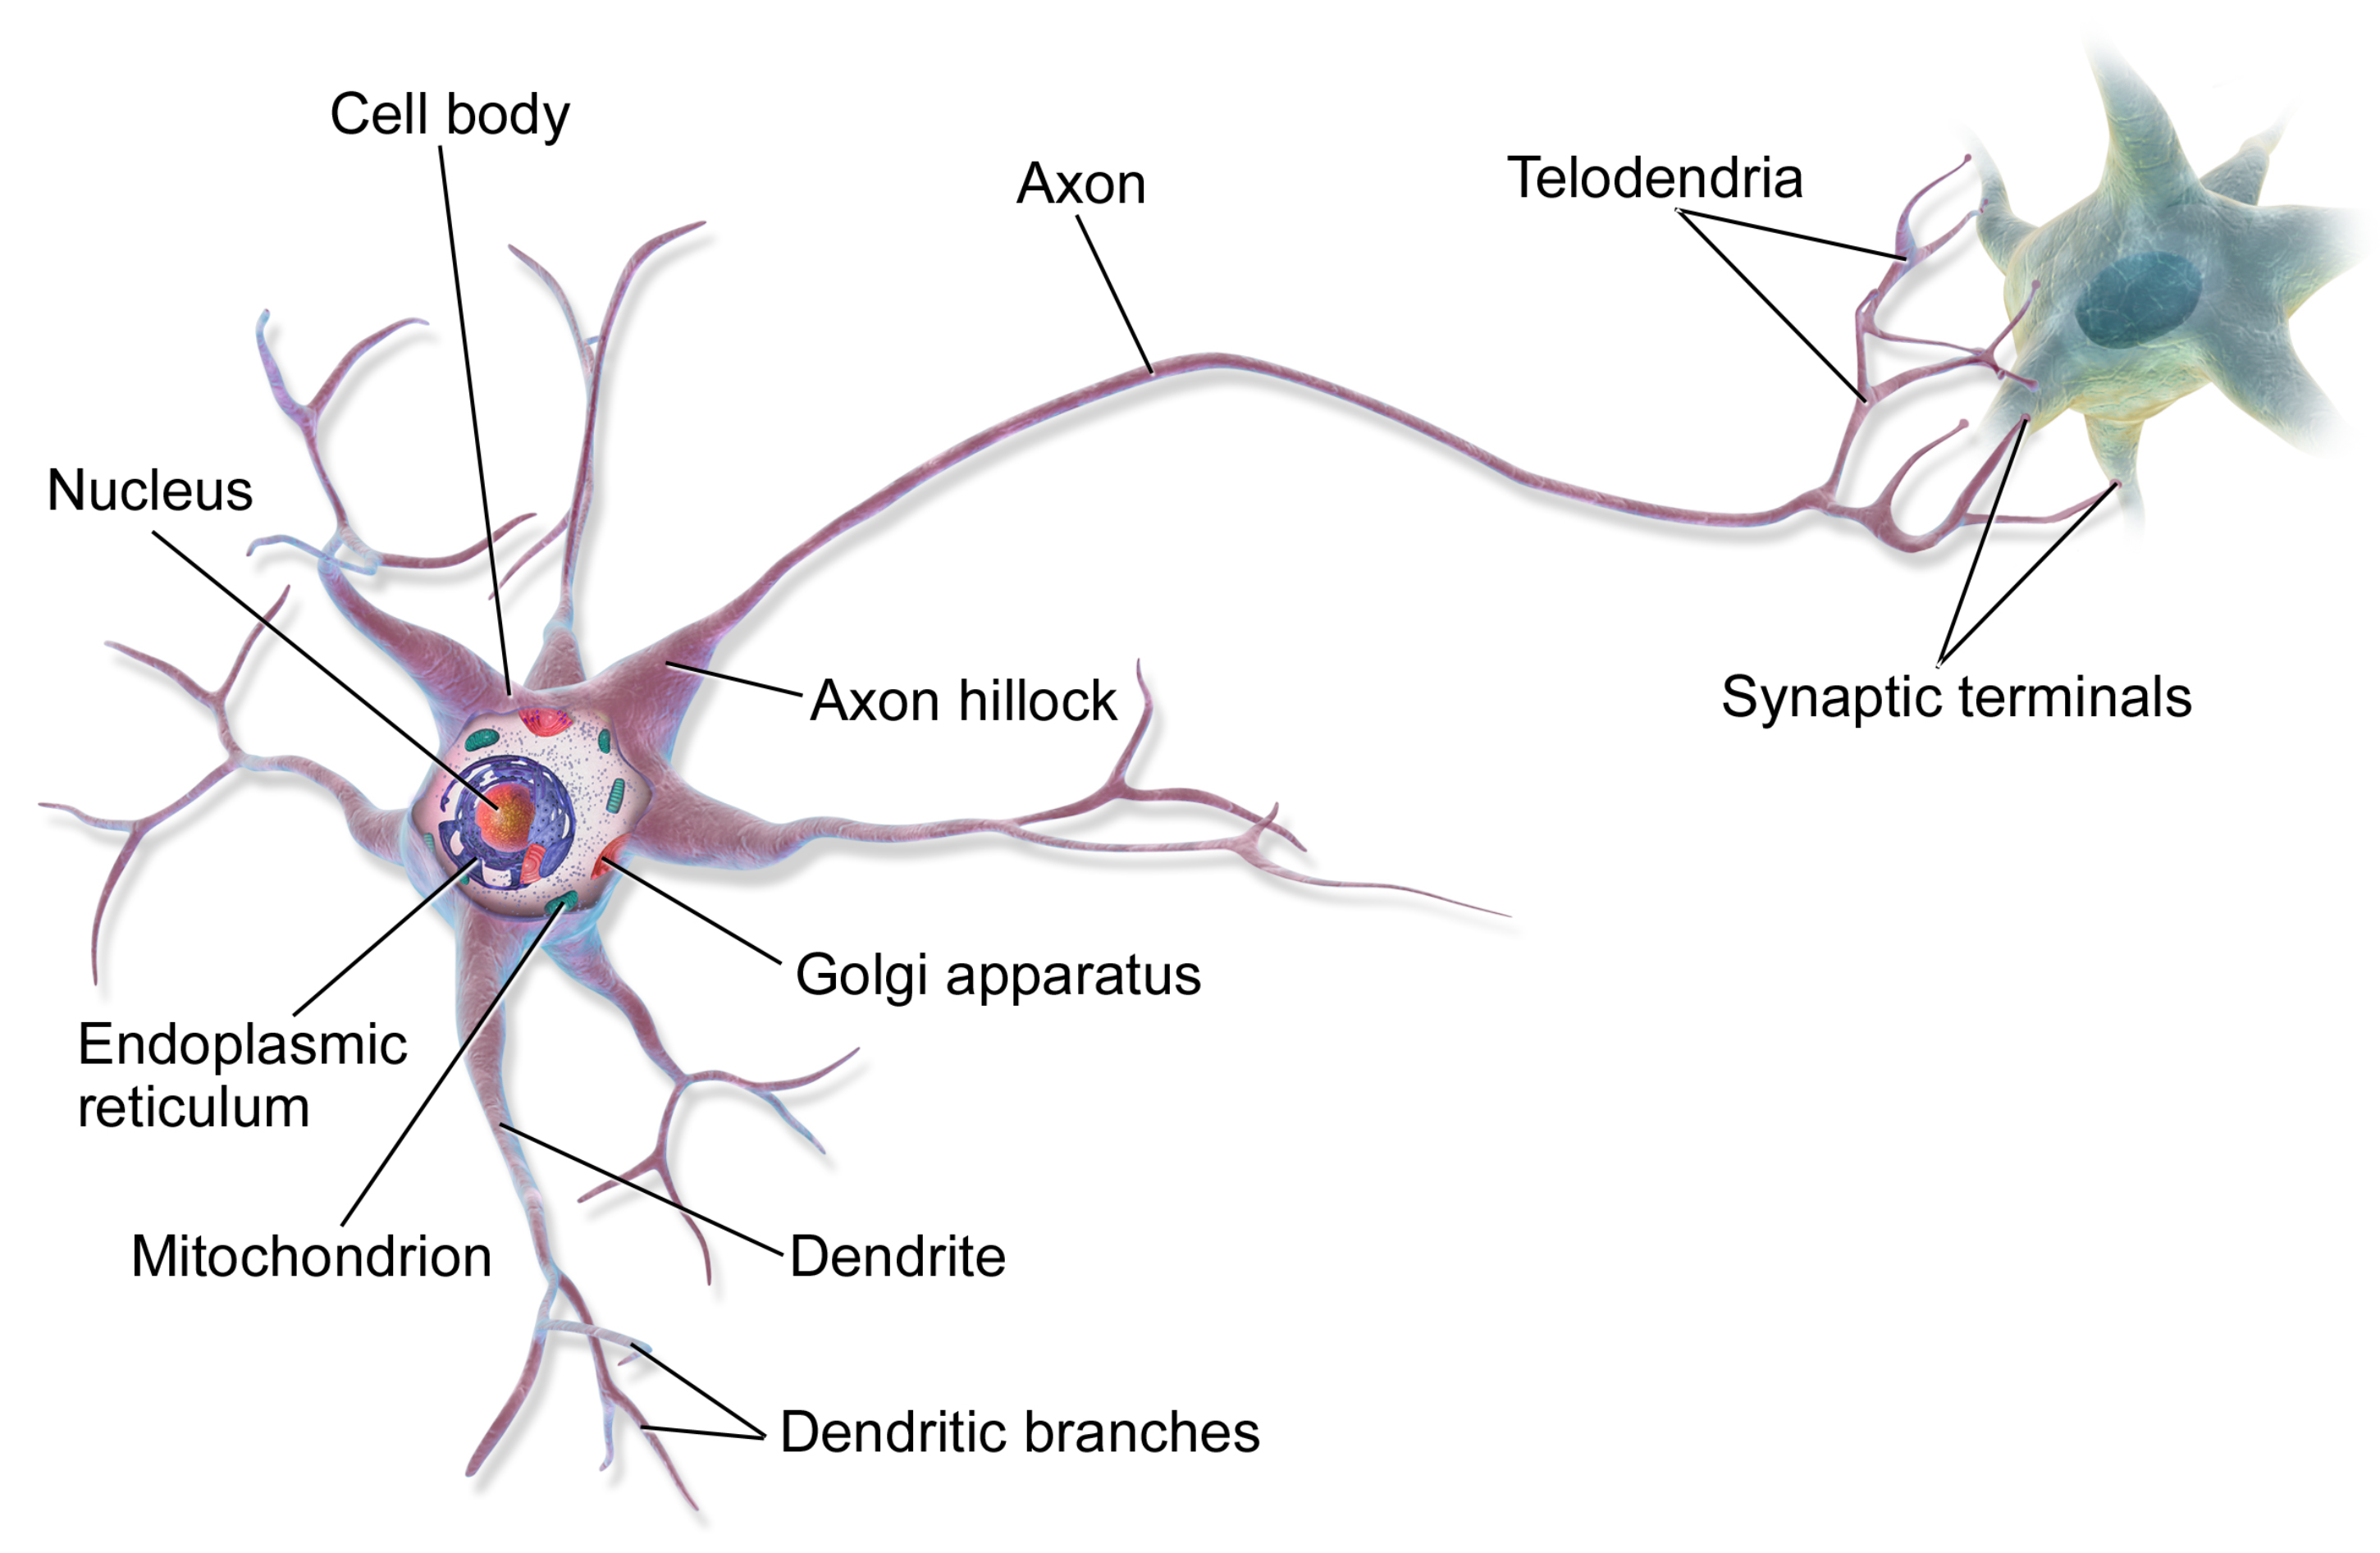
\includegraphics[width = 0.75\textwidth]{images/introduction/neuron_anatomy}
	 \def\c{Cartoon showing the basic anatomy of a neuron cell. }
	
	\caption[\c]{\label{fig:neuronanatomy} \c Of particular interest is the cell body (soma) and the protruding neurite (axon) which terminates on an adjacent cell body via a synaptic link provided by the dendrites. Figure adapted under a free to use license from the Wikipedia foundation \cite{neuronimage}.} 
\end{figure}
The morphology of neurons is a well-established and still active field of research \cite{Chen2012-qw} . There are a diversity of neuronal and dendritic structures each specialised to performing a particular task \cite{Squire2012-ru}.

This work will focus on the set of connections made in the superior colliculus by specialised neurones in the retina called retinal ganglion cells (RGCs). The superior colliculus in mice is a region of the midbrain which processes various sensory modalities, notably visual, auditory, and somatosensory information \cite{Seabrook2017-fa}.  In the superior colliculus there has not been an extensive classification of cell morphologies, although RGCs morphologies are well understood \cite{Ito2018-ef, Baden2016-kx, Gale2014-ss}. It is sufficient to consider that an RGC axon branches out into a relatively constrained and connected disk in its post-synaptic target area which can be seen in Golgi stains and microscopy studies of the mouse and related organisms \cite{Valverde1973-ws, Paxinos2014-kq}. It therefore has an ordered projective field and a continuous subset of the post-synaptic area has an ordered receptive field; see Section \ref{section:receptivefield}.

\subsection{Receptors and Ligands} \label{section:ephephrins}
Receptors are proteins, and ligands are molecules that have chemo-affinity with such proteins which is typically conferred by compatible binding domains \cite{noauthor_undated-od}. The Eph receptor is a tyrosine kinase protein that has an associated ligand called an ephrin both of which are membrane bound ensuring that cells physically contact during binding \cite{Beckmann1994-gx, Hirai1987-cx}. This class of molecules is ubiquitously expressed in many biological systems including the system of interest and are often involved in cell motility and guidance\cite{noauthor_undated-od}. Both Ephs and ephrins are able to signal, or interact, with other Ephs and ephrins and these interactions typically cause a cell to either experience an attractive or repulsive force based on relative levels of the available molecules. Most frequently two cells will express both Eph and ephrins and will therefore signal bidirectionally; see \cite{eph-ephrin-web}.
\begin{figure}[hb!]
	\centering
	\includegraphics[width = 0.75\textwidth]{images/introduction/eph-ephrin-binding}
	\def\c{Cartoon of a basic Eph-ephrin binding relationship. }
	
	\caption[\c]{\label{fig:ephrinbinding} \c Mutually compatible molecules come in physical contact on the cell membrane causing a reaction with some given affinity. Both the Eph and ephrin expressing cells receive a signal as a result of the reaction and the Eph expressing cell is said to receive the forward signal while the ephrin expressing cell is said to receive the reverse signal. Contact with the Eph-receptor by the ephrin ligand induces the forward signal in the Eph-receptor expressing cell. There are two major classes of Ephs and ephrins collectively referred to as A and B systems; within these systems there are many homologous molecules which have similar functions and can usually interact similarly with other molecules in the member class. The reaction can induce cell motility and this can be an attractive or repulsive movement and the repulsive actions are typically found in the A system while the attractive actions are found in the B system. Figure adapted under a free to use license from the Wikipedia foundation. \cite{ephrinimage}} 
\end{figure}
\subsection{Topographic Maps}
The final part of the fundamental biology to comment on is the notion of topographic maps. These are ubiquitous brain structures shared across multiple species and brain regions defined by an intuitive principle: physically neighbouring cells in some pre-synaptic region map to physically neighbouring cells in some post-synaptic region \cite{Swindale1996-kk, Cang2013-dw}. These maps a subset of the more general cortical map which share topological or continuous relations with multiple variables other than position e.g. direction and orientation selectivity for different stimuli \cite{Bednar2016-lg}. Most typically the topographic relationship is thought of as a one-to-one bijection which is a naturally intuitive notion, see Figure \ref{fig:topographicmap},  but there are some some salient and often ignored considerations.

\begin{figure}[h!]
	\centering
	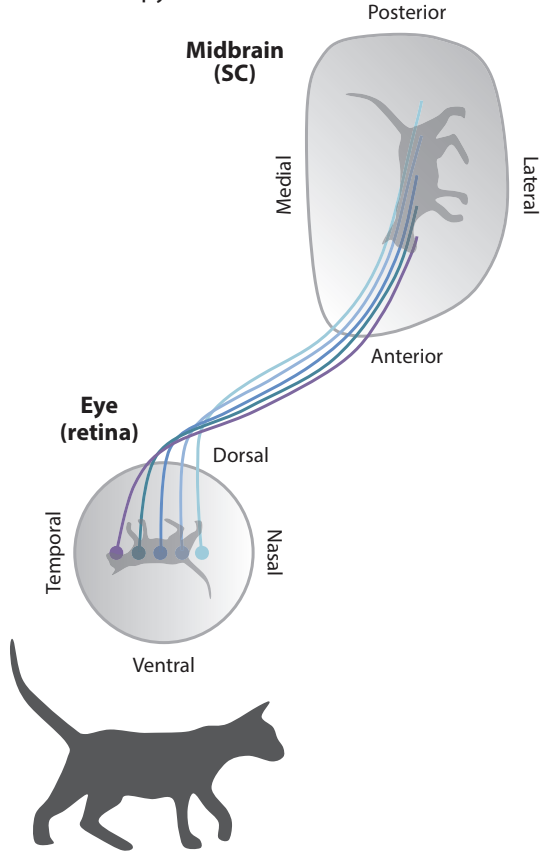
\includegraphics[width = 0.75\textwidth]{images/introduction/cartoon_topography}
	\def\c{Cartoon showing the retinotopic projection and relationship with the visual field. }
	\caption[\c]{\label{fig:topographicmap} \c Here a cat is presented as an image to a mouse's retina. This image is inverted by the lens of the eye and projected topographically into the SC where the neighbour relationships can be traced using the colour gradient. Figure adapted from Seabrook et. al. (2017) \cite{Seabrook2017-fa}.} 
\end{figure}
\subsubsection{Receptive and Projective Fields} \label{section:receptivefield}
The receptive field of a cell in the post-synaptic target is defined as the set of points in the stimulus field which the cell responds to \cite{Sherrington1906-et}; these are indicated by blue cones in Figure \ref{fig:projectivereceptivefield}. The projective field of a cell in the pre-synaptic target is the set of all points in the post-synaptic target that have synaptic contacts with that cell \cite{Lehky1988-nt}; these are indicated by the red cones in Figure \ref{fig:projectivereceptivefield}. These point based definitions can be natural extended to volumetric definitions by defining the projective/receptive field as the union of all point-wise fields in the area. 

\begin{figure}[h!]
	\centering
	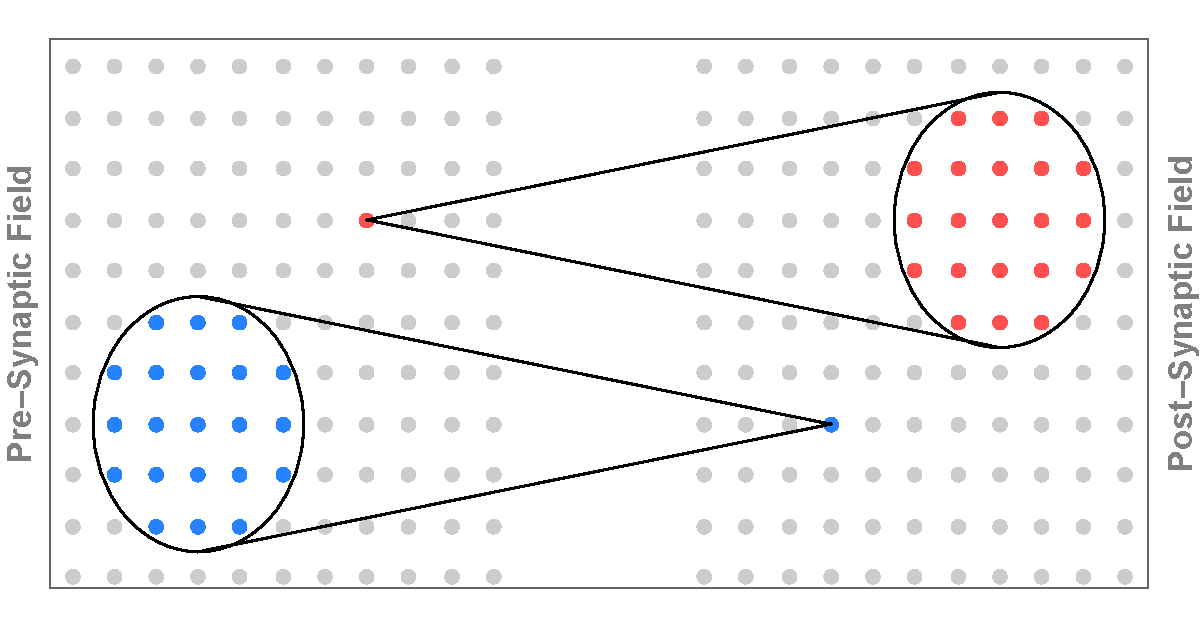
\includegraphics[width = \textwidth]{images/introduction/receptiveprojectivefields}
	\def\c{The pre-synaptic and post-synaptic fields are represented as ordered grids on the left and right respectively. }
	\caption[\c]{\label{fig:projectivereceptivefield} \c The receptive field is highlighted in blue with the blue node in the post-synaptic field responding to all blue nodes in the pre-synaptic field. The projective field is highlighted in red with all red nodes in the post-synaptic responding to the activation of the red node in the pre-synaptic field.} 
\end{figure}
If $f$ defines the projective field of a pre-synaptic point $i$ the mathematical definition is counter-intuitively the surjective map $f^\prime$ from the post-synaptic field to this point because function mappings cannot be many to one. This clarifies a problem with the discussion of projective and surjective fields: they are strictly not inverses of each other as the only way this is possible in a discrete context is for the map to be bijective. Each data source which attempts to detail these fields must be carefully analysed before conclusions are drawn.
\subsubsection{Dimensional Space of Developmental Topographic Mapping \label{sec:dimensionspace}}
The notion of projective and receptive fields can be unintuitive. It is generally easier to consider the topographic map as a function $W: \mathbb{R}^4 \rightarrow \mathbb{R}$ where $(x, y, \eta, \zeta) \mapsto w$, where $x$ and $y$ are coordinates in the pre-synaptic field, $\eta$ and $\zeta$ are coordinates in the post-synaptic field, and $w$ is the weight of the association between them. When considering development over a given timescale this definition can be extended to $(x, y, \eta, \zeta, t) \mapsto w$.
\section{Mouse Physiology, Anatomy, and Developmental Pathways}
The mouse retina has the geometry of a hemisphere (it is natural to represent it by a circular cross-section when it is flattened) and measures approximately 3mm in radius while the superior colliculus and adopts the approximate geometry of an ellipse with a greater diameter of approximately 2mm and a lesser diameter of approximately 1mm \cite{Park2012-yn, Seabrook2017-fa}. The superior colliculus of the mouse is located in the mid-brain and is organised in several different synaptic layers \cite{Ito2018-ef}. The superior colliculus acts to integrate and process multiple streams of sensory information as well as transmitting signals involved in movement: head shifting, escaping behaviour and freezing behaviours \cite{Ito2018-ef}. The inputs to the SC are varied with both external origin (e.g. retina) and inter-cortical origin (e.g. V1). This thesis is concerned with the organisation of the bundle of afferent neurons originating from the retina, specifically the RGCs, and terminating in the superficial layer of the SC; referred to as SC unless otherwise specified.
	
There are currently thought to be up to 42 different RGC types in the mouse retina with each of these thought to respond to specific elements of the visual field \cite{Goetz2022-ew, Baden2016-kx}. Each of the functions of these cell types will not be detailed but for further discussion about cell type classification, discussion, and potential issues see Sanes et. al. (2015) \cite{Sanes2015-xq}. A degeneracy amongst these cell types is now assumed and the pertinent mechanisms that guide them in forming a topographic map are considered rather than their ultimate cell fate. This simplifying assumption is legitimised by the fact ligand gradients are formed in the retina prior to RGC differentiation as will be made clear in the following discussion \cite{Marcus1996-kh}.

Cells in the retina and the SC express dual gradient and counter-gradients of Ephs and ephrins aligned along two characteristic orthogonal axes \cite{Marcus1996-kh, McLaughlin2005-jd, Lemke2005-iz}. The A system is arranged along the nasal-temporal (NT) axis in the retina and along the anterior-posterior (AP) or rostral-caudal (RC) axes in the SC. Here, EphA increases nasal-temporally and caudal-rostrally while ephrinA increases temporal-nasally and rostral-caudally. The B system is analogously arranged along the dorsal-ventral (DV) axis in the retina and the lateral-medial (LM) axis in the SC. Here, EphB increases dorsal-ventrally and medial-laterally while ephrinB increases ventral-dorsally and lateral-medially; see Figure \ref{fig:gradients}.

\begin{figure}[h!]
	\centering
	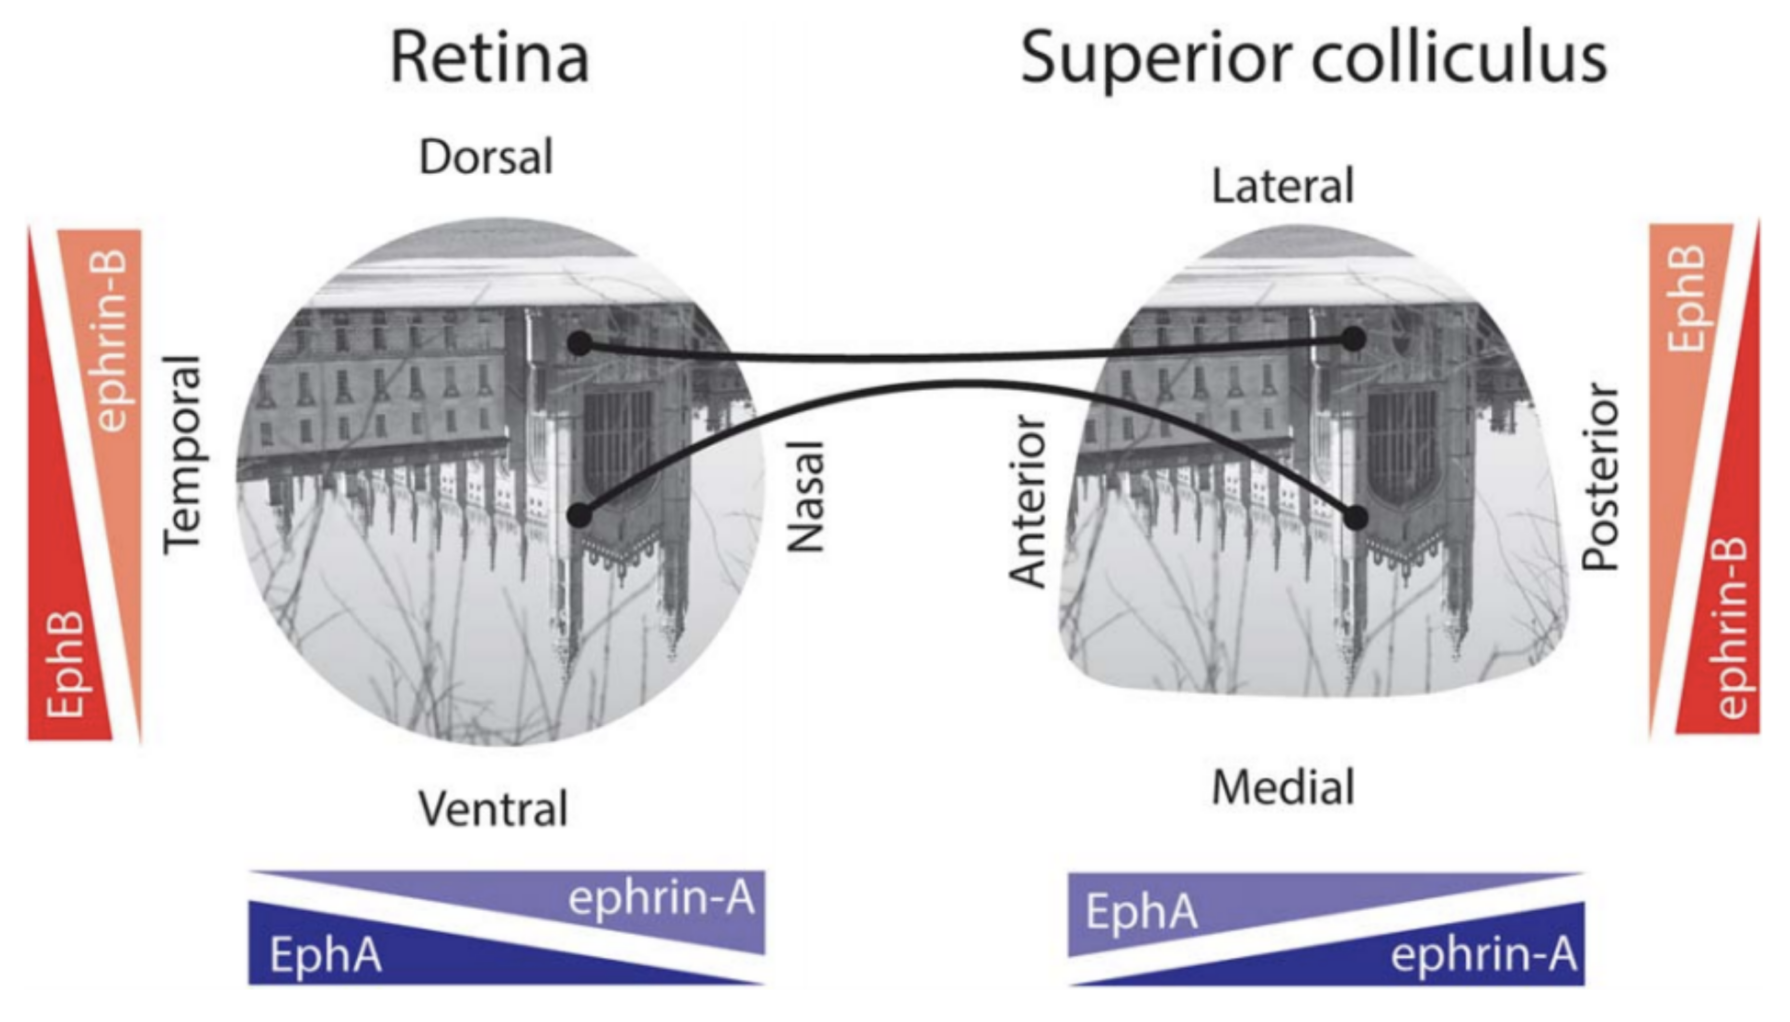
\includegraphics[width = 0.8\textwidth]{images/introduction/hjorth_gradients}
	\def\c{Each of the retina and SC have gradients and counter-gradients of EphA/B receptors and ephrin-A/B ligands with the A and B systems acting perpendicular to each other. }
	\caption[\c]{\c The chemotaxis then drives retinal locations to assigned SC locations preserving neighbour-neighbour relations through the graded expressions and establishing topography. Figure adapted from Hjorth et al. (2015) \cite{Hjorth2015-le}. \label{fig:gradients}} 
\end{figure}


The afferent neurons originating in the retina migrate towards the SC in a bundle passing through the optic chiasm where some pre-sorting is thought to occur \cite{Plas2005-yb}. Approximately 95\% of the afferents pass over the chiasm forming the contralateral projection into the SC and the remaining 5\% form the ispilateral projection \cite{Drager1980-px, Herrera2003-td, Koch2011-qz, Petros2008-rd}. The axon bundle makes a characteristic 90$^\circ$ turn before arrival at the SC. Each afferent then makes a characteristic overshoot of its eventual termination zone \cite{Yates2001-ug}. The overshoot is accompanied by interstitial branching into dendrites which, over time, are refined to a precise termination zone where the axon makes it final dendritic contacts \cite{McLaughlin2005-jd}. The termination zones typically occupy approximately $1$\% of the SC area \cite{McLaughlin2003-yy}. Each termination zone is defined by a characteristic location corresponding, in the wild-type, to a specific location of the visual field.

\section{Measurement and Data Analysis}

The modelling of the development of topography is driven by theoretical considerations but these are only relevant in the context of ground truth scientific data. These data will naturally be bound and constrained by the methods used to generate them and this section will detail some key data generation paradigms: surgical intervention, fluorescent dye focal injections, electrophysiology and multi-electrode arrays, calcium imaging, and intrinsic optical imaging.

\subsection{Microscopy}
Microscopy here will refer to fluorescence microscopy and can be subdivided into three distinct regimes: epifluorescence, confocal, and 2-photon. These three regimes are thought of as advancements of the same principle to produce higher quality images. Epifluorescence is the essential technique and relies on the principle of exciting a fluorophore with a wavelength that will cause it to fluoresce and measuring the emitted light. Confocal microscopy relies on the same emission principles as epifluorescence microscopy but uses a set of scanning mirrors and a pin-hole to improve the signal-noise ratio \cite{Inoue2006-rk}. Two-photon microscopy does not rely on the pinhole effect to generate in-focus images but rather the principle of two-photon absorption: two photons with roughly half the energy required to excite a fluorophore come together in a single quantum event and allow an emission photon \cite{Denk1990-ub}.

\subsection{Tracer Injections}
A tracer injection experiment injects a small amount of tracer material, typically DiI, into either the retina or the SC and allows it to diffuse into the opposing region \cite{Honig1989-by}. An injection diffusing from the SC to the retina is called retrograde, and from the retina to SC is anterograde. DiI is a compound which fluoresces and has the property that it diffuses laterally through the cell but not into other cells \cite{Sherazee2013-ky}. 

After a few days the retina and SC are removed and flattened and the amount of DiI is calculated through a microscopy measurement; see Figure \ref{fig:dii}. The resulting images then give a measure of the area of projection size to injection size and thus the ratio between two regions in the retrograde or anterograde projection can be calculated. Due to the diffusive nature of the procedure it is restricted to a limited region of either projection --- if multiple injection sites are used then the entire SC or retina will fill with DiI and no meaningful information can be gathered. This problem can be slightly mitigated by using DiI tags which fluoresce at different wave-lengths (green and red are typical) but this still limits the procedure to two injection sites; attempts to use more dyes have been thus far unsuccessful.

\begin{figure}[h!]
	\centering
	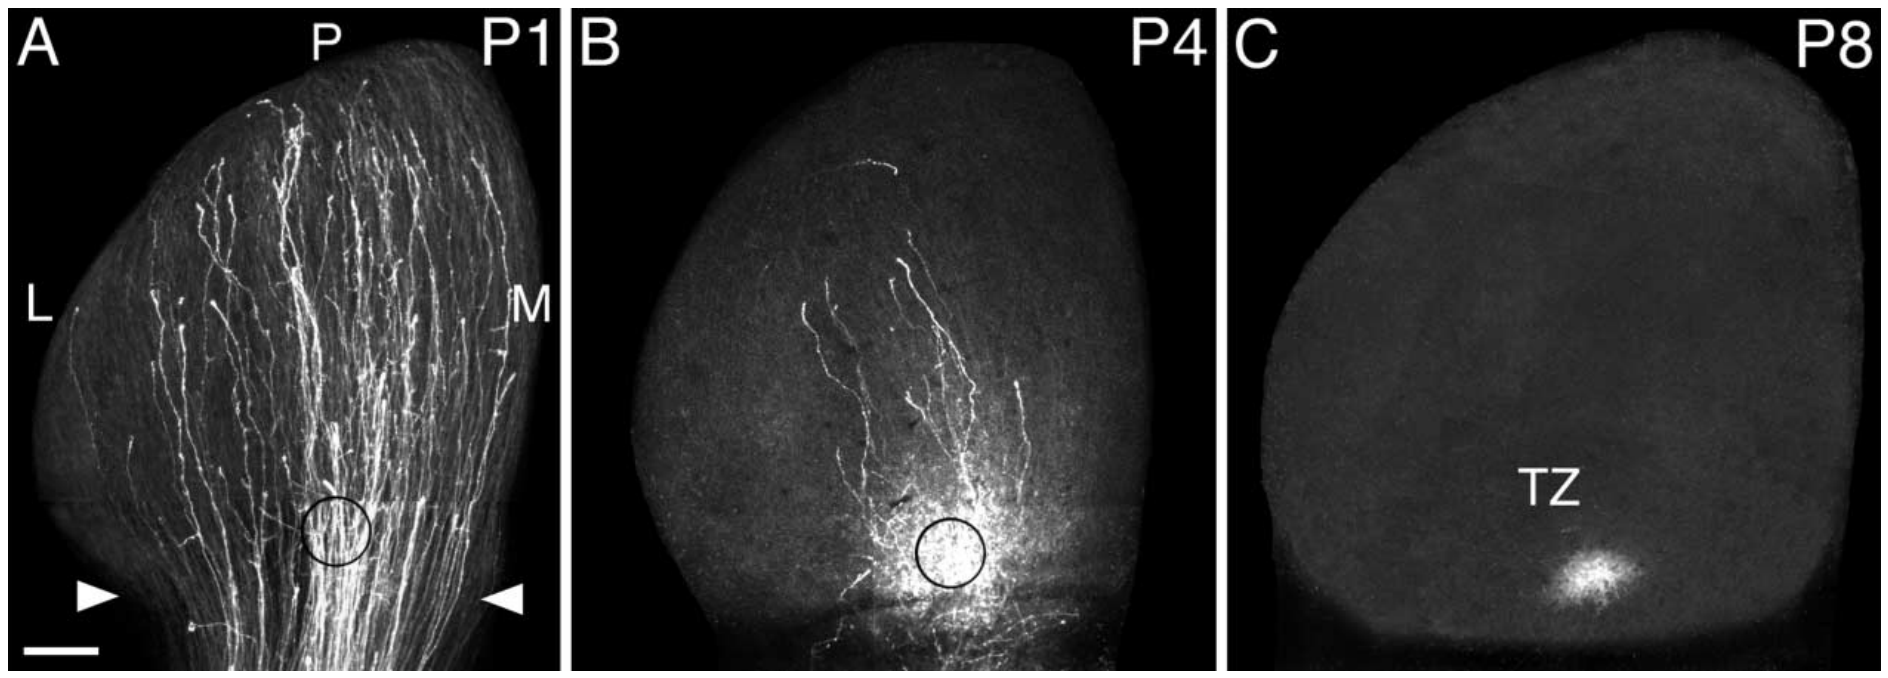
\includegraphics[width = \textwidth]{images/introduction/dii}
	\def\c{A typical experiment involving a series of DiI injections into the temporal retina at different developmental time points. }
	\caption[\c]{\label{fig:dii} \c The scale bar on the bottom left is $250\mu$m and the image covers the entire SC. The clarity of the image and the quality of the association with true anatomical features highlight the power of the DiI injection. The drawback is also highlighted because each injection at each time point represent a single pup that was killed to make the injection. Thus, no whole map can imaged from a single animal drastically reducing the conclusions that can be drawn about whole-map development. This problem is particularly pertinent in mutant studies where the map is drastically altered. Figure adapted from McLaughlin et. al. (2003) \cite{McLaughlin2003-yy}.} 
\end{figure}
\subsection{Calcium Imaging}
Calcium is used ubiquitously in biological systems as an intra-cellular and inter-cellular signalling mechanism. Notably, an influx of calcium in pre-synaptic terminals will trigger release of neurotransmitters and post-synaptically calcium transients appear to be key in mediating activity-dependent plasticity \cite{Grienberger2012-nr}. Therefore, calcium transients are a key indicator of cellular activity and can serve as a proxy for neuronal signalling. Calcium binds to several fluorescent proteins and these can be expressed in the specimen of interest  \cite{Grienberger2012-nr}. A microscopy technique can be used to stimulate the specimen over a time period and the changes in light intensity at a given location can be measured; see Figure \ref{fig:calcium}. The changes reflect the concentrations of calcium as the calcium binds to the available fluorophore and therefore the transient calcium levels in the specimen at the location of a given cell can be measured and used as a proxy for neural activity. 

\begin{figure}[h!]
	\begin{subfigure}{0.3\linewidth}
		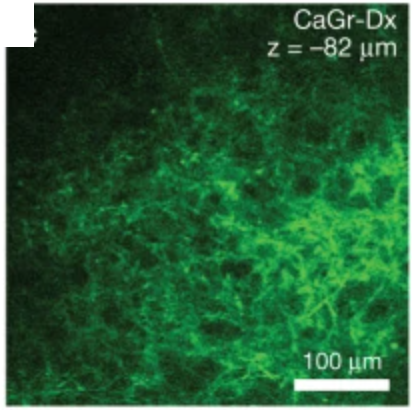
\includegraphics[width = \textwidth]{images/introduction/calcium1}
		\caption{} 
	\end{subfigure}
~
	\begin{subfigure}{0.4\linewidth}
		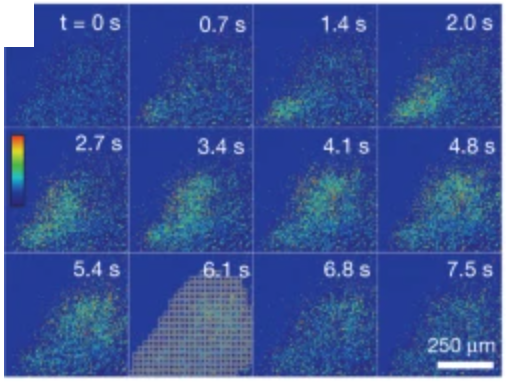
\includegraphics[width = \textwidth]{images/introduction/calcium2}
		\caption{} 
	\end{subfigure}
~
	\begin{subfigure}{0.2\linewidth}
		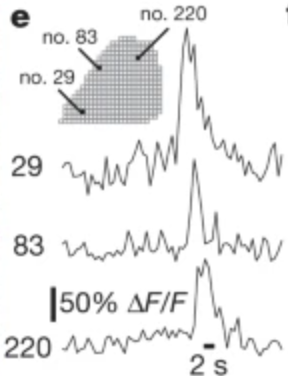
\includegraphics[width = \textwidth]{images/introduction/calcium3}
		\caption{} 
	\end{subfigure}
	\def\c{A series of images detailing the transient calcium imaging procedure. }
	\caption[\c]{\c First, confocal microscopy is used to image a small patch of the superior colliculus which has been tagged with a green fluorescent protein; (a). This imaging is performed over an extended time period and the intensity of the fluorescence is measured at every pixel of the image allowing for calcium transients to be recorded; (b). These transients can be examined at each location and give a proxy for neural activity and they may, for example, be associated with spiking events; (c). Figures reproduced from \cite{Ackman2012-uu}. \label{fig:calcium}}
\end{figure}


\subsection{Intrinsic Optical Imaging \label{sec:optical}}
The intrinsic optical imaging method uses a continuous periodic stimulation along which is then combined with concurrent passive activity recording to develop a map of mouse retinotopy \cite{Kalatsky2003-cz}. The advantage is that, while traditional methods rely on an input-output approach, this passive periodic recording allows systematic effects, errors, and noise to be averaged out.

The stimulation is provided to one eye by a small monitor presenting a single bar tracking in a horizontal or vertical fashion. The phase of the bar encodes the location in the visual field. The cortex is imaged using infra-red stimulation and recording through a charge-coupled device. The images are binned in time and the biological artefacts, such as the haemodynamic response, are removed by Fourier decomposition. This involves choosing a period of stimulation sufficiently different to known internal rhythms and selecting the harmonics with highest amplitude corresponding to the frequency of the drift grating. After this data is processed the response times of a location in the cortex is measured and due to the forward-reverse pattern of stimulation there will be two natural responses $s$ and $T-s$ for a period length $T$. These can be added and averaged to find the delay time of the system which should be uniform across the map, or subtracted and averaged to find the phase (visual field location) associated with that particular cortical region \cite{Kalatsky2003-cz}. In this fashion a whole map recording is made with some precision of a single specimen. These details are summarized in Figures \ref{fig:ois1} and \ref{fig:ois2}.
\begin{figure}[h!]
	\centering
	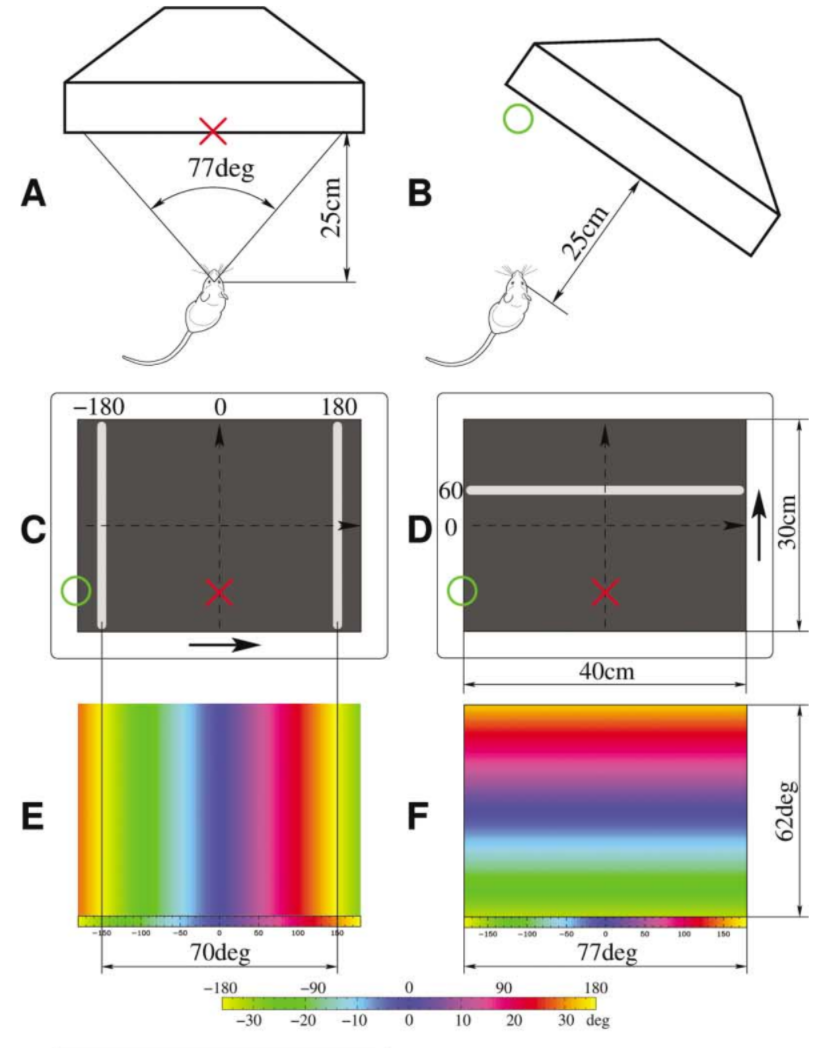
\includegraphics[width = 0.7\textwidth]{images/introduction/kalatsky_experiment}
	\def\c{The experimental procedure is detailed showing first the correct positioning of the stimulus screen for an ispilateral and contralateral stimulation (A) or a purely contralateral stimulation (B). }
	\caption[\c]{\label{fig:ois1}  \c The stimulus is presented as a series of horizontally (C) or vertically (D) drifting bars to measure azimuthal and elevational responses. The phase associated with each bar is mapped onto the colour schemes presented in (E) and (F). Figure adapted from Kalatsky and Stryker (2003) \cite{Kalatsky2003-cz}}
\end{figure}

\begin{figure}[h!]
	\centering
	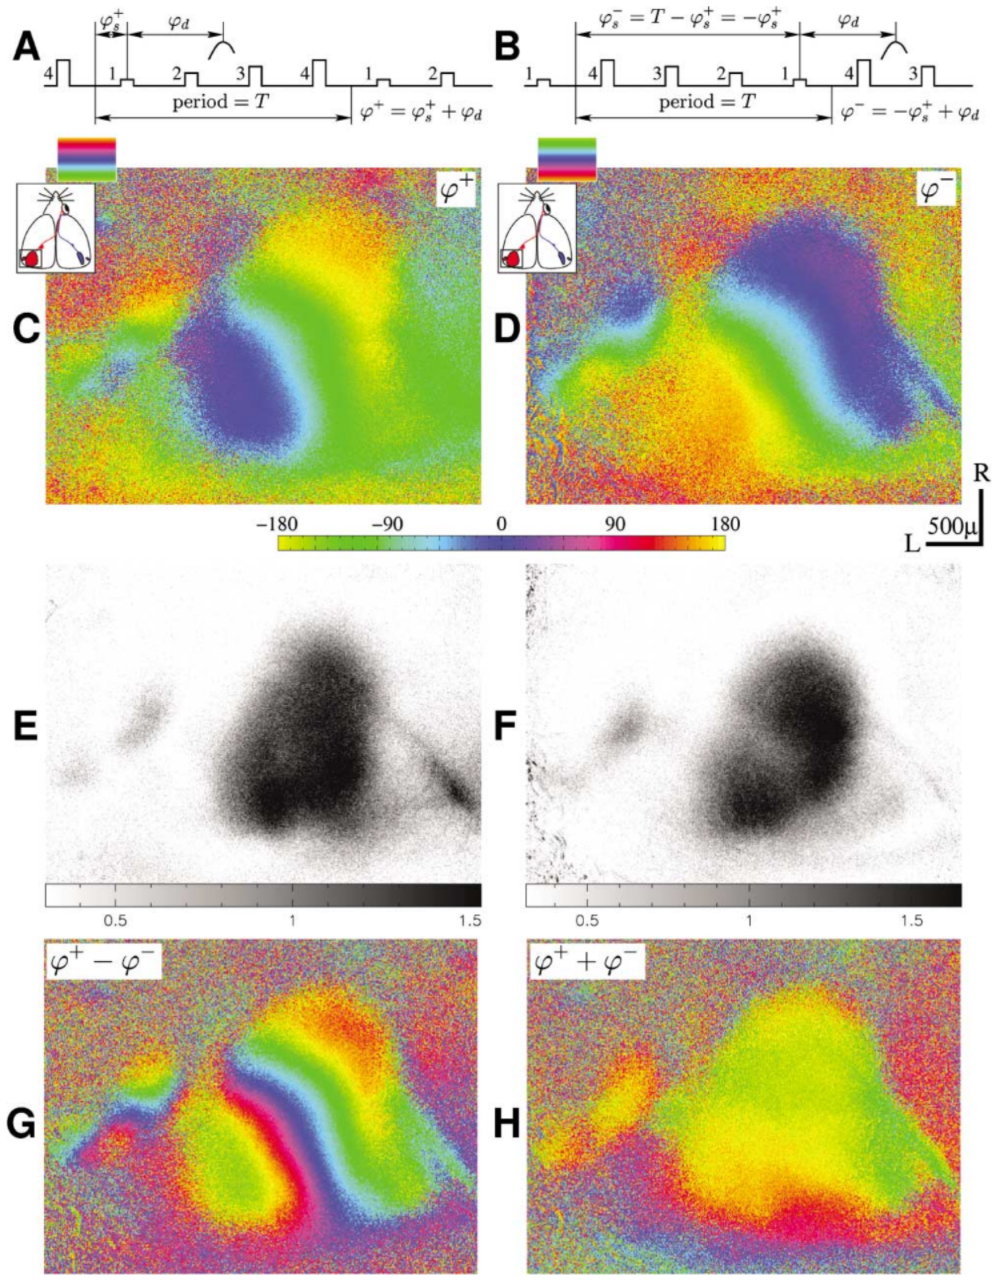
\includegraphics[width = 0.7\textwidth]{images/introduction/kalatsky_phase}
	\def\c{The experimental result is presented where forward drifting (A) and reverse drifting (B) bars are presented to measure the azimuthal response. }
	\caption[\c]{\label{fig:ois2}  \c The phase recordings for each of these stimuli are presented directly below in (C) and (D) and the bulk responses are presented in (E) and (F). The phase-delay trick is used to remove the haemodynamic response by subtracting the two phases giving the complete map in (G) and confirming a mostly uniform phase across the colliculus by adding the two phases and thus validating the method. Figure adapted from Kalatsky and Stryker (2003) \cite{Kalatsky2003-cz}.}
\end{figure}

\subsection{Electrophysiological recording}
Electrophysiological recording aims to make measurements of the electrical environment of a neuron at a given location, typically voltage, to understand the electrical activity of a cell. This can be translated into spike trains of action potentials which are of interest to understand the signalling relationship between two independently recorded locations.

The recording is made through an electrode which may record the activity at the membrane of a single neuron (single-unit) or multiple neurons (multi-unit). This may be done \textit{in vivo} or \textit{in vitro}. In a single electrode setup the receptive field of a neuron in the colliculus may be measured by stimulating various parts of the retina. This stimulation can be performed via visual stimulation (presentation of a visual image or scene), or via another electrode which stimulates a portion of the retina \cite{Boulton1990-ff}.

Multielectrode Arrays (MEAs) follow the same principle as single electrodes excepting that many channels/electrodes record simultaneously. This confers the advantage of regular sampling of a biological region with concurrent recording \cite{Potter2001-lg}. In this fashion broader statements about correlated regions over the colliculus can be made and more complicated phenomena with spatio-temporal characteristics, such as retinal waves, can be observed.
\subsection{Lattice Method \label{sec:lattice}}
While it is relatively straightforward to establish a feed-forward, or feed-backward association from any point in the pre-synaptic field or post-synaptic field it is relatively difficult to assess the quality of a map made from a collection of associations. Due to the complex nature of biological topographic maps whole-map analysis is often not performed. The Lattice Method is an algorithm designed to assess map quality in both forward and reverse directions \cite{Willshaw2014-ms}. The algorithm attempts to make a topographic matching between a pre-synaptic and post-synaptic field. First, the direction of the map is chosen by specifying which field is the image and which is the pre-image under the mapping: post-synaptic pre-image to pre-synaptic image or vice-versa. Second, a desired target spacing is specified and a selection of $N$ nodes from the all available points in the pre-image is made randomly in the following subroutine: chose a random unselected point and retain it if the spacing with already selected nodes exceeds the minimum spacing; if $N$ suitable nodes cannot be found after 10000 trials then restart the subroutine with the target of $N-1$ nodes. Once a selection of nodes has been made in the pre-image create a Deluaney tiling is made on the points defining these nodes \cite{Lee1980-wr}.  Each node in the pre-image is associated with a number of locations in the image given by the measured mapping. A bijection between the pre-image and image is created by associating each selected node in the pre-image with the average location of all points in the image it projects to. The edges of the Deluaney tiling are mapped under this bijection to create a graph in the image and any nodes attached to edges in the image-graph that intersect are removed to create a subgraph. The subgraph defines a well-ordered topographic mapping and the bijection restricted to this subgraph is a perfect topographic map. This procedure is summarised in Figure \ref{fig:lattice_procedure}. If the map is smoothly continuous then the amount of edges removed should be zero. Since the mapping is typically discrete there will be some removal of edges and the fraction of removed nodes gives an indication of the quality of the map.
\begin{figure}[h!]
	\centering
	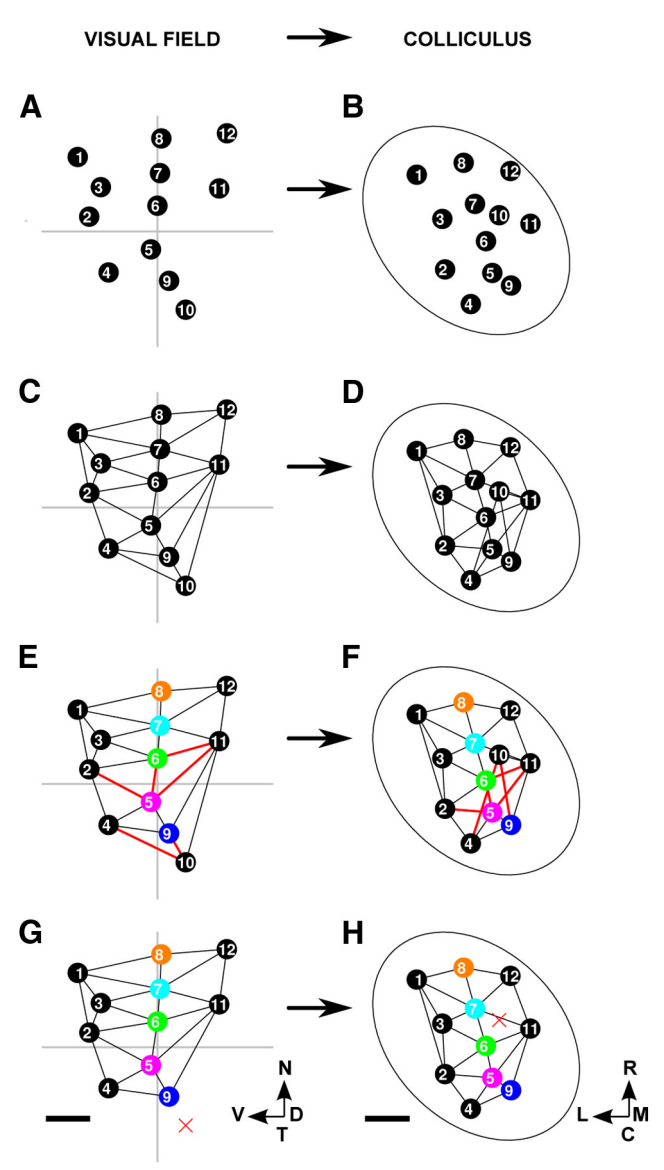
\includegraphics[width =0.6\textwidth]{images/introduction/lattice_procedure}
	\def\c{The method for creating a map with the visual field as the pre-image. }
	\caption[\c]{\label{fig:lattice_procedure} \c The points in (A) are first chosen according to the random sampling routine described in Section \ref{sec:lattice}. These are then mapped into the colliculus by finding their average synaptic location (B). A Deluaney tiling is made on the pre-image in the visual field (C) and the edges are placed on the nodes in the colliculus (D) under the same mapping as the points. Edges that are crossing in the image are identified and labelled in red (F) and mapped back into the pre-image (E). These edges are removed to give the largest submap with perfect topographic order (G-H). Varying the number and location of points in the pre-image can be used to determine map quality and reveal salient features of regular, but not wild-type, maps. Figure adapted from Willshaw et. al. (2014) \cite{Willshaw2014-ms}.} 
\end{figure}

It is important to note that $f: X \rightarrow Y$ and $g: Y \rightarrow X$ for arbitrary $g, f$ does not imply that $f^{-1} = g$. The Lattice Method therefore gives the quality of both the forward mapping as well as the reverse mapping between the pre-synaptic and post-synaptic fields. Figure \ref{fig:lattice_results} shows the Lattice Method applied to a wild-type mouse in forward and reverse directions.
\begin{figure}[h!]
	\centering
	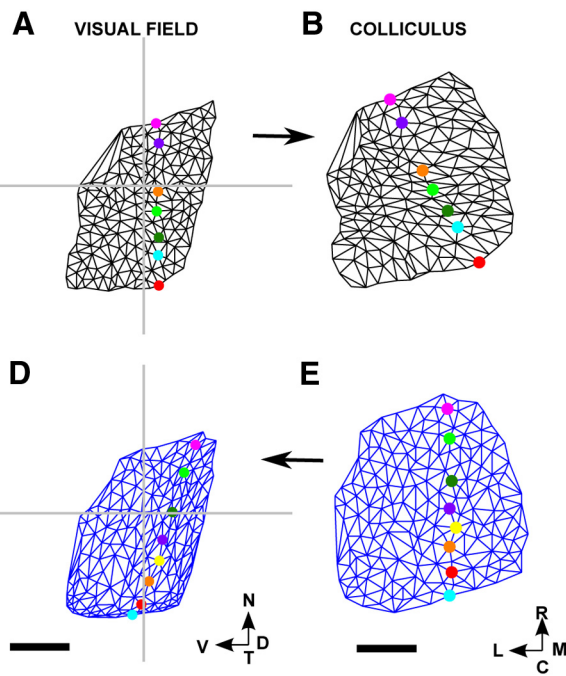
\includegraphics[width = 0.6\textwidth]{images/introduction/lattice_results}
	\def\c{The method can be applied with the visual field or colliculus as both the pre-image and the image respectively. }
	\caption[\c]{ \c Both maps constructed from optical image scanning of a wild-type mouse are shown in the right panel. The visual field as the pre-image is detailed in black,  and as the image in blue. A coloured code slice of the function is highlighted with a selection of nodes and the colouring reflects the topographic continuity. Figure adapted from Willshaw et. al. (2014) \cite{Willshaw2014-ms}. \label{fig:lattice_results}  }
\end{figure}

\FloatBarrier
\section{Mutant Mouse Observations}
The scientific understanding of the development of the retinotopic system, and indeed a large part of developmental biology, has been accelerated by genetic mutation studies; see section \ref{section:genemutations}. Several recent genetic manipulations that have been performed in mouse and their effects on the organisation of the topographic organisation will be detailed here and their theoretical implications of their observations discussed Section \ref{section:developmentaltheory}.
\subsection{Ephs and Ephrins}
In the case of the mouse retinotopic system there are two systems, labelled A and B, of Ephs and ephrins that are expressed in a gradient along orthogonal axes of the retina and the SC respectively, allowing for this bidirectional signalling to occur; see Figure \ref{fig:ephrinbinding}. The A and B systems are thought to have different interactions and are most often thought to act independently of one and other; for a summary of these interactions see Table \ref{table:ephephriniteraction}. A series of studies has confirmed the existence of several classes of both A and B molecules and these are thought to interact in similar ways; the interaction properties of these subclasses are assumed to be degenerate. The gradients for the A system along the retina have been measured by and shown to follow a complementary pattern where the Ephs decrease in tandem with the increase of the ephrins \cite{Reber2004-wq}. This gradient-counter-gradient pattern was shown to be repeated in the SC allowing for bidirectional signalling to occur along the two axes. Interestingly, the B system is also expressed at the optic chiasm where the incoming retinal axon bundle diverges into the contralateral and ispilateral portions of the brain \cite{McLaughlin2003-co}.
\begin{table}
	\centering
	\begin{tabular}{|c|c c c c|}
		\hline
		\textbf{Molecular Type} & EphA & EphrinA & EphB & EphrinB \\
		\hline
		EphA & Attractive & Repulsive & None & Cross-talk* \\
		EphrinA & Repulsive & Attractive & None & None \\
		EphB & Cross-talk* & None & Repulsive & Attractive \\
		EphrinB & None & None & Attractive & Repulsive \\
		\hline
	\end{tabular}
	\def\c{A brief summary of the interaction properties of each of the major classes of Ephs and ephrins in the developing mouse retinotopic system. }
	\caption[\c]{\c Generally, the interactions between Ephs and ephrins is context dependent: they may be attractive, repulsive, or bifunctional; see Section \ref{section:ephephrins}. It should be noted that while much work has been done to establish the function of the EphA-ephrinA relationship there has been less work done on the EphB-ephrinB relationships or on the potential interaction between classes \cite{Lemke2005-iz}. EphA4 has been observed to bind with all ephrinBs and EphB2 can bind to ephrinA5 indicating a limited amount of cross talk between the two classes \cite{Gale1996-zd, Himanen2004-jj}. \label{table:ephephriniteraction}}
\end{table}
There are currently 14 identified classes of Eph receptors and 9 classes of associated ephrin ligands. These classes are subdivided into 8 classes of EphA receptors, 6 classes of EphB receptors, 6 classes of associated ephrin-A ligands, and 3 classes of associated ephrin-B ligands. The interaction of the tyrosine-kinase protein and its associated ligand is mediated by proximity: the ephrins are membrane bound and the Eph receptors will be stimulated by contact with this membrane. The receptor-ligand pairing occurs within all subclasses of an A/B grouping, but their does not appear to be interaction between A and B pairs with the exception of EphA4 which can bind to both ephrinAs and ephrinBs and EphB6 which can bind to ephrinA5 \cite{McLaughlin2005-jd, Lemke2005-iz, Gale1996-zd, Himanen2004-jj}.

The expression of these molecules is graded through both the retina and SC with the A and B classes being expressed perpendicular to each other. In mouse the retina expresses EphA5 and EphA6 in an increasing fashion from the nasal to temporal locations, EphA4 is expressed in an ungraded fashion (constant expression) across the retina, ephrin-A2 and ephrin-A5 are expressed in a decreasing fashion from nasal to temporal locations, EphB1-B4 and EphA6 are expressed in an increasing fashion from dorsal to ventral locations, ephrin-B1 and ephrin-B2 are expressed in a decreasing fashion, and ephrin-B3 is expressed in an ungraded fashion across the retina  \cite{McLaughlin2005-jd, Lemke2005-iz}. In the SC the EphA4, EphA3, and EphA7 are expressed in a decreasing fashion from the anterior to posterior locations, ephrinA2 is expressed in an increasing fashion anterior to posterior but then decreasing towards the final posterior locations, EphB1-B3 are expressed in a decreasing fashion from lateral to medial locations, and finally ephrin-B1 is expressed in an increasing fashion from lateral to medial locations. These gradients are summarised graphically in Figure \ref{fig:measuregradients}. The promiscuity of the various subclasses means that they are thought of as linearly additive resulting in a total gradient and counter-gradient in both orthogonal directions of both the retina and the SC. The graded expressions guarantee that for each position in the retina there is a unique position in the SC where chemotactic forces are balanced in all directions: the topography emerges from guidance to this position. This information is summarised previously in Figure \ref{fig:gradients}.

\begin{figure}
	\centering
	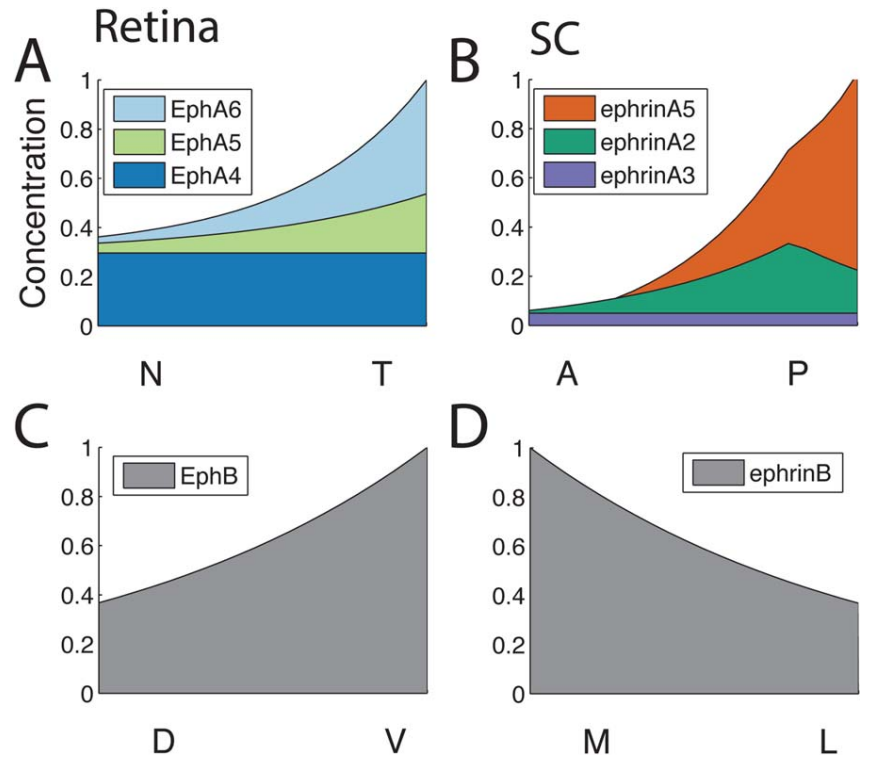
\includegraphics[width = 0.5\textwidth]{images/introduction/gradientsEphEphrinMeasured}
	\def\c{A cartoon of the primary gradient expression profile in the A and B systems in the superior colliculus and retina. }
	\caption[\c]{\label{fig:measuregradients} \c The A system has been measured by proxy of mRNA expression and the contribution of each subclass is coloured and displayed in (A) and (B). The EphA family generally has an exponential profile increasing from nasal to temporal regions of the retina with the exception of EphA4 which is expressed as a constant. The ephrinA family generally has an exponential profile increasing from anterior (rostral) to posterior (caudal) regions of the colliculus. The B system has few measurements available and is shown in grey in (C) and (D). The EphB  family is assumed to have an exponential profile increasing from the dorsal to ventral regions of the retina. The ephrinB family is assumed to have an exponential profile increasing from the lateral to medial regions of the colliculus. Figure adapted from Hjorth et. al. (2015) \cite{Hjorth2015-le}.}
\end{figure}
\begin{figure}
	\centering
	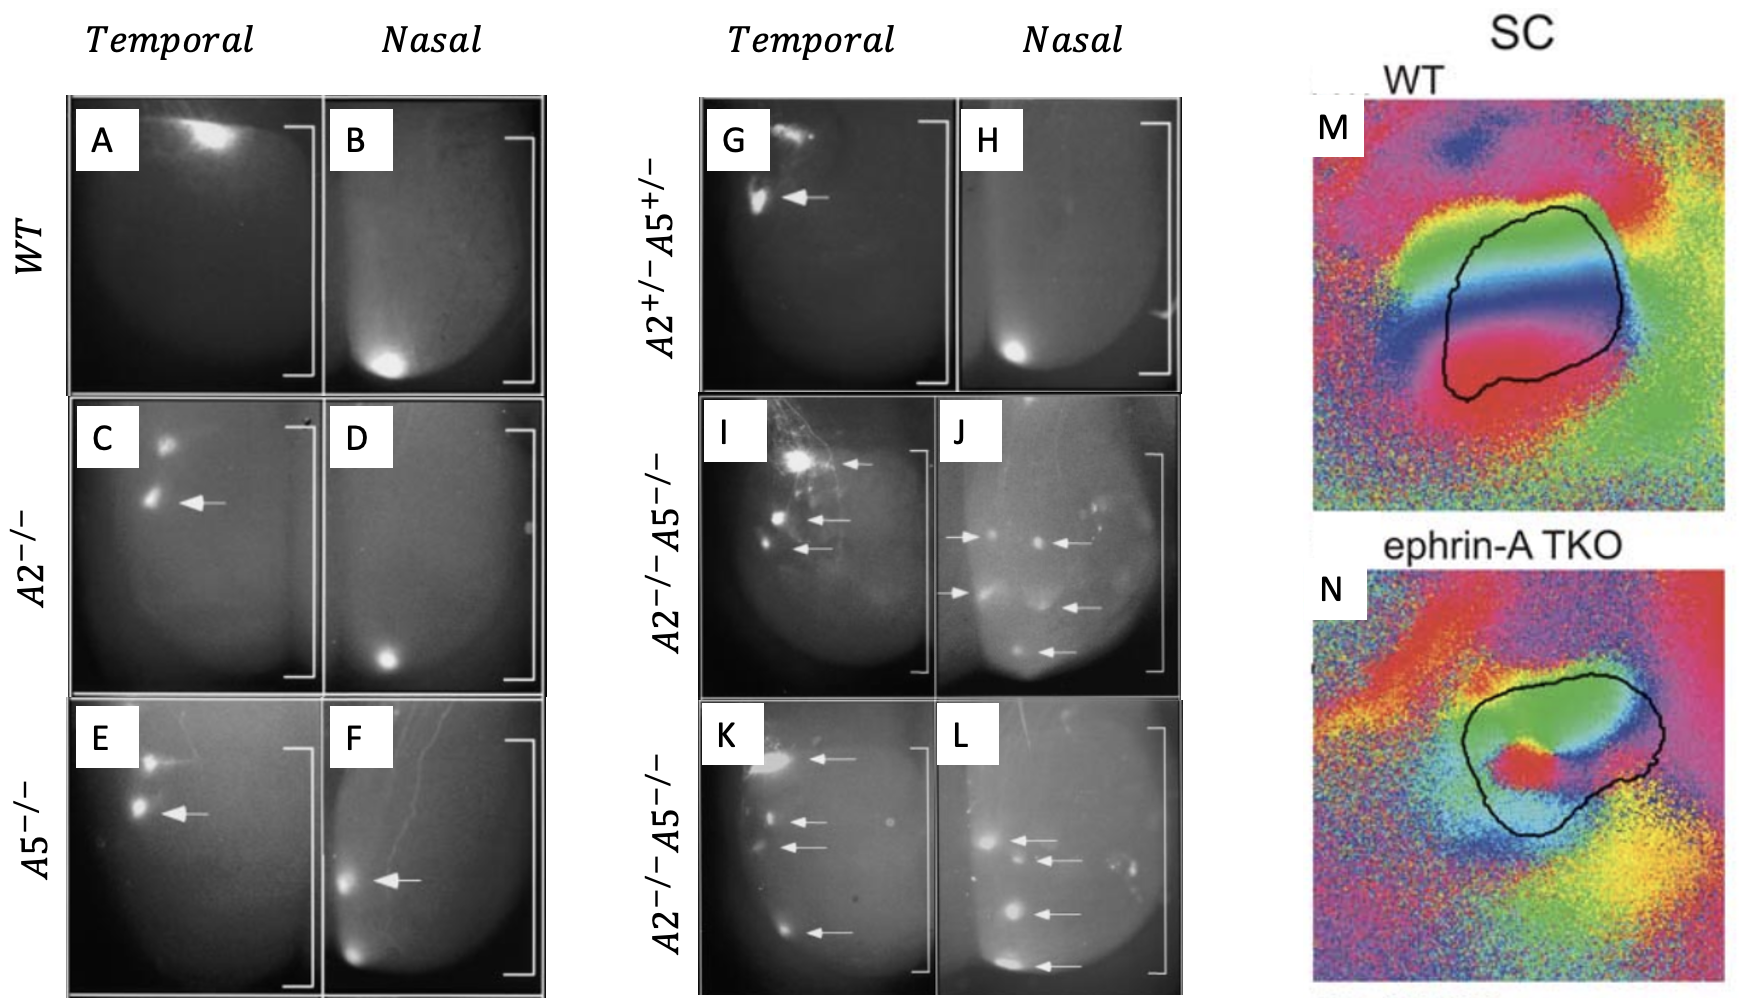
\includegraphics[width = 0.8\textwidth]{images/introduction/ephrinKO}
	\def\c{The effect of multiple combinations of single and double ephrinA2, ephrinA5, and ephrinA3 knock-outs. }
	\caption[\c]{\label{fig:ephrinknock-outs} \c A DiI injection is performed for wild-type (A and B), ephrinA2 double knock-outs (C and D), ephrinA5 double knock-outs (E and F), and ephrinA2A5 single knock-outs (G and H) while two examples of ephrinA2A5 double knock-outs are shown in (I-L). It can be seen that the double knock-out of ephrinA2 induces ectopic projections in the temporal retina while the double knock-outs of ephrinA5 induces ectopic projections across the whole NT. The single knockout of both ephrinA2 and ephrinA5 induces ectopic projections only temporally but these ectopic have less precisely defined projection zones. The double knock-out of ephrinA2A5 induced multiple ectopic projections across the entire NT-AP axis. The whole map in the ephrinA2A3A5 triple knock-out elevational and azimuthal scans are presented in M and N respectively. These reveal the disorder but notably demonstrates that there are still localised functional domains. Figures (A-L) adapted from \cite{Feldheim2000-ec}. Figures M and N adapted from \cite{Cang2008-ez}.}
\end{figure}
\subsection{EphrinA knock-outs}
One natural way to test the role of an Eph/ephrin is to knockout a component and observe the effect on topographic map formation; knockout experiments have been performed extensively in the context of the ephrinA system. These are the single knockout, double knockout, and triple knockout studies: ephrinA2 and ephrinA5 (single), ephrinA2A5 (double), and ephrinA2A3A5 \cite{Frisen1998-jw, Feldheim2000-ec, Cang2008-ez}. The effect of these is to largely disrupt the mapping along the NT-AP axis. EphrinA2 makes its primary contributions to the total ephrin gradient in the anterior colliculus, and accordingly in the ephrinA2 knock-down topographic order along this axis is primarily lost anteriorly. Similarly, the ephrinA5 contribution is most significant in the posterior colliculus and the ephrinA5 knock-down phenotype has a loss of order in this region. The ephrinA2A5 knockout combines these effects presenting a loss of order along the entire AP axis with multiple ectopic projections being observed for single retinal injection sites; see Figure \ref{fig:ephrinknock-outs}. The ephrinA2A3A5 knockout is similar, but the effect appears to be more pronounced with optical image scans showing a lack of order along the AP axis. Interestingly, some topographic order is preserved and the maps are not comparable to a random association between points on the AP and NT axes \cite{Willshaw2014-ms}. 


\FloatBarrier
\subsection{EphA3 knock-in \label{sec:epha3}}
The EphA3 knock-in involves inserting a non-endogenous Eph receptor in the Islet2 region of the mouse genome \cite{Brown2000-da, Reber2004-wq}. This insertion is particularly interesting because this region is only expressed in approximately 40\% of retinal cells and is not expressed in the SC \cite{Brown2000-da}. The expression pattern along the retina is often referred to as ``salt-and-pepper" suggesting that $Islet2^{+/-}$ cells are distributed randomly, but there is little work to formally establish the distribution \cite{Lemke2005-iz}. The addition of a constant amount of EphA3 to a fraction of RGCs induces an ectopic projection in the mapping into the SC but unlike the ephrinA knock-outs these ectopics have a stereotypical location which they project to; see Figure \ref{fig:epha3anatomical}. The heterozygous knock-in has ectopic projections from nasal regions in the retina but these collapse in temporal regions; see Figure \ref{fig:epha3collapse}B. The homozygous knock-in has a stereotypical ectopic projection for every point in the retina with no collapse point which creates a complete duplication of the topographic map both anatomically and functionally see Figures \ref{fig:epha3anatomical}, \ref{fig:epha3collapse}C, and \ref{fig:epha3functional}. This is most prominent in the double knock-in where there are therefore two complete representations of the visual field in the neural space occupied by the SC. It has been claimed that the $Islet2$ expressing and non-expressing cells are perfectly partitioned into the anterior colliculus (wild-type) and posterior colliculus (EphA3) \cite{Cang2013-dw}. 

\begin{figure}[h!]
	\centering
	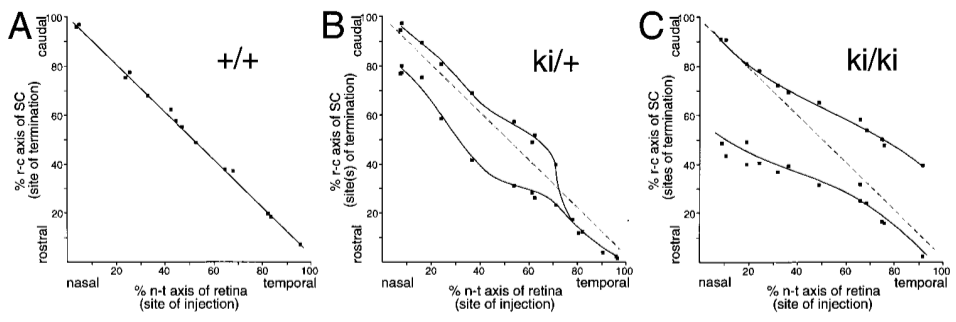
\includegraphics[width = 0.6\textwidth]{images/introduction/brownEphA3}
	\def\c{Bulk anatomical tracer experiments on the EphA3 knock-in mutant.}
	\caption[\c]{\label{fig:epha3collapse} The data points in each of the panels represent the location of the centres of tracer injection at a given retinal location.  The wild-type injections shown in panel A form a predictable straight line indicating an ordered topography. The heterozygotes shown in panel B have two projections in the nasal portion of the retina but these collapse to form a single projection as the injection site moves toward the temporal retina. The homozygotes shown in panel C also exhibit the stereotypical ectopic projection and there is no collapse point indicating the presence of two ordered topographic maps.  Figure adapted from \cite{Brown2000-da}.}
\end{figure}


\begin{figure}
	\centering
	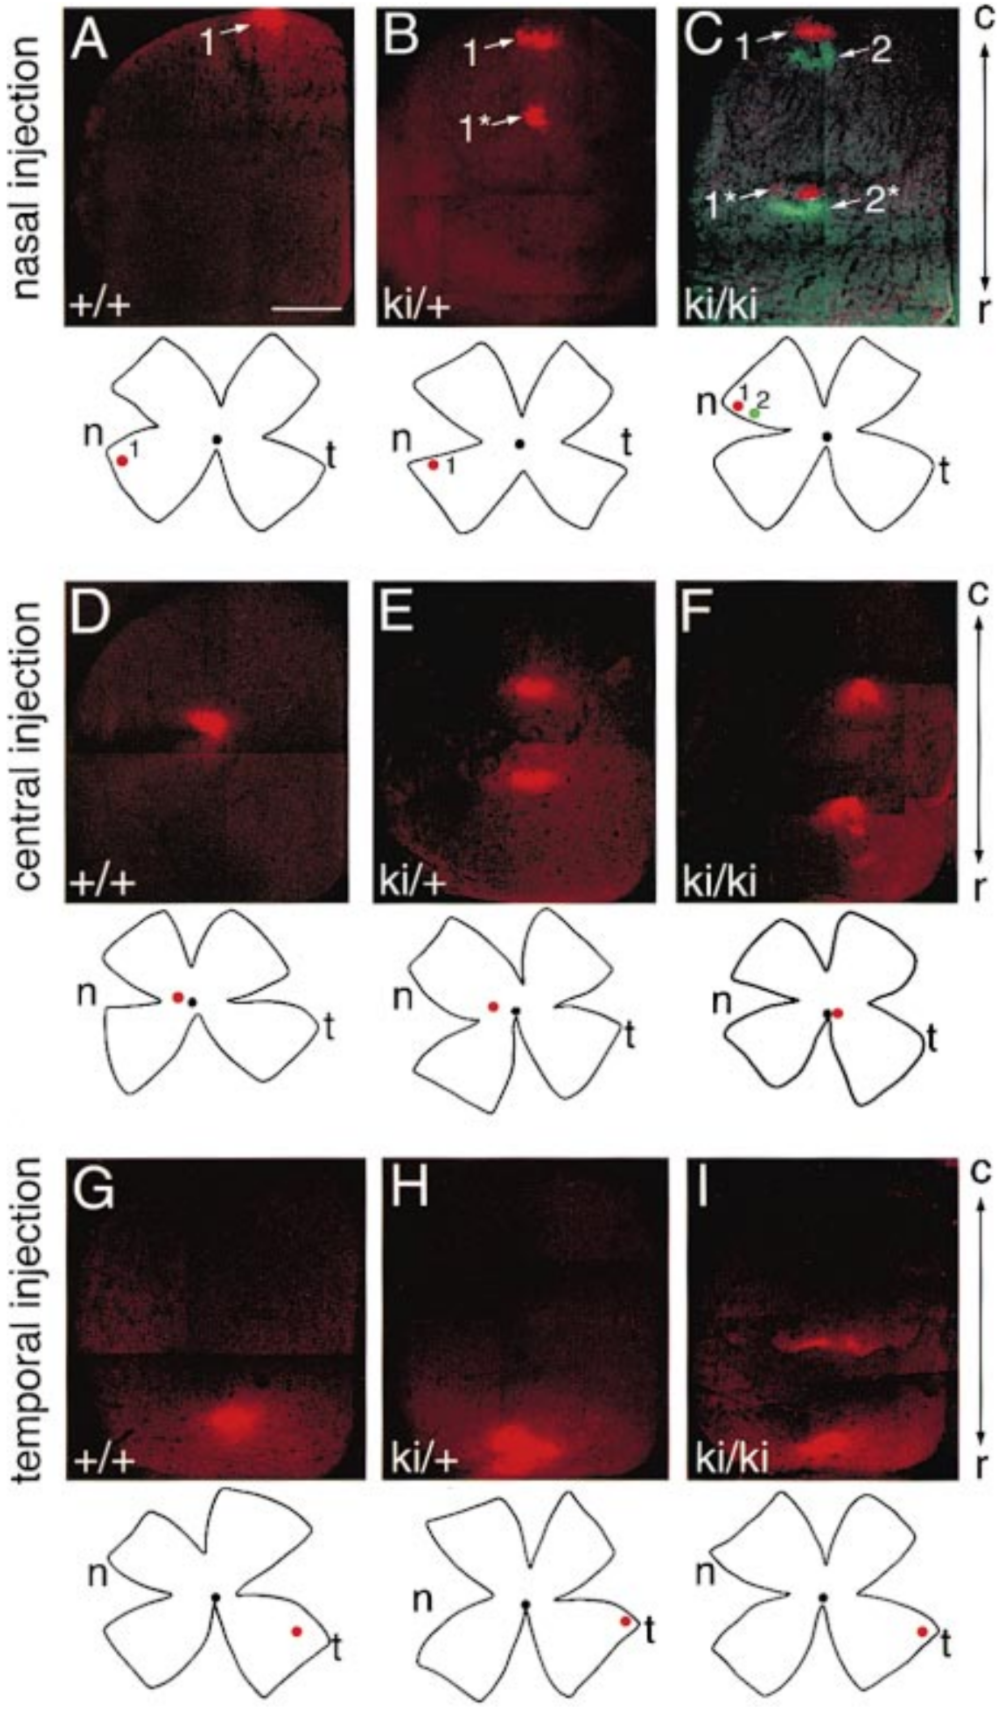
\includegraphics[width = 0.6\textwidth]{images/introduction/epha3anatomical}
	\def\c{Visualisations of the wild-type, heterozygous, and homozygous EphA3 knock-in mice. }
	\caption[\c]{\label{fig:epha3anatomical} \c An anterograde injection is made in the nasal, central, and temporal retina for a wild-type, heterozygous EphA3 knock-in, and homozygous EphA3 knock-in in the left panel (a). The heterozygote presents a duplicated projection in the caudal (posterior) and central regions but just one projection in the rostral (anterior) region. The collapse point of the map is where the two distinct mappings coalesce into a single mapping which can be seen in (B) at the 75\% tick of the NT axis. The homozygote has duplicated projections in all three regions. Two injections with different fluorescent tags are performed nasally in the homozygote demonstrating that the two projections maintain relative ordering. Figure adapted from \cite{Brown2000-da}.}
\end{figure}

The heterozygote is of particular interest. The anatomical collapse points in this mutant appear to have more variation than in the homozygote. Furthermore, the visual field maps produced by heterozygous specimens have widely varied visual characteristics which have been conjectured to arise from a stochastic interaction between chemotactic and activity-based development mechanisms \cite{Owens2015-zv}. Attempts have been made to categorise these variations but they have been inconclusive due to mathematical considerations of the methodology used, as well as labelling discrepancies in the data. Nevertheless, these specimens are a prime data-set to develop insights about the development effect of this mutant as well as generate and validate hypotheses from theoretical considerations. 

\begin{figure}
	\begin{subfigure}{0.625\textwidth}
		\centering
		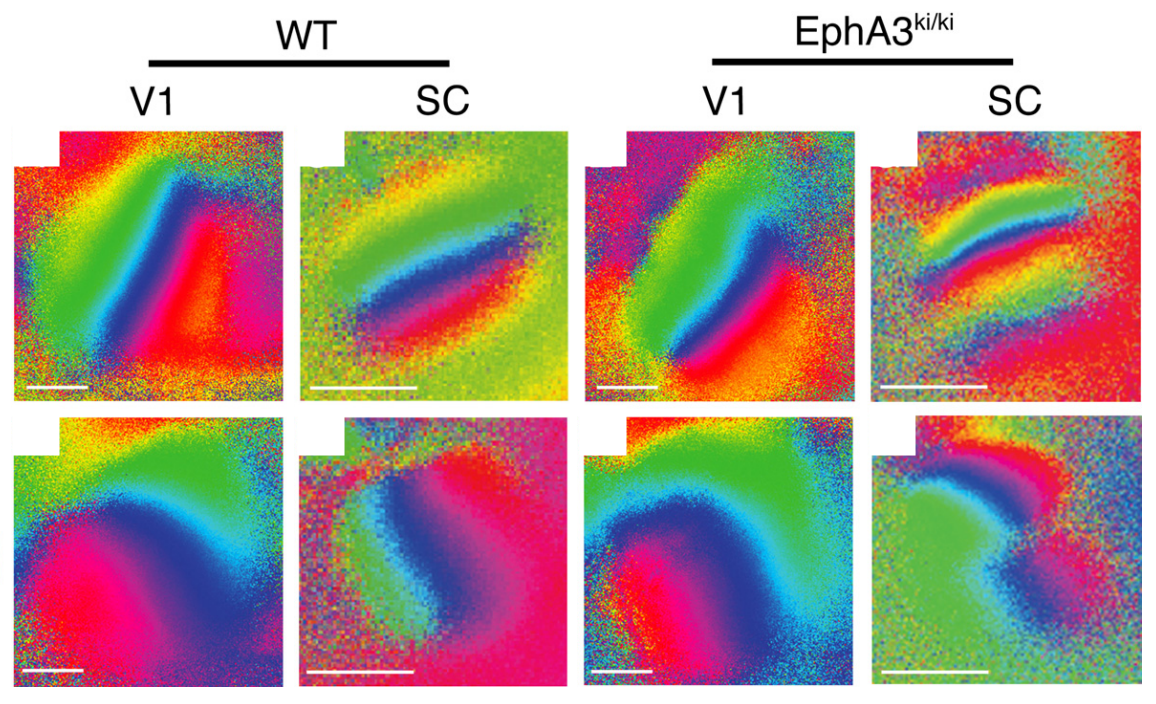
\includegraphics[width = \textwidth]{images/introduction/epha3hom}
		\caption{}
	\end{subfigure}
~
	\begin{subfigure}{0.375\textwidth}
		\centering
		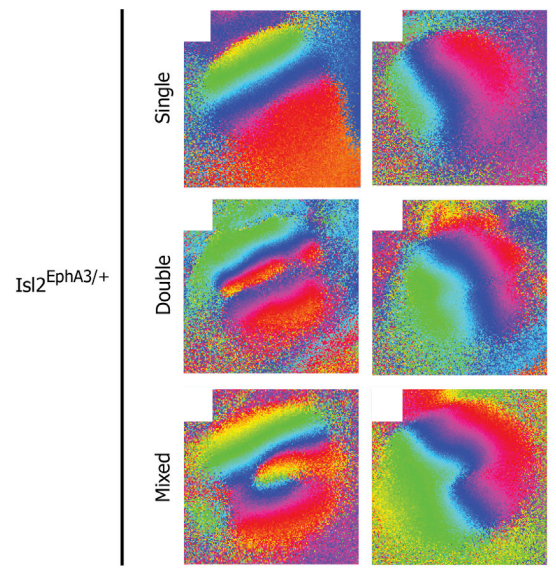
\includegraphics[width = \textwidth]{images/introduction/epha3het}
		\caption{}
	\end{subfigure}
	\def\c{Intrinsic optical imaging scans of EphA3 knock-in mice. }
	\caption[\c]{\label{fig:epha3functional} \c A functional map of the wild-type and the homozygous EphA3 knock-in is presented in the left panel (a). Both maps show functional continuity and a near complete representation of visual space but strikingly the EphA3 knock-in has two such representations completely contained in posterior and anterior regions. The duplication only occurs along the AP axis and the map is singular in the DV axis. Shown here are both the superior colliculus and V1 and interestingly V1 does not present this duplication. Figure adapted from \cite{Triplett2009-si}. \\\\
	The heterozygote maps also have a representation of functional space but they are more varied and less ordered. These maps appear to occasionally present a complete duplication of visual space like a homozygote, occasionally a single representation like a wild-type, and occasionally something in between labelled here as ``mixed". Further analysis on these variants is required.  Figure adapted from \cite{Owens2015-zv}.}
\end{figure}
\FloatBarrier
\subsection{Neural Activity}
The organisation of synaptic connections via activity driven plasticity has notionally existed in the literature since at least the introduction of the chemo-affinity hypothesis as an alternative theory to chemotactic based wiring \cite{Chung1974-oy}. It is difficult to summarise the basic principles of organisation without reference to a computational or mathematical model but it is postulated that a topographic map can be formed by modifying (or creating) a set of synapses with a Hebbian rule and an abstract form of neural activity in the pre-synaptic and post-synaptic regions. The Hebbian rule  states that neurons that are persistently co-active will form synapses such that the potentiation of one leads to the potentiation of another \cite{Abbott2000-gl}. It appears that the activity does indeed propagate forward from the retina into the SC and is spatiotemporally correlated \cite{Ackman2012-uu}.

\subsubsection{Three Periods of Distinct Waves}
There appear to be three periods in which distinct retinal wave types occur in mice \cite{Bansal2000-ts}. The first period occurs at E16-P0 and is characterised by broad wavelengths and small clusters that do not fan out. The second period occurs from P0-P11 and is characterised by only broad fast-moving waves that originate apparently stochastically and spread out over significant portions of the retina; see Figure \ref{fig:wtwaves} \cite{Ackman2012-uu, Stafford2009, Bansal2000-ts}. The final stage occurs very late in development around P11-14 and is characterised by slow but highly localised waves \cite{Bansal2000-ts}.
\begin{figure}
	\centering
	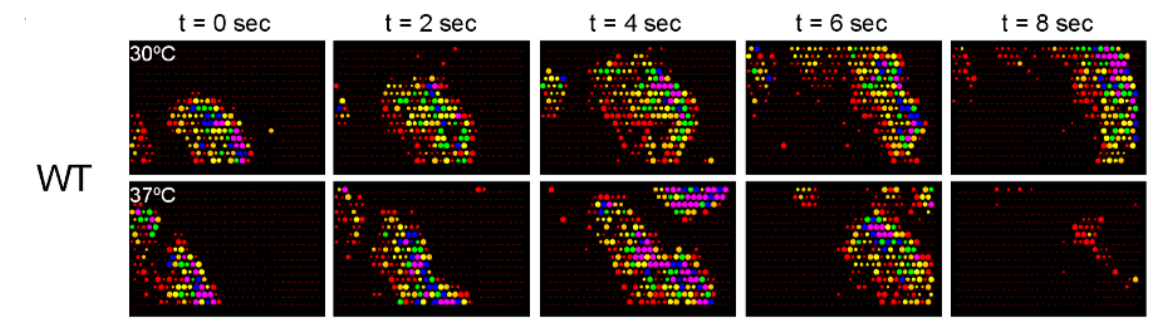
\includegraphics[width = \textwidth]{images/introduction/meaWaves}
	\def\c{Transient snapshots from the retina of a mouse placed on an MEA recorded at P6; the firing note is denoted by colour. }
	\caption[\c]{\label{fig:wtwaves} \c The waves are highly structured and propagate across the retina with the highest firing rates typically at the crest of the wave front. Figure adapted from Stafford et. al. (2009) \cite{Stafford2009}.}
\end{figure}
\subsubsection{$\beta2$  Knock-Out}
A genetic line of mouse has been generated which lacks the nicotinic-acetylcholine receptor $\beta2$ which shall henceforth be referred to as $\beta2$ knockout or just $\beta2^{-/-}$. The effect of the knock-out is a modification of the spatio-temporal characteristics of the waves. Initially it was thought to completely suppress activity leading to a low-correlation between any two given cells \cite{McLaughlin2003-yy}. This turned out to be a temperature based artefact and experiments confirm that it actually generates very fast spreading waves leading to a hyper-correlation between any two given retinal cells \cite{Stafford2009}; see Figure \ref{fig:beta2mea}. The effect of the $\beta2^{-/-}$ is to reduce the precision of the resulting topographic map: the receptive field of a given SC location is large with respect to wild-type \cite{Mrsic-Flogel2005-xp, McLaughlin2003-yy, Chandrasekaran2005-ug}.
\begin{figure}
	\begin{subfigure}{0.6\textwidth}
		\centering
		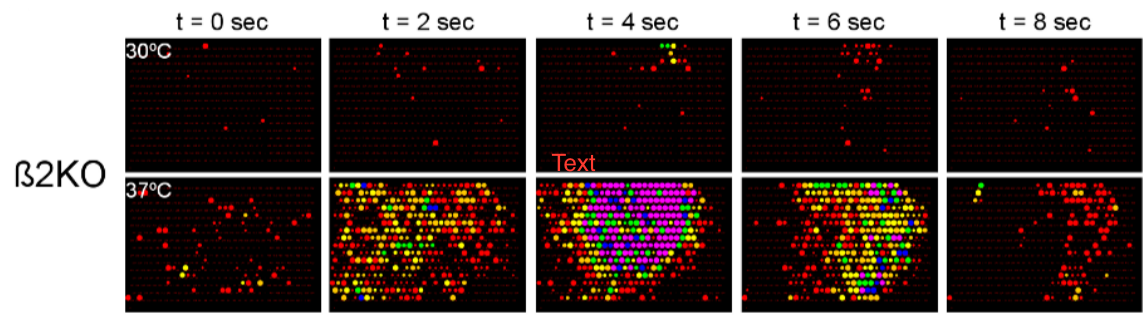
\includegraphics[width = \textwidth]{images/introduction/meaBeta2}
	\end{subfigure}
	~
	\begin{subfigure}{ 0.4\textwidth}
		\centering
		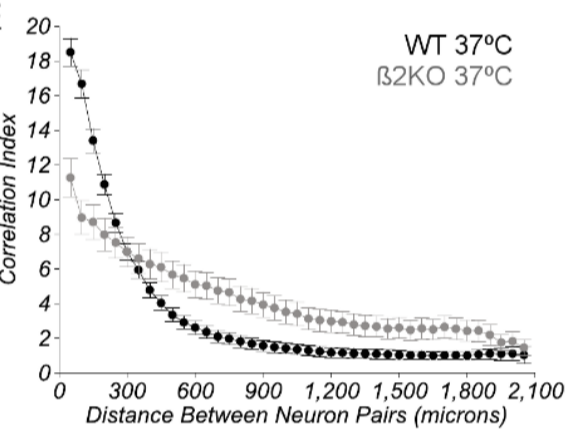
\includegraphics[width = \textwidth]{images/introduction/betacorrelation}
	\end{subfigure}

	\def\c{MEA recordings and correlational profile of retinal waves in the $\beta2^{-/-}$ mouse. }
	\caption[\c]{\label{fig:beta2mea} Transient snapshots from the retina of a $\beta2^{-/-}$ knock-out mouse placed on an MEA and recorded at P6 are shown in the left panel (a). The waves at normal body temperature are highly structured and propagate across the retina quickly and at high firing rates indicating a strong correlation between distal retinal locations. There is barely any activity at a cool temperature of 30C. Figure adapted from Stafford et. al. (2009) \cite{Stafford2009}.
	\\\\
	A measure of correlation is calculated as a function of distance and displayed in the right panel (b). The correlation is strongest for close wild-type pairs and drops off exponentially with a small length scale. For $\beta2^{-/-}$ knock-outs the correlation appears have a longer length scale indicating a hyper-correlation between distant retinal pairs.}
\end{figure}

\subsection{$Math5^{-/-}$ mutant}
The afferent incoming neurons are densely packed necessitating local interaction. They can interact directly with each other via chemical signalling, electrical signalling, or mechanical signalling. They indirectly interact by placing demands on the physical target structure such as metabolic demands of supporting dendritic contacts or physical space constraints. The role of competitive sorting is alluded to by the EphA3 knock-ins which are thought to separate their projections on the basis of relative sorting for which they need to competitively interact \cite{Reber2004-wq, Brown2000-da}. 

The aggregate effects of competitive interactions can be more directly deduced by reducing the number of interacting elements and this was examined in the $Math5$ knock-down \cite{Triplett2011-jk}. The effect of the knock-down was to reduce the number of RGCs born by 95\% distributed randomly across the retina. The substantially reduced number of incoming contacts resulted in a projection isolated to the anterior-medial region of the colliculus; see Figure \ref{fig:math5}.

\begin{figure}
	\centering
	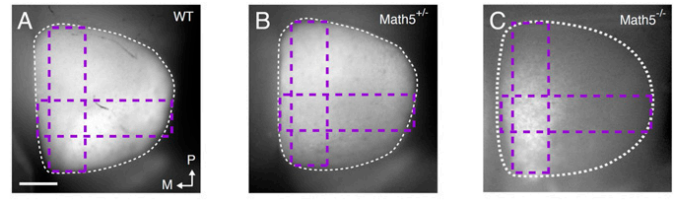
\includegraphics[width = 0.9\textwidth]{images/introduction/math5}
	\def\c{A full retina DiI injection revealing the entire image of the retinal projection on the SC. }
	\caption[\c]{\label{fig:math5} \c The wild-type and $Math5$ single knock-out (A and B) have normal RGC expression. The $Math5$ double knock-out supresses 95\% of RGC cells and subsequently only fills a portion of the anterior-medial colliculus (C). It is important to note that these studies do not show any topographic ordering as the entire colliculus is flooded with the tracer injections. Figure adapted from Triplett et. al. (2011) \cite{Triplett2011-jk}.}
\end{figure}

\FloatBarrier
\section{Developmental Theory  \label{section:developmentaltheory}}
Theoretical considerations have been useful and informative in guiding experimental work on the retinotopic projection with its successful implementation being attributed to a plurality of models and hypotheses guiding and clarifying experimental results \cite{Goodhill2018-ca}. The modelling literature will be examined shortly but the above data can be summarised into the unifying of three historical developmental narratives: the chemo-affinity hypothesis, the activity driven hypothesis, and the competitive sorting hypothesis.

\subsection{Competitive Hypothesis}
The competitive sorting hypothesis is, in essence, very simple working on the assumption that a specific location in the target area can only support a certain amount of synaptic contacts. Each retinal afferent is assumed to have some ability to compete for desirable space in the target area and the ability to compete is graded in some fashion: two common hypotheses were monotonically increasing chemical labels across the dimensions of the retina and time-of-arrival \cite{Prestige1975-vh, jacobson1960studies, Gaze1960-hw}. While evidence suggests chemically graded matching is the true mechanism, time-of-arrival allows discussion of competition without reference to an already discussed developmental mechanism. It states that each retinal point has a distinct location from which it departs and a unique time of arrival based on its time of neurogenesis. The first to arrive will be the first to place contacts and out-compete other incoming retinal afferents. Therefore, a smooth neighbourhood preserving map is formed by temporal differences in arrival of afferents related to the geometric distances between them. Thus, topography is established. This method of establishing topography is extremely sensitive to perturbation; any disruption in the initial ordering will lead to a disruption in the map. These considerations imply that competition with some biasing signal can provide a sorting method to establish topography and which is robust with a persistent bias, as is the case with chemotactic cues, and unstable with a non-persistent bias, such as time-of-arrival.
\subsection{Chemo-affinity Hypothesis \label{section:chemohypothesis}}
The chemo-affinity hypothesis was first proposed by Sperry and is essentially summarised as a mass-action rule: the position of an incoming afferent will be where the equilibrium point of repulsive or attractive chemical forces exists in the post-synaptic target \cite{Sperry1963-jc}. With a monotonic graded chemical distribution in both the pre-synaptic and post-synaptic areas this equilibrium point was proposed to be unique enabling topographic mapping. There is an immediate problem with the initial theory in that if both the pre-synaptic and post-synaptic targets have only one gradient then there is no native equilibrium point. This can be resolved in the first instance by tacitly introducing competitive mechanisms: each afferent will attempt to migrate towards the boundary but those expressing the highest levels of chemical guidance cue will dominate the boundary first with successively lower expression levels occupying successively interior points until a graded match is formed. This has been referred to as a Type I or graded matching mechanism \cite{Hjorth2015-le}. An alternative mechanism would be to introduce a counter-gradient in both directions with opposing interactions thereby establishing a natural equilibrium point where the two forces balance. This has been referred to as a Type II or `lock-and-key' mechanism \cite{Hjorth2015-le}. This mechanism only establishes a smoothly graded topographic map in the target area when the gradients are perfectly matched \cite{Gierer1983-rm, Sterratt2013-ev}. It can be rectified by again introducing competitive mechanisms but in this instance on the target area itself; when each location in the target can only support a given number of synaptic contacts any slight mismatch in gradients will be normalised out \cite{Sterratt2013-ev, Prestige1975-vh}.

\subsection{Activity Driven Hypothesis}
The activity hypothesis is based largely on the Hebbian hypothesis of synaptic potentiation. Briefly, it states that neurons in the pre-synaptic target which have highly correlated patterns of firing activity in the post-synaptic target will increase the strength of the synapses between them \cite{Hebb1949-wr}. Conversely, if these patterns are anti-correlated the synaptic strength will be decreased and thus, a feed-back loop is established. This allows for the \textit{de novo} establishment of topography under the assumption of correlated driving activity in the pre-synaptic area; domains of dominance will naturally be established and these will be continuous by construction. Therefore, a mapping is created with the neighbourhood preserving property and thus topography is established. The major problem with this theory is that when postulated in integral form (as the Hebbian rule is largely assumed to operate) it is valid on domains almost everywhere i.e. there is a set of Lebesgue measure zero (1D) for which discontinuities are allowed. This has significant implications for biology as on this set of discontinuities the orientation of the map can be reversed. This problem, again, can be fixed by including a competitive mechanism. A complete orientation flip would imply that incoming afferents completely cross over each other at least as many times as there are discontinuities which is metabolically costly and physically demanding. If the afferents have to interact with each other they will favour aligned domains and if each individual domain is aligned then they will be continuous across the whole boundary thus establishing topography.

\subsection{Unified Mechanisms}
Each of these three broad mechanisms enjoy experimental support. The existence of the Eph-ephrin class of molecules with a gradient and counter-gradient along both axes strongly implies a chemotactic component with a Type II mechanism. The existence of a series of retinal waves which appear to encode natural visual-field statistics supports the notion of activity driving mechanisms. The effect of the $Math5$ knock-down shows that competitive interaction is essential lending support to all three.

The existence of competition is explained immediately as a corrective mechanism: it alone is too sensitive to random fluctuations to be a primary mechanism but in conjunction with either of the mechanisms it can correct perturbations and sensitivities. Bidirectional chemotaxis with competition seems to be a complete explanation but theoretical considerations about thermal noise and the ability of neurons to detect these molecules means that there is a limit to the precision of the map established \cite{Goodhill2016-ck}. Activity with competition can create a topographic map but it is completely degenerate with respect to rotational symmetry. Therefore, it cannot be relied on to establish a map with a given orientation which is essential when multiple maps need to coordinate inputs. It can however, be relied on to produce precise and well defined domains thus normalising projective/receptive fields at a given width defined by activity patterns. 

These consideration lead to the following explanation: the chemotactic mechanisms in conjunction with competition can establish a well oriented topographic map but are sensitive to a noise floor while detecting relative expression levels of Ephs and ephrins. This explains the large axonal arbours which are initially established in the target. The lock and key nature can be seen in the ephrinA knock-outs which disrupt location specific topographic order. The gradients are also not perfectly matched. In the data this is presented with the axonal overshoot as all afferents compete to reach the preferential boundary. It is further confirmed by the $Math5$ knock-down where only the region near the preferential boundary is occupied suggesting dominance of the gradient or counter-gradient. The activity mechanism is then used to prune the pre-established axonal arbours to a precision that is appropriate to the biological system by matching relevant visual field statistics with a pre-determined spontaneous activity input prior to eye opening.

     
\chapter{Topographic Maps: Mathematical and Computational Modelling \label{chapter:review}}
This chapter will detail some fundamental mathematical theory, techniques for minimisations, discussion about the theory of retinotopic mapping and applications to more general optimisations problems such as the Travelling Salesman Problem, a review of existing models and their limitations, and the research questions which this thesis will address.
\section{Fundamental Mathematics}
Some useful mathematical results, definitions, and standard computational procedures used throughout the text will be covered before discussing details of modelling retinotopic systems. These shall be discussed in general and without formal proof. There are several foundational texts recommended for further discussion \cite{Korner1988-wt, Gelfand2000-xr, Ablowitz2003-iv, Goodfellow-et-al-2016}.
\subsection{Fourier Transform}
The Fourier transform is useful analysis tool which transforms a function into its frequency domain. This thesis will use the following definition of the Fourier transform $\hat{f}(k)$ of a function $f(x)$:
\begin{equation}
\hat{f}(k) = \frac{1}{\sqrt{2 \pi}} \int_{-\infty}^{\infty} e^{-i kx} f(x) dx
\end{equation}
with the inverse transform mapping back from the frequency domain being defined as:
\begin{equation}
f(x) = \frac{1}{\sqrt{2 \pi}} \int_{-\infty}^{\infty} e^{i kx} \hat{f}(k) dk.
\end{equation}
The operation is linear following from the linearity of integration allowing it to be distributed over functions which are compositions of functions. The transform is real if and only if the function on which it operates is a linear combination of even functions and analogously is imaginary if and only if the function is a linear combination of odd functions. The Fourier transform has several elegant algebraic properties which make it useful in differential equation analysis and for evaluating certain integrals.
\paragraph{Fourier Phase Shifting Property}
The Fourier shifting theorem relates the phase of a function to a rotation in the complex plane. The theorem statement is simply:
\begin{equation}
\mathcal{F}[f(x + \phi)] = e^{i \phi}\hat{f}(k).
\end{equation}

\paragraph{Fourier Scaling Property}
The Fourier transform is scaled in a straightforward manner:
\begin{equation}
\mathcal{F}[f(a x)] = \frac{1}{|c|}\hat{f}(\frac{k}{c}).
\end{equation}
\subsubsection{Fourier Convolution Theorem}
The Fourier convolution theorem allows for convolutions of functions to be decomposed into their products in Fourier space. It is stated as:
\begin{equation}
\mathcal{F}[(f\star g)(x)](k) = \sqrt{2 \pi}\hat{f}(k) \hat{g}(k),
\end{equation}
where $\star$ denotes the convolution operator: $(f \star g)(x) = \int_{-\infty}^{\infty} f(x-\xi)g(\xi) d \xi$.

\paragraph{Fourier Differentiation Operator}
The Fourier transform allows derivatives to be transformed into polynomial expressions:
\begin{equation}
\mathcal{F}\left[\frac{d^n}{dx^n}f(x)\right](k) = (ik)^n \hat{f}(k).
\end{equation}
\subsection{Cauchy's Residue Theorem}
Cauchy's Residue Theorem is an elegant statement in complex analysis which allows the evaluation of a closed line integral to be evaluated by only summing its residues which are typically relatively simple to calculate. First, the Laurent series of a function $f$ around the point $c$ is defined as:
\begin{equation}
f(x) = \sum_{n=-\infty}^{n=\infty} a_n(x - c)^n,
\end{equation}
where the coefficients $a_n$ are given by an expression which generalises Cauchy's integral formula. The residue of $f$ is given by $a_{-1}$. Consider a region of the complex plane $U$ enclosed by a simple curve $\gamma$ and suppose that a function $f$ has singularities at $\{A_1, ..., A_k\}$ and is analytic at all other points in $U$. By the residue theorem the counter-clockwise line integral of $f$ around $\gamma$ is evaluated as:
\begin{equation}
\ointctrclockwise_\gamma f(x) dx = 2 \pi \sum_{i = 0} ^{k} \text{Res}(f, A_i),
\end{equation}
where $\text{Res}(f, A_i)$ is the residue of $f$ evaluated at $x = A_i$. This result allows for several otherwise complicated integrals to be evaluated.
\subsection{Variational Calculus}
A functional is a mapping from the space of all functions to the real line. Variational calculus typically examines how a functional varies with respect to functions. Analogously to traditional calculus special attention is paid to extrema of the functional which are found by minimising the first variation which is analogous to the first derivative. Suppose that $E$ is a functional and let $y(x)$ be some function and $h(x)$ be some small change to $y(x)$ the change in the functional is accordingly:
\begin{equation}
\Delta E = E[y + h] - E[y].
\end{equation}
The functional is said to be differentiable when there exists a linear functional $\kappa_1$ and $\epsilon >0$ such that $\epsilon \rightarrow 0$ when $\lVert h \rVert \rightarrow 0$ and:
\begin{equation}
\Delta E[h] = \kappa_1[h] + \epsilon  \lVert h \rVert.
\end{equation}
The functional $\kappa_1[h]$ is the first variation of $E$ at function $y$ and is denoted as $\delta E / \delta y$. The second variation  $\delta^2 E / \delta y^2$is accordingly defined by the linear functional $\kappa_2$ if the following exists such that $\epsilon \rightarrow 0$ when $\lVert h \rVert \rightarrow 0$:
\begin{equation}
\Delta E[h] = \kappa_1[h] + \kappa_2[h] + \epsilon  \lVert h \rVert^2.
\end{equation}
If there exists $k>0$ such that $\kappa_2[h] > k  \lVert h \rVert^2$ then the second variation is said to be strongly positive. A sufficient condition for $y$ to be a minimum of the functional $E$ is that the first variation of $E$ at $y$ is 0 and that the second variation at $y$ is strongly positive. 

Functionals are often defined by an integral of an abstract algebraic expression $L$ of the function ($y$), its derivative ($y^\prime$), and the function variable ($x$):
\begin{equation}
E[y] = \int_{x=a}^{x=b} L(y, y^\prime, x)dx
\end{equation}

\subsection{Euler-Lagrange Equations}
The process of finding minima of a functional typically involves solving the Euler Lagrange equations which are derived as follows. Assume the function takes a minima at $\hat{y}$ and define an arbitrary function $\eta(x)$ such that $\eta(a)=\eta(b)=0$ and $\eta^\prime(x)$ exists and is not 0. Then, for sufficiently small $\epsilon$ the first variation is $\epsilon\eta(x)$. Substituting $y(x) = f(x) + \epsilon \eta(x)$ the functional can be considered as a function $\Phi(\epsilon)$ which takes a minimum at $\epsilon = 0$ which immediately implies $\Phi^\prime(0) = 0$. Taking the total derivative $dL/d\epsilon$ and evaluating at $\epsilon = 0$ minimises the first variation and thus gives necessary conditions for $f$ the minima. Expanding the derivative, integrating by parts, and evaluating $\eta(x)$ at the boundary leads to:
\begin{equation}
\int_{x=a}^{x=b} \left.\frac{dL(y, \dot{y}, x)}{d\epsilon}\right\vert_{\epsilon = 0} dx = \int_{x=a}^{x=b} \eta(x)\left( \frac{dL}{df} -  \frac{d}{dx}\left(\frac{dL}{df^\prime}\right)\right)dx
\end{equation}
Then, $\Phi^\prime(0) = 0$ implies that this must be equal to 0 and the Fundamental Lemma of Variational Calculus is applied which states that an integral of a product of some function $f$ with any smooth compactly supported function over a domain is zero if and only if $f = 0$ over the domain. This leads to the Euler-Lagrange equations:
\begin{equation}
\frac{dL}{df} - \frac{d}{dx}\left(\frac{dL}{df^\prime}\right) = 0 
\end{equation}
These are typically a set of second order differential equations which can be solved by standard means using appropriate boundary conditions.
\subsection{Numerical Minimisation \label{sec:minimisation}} 
Often the Euler-Lagrange equations, while derivable, are not easily solved analytically. In these instances a numerical optimisation scheme can be used by choosing some starting function $f_0(x, t)$ and advancing $t$ using the partial differential equation:
\begin{equation}
\frac{dL}{df} - \frac{d}{dx}\left(\frac{dL}{df^\prime}\right) = \frac{\partial f}{\partial t}.
\end{equation}
The procedure follows by consideration of the minimisation of $\Phi$ and will then find a location for which there is a \textit{local} minima but there is no guarantee that the functional is totally minimised. Any numeric optimisation scheme can be used to advance $f$ until $\partial f / \partial t= 0$.
\subsection{Optimisation}
The process of finding extrema (minima/maxima) points for a function is known as optimisation and is an active research area of applied mathematics. There is no general method for finding a global extrema unless the space is discrete in which case it may be found by enumeration. However, discrete problems often scale as factorials rendering direct computation infeasible and it is often desirable to use non-guaranteed methodologies either directly or by embedding the problem in continuous space. 
\subsubsection{Gradient Descent} \label{sec:graddescent}
Gradient descent is an efficient minimisation scheme that works particularly well on convex functions. It assumes that the function to be minimized, $f(\vec{x})$ where $\vec{x} \in \mathbb{R}^n$, has a well defined gradient at all points in the search space $S$. It follows from elementary vector calculus that $\nabla_{\vec{x}} f(\vec{x})$ is a vector oriented along the direction of greatest local increase of the function $f$. The gradient descent routine is relatively simple and is parametrised by a single value $\epsilon > 0$ which is often referred to as the learning rate. An initial point in the search space $\vec{x}_0 \in S$ is chosen and the following update rule is applied:
\begin{equation}
\vec{x}_{t+1} = \vec{x}_t - \epsilon \nabla_{\vec{x}} f(\vec{x}).
\end{equation}
\paragraph{Convergence}
The update is applied for an arbitrary amount of timesteps $T$ or until a point $\vec{x}_{t}$ is reached such that $\nabla_{\vec{x_t}} f(\vec{x_t}) = 0$ whichever comes first. In the second case the solution will have converged to a local extrema in the search space and it will not escape this extrema. The extrema can theoretically be a minima, maxima, or saddle point as these would all result in a zero gradient but unless initialised precisely on a maxima it will be either a saddle or minima. A saddle point will be numerically unstable in at least one direction and therefore any small perturbations, perhaps introduced by a numerical instability, will result in the algorithm moving along this direction and away from the point. Therefore, a stable convergence typically implies that a local minima has been found. In the first case the value $f(x_T)$ will be necessarily lower than $f(x_0)$ but it will not necessarily be a minima.
\paragraph{Issues}
Gradient descent converges slowly making it unfeasible to use on large problems and problems which present a large variation of steepness in the gradient landscape. A gradient descent algorithm will slow down in a relatively flat landscape necessitating a large learning rate $\epsilon$ or an arbitrarily long computation time. Likewise, if the landscape is steep then a large $\epsilon$ will result in an overshoot of the minima and force an oscillatory solution. Therefore, the learning rate should be tuned to match the expected steepness of the function as well as ensuring reasonable convergence time. However, the steepness of the function cannot be known \textit{a priori} and an arbitrary function will generally present a range of gradient magnitudes making the choice of $\epsilon$ difficult. Furthermore, a gradient descent algorithm will converge to the most proximal local minima, and while this is often sufficient for the optimisation task, it has no guarantees on being the optimal minima and for complicated functions with many local minima it is almost certainly not the optimal.
\subsubsection{Generalised Momentum Rules}
To improve the gradient descent algorithm the idea of momentum was introduced --- a component of the previous update is maintained and incorporated into the current update \cite{Polyak1964-bt}. The relative component of the previous update is specified by a second hyper-parameter $\alpha$. Letting $v_t$ denote the update at timestep $t$ the rule is given by:
\begin{align}
\vec{u}_{t+1} &= \alpha \vec{u}_t - \eta \nabla_{\vec{x}} f(\vec{x}) \\
\vec{x}_{t+1} &= \vec{x}_t + \vec{u}_{t+1}.
\end{align}
The above rule may be generalised to allow for the update to be computed as an arbitrary function $g$ of the function variables, gradient, the previous update, and a set of associated hyper parameters $\vec{P}$ ; of course it may be more general even still but these choices are most common. The update rule then becomes:
\begin{align}
u_{t+1} &= g(\vec{x}_t, \vec{u}_t, \nabla_{\vec{x}} f(\vec{x}; \vec{P})) \\
x_{t+1} &= \vec{x}_t + \vec{u}_{t+1}.
\end{align}
Determining the form of $g$ and tuning the hyper-parameters $\vec{P}$ is an active area of research, particularly in the machine learning community. There have been several proposed candidates for $g$ which are typically generated by consideration of a single problem or dataset and then become notable when they are found to generalise. Such routines include: Nesterov Descent, RMSPROP, ADAM, NADAM, ADAMAX \cite{Sutskever2013-ng, Dozat2016-dj, kingma2017adam}. The convergence guarantees are the same as for regular momentum in the asymptotic limit but in practice they are often found to converge more rapidly and stably than the vanilla routine. However, there is an active debate about their generality with many authors arguing that (stochastic) gradient descent is a better general optimiser. Nevertheless, they are important and often powerful techniques for optimisation.
\paragraph{ADAM}
A particular routine that was developed originally for the classification of images but has been adopted widely is the adaptive moment routine ADAM which aims to tune its learning rate dynamically throughout the descent. The routine relies on the computation of the secondary moments of the curvature in the gradient landscape and very efficiently finds a near optimal minima. The equations that define it are specified by:
\begin{align}
&m_{t+1} = \beta_1 \vec{m}_t + (1 - \beta_1) \nabla_{\vec{x}} f(\vec{x})\\
&\vec{v}_{t+1} = \beta_2 \vec{v}_t + (1 - \beta_1) (\nabla_{\vec{x}} f(\vec{x}))^2\\
& \vec{u}_{t+1} = -\eta \frac{\vec{m}_{t+1}}{(1+\beta_1^t)\left(\sqrt{\frac{\vec{v}_{t+1}}{1+\beta_2^t}} + \epsilon\right)}\\
& \vec{x}_{t+1} = \vec{x}_t + \vec{u}_{t+1},
\end{align}
where $\epsilon \ll 1$ is some small constant to avoid a division by zero error, $\beta_1$ and $\beta2$ are the adaptive momentum hyper-parameters, and $\eta$ is the learning rate.
\begin{figure}[h!]
	\centering
	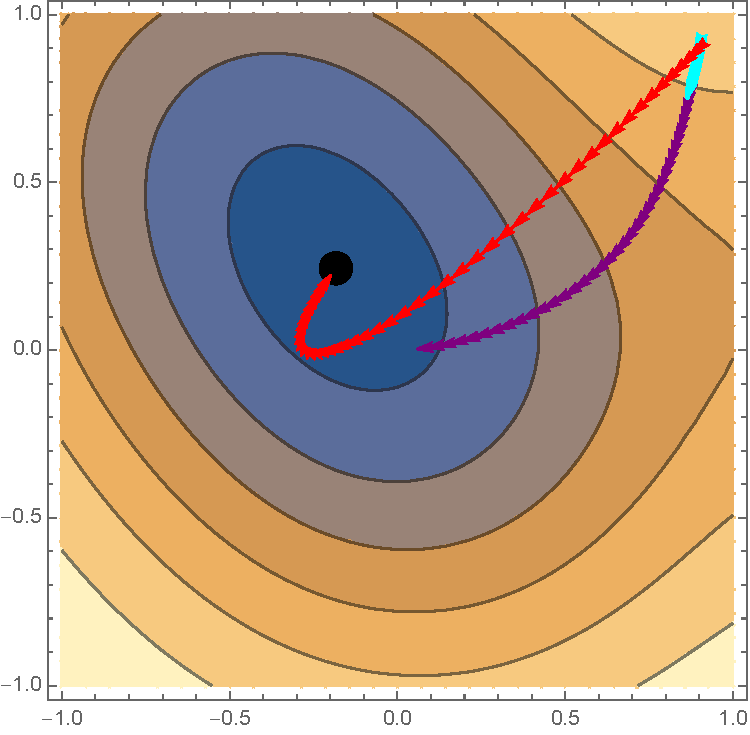
\includegraphics[width = 0.67\textwidth]{images/introduction/momentum}
	\def\c{Gradient descent routines using vanilla gradient descent (cyan), momentum (purple), and ADAM (red)}
	\caption[\c]{\c. Each routine was initialised at the same location in the top right corner of the search space and the energy function being optimised increases in value from blue to yellow. The learning rate was set to $\eta = 0.005$ and the hyper-parameters where left at their defaults $\beta_1 = 0.9, \beta_2 = 0.999$. The algorithm was ran for 100 steps and the minimum is found at the centre of the black disk. At each step the position and corresponding update step is plotted as a coloured vector. While momentum is a vast improvement on vanilla gradient descent it is outperformed by ADAM which takes a more direct line and converges more quickly. \label{fig:momemtum}} 
\end{figure}
\subsubsection{Simulated Annealing}
Simulated annealing is a heuristic non-linear optimiser that has its roots in simulating the process of a metal cooling \cite{William_H_Press2007-kb}. It works by allowing probabilistic jumps in the solution space which depend on the simulated temperature at a given time step. Suppose that $f$ is a function parametrised by $\vec{x} \in \mathbb{R}^n$ and the task is to minimise $f(\vec{x})$. An initial temperature $K$ is chosen and an annealing schedule such that for each timestep $K_t \mapsto K_0 / t$ where $\alpha \in (0, 1)$. Then, at each timestep a new parameter $\vec{x}^*$ is proposed in some appropriate neighbour set $S \subseteq \mathbb{R}^n$ which can potentially be the whole space. At each timestep the transition probability $p_t$ is calculated:
\begin{equation}
p_t = \exp\left(-\frac{f(\vec{x}^*)- f(\vec{x})}{K_t}\right).
\end{equation}
A random number $p_\alpha$ is uniformly sampled between $[0, 1]$ and if $p_\alpha < p_t$ the proposed state change is accepted. Note that any state change that results in a reduction of $f$ will be automatically accepted when $p_t > 1$. However, a change that increases $f$ may still be probabilistically accepted. While this seems counter-intuitive as an increase in $f$ moves the algorithm further away from the optimisation goal, it is useful for sampling the search space widely and allows the algorithm to more frequently break out of local minima which gradient descent algorithms may be trapped in. Finally, a trace of all available states is kept and the state that minimises $f$ is selected as the optima. 

\section{Modelling of Retinotopic Maps \label{sec:models}}
The modelling of retinotopic development has a long history with several hundreds of instances of models appearing in the literature. Models in this field are primarily data-driven and aim to explain one or mechanisms of an observed biological phenomenon. In this fashion they are tightly coupled to, and often drivers of, hypothesis driven experimental research with an observation by Goodhill reading: 
\begin{displaycquote}{Goodhill2018-ca}
Starting with Sperry’s chemospecificity hypothesis and the resulting search for molecules that might implement this, retinotectal map formation is an area where theoretical ideas have been unusually influential on experimental work. Rather than there being one ‘‘correct’’ model, competing theoretical hypotheses have all helped guide and clarify experimental results.
\end{displaycquote}
Early work in the field has been extensively reviewed by Swindale (1996), and then later by Hjorth et. al. (2015) and Gjorgjieva and Eglen (2014) \cite{Swindale1996-kk, Hjorth2015-le, Gjorgjieva2011-de}. The broad classes of mechanistic modelling alongside recent developments and several models that were not included in later reviews are now summarised. First, a comment about stability: a fundamental component of all topographic modelling. Each model is designed to either be natively static, or undergo some iterative process until it becomes so. This iterative process can be interpreted as meaningful and allow for the testing of development hypotheses, or as a convenience just allowing the final map to be generated. In either case it suggests that there is a fundamental minima to be found either as the steady state of a dynamical system, or the action of some Lagrangian (Hamiltonian). This would suggest that an energy formulation is desirable for all models, although it is not guaranteed as there is no general formulation for the inverse problem of Lagrangian mechanics. Furthermore, it is not always helpful to formulate the problem in this manner as many models are defined by computational routines which can be tricky to translate into this framework and these are sometimes best worked with directly. Nevertheless, it provides a useful abstract canvas on which to paint modelling problems. 
Some generalised approaches to modelling the three key mechanisms of competition, chemotaxis, and neural activity discussed previously will now be covered. These general techniques underpin the vast majority of models of topographic development.
\subsection{Competition}
Competition has typically been used to refer to competition for physical space or for metabolic resources and with the exception of some finely tuned chemotaxis models it forms a necessary component of every topographic model. Competition typically relates the rate of change of synaptic density at a location to the synaptic density itself. Letting $w_i(\vec{x}, t)$ represent the density of synapses at location $\vec{x}$ and time $t$ from afferent $i$ in a pool of afferents of size $N$ leads to:
\begin{equation}
\frac{dw_i (\vec{x}, t)}{dt} = f\left(\{w_j (\vec{x}, t) \}_{j=1}^N\right)
\end{equation} 
This is a general formulation but is nevertheless employed e.g. Triplett et. al. (2011) choose a highly non-linear function on both the synapses incumbent on a post-synaptic location and the number of pre-synaptic locations these synapses arrive from \cite{Triplett2011-jk}. Competition is sometimes referred to as normalisation and in these contexts it is typically simple and thought of with two dominant mechanisms: subtractive and multiplicative. Subtractive normalisation is an extreme form of normalisation given by:
\begin{equation}
\frac{dw_i(\vec{x}, t)}{dt} = Q-\alpha \sum_i w_i (\vec{x}, t),
\end{equation} 
where $\alpha$ is some constant and Q is the total weight available to some post-synaptic location \cite{Goodhill1991-fu, Goodhill1993-lk}. To stop the density from becoming negative, a physically impossible situation, one of two things are usually done: hard code a boundary at zero, or sum the total number of synapses in the system and scale it to some constant. Without some other mechanism to promote synaptic growth subtractive normalisation will lead to a rapid decay of contacts typically promoting a winner-take-all environment \cite{Miller1994-nr}. Multiplicative normalisation is given by:
\begin{equation}
\frac{dw_i(\vec{x}, t)}{dt} = -\frac{\alpha w_i(\vec{x}, t)}{g\left(\sum_j w_j(\vec{x}, t)\right)},
\end{equation}
where $\alpha$ is some constant \cite{Kohonen1982-nd, Obermayer1990-yr}. In the absence of growth this leads to an exponential decay in synaptic density between the pre-synaptic and post-synaptic locations and is therefore slower than multiplicative normalisation in the low density regime. Multiplicative normalisation therefore does not typically need a stabilisation mechanism. A natural fixed point emerges in this rule defining the density at which the growth mechanism precisely matches the decay induced by additional synapses.

To introduce competition into an energy based formulation it is sufficient to simply penalise the existence of synaptic contacts i.e. by adding energy in an energy minimisation scheme, or subtracting in a maximisation scheme. A subtractive normalisation can be modelled by associating competitive energy by summing or integrating all contacts in the system and parsing it through some function $f$:
\begin{equation}
E = f\left(\sum_i\int w_i(\vec{x}) \; d\vec{x} \right).
\end{equation}
Analogously, a multiplicative normalisation can be modelled by integrating all local contacts and parsing it through some $f$ and then summing all transformed local contributions:
\begin{equation}
E = \sum_i f\left(\int w_i(\vec{x}) \; d\vec{x}\right).
\end{equation}
\subsection{Chemotaxis \label{sec:chemotaxismodelling}}
Chemotaxis modelling has almost universally converged on two types of model: Type I and Type II  defined in Section \ref{section:chemohypothesis} \cite{Hjorth2015-le}. Both types assume that each retinal afferents affinity to a particular colliculus location is some function of the concentration of ligands and receptors at the location. In Type I systems each retinal afferent has the highest affinity for a single colliculus location but the strength of these affinity's vary. In Type II systems the receptors and ligands encoded by each afferent and each location insist on an optimal target in the colliculus for each afferent. The effect of these interactions is modelled in two general ways: an energy scheme whereby the minimal energy configuration encodes the affinity \cite{Willshaw_D_J1979-eg, Koulakov2004-ia, Tsigankov2006-uy, Tsigankov2010-on, Triplett2011-jk, Gierer1981-qc}, or a differential scheme whereby each afferent moves in accordance with a local measurement of the relevant concentrations \cite{Simpson2011-zh, Sterratt2013-ev, Gierer1983-tn, Willshaw2006-if}:
\begin{align}
E_i =& f\left(\{R^u_s(\vec{x}^u_i), L^u_s(\vec{x}^u_i): u \in \{\text{r}, \text{c}\}, s \in \{A, B\} \}\right)\\
\frac{\partial\vec{x}^\text{c}_i}{\partial_t} =& f\left(\{R^u_s(\vec{x}^u_i), L^u_s(\vec{x}^u_i) : u \in \{\text{r}, \text{c}\}, s \in \{A, B\} \}\right) 
\end{align}
where $i$ denotes the index of the afferent, $r$ and $c$ denote the retina and colliculus, and $R$ and $L$ denote the receptor and ligand concentrations of a particular subsystem respectively. In many cases the two formulations are equivalent but it is not guaranteed. In the case of multiple interacting mechanisms (Type I mechanisms require at least a competitive mechanism), the energy formulation can produce differing results to the differential mechanism depending on either the choice of energy minimisation scheme, or the initialisation location of the afferents. Simple cartoons of both differential and energy affinity maximisation schemes are shown for Type I mechanisms are shown in Figures \ref{fig:affchemotaxistype1} and \ref{fig:diffchemotaxistype1}, and Type II mechanisms are shown in Figures \ref{fig:affchemotaxistype2} and \ref{fig:diffchemotaxistype2}. 

\begin{figure}[h!]
	\centering
	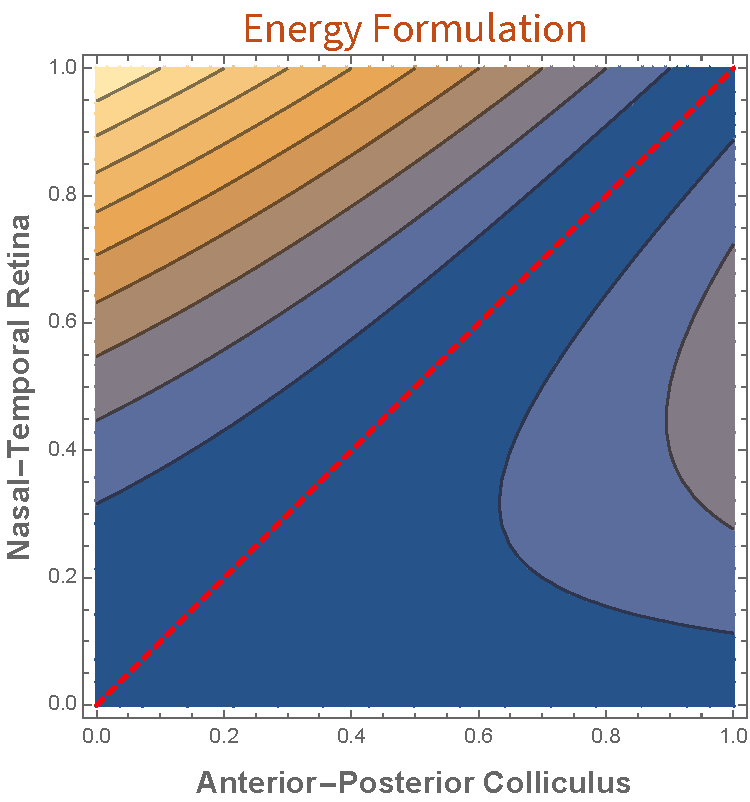
\includegraphics[width=\textwidth]{images/introduction/energy_chemotaxis_type1}
	\def\c{A simple formulation of an energy minimising scheme where the chemotactic affinity is proportional to the product of the retinal and colliculus locations along the NT and AP axes respectively.}
	\caption[\c]{\c Due to the increasing affinity along the AP axes for each retinal site there is assumed to be a competitive penalty scaling with the square of the position vector. The resulting energy profile has a non-linear shape introduced by the gradient product and mimicking the likely biological reality. The zero energy contour is highlighted in red. \label{fig:affchemotaxistype1}} 
\end{figure}

\begin{figure}[h!]
	\centering
	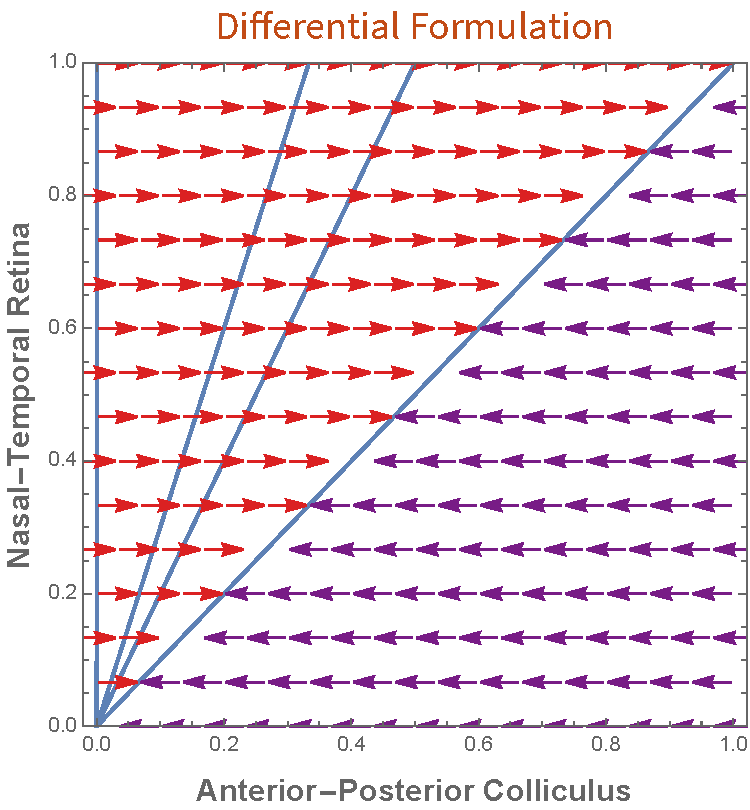
\includegraphics[width=\textwidth]{images/introduction/differential_chemotaxis_type1}
	\def\c{A simple formulation of a differential chemotaxis scheme whereby the axons in the naso-temporal retina move forward at a rate proportional to their starting location. The travelling wave front is represented by the blue fanning lines.}
	\caption[\c]{\c When first axons arrive at the hard barrier they create a barrier applying a repulsive force labelled in purple. Since this repulsive force is mediated by axonal arrival the wave front is halted along the line y=x. \label{fig:diffchemotaxistype1}} 
\end{figure}
\begin{figure}[h!]
	\centering
	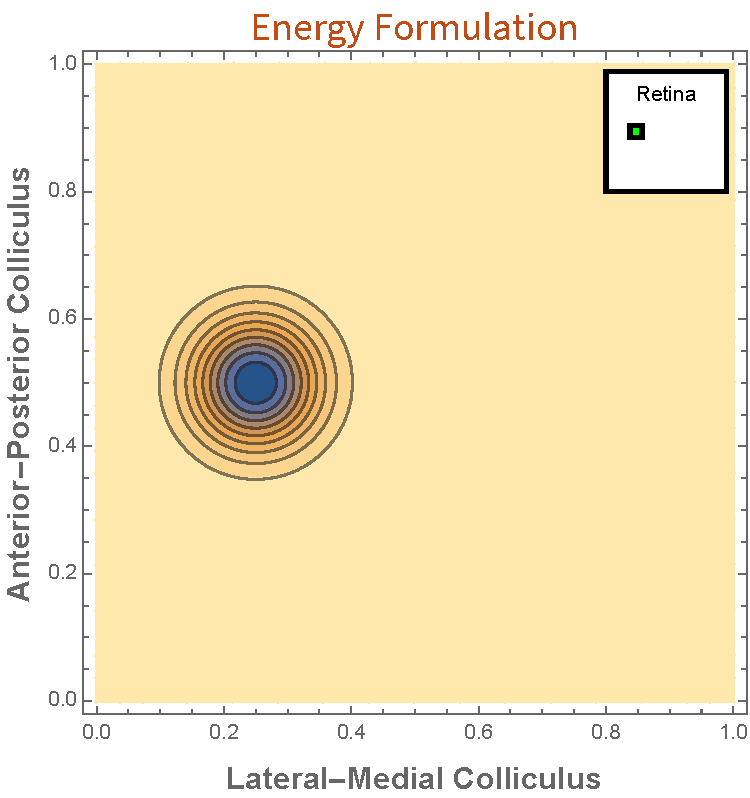
\includegraphics[width=\textwidth]{images/introduction/energy_chemotaxis_type2}
	\def\c{A simple formulation of an affinity chemotaxis scheme where the green label in the retina is given a value of both ligand and receptor. }
	\caption[\c]{\c The entire colliculus target is given a series of ligands and receptors and the quotient of products of ligands with the receptors defines the affinity. Assuming an exponential profile for all receptors and ligands $\exp(|R(\vec{x}^R)L(\vec{x}^C|)/\exp(|R(\vec{x}^C)L(\vec{x}^R)|)$; this formulation is derived from the seminal Geirer model \cite{Gierer1983-tn}.  \label{fig:affchemotaxistype2}} 
\end{figure}
\begin{figure}[h!]
	\centering
	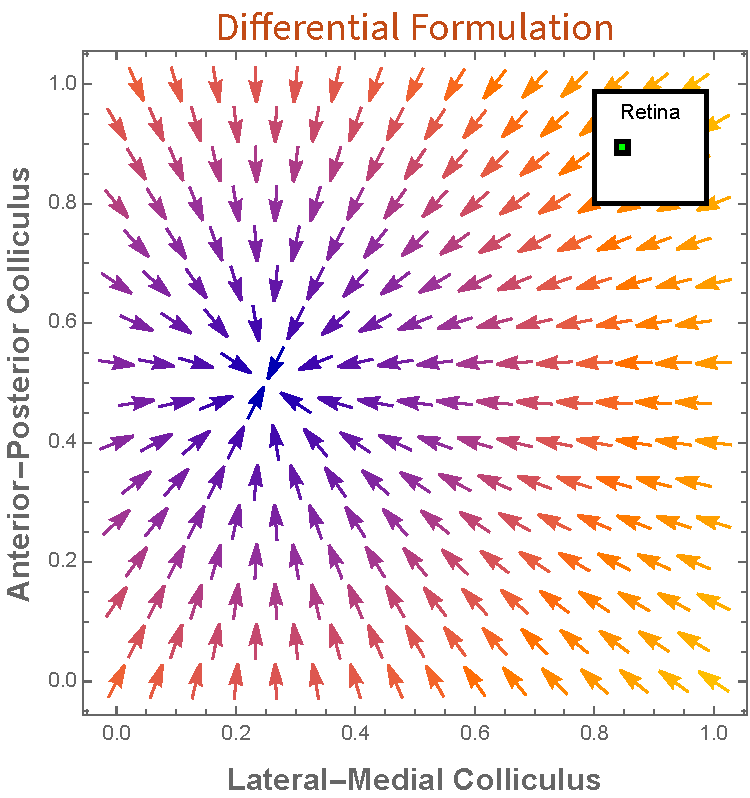
\includegraphics[width=\textwidth]{images/introduction/differential_chemotaxis_type2}
	\def\c{A simple formulation of a differential chemotaxis scheme where the green label in the retina is guided by a series of forces imposed by the interaction of the receptor and ligand values at the retinal location with various location in the target. }
	\caption[\c]{A simple formulation of a differential chemotaxis scheme where the green label in the retina is guided by a series of forces imposed by the interaction of the receptor and ligand values at the retinal location with various location in the target. The force at each location is indicated by a vector and its magnitude by a colour increasing from blue to yellow. The combinations of these forces guide the afferent into a stable location. \label{fig:diffchemotaxistype2}} 
\end{figure}

\paragraph{Fibre-Fibre Interactions}
The above cartoons deal only with fibre-target interactions with vector forces or affinities being largely composed as a result of combinations of a retinal origin position and the afferents position in the target. More complicated interactions would account for nearby afferents positions in the retina allowing for fibre-fibre chemotactic movements. This idea was the basis for the relative signalling model proposed first by Reber (2004) \cite{Reber2004-wq}. In general, models typically do not include these interactions but a more detailed discussion about them was offered by Weth et. al. (2014) \cite{Weth2014-dq}. 
\subsection{Activity \label{sec:activity}}
Chemotaxis and competition are relatively simple to describe mathematically with immediate implications. Conversely, the effects of neuronal activity on the organisation of topography is more complicated and will require detailed discussion of several mechanisms.  Neural activity is a loosely defined term which can refer to any number of collective behaviours. It is usually taken to mean a process by which a set of neurons can signal and modulate behaviour of other neurons within that set. This is most often taken to refer to spiking but several systems exhibit sub-spiking threshold activity. Furthermore, several authors take the position that rather than individual spikes being the relevant quantity it is the spiking rate which encodes relevant information.
\paragraph{Neuronal Spiking}
There are three major classes of model for describing spiking behaviour: biophysical, integrate-and-fire, and Poisson. The biophysical model is typically inspired by the work of Hodgkin and Huxley and is concerned with the non-linear modelling of membrane voltage along a cell body with three response variables \cite{Hodgkin1952-yi}. The Hodgkin-Huxley model has been extensively developed and computational packages such as neuron can model individual compartments of a neuron and its firing in detail \cite{Carnevale2006-gn}. In general, these models are too computationally intensive to apply to large scale studies and will not be detailed further.

A simpler model that captures much of the underlying biophysics is the integrate-and-fire which is desirable for its computational-efficiency to accuracy trade-off \cite{Abbott1999-ms, Burkitt2006-ne}. This class of model typically assumes a membrane potential variable $v_i(t)$ and a response variable $u_i(t)$ and some input $I_i(t)$ at a node $i$, along with a set of threshold parameters $\vec{P}$ which specify the threshold potential at which a spike occurs and what the potential and response variables should be reset to after this spiking event. These models have the general form:
\begin{align}
&\dot{v}_i(t) = f(u, v, I; \vec{P})\\
&\dot{u}_i(t) = g(u, v, I; \vec{P}),
\end{align}
for some general functions $f$ and $g$. The functions can be relatively simple as in the leaky integrate-and-fire neuron where $f(v, I) = \alpha - v + I$ for some constant $\alpha$ and $g = 0$. They can also be relatively complex aiming to capture almost all of the underlying bio-physics while maintaining efficiency; see Izhekvich for a detailed formulation \cite{Izhikevich2003-ht}. 

The simplest model in terms of computational efficiency of spike generation is the Poisson model. In this model a neuron is assumed to have a possibly time-varying firing rate $r(t)$ and for a given time interval $dt$ is assumed to release $r(t) dt$ spikes. The probability of releasing a spike is independent of any spikes that have occurred previously and thus the probability distribution is Poisson. Therefore, a time-series of activity can be generated by partitioning the time into sufficiently many intervals of length $dt$ and for each interval comparing a random number sampled from a uniform distribution with $r(t)dt$: if the random number exceeds $r(t)dt$ then there is no spike and vice-versa. This spiking model, while cheap and relying on simplifying assumptions, has been shown to capture many properties of the underlying neural activity distributions \cite{Burkitt2006-wq, Burkitt2006-ne}.

\paragraph{Neuronal Networks}
A natural extension from these spiking models of neurons is to model portions of the brain as a network of coupled nodes that each exhibit these spiking dynamics. A network in network science is an ordered triple $\mathcal{R}(N,E,f)$ where $N$ is a set of nodes in the network, $E$ is a set of edges and $f$ is a mapping from an edge in $E$ to a pair of nodes in $N$ \cite{Barabasi2016-wx}. 

Networks can be directed or undirected. In a directed network the edges can have a specific direction attached to them so for each pair of nodes $i$ and $j$ there are two possible edges; $f: E \rightarrow N\times N$. Networks can also be weighted or unweighted. In a weighted network a real number is assigned to each edge by a weight function $w: E \rightarrow \mathbb{R}$. All of this information can be contained in a matrix called the adjacency matrix $\mathcal{A}$. The entries of the adjacency matrix $\mathcal{A}_{i,j}$ are given by the weight function of the edge between nodes $i$ and $j$ and are zero if no edge exists between them.

Each node on the network may exhibit some dynamics. Consider a set of parameters $\vec{v}_i$ which describe the dynamics of a node $i$. The dynamics of each node will be dependent on some internal dynamics as well as some input from other nodes which connect to it. If there are $n$ such nodes in the system this can be summarised as:
\begin{equation}
\dot{\vec{v}}_i=F(\vec{v}_i)+\sum_{j=1}^{n} G(\mathcal{A}_{i,j},\vec{v}_i,\vec{v}_j,\dot{\vec{v}}_j).
\end{equation}
The function $F$ determines the effect of the internal dynamics and the function $G$ determines the input of the $j$-th node to the dynamics as a function of the weight of the edge between them, the dynamics of the $j$-th node and the state of the $i$-th node. Solving this equation will completely determine the dynamics of the system. In general there may be no analytical solution to this equation.

A neural network may then be constructed by associating each node with a neuron and each edge with a synaptic connection. For a simple consideration, consider a leaky-integrator model where activity on the $i$-th neuron is given by $u_i$, the time scale of the leak is given by $\tau$, the activation function is given by $f$ and the $j$-th neuron is coupled to the $i$-th with a synaptic weight $w_{ij}$. It is assumed here that a spike in the $j$-th neuron induces a rapid change in the potential of $u_i$ of $w_{ij}$ by the release of neurotransmitters and then this change decays exponentially; a simplistic form of synaptic processing. The network dynamics are then given by:
\begin{equation}
\tau\dot{u}_i(t)=-u_i(t)+\sum_{j=1}^{n}w_{ij}f(u_j(t)).
\end{equation}
In this formulation the weighting matrix $w_{ij}$ informs both the existence of a synaptic connection and its type, inhibitory or excitatory (negative and positive weights respectively). This network is undirected as many neurons only feed-forward to other neurons. The effect of an input stimulus can be examined by artificially injecting current into a node, or subset or nodes, and examining the effect on the dynamics of the network.

\paragraph{Neural Field Theories}
The large number of synapses and neurons and the observation that neurons behave in a similar fashion to each other leads itself to the idea of a continuum model based on some averaging process. The activity of a location of neurons $u(\vec{x},t)$ is assumed to obey the same synaptic processing dynamics and have a change in potential due to the activation (spiking) of other connected populations. These models therefore typically involve a partial integro-differential equation with a linear operator dictating local temporal evolution and spatial convolution, possibly with delay, integrating responses from other locations.

The seminal model by Wilson and Cowan (1973) assumed that each location had excitatory and inhibitory populations which had some refractory response \cite{wilsoncowan2}. These populations were coupled to each other and themselves with the kernels $W_{EE}$, $W_{EI}$, $W_{IE}$ and $W_{II}$. They then obeyed the pair of coupled partial integro-differential equations \cite{wilsoncowan1, wilsoncowan2}:
\begin{align}
\frac{d E(\vec{x},t)}{dt} = & -E(\vec{x},t) + (1- r_E E(\vec{x},t)) S_E \left[ \int_{\Omega} d\vec{y} W_{EE}(\vec{x},\vec{y}) E(\vec{y},t)- W_{EI}(\vec{x},\vec{y}) I(\vec{y},t) \right]\\
\frac{d I(\vec{x},t)}{dt} = & -I(\vec{x},t) + (1- r_I I(\vec{x},t)) S_I \left[ \int_{\Omega} d\vec{y} W_{IE}(\vec{x},\vec{y}) E(\vec{y},t)- W_{II}(\vec{x},\vec{y}) I(\vec{y},t) \right],
\end{align}
where $S_E$ and $S_I$ represent the expected proportion of neurons in either the excitatory or inhibitory populations that receive at least the threshold excitation per unit time and $r_j$ represents the refractory periods for excitatory and inhibitory populations for $j=E$ and $j=I$ respectively. The advantage of this model is flexibility. It allows one to specify completely the spatial interactions between different excitatory and inhibitory populations, the non-linear response to activation of different spatial regions and the refractory period for these populations.

By making some assumptions about the connectivity and nature of populations of neurons Amari (1977) simplified this model writing it in terms of the average membrane potential $u(\vec{x},t)$ \cite{Amari1977-gc}. Presume that there $m$ different layers of neurons with each layer possessing neurons only of the same type, then the activity in a location of the $i$-th layer will be determined by internal dynamics of that neuron type and input from the other layers:
\begin{equation} \label{ch2Amari1}
\tau_i \frac{du_i(\vec{x},t)}{dt} = - u_i(\vec{x},t) + \sum_{j=1}^{m} \int_{\Omega} d\vec{y} W_{ij}(\vec{x},\vec{y}) f_j(u_j(\vec{y},t-d_{ij}(\vec{x},\vec{y}))) + h_i + s_i(\vec{x},t),
\end{equation}
where $W_{ij}$ is represents the connectivity kernel between layers, $d_{ij}(\vec{x},\vec{y})$ represents the delay between the $\vec{x}$ location in the $i$-th layer and $\vec{y}$ location in the $j$-th layer, $s_i(\vec{x},t)$ represents the deviation from average stimulus being presented at $(\vec{x},t)$ and $h_i$ represents the deviation of average stimulus from some resting threshold $r_i$. 

Now consider that there are only inhibitory and excitatory populations in a single layer i.e. encapsulate all the neuron types into a single structure. Assume that the average membrane potential $u$ at some location is the combination of the activity levels of inhibitory and excitatory populations. Also assume that they both fire at a rate determined by the average potential, $f(u)$, and evolve on the same time scale. Kernels that specify excitatory-excitatory, excitatory-inhibitory, inhibitory-excitatory and inhibitory-inhibitory synaptic connections can be replaced with two kernels: $W_I(\vec{x},\vec{y})$ and $W_E(\vec{x},\vec{y})$. These kernels specify the input into the inhibitory and excitatory populations at location $\vec{x}$ given an average activation level, or firing rate, $f(u)$ from location $\vec{y}$. Since average population response is considered to be the combination of the inhibitory and excitatory response and they evolve with the same time scale they are written in terms of a single signed kernel $W$:
\begin{equation} \label{ch2Amari2}
\tau \frac{du(\vec{x},t)}{dt} = - u(\vec{x},t) + \int_{\Omega} d\vec{y} W(\vec{x},\vec{y}) f(u(\vec{y},t)) + h_i + s(\vec{x},t),
\end{equation}
where $W(\vec{x},\vec{y})= W_E(\vec{x},\vec{y})-W_I(\vec{x},\vec{y})$ is that signed kernel. If the inhibitory connections from $\vec{y}$ to $\vec{x}$ dominate then the activation of location $\vec{y}$ will have an inhibitory effect on $\vec{x}$ and vice versa. This formulation can still incorporate delays if they are same for both inhibitory and excitatory populations. It is useful because it incorporates both inhibition and excitation into the sign of the kernel, despite inhibitory and excitatory neurons and synapses being different biological structures.

The Amari equation can also be seen as the continuum average of the neural network with leaky integrator dynamics, where the connectivity matrix $w_{ij}$ is replaced with the connectivity kernel $W(\vec{x},\vec{y})$ and the summation is replaced with an integral.
\subsection{Neuroplasticity}
Neuroplasticity is the process by which neurons change their synapses. It is thought to be mediated by correlated pre-synaptic and post-synaptic activity. In Chapter \ref{chapter:biology} Hebbian learning, and in particular STDP, was discussed as a description for how these synaptic dynamics may be governed. This section will detail several mathematical implementations of Hebbian learning, in particular STDP, and describe how STDP may be implemented in a field theory, which concerns itself primarily with firing rates and not with individual spiking events.
\paragraph{Hebbian Learning}
There are many challenges with implementing a Hebbian learning rule based simply on the notion of correlated pre-synaptic and post-synaptic firing rates. Let the pre-synaptic firing rate in the $i$-th neuron be represented as $p_i(t)$ and the post-synaptic firing rate in the $j$-th neuron as $u_j(t)$ respectively, and let the synaptic weight be represented as $w_{ij}$. One such notion is to simply calculate the product of the deviations from the average firing rates $\bar{p}$ and $\bar{u}$:
\begin{equation}
\dot{w}_{ij}(t) = w_1(p_i(t)-\bar{p})(u_j(t)-\bar{u}),
\end{equation}
where $w_1$ is a scaling constant. The issue here is that the process results in a feedback loop, initially positively correlated signals receive a synaptic boost, in turn making them more likely to be correlated upon further stimulation and vice versa for initially negatively correlated signals. This means that all firing rates tend to decay, or grow without bound. It is therefore necessary to somehow stabilise this process. A simple method is to impose saturation limits on the weights: a synaptic weight may grow to $w_{\text{max}}$ or decay to $w_{\text{min}}$. To stabilise the firing rates some competitive decay term, which may depend on the post-synaptic firing rate,  must be added:
\begin{equation}
\dot{w}_{ij}(t) = w_0(t,w_{ij},u) + w_1(p_i(t)-\bar{p})(u_j(t)-\bar{u}).
\end{equation}
This term affects all synapses, although it may be weighted by the current synaptic strength, making it a global adjustment. If this decay term is constant the adjustment is referred to as subtractive, and if the decay term is dependent proportional to the synapses current strength it is referred to as multiplicative. In general, multiplicative adjustments are less competitive than their subtractive counterparts \cite{Abbott2000-gl}.
\paragraph{Spike Timing Dependent Plasticity \label{sec:nftplsaticity}}
Spike timing dependent plasticity (SDTP) is a form of Hebbian learning in which the dynamics of synaptic change are governed by relative timing between a pre and post-synaptic spike \cite{Abbott2000-gl}. It has been experimentally observed on the synaptic level, making it useful for mathematical model creation and subsequent analysis, but the precise physiological mechanisms remain unknown \cite{Froemke2002-be, Zhang2000-lb}. There are several different functional forms of STDP, most of which possess some structure around the origin; typically they are anti-symmetric or symmetric. The synaptic change caused by a pair of pre and post-synaptic spikes is assumed to be independent between pairs. Therefore, the total synaptic change in a given time window is found by computing the synaptic change induced by each pair, individually, and then summing the changes over all pairs.

This work shall focus on two representative forms of STDP, one that is symmetric around the temporal origin, and one that is anti-symmetric \cite{Abbott2000-gl}. Henceforth, correlation dependent plasticity (CDP) will refer to plasticity that is symmetric around the temporal origin and STDP to plasticity that is anti-symmetric. Other forms of plasticity shall not be considered. CDP rewards signals that are closely correlated in time STDP rewards casually correlated signals. A canonical form of these two learning rules is defined then by a plasticity window $H$:
\begin{equation}
H(\tau) = \begin{cases} \label{STDPcanonicalform}
A_+ \exp(-\frac{\tau}{t_p}) &\qquad \tau >0\\
A_- \exp(\frac{\tau}{t_p}) &\qquad \tau <0 
\end{cases}
\end{equation}
CDP is found by setting $A_+=A_->0$ while STDP is found by setting $A_+=-A_->0$ \cite{Robinson2011-ve, Abbott2000-gl}. Here the time-scale over which plasticity occurs, $t_p$ is the same for both positive and negative temporal separation. The synaptic change is computed by sliding the plasticity window over each post-synaptic spike and summing the changes induced by the correlation with each pre-synaptic spike. The Fourier transforms of these learning rules are given by:
\begin{align}
& \hat{H}_{CDP} (\omega)= \frac{2A_+}{1+\omega^2 t_p^2} \label{CDPrule} \\ 
& \hat{H}_{STDP} (\omega)= \frac{2A_+ i \omega t_p }{1+\omega^2 t_p^2}. \label{STDPrule}
\end{align}
\paragraph{Neuroplasticity in a Field Theory}
The plasticity window is defined for pairings of single spikes on a given neuron. Robinson (2011) \cite{Robinson2011-ve} showed that it is possible to derive a mean synaptic change averaged over many neurons in two neuronal populations by considering the post-synaptic spike rate $U$ and the incoming spike train $A$. To do this an average is taken over some moving window of width $T$ which is chosen to be longer than the time scale of the plasticity window and of the inverse frequencies of $U$ and $A$, but shorter than that of the long term plasticity changes. The average change in plasticity, S, is then expressed as:
\begin{equation}
\frac{dS(\vec{x},\vec{y},t)}{dt} = S_0 \int_{-\infty}^{\infty} \langle U(\vec{x},t+\tau) H(\tau) A(\vec{y},t) \rangle d\tau,
\end{equation}
where $S_0$ is some scaling factor. It is then argued that large scale behaviour is governed by a steady state and temporal perturbations to this state; writing the pre-synaptic and post-synaptic expressions as perturbations from steady states, $U(\vec{x},t) =U^{(0)} + \delta U(\vec{x},t)$ and $A(\vec{x}^\prime,t) =A^{(0)} + \delta  A(\vec{x},t)$ respectively. These are then Fourier transformed and the average value is evaluated by the zero-frequency component. It is noted that the zero-th order terms give no net contribution, and the terms linear in the perturbations give no net contribution because the perturbations average to zero. Fourier transforming and evaluating at the zero-th frequency yields:
\begin{equation} \label{robinsonSTDP}
\frac{dS(\vec{x},\vec{x}^\prime,t)}{dt} = \frac{S_0}{2\pi} \int_{-\infty}^{\infty} \delta \hat{U}(\vec{x},\omega) H(\omega)^* \delta\hat{A}(\vec{x}^\prime,\omega)^*d\omega.
\end{equation}
Where $\delta\hat{A}$ and $\delta \hat{U}$ are the Fourier transforms of the pre-synaptic and post-synaptic perturbations respectively and the star denotes conjugation. This expression is useful because it allows one to to express the changes in synaptic coupling between two neuronal populations by examining linear temporal perturbations from the steady state in the pre-synaptic and post-synaptic firing rates. It is simply necessary to adopt an appropriate neural field theory to compute these perturbations. It also allows mathematical analysis of systems level plasticity on a more biologically solid foundation with the STDP rule being more biologically accurate than the typical Hebbian implementations.
\subsection{Activity Based Topographic Development}
The seminal models for activity based topographic development were integrate-and-fire network based simulations first examined by Willshaw and van der Malsburg \cite{Willshaw1976-ew}, and a field theory based model proposed by Amari \cite{Amari1977-gc}. They both employ the Hebb rule and a multiplicative normalisation competitive mechanism.

Amari's theory of topographic development was first developed in 1-dimension with periodic boundary conditions and a simple Hebbian mechanism and two key assumptions: a Heaviside firing rate, and a Hebbian rule which was computed on a time-scale that allowed a constant stimulus in the retina to tend equilibrium in the SC \cite{Takeuchi1979-zy}. This work was extended by Zhang (1990) to relax the assumption of the firing function to be a more realistic sigmoid function and by Taylor (1999) to be realised in a 2-dimensional setting \cite{Zhang1990-ve, Taylor1999-mv}. The Detokaris-Rougier model was developed for somatosensory topographic systems but in the abstract translates to retinotopic mapping in a 2D setting. The authors were able to demonstrate the reorganisation of the topographic map represented by a field after repeated stimulation and application of a Hebbian mechanism \cite{Detorakis2012-eh}.

\paragraph{Distance Dependent Correlation \label{sec:distancecorellation} }
More recently, the field has converged on the notion of distance-dependent correlations to model activity based mechanisms in development \cite{Grimbert2012-cd, Triplett2011-jk}. This assumption has been largely driven by the study of spontaneous retinal waves which demonstrate an exponential decay in measures of correlation in these patterns of neural activity with an analogous set of waves measured in the colliculus \cite{Stafford2009, Ackman2012-uu}. These models essentially assert that each retinal location has the ability to potentiate colliculus neurons proportional to the connection strength with that retinal location. If two sites are co-active then they will potentiate the colliculus defining a set of active synaptic pairs. The assumption is that each of these pairs when coupled have an affinity that is proportional to the product of the correlation between them. The affinity for a pair of synapses $i$ and $j$ is then:
\begin{equation}
E_{ij} = C_R\left(\lVert \vec{x}^R_i - \vec{x}^R_j \rVert_2\right)C_C\left(\lVert \vec{x}^C_i - \vec{x}^C_j \rVert_2\right),
\end{equation}
where $\vec{x}_k^R, \vec{x}_k^c, C^R, C^c$ denote the positions and correlations in the retina and colliculus respectively and $\lVert \cdot \rVert$ is the Euclidean 2-norm. The correlation function is usually taken to be an exponential or a Gaussian function. The solution is found by maximisation of this affinity over all possible synapse pairs. This process in general is highly non-linear and unlike affinities with chemotaxis the structure of local maxima is not immediately provable. The efficacy as a mechanism for topographic mapping can, however, be deduced. Fix all synapses associated with a single neuron $i$ and consider maximising the affinity by placing $N$ new synapses conditional on this neurons location. It is apparent that distal neurons in the retina suffer immediate penalty and will not be useful in maximising the affinity. Furthermore, synapses that are close in the retina but distal in the colliculus suffer the same penalty. The optimal solution for a fixed number of synapses is then to place them all as close as possible creating a local topographic domain. The complexity comes from the highly symmetric nature of the correlation function: a domain can be translated and rotated freely when subject to no other constraints. The removal of global guidance from chemotaxis means that highly ordered domains will occur which are topographic in their interior but discontinuous along a finite number of boundaries thereby satisfying the constraint for a local minima. This behaviour is shown in Figure \ref{fig:activitydomain}.

\begin{figure}[h!]
	\centering
	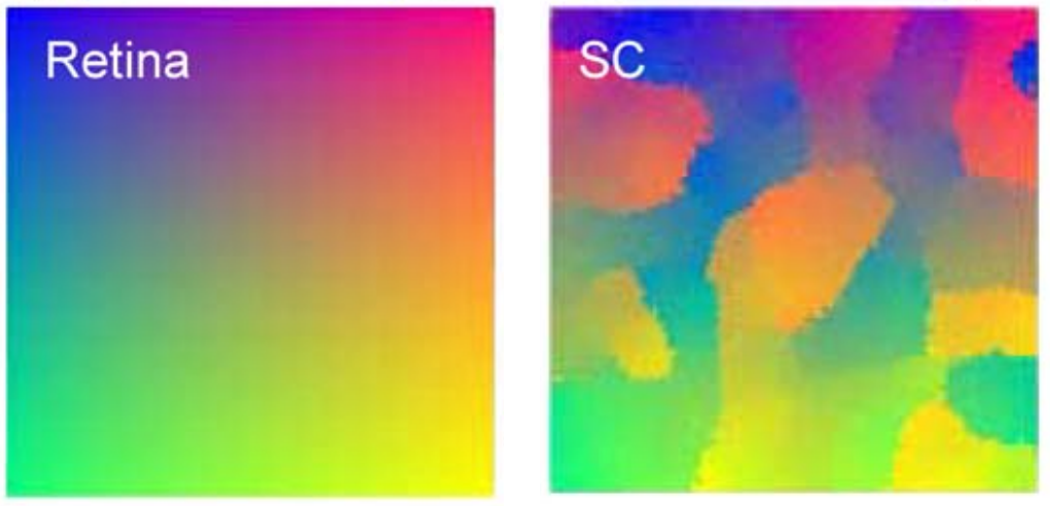
\includegraphics[width = \textwidth]{images/introduction/koulakov_domains}
	\def\c{When the affinity is no longer constrained in a global fashion by chemical guidance cues neuronal activity drives the formation of independent topographic domains. }
	\caption[\c]{\c Each domain is topographic up until its boundary where it permits a discontinuity. These discontinuities imply that the system has not found a global minima, but they also represent local energy minima indicating they are stable. Figure adapted from Tsigankov and Koulakov (2006) \cite{Tsigankov2006-uy}\label{fig:activitydomain}} 
\end{figure}

In the differential formulations these considerations mean that co-activation of retinal neurons $i$ and $j$ result in the synapses defining their arbours moving towards the conjoined centre of mass. This results in a refinement of synaptic arbours to be as geometrically close as possible to synaptic arbours with which their retinal cells receive the most co-activation. The movement is stronger when the retinal origins are also closer to each other: distance-dependent correlation leads to the desired phenomenological effect. This is shown in Figure \ref{fig:activityattraction}.
\begin{figure}[h!]
	\centering
	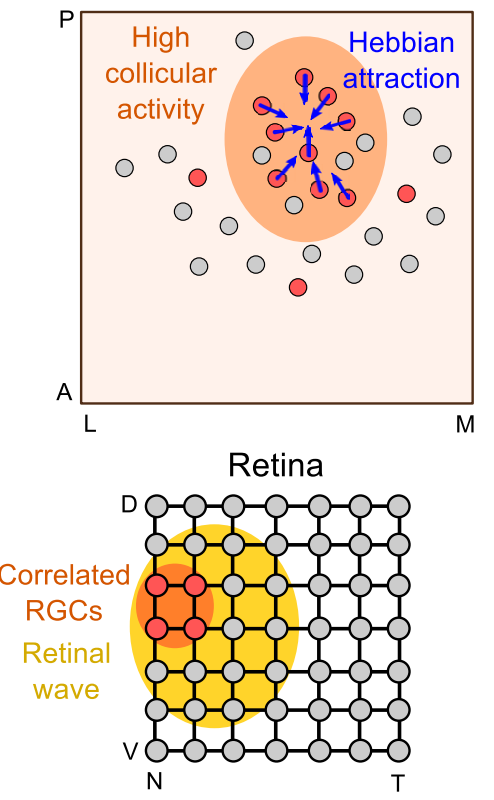
\includegraphics[width = 0.67\textwidth]{images/introduction/cang_attraction}
	\def\c{The effect of co-activation of neurons in the retina is to move their synaptic presence closer to their shared centre of mass. }
	\caption[\c]{\c This effect is most pronounced when retinal cells are frequently co-active. A distance-dependent correlation function then insists on shared topographic domains for neighbouring retinal cells due to a pronounced mutual co-activation of nearby retinal cells. Figure adapted from Grimbert and Cang (2012) \cite{Grimbert2012-cd} \label{fig:activityattraction}} 
\end{figure}


\subsection{Mechanical-sensing Models}
Mechanical sensing is proving to play an important role in the development of the retinotopic projection. Despite this there have been no models dedicated to  explaining and predicting the effects of this mechanism. The role of mechanical sensing with respect to topographic mapping has been most intensively studied in the Xenopus model system and has been used to explain the characteristic turn made by the axonal bundle originating in the retina en route to the tectum \cite{Koser2016-tm}.

\subsection{Unified Models}
More recently the field has converged on unified models involving multiple mechanisms and usually to explain a particular dataset. These models typically apply the general principles outlined above. Four key recent models are detailed which highlight the differences and similarities in the above approaches and demonstrate what steps the field needs to take next.

\subsubsection{Godfrey-Swindale-Eglen}
The Godfrey-Swindale-Eglen (GSE) model is a highly detailed model that aims to be as biophysically accurate as possible with detailed mechanisms included for several known biological processes: axon growth and branching via molecular guidance cues, synapse generation and deletion mediated by trophic factors, a conductance based integrate and fire model of neuronal activity, homeostatic mechanisms for balancing neuronal firing rates, and STDP \cite{Godfrey2009-ts}. There are several potential implications of perturbations to each individual mechanism which will not be elaborated. 
\paragraph{Mechanisms}
The axonal growth model assumes that an axon is composed of a series of individual segments and at each time step there is the possibility of an axon segment growing, or branching. At each segment of each axon there is an affinity associated with a chemotactic cue and a trophic factor and is modelled as a differential equation. The chemotactic affinity for a branch was given by a lock-and-key mechanism which had different functional forms but amount to the same preference for a single location in the target. The different forms mediate the branching process to help the model reproduce the interstitial branching effect \cite{McLaughlin2003-nf, McLaughlin2003-co, Hindges2002-rt}. The growth and branching processes are mediated by an axonal resource which is governed by a differential equation coupled to affinity.

Every five seconds there is a probability of an axon growing or branching which functions of the resources available to the segment and the threshold for each of these. The thresholds are fine tuned arbitrarily, as with the chemo-affinity, to control the phenomenological aspect of branching observed experimentally. Any growth segment with no children also has the possibility of contracting calculated as a function of resources and some unique threshold. The vector along which a growth occurs is a mix of the vector of its parents orientation and the orthogonal vector to the orientation. The relative proportions are controlled so that branching is largely orthogonal with a perpendicular offset  and growth is largely perpendicular with an orthogonal offset. The relative amount of offset is tuned by some parameter. Probabilistically it is relatively clear to see that with a lock-and-key affinity profile and some method by which to maximise this profile each axon will find its correct target. What is novel in this approach is that it allows for the full developmental time-course to be explicitly modelled but requires a high degree of tuning. 

In addition to the growth of an axon the model allows for the generation and deletion of individual synapses. This process is established after the initial growth stage is complete and the neuronal activity mediated through retinal waves stage is initiated. During this stage the axons are still allowed to grow. A standard integrate-and-fire model was employed with a variable conductance mediated by a sigmoid of the ratio between the current firing rate and the target rate to model the post-synaptic firing events. The excitation input to a neuron was modelled as the sum of all incoming synaptic weights scaled to a homeostatic rate function. Pre-synaptic firing events were generated using a Poisson process that was activated when a certain level of recorded calcium activity was exceeded. Synaptic weights were finally scaled according to pre-synaptic and post-synaptic time correlations using an STDP rule. This stage was allowed to continue for 60 hours.
\paragraph{Findings}
The authors examined two major scientific questions: the developmental time course of the map, and the $\beta2^{-/-}$ knock-out. They found that with sufficient tuning the model was able to accurately reproduce several features of the wild-type phenotype notably interstitial branching and a pattern of establishing a coarse topographic map followed by a refinement period. Notably, the model suggests that molecular guidance has a limiting effect on refinement which is a point corroborated by a theoretical analysis from Goodhill \cite{Goodhill2016-ck}. Furthermore, when the activity based refinement period was activated prematurely the authors observed a near complete disruption of the map supporting the notion of a critical period and experimental evidence for the relative timings of guidance and refinement. 

The authors further suggest that a mechanism for synapse creation and deletion mediated by derived trophic factors is sufficient for refinement and that a STDP mechanism contributes little to no effect in the processing of map formation. This prediction was made by completely disabling the STDP mechanism and allowing the map to develop whereby the plasticity is mediated by the number of synapses on a target rather than their strength. However, the reverse experiment was not performed with trophic based synapse creation being restricted and STDP driving synaptic reorganisation. Therefore, the model allows for the possibility of STDP also being sufficient for map formation.

The authors also studied the $\beta2^{-/-}$ knock-out by approximating the data presented by \cite{Stafford2009, McLaughlin2003-nf}. The retinal cells were assumed to be in a bursting state when recorded calcium levels exceeded a threshold allowing the rate of the Poisson process generating spikes in the model to be up-regulated. In this way several activity patterns were examined and the model was able to accurately predict the phenomenology of the $\beta2^{-/-}$ mutant: larger projective and receptive fields. Notably, the authors acknowledge that the quantitative prediction was an order of magnitude different to the observed measurement but this could likely be due to the activity properties of the $\beta2^{-/-}$ not being fully understood. The authors further conjecture that the it is not the particular properties of the waves themselves but the correlation patterns that the waves establish between individual neurons that principally explain the data; see Section \ref{sec:activity}. This is supported by an experiment where activity is entirely decorrelated yielding a lack of retinotopic refinement \cite{McLaughlin2003-yy}.
\paragraph{Key Issues}
The model is able to accurately reproduce several aspects of regular wild-type development in addition to qualitatively reproducing the $\beta2^{-/-}$ knock-out. However no other mutants were described. The lock-and-key mechanism used for chemotaxis means that most chemotactic perturbations will likely be qualitatively accounted for, however examination of the $Math5^{-/-}$ mutant would be of keen interest given the resource not space based competition mechanism.

Each stage of the model has required a degree of parameter tuning completed by the expert. To rigorously establish these parameters scientifically it would be valuable to estimate these tuned parameters statistically with reference to a dataset. However, the computationally demanding runtime makes this prohibitively expensive. The model is therefore most useful as a detailed phenomenological explanatory tool.  A large degree of the runtime arises from the sheer complexity of the model. It involves simultaneous solutions of coupled differential equations corresponding to several mechanisms coupled on thousands of indexes. The authors acknowledge that: ``The complexity of the model made it a practical impossibility to pre-define numerical quantities for the large range of mechanisms represented". Given the number of degrees of freedom it is reasonable to assume that almost any data can be explained with sufficient parameter tuning. While this can offer biological insights it presents a challenge to model interpretability and confidence.

The GSE model while incredibly detailed has several key shortfalls: time, complexity, and to quantitative inaccuracy. The model takes approximately five days to converge which makes exploratory analysis without access to unreasonable amount of computation power impossible. Therefore, the model can, if accurate, only be used for confirmation studies. The computational intensity also limits the models statistical capabilities and makes Bayesian fitting almost impossible. The complexity also allows for a level of fine tuning . Finally, the only phenotype ($\beta2^{-/-}$ mutant) that the model was tested against was quantitatively inaccurate when compared to data.
\subsubsection{Grimbert-Cang}
The Grimbert-Cang model uses two-stage development process which is designed to mimic the development process \textit{in vivo}: retinal afferents are placed in the colliculus stochastically according to their receptor ligand profile using stochastic sampling, then a differential equation formulation of competition and activity is used to evolve the afferents location to their final position. 
\paragraph{Mechanisms}
For the A system stochastic sampling proceeds by defining a probability distribution proportional to a combination of receptors and ligands in both the afferents retinal location and the potential location in the colliculus. This probability is composed as a product of a forward probability (forward signalling) and reverse probability (reverse signalling):
\begin{equation}
P(x_R, x_C) = P_F(x_R, x_C)P_R(x_R, x_C),
\end{equation}
where $P_F$ and $P_R$ are both sigmoid functions of the relative difference in ligand and receptor in the retina and colliculus. Since the two combinations (retinal-receptor to colliculus-ligand, and colliculus-receptor to retinal-ligand) are counter-graded with each other the sigmoid defined by $P_R$ and $P_F$ will have different parity implying a unique location where the probability is maximised. For each axon at $x_R$ a branch location $x_C$ is chosen with uniform sampling and retained with probability $P(x_R, x_C)$. The B system is computed in a simpler fashion each retinal axon is associated with a perfect position $y$ and sampled with an error $E$, then an additional error $e_i$ is added for each branch. This procedure therefore generates a probabilistic arbor for each axon. Since the placement function has unique maximal probabilities this model is a Type II mechanism. Once all branches have been placed the algorithm proceeds with solving the differential equation:
\begin{equation}
\frac{d \vec{x}^C_i}{dt} = \alpha \sum_j W(\vec{x}^R_i - \vec{x}^R_j) F(\vec{x}^C_i - \vec{x}^C_j) - \beta \nabla_CD(\vec{x}^C_i),
\end{equation}
where $\vec{x}^Z_i$ denotes the retinal $Z = R$ and colliculus $Z = C$ locations of the $i$'th axon, $W$ is a function that is assumed to contain all information about the correlation effects of retinal waves and there implicit effect on axonal arborisation, $F$ contains similar information but instead models a ``Hebbian attraction", and $D(\vec{x})$ represents the sum over all axons of a series of Gaussian's centred around the branches locations. The effect of the second term is immediate as in isolation it models the diffusion equation. Thus, it encourages the axonal centres to move down the concentration gradient and with boundary conditions that prevent loss of material will result in the branches being uniformly distributed throughout the target. The first term implicitly adopts the argument laid out in Section \ref{sec:distancecorellation} with a Gaussian correlation in the retina and a non-linear function in the colliculus given by $F(\vec{x}) = K(1-\lVert\vec{x}\rVert_2^2/\theta^2)\vec{x}$ for some $K$, $\theta$ and restricted to the semi-positive domain by mapping all negative values to zero.
\paragraph{Findings}
Using the model the authors examined several phenotypes: WT, the EphrinA triple knock-out, the EphA3 heterozygous and homozygous knock-ins, the EphA7 knock-out, and the p75Ntr knock-out. The model was able to accurately reproduce the phenomenology of each of these phenotypes which in the case of the receptor-ligand perturbations is expected as the model is constructed as a Type II lock-and-key mechanism for chemotaxis. The p75Ntr knock-out involves disrupting a receptor-ligand reaction but is less well understood with experimental results suggesting it is critical for reverse signalling to occur \cite{Lim2008-bq}. The authors found they were able to broadly recreate the phenomenology of the mutant by disabling reverse signalling and tweaking the role of competition which they suggest implicates p75Ntr in retinocollicular competition.
\paragraph{Key Issues}
The authors examined the effect of removing competition on the final maps in some sense in their exploration of the p75Ntr knock-out. They first demonstrate that decreasing the strength competition decreases the total area covered by arbors in the colliculus. It is not clear here if they define the total area to be the union of sets defined by the area function of each retinal axon branch, or conversely the area of the union of all branches. This is a subtle difference with important implications for the $Math5^{-/-}$ mutant. In the second case, provided the map was oriented at the correct boundary, the model would predict the effect of the mutant. However, in the first case it is possible that the retinal afferents spread out uniformly over the entire colliculus but are tightly constrained such that the total arbor areas do not overlap which would not be sufficient to explain the $Math5^{-/-}$ mutant. Given that the chemotactic mechanism is Type II, or lock-and-key, and that the activity mechanism is isotropic it is more likely that the it is the first case, not the second. Therefore, the model is unlikely to reproduce the $Math5^{-/-}$ data.

The model has a two stage representation of time: the initial contacts are placed by random sampling of a distribution in a first stage, and then refined by a differential equation in a second stage. This representation has the advantage of being computationally efficient and reasonably well correlated with known developmental time points. However, as a developmental model it offers little guidance as to how the three mechanisms interact in tandem. Therefore, while it has a differential interpretation of time in the second stage it is not clear that it can be used to make temporal predictions and the model is, for now, best interpreted as an energy minimisation model that uses a stochastic sampler to initialise a gradient descent minimisation scheme. The developmental endpoint, and not the process of minimisation itself, is the scientific relevant component of the model.
\subsubsection{Simpson-Goodhill}
The Simpson-Goodhill model is an updated version of a historical model for topographic development: XBAM \cite{Hope1976-vx, Overton1982-sr}. It uses a differential formulation allowing afferents to move in the space of the superior colliculus on the basis of contributions from three components: fibre-target chemotaxis, fibre-fibre chemotaxis, and competition. Notably, the competitive mechanism acts only on the position of other afferents and is thus a fibre-fibre interaction deviating from the original XBAM which included all fibre-fibre effects in a single term. 
\paragraph{Mechanisms}
The model only considers a given afferent to be associated with a single location in the target and thus the synaptic density function $n$ is a Dirac-Delta allowing functions only of position to be considered in the above formulations. The models iterative procedure is summarised compactly as:
\begin{equation}
\frac{dx_i(t)}{dt} = m_1 \vec{G}_i + m_2 \vec{C}_i + m_3 \vec{I}_i, \label{eq:simpsongoodhilliteration}
\end{equation}
where $\vec{G}$, $\vec{C}$, and $\vec{I}_i$ represents the fibre-target chemotaxis, competition, and fibre-fibre chemotaxis respectively and $m_1, m_2, m3$ are scaling constants. The index $i$ represents an afferent which represent branches of RGCs and therefore multiple values of $i$ can contain the same receptor and ligand information. The fibre chemotaxis is implicitly defined with each branch being associated with an optimal location in the colliculus for which it has highest affinity. This corresponds to an implicit Type II mechanism and allows the problem to be explored in a general sense but makes it difficult to explore development with data driven phenotypes without first knowing the phenotypic effect. Letting $\vec{x}_{i_0}$ be the location with highest affinity for branch $i$ be the chemotaxis movement vector is given by:
\begin{equation}
\vec{G}_i = \vec{x}_{i_0} - \vec{x}_i.
\end{equation}
The competitive term is represented in a similar way to the ``Hebbian attraction" term in the Grimbert-Cang model, but with different sign. Each branch is assumed to have an interaction radius $r$ in which it can be repelled by other branches. The weight of repulsion between two tips is given by $W(i, k) = (1 - \lVert \vec{x}_i - \vec{x}_k \rVert_2/2)$ and the total repulsive action provided by a set of $N$ branches $B_i$ within radius $r$ with a branch $i$ is given by:
\begin{equation}
\vec{C}_i = \frac{1}{N} \sum_{k \in B_i} W(i, k) \frac{(\vec{x}_k - \vec{x}_i)}{\lVert \vec{x}_i - \vec{x}_k \rVert_2}.
\end{equation}
The fibre-fibre interactions are modelled by introducing the idea of a discrimination limit first proposed by Reber et. al. (2004) \cite{Reber2004-wq}. The mechanism is summarised by the notion that two incoming afferents can sense their relative receptor levels but below some limit cannot discriminate whether they have the same retinal origin. If they can discriminate then they apply a repulsive force on each other which is modelled in the same fashion as competition. The level of retinal receptor for branch $i$ used to make the discrimination decision was based on reported mRNA measurements and is given as $R_i(x_{r}) = 0.26\exp(2.3x_{r}) + 1.05$ where $x$ represents the canonical projection from $\vec{x}$ to the retinal location along the NT axis. The function used to make the discrimination was $Q(R_i, R_k) = R_i / R_k$. Note that this discrimination function corresponds to forward signalling under the seminal Geirer model \cite{Gierer1983-tn}. The fibre-fibre movements are given by:
\begin{equation}
\vec{I}_i = \frac{1}{N} \sum_{k \in B_i} W(i, k) \frac{(\vec{x}_k - \vec{x}_i)}{\lVert \vec{x}_i - \vec{x}_k \rVert_2} \quad Q(R_i, R_k) > s.
\end{equation}
The model is initialised by placing all branches along the rostral border of the colliculus and the differential equations are solved for each branch until a stable fixed point is reached. 
\paragraph{Findings}
The authors then used the model to phenomenologically reproduce several examples in three classes of experiments: surgical intervention, gradient perturbation, and branch number suppression. The surgical intervention studies involve reproducing a series of experiments involving graft rotation, graft translocation, retinal and tectal ablations, initialisation mismatches, and compound eyes. The essential finding was that even with a constraining competitive mechanism the chemotactic cues were able to guide a reformation of the maps to match experimental data. The authors note that these experiments have been difficult to reproduce in some models, and have not been attempted by others \cite{Goodhill2005-ly, Purves2001-lr}. The gradient perturbation studies focused on the EphA3 knock-in phenotypes and is able to successfully reproduce the collapse phenomena and by varying the interaction of the three terms they conclude that all three mechanisms of chemotaxis, fibre-fibre interactions, and competition are necessary.  

\paragraph{Key Issues}
The principle issues with the model are with the choice of chemotaxis mechanism and the lack of activity. The chemotaxis mechanism is defined implicitly which allows for a near perfect specification of programmed target destinations and a key criticism here is that absolute knowledge about a targets destination weakens the strength of the studies reproducing gradient perturbations - the EphA3 phenotype is simulated by inverting its functional form to find appropriate targets which can be seen as putting the cart before the horse when aiming to replicate the effect of the perturbation. The model also has no mechanism for modelling the effect of activity which makes it difficult to assess various activity based perturbations.
\subsubsection{Tsigankov-Koulakov \label{sec:koulakov}}
The Tsigankov-Koulakov model has gone through several iterations being built up piecemeal \cite{Koulakov2004-ia, Tsigankov2006-uy, Tsigankov2010-on, Triplett2011-jk, Wei2013-jw}; attention is focused on the 2011 iteration which has been used subsequently to explore several biological and theoretical questions \cite{Triplett2011-jk, Savier2017-wt, Tikidji-Hamburyan2016-sn}. 
\paragraph{Mechanisms}
In essence the model postulates that each potential map can be represented by a discrete function mapping the colliculus to the retina and the biologically appropriate map minimises an energy functional which is composed of three elements corresponding to chemotaxis, activity based refinement, and competitive interaction.
\begin{align}
&E = E_{\text{chem}} + E_{\text{act}}+E_{\text{comp}}\\	
&E_{\text{chem}} = \sum_{p \in \{\alpha,\beta\}}\sum_{i \in \text{syn}} pR(i_\text{ret},p)L(i_\text{col},p) \\
&E_{\text{act}} =- \frac{\gamma}{2} \sum_{i \in \text{syn}}\sum_{j \in \text{syn}} C(d_R(i, j))U(d_C(i, j))\\
&E_{\text{comp}} = \sum_{i\in \text{ret}} (n_i^2 - 500 n_i^{1/2}) + \sum_{i\in \text{col}} n_i^2.
\end{align}
The chemotactic term is given with $\alpha90$, $\beta=-120$ with the change in sign indicating that the B system is attractive and the A system repulsive, $R$ and $L$ are the masked gradients (the difference between Eph and ephrin levels) in retina and SC locations respectively, and the sum is performed over all possible synapses; the parameters and gradients are inherited from previous iterations of the model. It is important to note that this masking ensures that the system is a Type I or graded matching. The activity term is the sum over all pairs of synapses of the product of two correlation functions which take the normed distance between a synapse pair in the retina, $C(d_R) = \exp(-|d_R|/11)$, and colliculus, $U(d_C) = \exp(-d_C^2/18)$, where the $d_R$ and $d_C$ are the metric functions for the retina and colliculus respectively and the parameters $11$ and $18$ and $\gamma=0.05$ are inherited from previous iterations; the forms are claimed to fit biological measurements of correlation of activity but so far only measurements of spontaneous retinal activity have been made \cite{Stafford2009}, and it is unclear precisely how to define correlation \cite{Cutts2014-mn}. Finally, the competition term is given by two sums: one over over the SC and retinal locations. The sums compute the square of the number of synapses for the SC sites, and the difference between square and square root of the number of synapses for the retinal sites. In this fashion, it is energetically favourable to have some, but not too many synapses between locations. The forms and parameters of the function are chosen arbitrarily.

The minimisation procedure for the model is similar to that of a Metropolis-Hastings model \cite{Gelman1995-uj}. At each simulation point a potential pairing of an SC and retinal site is considered and the change to the energy function that adding this site would induce is calculated. A uniform random number $u$ is generated and compared to:
\begin{equation}
p = \frac{1}{1+\exp(-4\Delta E)},
\end{equation}
and the change is accepted if $p<u$ thus promoting changes which lower the energy whilst stochastically accepting higher energies infrequently. The same procedure is repeated except sampling amongst existing synapses and preferentially deleting synapses which contribute high energy. It is claimed that this procedure converges to a minimum within $~10^7$ simulation steps with map standard deviation changing only $0.5\%$ over the order of magnitude $10^6-10^7$ change \cite{Tsigankov2006-uy}. However, it cannot formally converge to an energy minimum - it can only potentially converge to a stationary distribution of synapses as that is what is being sampled, not the energy.
\paragraph{Findings}
The model has been broadly successful in various aspects of retinotopic development. This has been, in part, due to an active development and refinement of the model structure and components by a large number of participants in the field. The first unified version of the model reproduced the ephrinA2 and ephrin-A2A5 knock-out phenotypes \cite{Tsigankov2006-uy}. This version of the model was later used to analyse an important dataset containing EphA3 heterozygote, homozygote, and a cross-breed of the EphA3 heterozygote with the $\beta2^{-/-}$ mutant.

The current version of the model was designed to account for the $Math5^{-/-}$ mutant by reworking the competitive mechanism implicitly defined in the original unified model \cite{Triplett2011-jk, Tsigankov2006-uy}. This finding was reproduced in later analysis which found the model could partially reproduce the ephrin-A2A3A5 triple knock-out data by generating patches, but no global order, and accounted for EphA3 heterozygous and homozygous phenotypes \cite{Hjorth2015-le}. The model has also been used to explain broader aspects of the visual system such as alignment mechanisms between the SC and V1  \cite{Savier2017-wt}. Interestingly, when attention was turned to studying $\beta2^{-/-}$ mutants the model has had mixed success. It has first been studied in the context of an EphA3 homozygous knock-in and $\beta2^{-/-}$ mutant by \cite{Tikidji-Hamburyan2016-sn} which replicates the data presented by \cite{Triplett2012-ap}; coincidentally it is one of the few studies to conduct a parameter sensitivity analysis using a week of supercomputing time and highlighting the difficulty of such a study. Another line of study found that manipulation of the activity components was insufficient to explain $\beta2^{-/-}$ mutant data requiring the chemotactic parameters to be tuned to match development time courses \cite{Lyngholm2019-fs}. 
\paragraph{Key Issues}
There are a number of open theoretical and biological questions relating to this model. Principally, does the minimisation procedure have a biologically meaningful interpretation? Some studies use only a sample from the stationary distribution as the representation of the map; other work has claimed that the switching procedure itself can give insight to the developmental processes driving map formation \cite{Lyngholm2019-fs}.

Currently, it is difficult to formally translate the model to biological data and vice-versa; it is relatively easy to manipulate gradients and activity functions and generate phenotype data but there are no examples of how to statistically quantify the model goodness of fit and most claims are thus made qualitatively. It would be valuable to understand the sensitivity and robustness of parameter choices in the model as currently the parameters are chosen arbitrarily or inherited from previous work under the assumption that the new model will behave stably. Interestingly, two studies have been performed in this regard and both highlight the challenge of the undertaking \cite{Tikidji-Hamburyan2016-sn}.
\subsection{Comments}
There are few general comments that can be made about retinotopic models at this point. The notion of universal functions, the differences between energy minimisation and differential formalisms, and model assessment with regards to data will be discussed.
\paragraph{Chemotaxis}
Graded matching is to be the only mechanism likely to reproduce the $Math5^{-/-}$ mutant. The lock-and-key mechanism is too prescriptive in most cases to allow for modifications made by radially symmetric mechanisms such as competition to be meaningful outside of corrective procedures. Graded matching allows for the boundary asymmetry necessary in the $Math5^{-/-}$ mutant. This is not to say that counter-gradient mechanisms are not essential but they must be necessarily imbalanced requiring them to work in tandem with additional mechanisms; this idea of competition working alongside bidirectional signalling was explored by Sterratt (2013) \cite{Sterratt2013-ev}. This also partially explains why the Tsigankov-Koulakov model was the only unified model which attempted to explain the $Math5^{-/-}$ mutant, although this was by design, and why the updated Geirer model was able to account for it when explored by Hjorth et al (2015) \cite{Hjorth2015-le}.
\paragraph{Time \label{model:time}}
An important exploratory feature of a model is to predict how a system will evolve over time. Given how difficult it is to acquire data in developing biological systems due to their definitionally changing nature such as growth, or constraints of experimental methodology e.g. an injection experiment that needs to sacrifice the animal thus terminating the development. Most models have been designed and tuned for development endpoints, and particularly in the case of affinity based formulations have no immediate notion of time as in the Tsigankov-Koulakov model. An attempt to explain time sensitive development data with the Koulakov model was made by associating iterations of the algorithm with time steps but it was found that small changes to developmental mechanisms such as activity had the opposite effect predicted by the data and other regulatory mechanisms had to be tuned to compensate \cite{Lyngholm2019-fs}. Differential based formulations such as do have a natural interpretation of time and thereby offer a way to compare and falsify models against experimental data as well as generating time-dependent hypotheses. Most energy based models can be minimized with a differential evolution scheme and the next class of models should exploit this feature to naturally embed time.
\subsection{Model Assessment \label{model:assessment}}
A major hurdle that any modelling work must clear is demonstrating explanatory power of data. This is most frequently done in biological sciences by the use of statistical tests which either allow discrimination and ruling out of certain hypotheses by hypothesis testing, or demonstrating goodness-of-fit under some measure such as a correlation coefficient. Models may also be examined qualitatively, or quantitatively under more bespoke or tailored measures to demonstrate they can accurately reproduce the data phenomenologically; the assumption is that if the model can accurately reproduce the phenomenon then the mechanisms of the model can be analysed to infer how the mechanisms might work in the system of interest. It is the second approach which has garnered the most success in modelling mouse retinotopy. While this approach has been successfully in the generation of scientific hypotheses it has several drawbacks. Its predictive power is limited because a phenomenological model is not intended make explicitly measurable predictions testable by statistics.

A review of existing retinotopic models was taken to assess which model offered the most parsimonious explanation of the data. It was performed using a combination of parameter fixing-to-fit and quantitative analysis using the Lattice Method which allows for a topological rather than registered assessment of the model output. It was found that the most recent Tsigankov-Koulakov model offered the best explanation. To date this model lacks a statistical understanding of its parameter space with parameters most often being chosen \textit{ad-hoc} to support the argument at hand. This is notable because the parameter space of this model is large, $>11$ parameters, and it can feasibly generate functions universally and therefore without rigid constraints on its parameters its explanatory power is significantly weakened. 

The reason for the lack of parameter analysis in retinotopic models more generally is because it has significant technical challenges. Focusing on the Tsigankov-Koulakov model again observe that it has computational complexity of at least $O(n^6)$ but more likely on the order of $O(n^8)$ in the number of retinal cells, $n$. A parameter space grid search was performed as part of a Masters thesis which demonstrated this challenge restricting its search to a coarse grid on low resolution (I. Stark, personal communication, July 12, 2018). This computational cost makes even embarrassingly-parallel approaches to large-scale statistical searches prohibitively high.

A recent data-set that allows for the challenge of statistical hypothesis testing and formalised model hypotheses was published by Owens et al. (2015) \cite{Owens2015-zv}. This data-set presents a challenging hypothesis to current understanding of retinotopic mapping suggesting a high degree of stochastic behaviour in the EphA3 mutants. However, the methods of assessment do not attempt to analyse this randomness by summary statistics in their modelling account and so the question remains open. 
\section{The Elastic Net and NP-Complete Problems \label{sec:heuristics}}
An NP-complete problem is one which is not known to have a deterministic polynomial time solution, can have an easily verifiable solution generated by brute-force, and is reducible to other NP-complete problems in polynomial time \cite{Garey1990-th}. The Travelling Salesman Problem (TSP) is perhaps the most well known of these and has a super-polynomial complexity bound: $O(n^2 2^n)$. The TSP is stated quite simply: given a collection of nodes with a notion of paths between them with some defined distance find the shortest path that visits all nodes exactly once returning to the point of origin \cite{Applegate2007-nz}. 

\begin{figure}
	\begin{subfigure}{0.5\linewidth}
		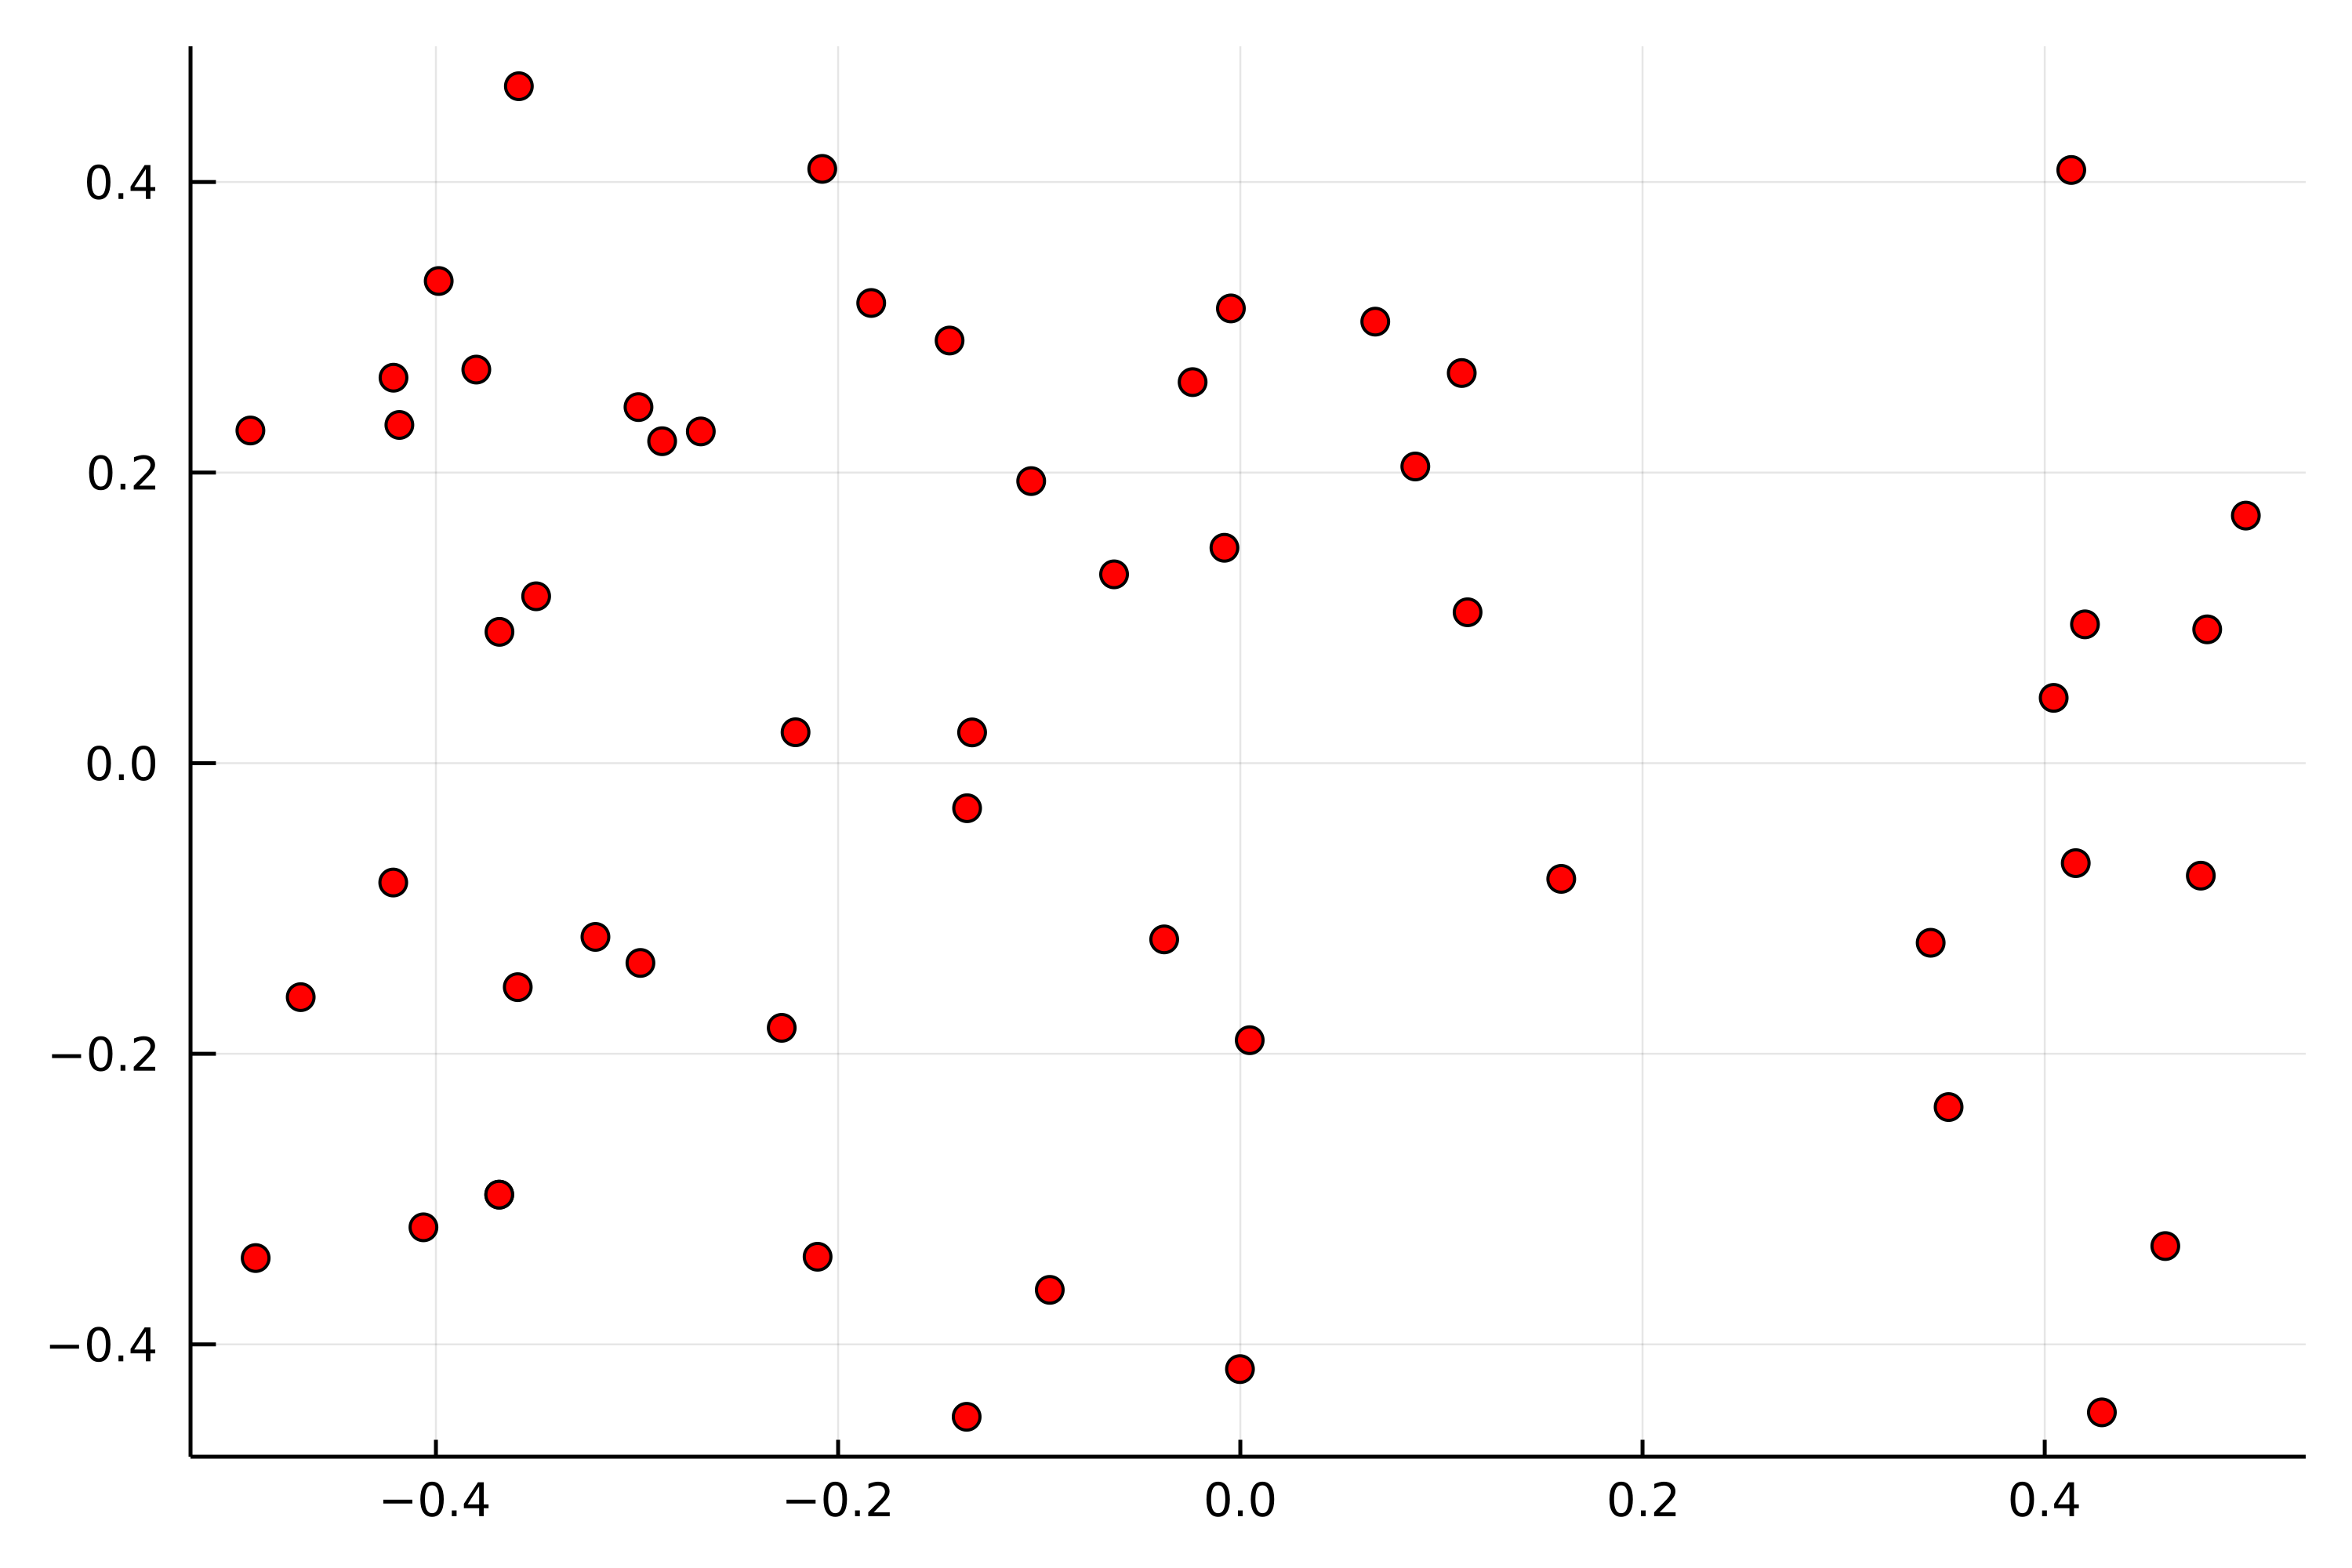
\includegraphics[width = \textwidth]{images/introduction/tourscatter}
		\caption{} 
	\end{subfigure}
	~
	\begin{subfigure}{0.5\linewidth}
		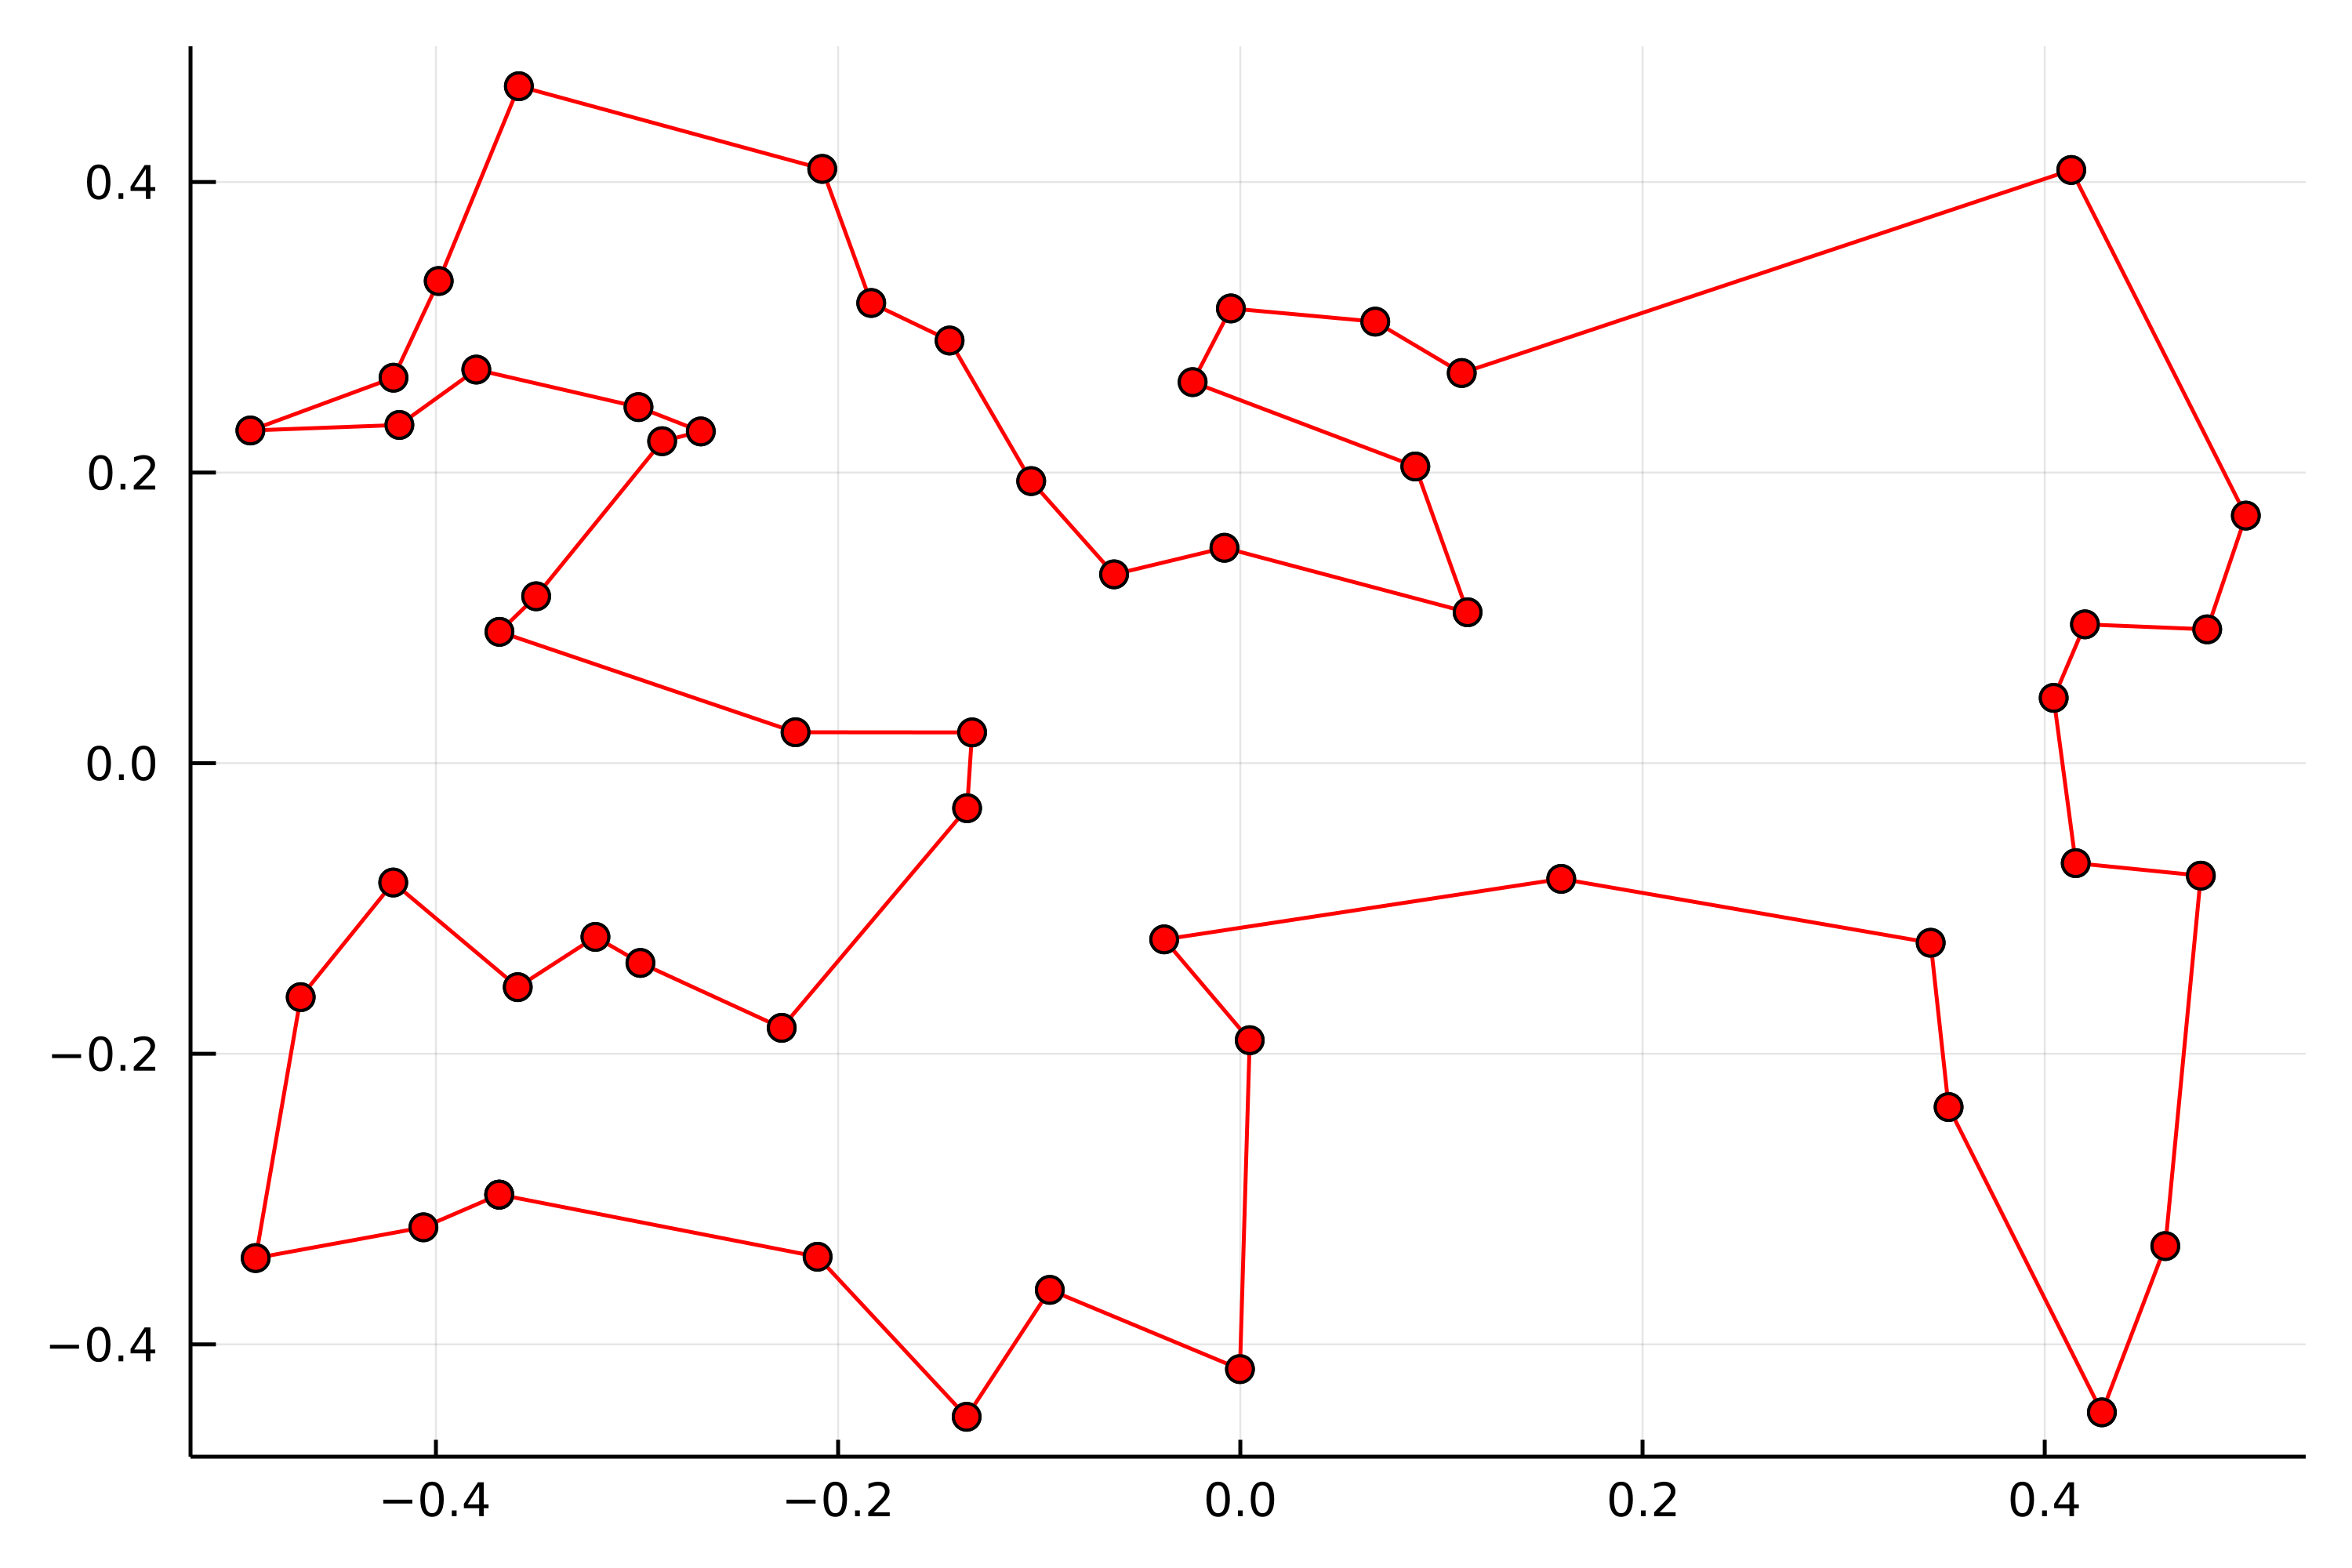
\includegraphics[width = \textwidth]{images/introduction/tourvalid}
		\caption{} 
	\end{subfigure}
	\def\c{A description of the Travelling Salesman Problem. }
	\caption[\c]{A series of nodes scattered uniformly in the unit square is shown in the left panel (a) while a valid tour passing through each of these nodes once before returning to the initial node is shown in the right panel (b). There are n! such tours and while this example does not exhibit a tour crossing they are ostensibly possible. Due to the metric triangle inequality any tour with a crossing can be improved and they are thus provably sub-optimal.}
\end{figure}

There is an interesting relationship with the TSP and topographic maps which was first introduced by the Elastic Net algorithm a heuristic designed to solve the metric Travelling Salesman which was a successor to the Tea-Trade model of retinotopic development \cite{Durbin1987-ki, Willshaw1976-ew}. The model is an energy minimisation model which deforms a net of elastic beads, where neighbours are connected elastically by spring forces, to a set of nodes which provide attractive forces to each of the beads. Supposing that there are $N$ nodes and $M$ beads and letting $X = \{\vec{x}_i : i = 1, ..., N \}$ and $Y = \{\vec{y}_i : i = 1, ..., M \}$ the energy of a given bead configuration is given by a functional parametrised by $\alpha, \beta, K$:
\begin{equation}
E[Y|X; \alpha, \beta, K] = -\alpha \sum_{i = 1}^{M} \log \left( \sum_{j=1}^N \exp\left ( \frac{- \lVert \vec{x}_i - \vec{y}_j \rVert^2 }{ 2 K^2 }  \right) \right) + \beta \sum_{j=1}^{N} \lVert \vec{y}_j - \vec{y}_{j-1} \rVert^2,
\end{equation}
In the limiting case of $K\rightarrow0$ the attractive energy provided in the first term is only significant in a small radius around each node while the tension term dominates in all other areas. The local minima of this functional in this limit are therefore straight line geodesics corresponding to the tension term that travel between each of the cities. Thus, these minima correspond to valid tours of the TSP. The functional can be minimised by gradient descent to find a local minima $K$; see Section \ref{sec:minimisation}. The gradient is calculated as:
\begin{equation}
\partial_t \vec{y}_j(t) = \beta K \left(\vec{y}_{j-1} - 2 \vec{y}_j + \vec{y}_{j+1}  \right) + \alpha \sum_{i = 1}^M (\vec{x}_i - \vec{y}_j) W(\vec{x}_i, \vec{y}_j, K(t); Y),
\end{equation}
where $W(\vec{z}_i, \vec{y}_i, K; Y) = \exp(- \lVert \vec{x}_i - \vec{y}_j \rVert^2 / (2 K^2)) / \sum_{j = 1}^N \exp(- \lVert \vec{z}_i - \vec{y}_j \rVert^2 / (2 K^2))$. This rule is applied 25 times for each $K$ after which $K$ is reduced by the mapping $K\leftarrow0.99K$. When $K$ has reached a sufficiently low value the procedure is terminated. A cartoon of this procedure can be seen in Figure \ref{fig:encartoon}.

\begin{figure}
	\centering
	\includegraphics[width=\textwidth]{images/introduction/elasticNetexample}
	\def\c{A description of the Elastic Net method for producing solutions to the Travelling Salesman Problem. }
	\caption[\c]{\label{fig:encartoon} The Elastic Net is initialised in a circle of radius 0.2 around the centre of mass of the nodes. As K is decreased exponentially and the algorithm moves through its gradient descent the beads are deformed (a-d). K must decrease sufficiently slowly to prevent edge cross-overs; an almost cross-over is shown in (c). This cross-over prevention significantly hampers algorithmic performance as there is no native penalty imposed on cross-overs. The reason decreasing K slowly ensures crossover prevention is due to a sufficiently slow descent being homotopic and thus topologically preserving winding number which must be the same as the initial circle for a tour without crosses. The final tour found by traversing the configuration in (d) is shown in (e) while the best known tour is shown in (f).  Figure adapted from Durbin and Willshaw (1987) \cite{Durbin1987-ki}}
\end{figure}

Development of the Elastic Net has focused primarily on parameter selection with analysis determining optimal rules of thumb for setting the $\alpha/\beta$ ratio and discussion about the limiting aspects of this and how they may be compensated with additional parameter manipulation such as the node-bead ratio \cite{Simmen1991-hm, Durbin1989-gs}. A variation of the Elastic Net was proposed to give substantial computational performance reducing the amount of information considered at each step with minimal performance loss \cite{Boeres1992-fo, Burr1988-fg}. As a TSP heuristic the Elastic Net has been largely superseded with the two predominant heuristics being the Lin-Kernighan heuristic (LKH) developed by Helsgaun, and an Edge-Assembly-Crossover Genetic Algorithm (EAX-GA) being the most successful and of primary interest to this work \cite{Honda2013-ri, Nagata2013-we, Lin1973-pt, Helsgaun2009-dl}. There have been many other biologically inspired heuristics with varying degrees of performance but these will not be detailed further.  

Remarkably, the Elastic Net model was then generalised and reverse engineered to generate topological feature maps: maps whereby a visual feature such as orientation selectivity is smoothly varied across the cortical sheet \cite{Bednar2016-lg}. The generalisation was made by allowing interactions between all beads in the net, not just indexed neighbours. This is an example of a bead stencil and general theory of these stencils is given by Carreira-Perpinan and Goodhill (2011) \cite{Carreira-Perpinan2011-aa}. An account of these phenomena were given by Mitchison and Durbin (1989) who argued that these could be understood in the context of the Elastic Net performing a dimension reduction onto the 2D cortical sheet. This reduction preserves continuity and critically maintains a low wiring cost suggesting that the brain evolved minimal wiring principles and the Elastic Net was one such minimisation scheme \cite{Durbin1990-tn}. The minimal wiring principle has received much attention as a guiding organisational principle \cite{Chklovskii2004-da}. The Elastic Net model was able to generate and account for orientation selectivity, retinotopy, and ocular dominance \cite{Goodhill2000-on, Goodhill1994-dn, Goodhill2000-vp, Goodhill1990-dr}. Interestingly, the introduction of the orientation variables resulted in a deformation of normal retinotopy with the map being highly concentrated around regions of rapid change in the orientation variable; see Figure. This stood as a prediction of the model but optical imaging generated maps of V1, which encodes orientation selectivity, in mice do not appear to show this distorted retinotopic representation in either bulk or phase based measurements; see Figure \ref{fig:v1retinotopy}. 
\begin{figure}
	\centering
	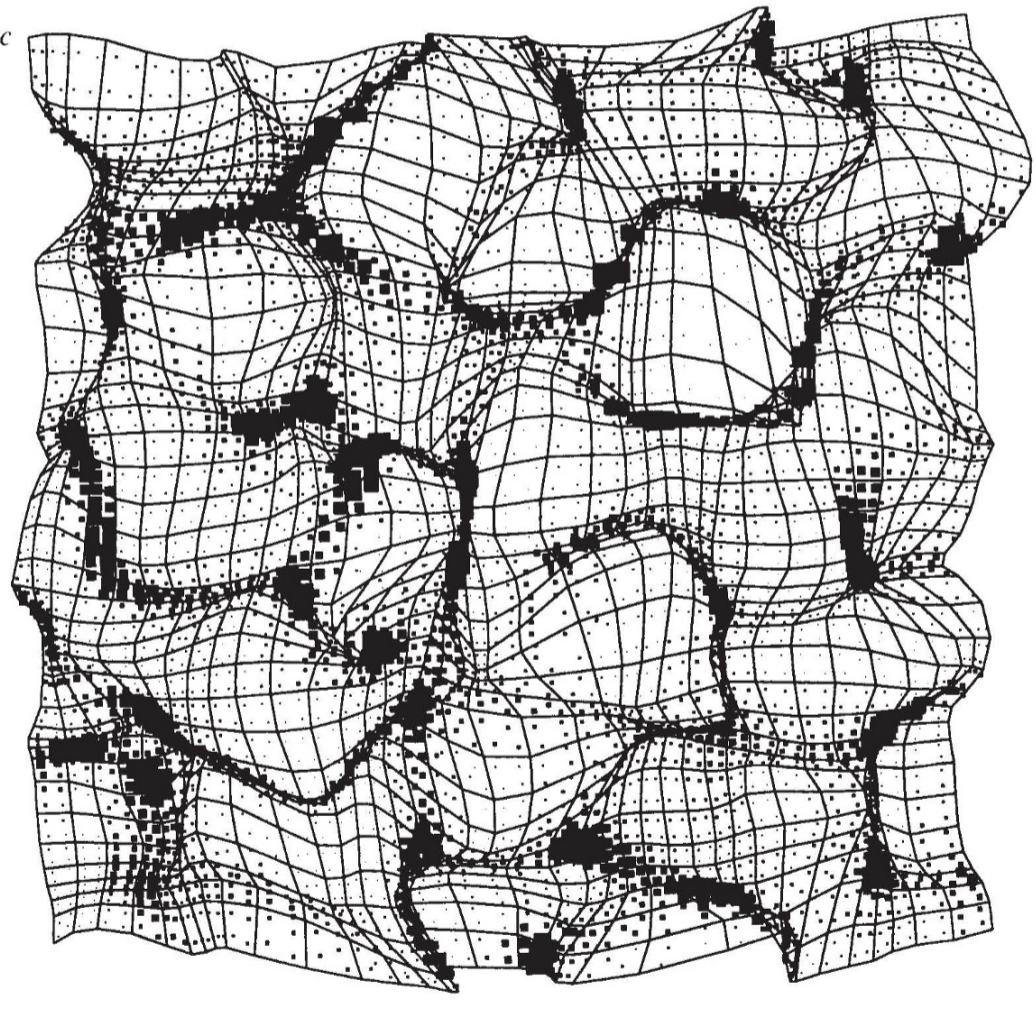
\includegraphics[width=\textwidth]{images/introduction/distortedretinotopy}
	\def\c{Prediction of retinotopy generated by the Elastic Net model when orientation curves are simultaneously trained. }
	\caption[\c]{\label{fig:distortedretinotopy} \c Trained retinotopic locations are given by the intersection of the grid and the size of the black squares indicates the rate of change of the orientation variable. Distorted retinotopic fields are generated around regions where the orientation selectivity changes most rapidly. Figure adapted from Durbin and Mitchinson (1990) \cite{Durbin1990-tn}}
\end{figure}


\begin{figure}
\centering
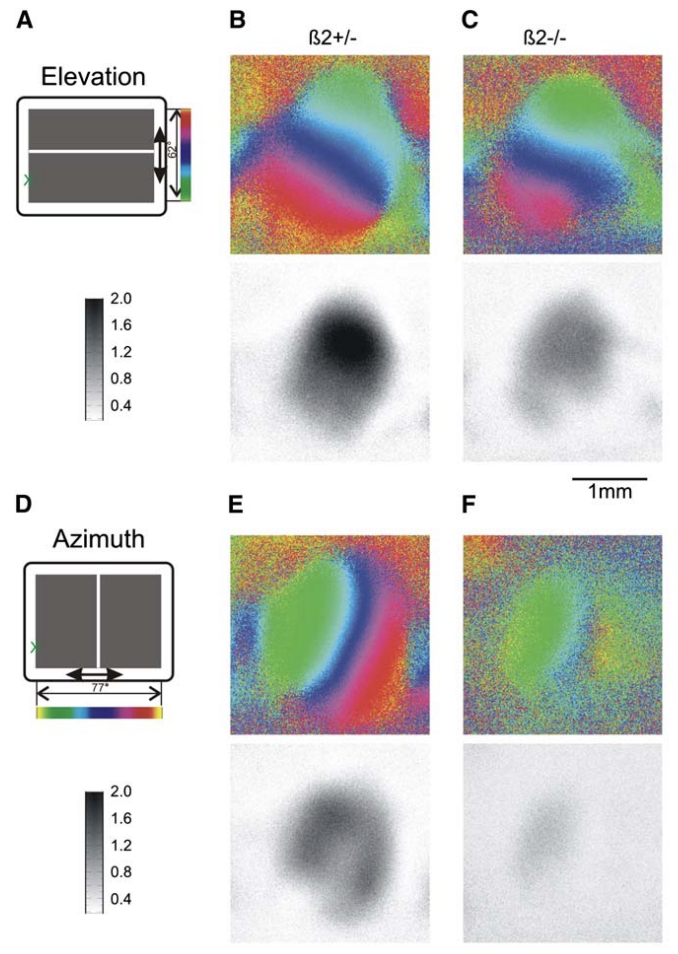
\includegraphics[width=\textwidth]{images/introduction/V1retinotopy}
\def\c{Observations of the uniformity of topographic maps formed in the retinotopic map in mice. }
\caption[\c]{\label{fig:v1retinotopy} Optical imaging scans in both azimuthal and elevational of two phenotypes of regular (B) and deficient (C) spontaneous activity patterns. In both instances the phase and bulk activity scans do not show a distorted retinotopic map. Figure adapted from Cang et. al (2005) \cite{Cang2005-eg}}
\end{figure}
\newpage
\section{Conclusions and Existing Problems}
The field of retinotopic map development has matured to the point of having relatively well understood development mechanisms and frameworks in which to embed them. There is a clear need to understand the effects of activity and in particular predict the organisational properties of the $\beta2^{-/-}$ mutant development. Key issues for the current class of unified models are parameter sensitivity and statistical analysis, and a method to link time courses in the model with developmental time courses present in biology. The understanding of development mechanisms guiding map development have matured and could be incorporated into a heuristic optimiser to aid in solving NP hard problems efficiently.
\subsection{$\beta2^{-/-}$ mutant Analysis \label{sec:beta2justification}}
The majority of recent modelling work has focused on explaining phenotypes of genetic manipulations of gradients with a particular focus on the EphA3 knock-in \cite{Savier2020-xb}. The $Math5^{-/-}$ mutant has garnered some attention but is limited due to the sparsity of available data and the modelling results only serving to confirm existing theory \cite{Triplett2011-jk, Hjorth2015-le}. An active area of experimental research is the $\beta2^{-/-}$ mutant mouse phenotype  \cite{Stafford2009, Dhande2011-jp, Chandrasekaran2005-ug, Xu2015-uc}. Despite this activity only three models have been proposed to explain the principle result: the wider arborisation of the retinal afferents. Of these three models two will be discussed because while the third claims to reproduce the phenotypic effects it offers no detail on the model construction or implementation which prohibits any meaningful interpretation \cite{Xu2011-mt}.

The GSE model uses a wider correlation function alongside an integrate-and-fire spiking model coupled with STDP to model the phenotype and found that while a wider arborisation could be predicted it was an order of magnitude larger than experimental results. It should be noted that the GSE model introduced the activity mechanism after a period of chemotactic development. When the mechanism was introduced earlier it disrupted the development of all topography. It should be noted that the GSE model is extremely computationally demanding taking on the order of five days to generate a single map. It is therefore infeasible to come to a reliable understanding of the variance in its generative mechanisms when tuning parameters to experimental data. The GSE study concluded that it was unlikely that the spatio-temporal statistics of the retinal waves played any role in the developmental process.

The second model attempted to modify the correlation functions in the Tsigankov-Koulakov formalism according to experimental data. The result was reproducing features of the wild-type maps that the model typically generates, but at a much faster rate. Since this formalism instantiates activity purely on distance-based correlations this result suggests that the spatio-temporal structure of the waves may be important, contradicting the conclusion of the previous study.

The body of experimental work suggest a keen interest in understanding the $\beta2^{-/-}$ mutant phenotype but the currently proposed models have had limited success in predicting the primary experimental result. The seeming contradiction in conclusions about the effect of spatio-temporal statistics in existing models suggest that a more detailed theoretical understanding of this aspect of the phenomenon is required. Furthermore, a model must be sufficiently lightweight in both parameter space and execution time to offer meaningful statistical comparison to available data. The development and analysis of this model will be the focus of Chapter \ref{chapter:neuralstdp}
\subsection{EphA3 Knock-In Dataset }
The dataset by Owens et al (2015) presents some interesting challenges principally in the argument or interpretation of the data. Under their interpretation the EphA3$^{+/-}$ map is driven by a stochastic process resulting in the single knock-in maps presenting occasionally as single, mixed, or double maps \cite{Owens2015-zv}. Additionally, $\beta2^{-/-}$ mutants were crossed with EphA3 knock-ins and examined. The paper suggested that these mutants presented a wild-type phenotype with slightly lower amplitudes. They thus proposed a competitive balance of molecular and activity based cues which results in map heterogeneity. 

The stochastic component of the argument is further justified by the use of an early version of the Koulakov model which the authors claim to reproduce the stochastic behaviour observed in the data. Furthermore, in this version of the Tsigankov-Koulakov model competition is implicitly defined by the requirement of a one-to-one mapping which leads naturally to interdigitating maps when chemical affinities are identical. This strict competition mechanism could thus produce maps which appear stochastic arising from the minimisation procedure, but do not represent biologically plausible maps i.e. this effect may be an artefact of the modelling. Interestingly, a modelling study using the updated version of the Tsiganov-Koulakov model were able to reproduce the $\beta2^{-/-}$EphA3$^{+/+}$, and EphA3$^{+/+}$ phenotypes lending some support to the original hypothesis. An analogous study modelling $\beta2^{-/-}$ effects in a similar way concluded that this method meant the activity effects had become dominant in the model \cite{Lyngholm2019-fs}. Activity is sufficient for unoriented topography and a model of neural activity has shown to be able to correct defects in poorly established topographic mappings with a secondary study showing the model can account for the widened arbors in the $\beta2^{-/-}$ mutant \cite{Chandrasekaran2005-ug, McLaughlin2003-yy}. Taken together, these results imply that the choice of modelling parameters resulted in a strong activity dominating any map aberrations introduced by the modified EphA3$^{+/-}$ gradient and producing the desired phenotype, but in the absence of EphA3$^{+/-}$ modelling does not imply stochastic balancing behaviour.

Preliminary unpublished analysis by David Willshaw revealed that the prevalence of stochastic seeming phenotypes might have stemmed from a miscategorised data point: a homozygote was labelled as a heterozygote. Taken in conjunction with analysis restricted to one dimension and a confounding factor in the modelling suggest that the data should be re-evaluated. To understand this dataset more thoroughly two things are essential: a revisiting of the map data analysis including all available 2D data about the map and a robust analysis method, and a modelling study of the EphA3+/- single knock-in using the updated Tsigankov-Koulakov model. Further to this, a reanalysis presents an excellent opportunity to understand the statistical properties of the Tsigankov-Koulakov model. Analysis on this dataset will be performed alongside theoretical analysis in Chapter \ref{chapter:lattice}.
\subsection{Efficient Unified Modelling \label{sec:efficientmodelling}}
A key issue of recent unified models of topographic map formation is a lack of understanding in the model parameter space and how these parameters change when considering different mutant data. The near universality of many models ensure that with sufficient parameter tweaking a desired outcome can be achieved which makes model assessment challenging. A proposed pipeline for model assessment was given by Hjorth et. al. (2015) but the problem of understanding how the parameters can be manipulated remains. These studies are limited principally because the models are computationally demanding. The only known parameter sensitivity study on the Tsigankov-Koulakov formulation required typically unobtainable amounts of super computer time \cite{Tikidji-Hamburyan2016-sn}. These make parameter fitting methods and various statistical methodologies out of reach.

Therefore, there is a pressing need to reformulate the salient features of the unified models into a computationally efficient format that does not comprise explanatory power. The most parsimonious explanations of modelling data are given by the Tsigankov-Koulakov model and therefore it seems reasonable to exploit the principle features of that model: graded matching, distance dependent correlation functions, and competition based on some polynomial function of synaptic density. The model however does not have a natural interpretation of time and relying on a stochastic minimisation procedure. The Simpson-Goodhill and GSE models fare well in this regard as their differential formulation allow a natural way to correlate the development of the model with developmental time points in the system. Fortunately, there is a natural way to reformulate energy based functional models into differential ones through the gradient descent method of functional minimisation; see Section \ref{sec:graddescent}. The development of this computationally efficient formulation shall be the subject of Chapter 4.

\subsection{Heuristics}
The Elastic Net was developed on the basis of a retinotopic map formation model and is a parallel and efficient solver for the Travelling Salesman. The Elastic Net is notable because of its reliance on metric topologies whereas most other solvers define the problem discretely. Most work on improving the Elastic Net has been either implementing routines that execute it with speed and analysing methods to choose the correct set of parameters. An open question is whether the Elastic Net methodology can be more fundamentally improved by incorporating new understandings of retinotopic map development as well as more efficient gradient descent optimisations. These improvements will be made in Chapter \ref{chapter:elastic} and the effect on heuristic performance as well as feature selectivity will be examined. 
           
\chapter{Neural Field Theory: Quantitative Assessment of the Role of Activity  \label{chapter:neuralstdp}} 
\section{Preface}
\textit{The following chapter is the development of a pilot study of the suitability of Neural Field Theories for modelling time-varying activity in the context of topography I conducted at the University of Western Australia under the supervision Michael Small and Jennifer Rodger. The work in this chapter has been published in the paper \textbf{Development of Topographic Maps in Neural Field Theory with Short Time Scale Dependent Plasticity \cite{Gale2022-kq}}. This chapter focuses on mathematical analysis and adaption of the model into a pipeline whereby mouse (and other biological systems) data can be analysed and the efficacy of the model can be rigorously examined under Bayesian statistical frameworks.}

\section{Introduction}
Correlated neural activity has long been proposed as a driver of the development of topographic maps and now enjoys experimental support with the measurement of spontaneously generated waves of neural activity in the mammalian retina \cite{Chung1974-oy, Meister1991-mu, Ackman2012-uu, McLaughlin2003-yy, Stafford2009}. Disruptions to the patterning of these waves have been explored by knocking out the nicotinic-acetylcholine receptor subunit $\beta2$ which generates fast-spreading waves and thus a hyper-correlation -- where neurons are correlated at a far greater inter-neuron distance than in wild type -- between any two given retinal cells \cite{Stafford2009}. The effect of the $\beta2$ knock-out is to reduce the precision of the resulting topographic map: the receptive field of a given SC location is large with respect to wild-type \cite{Mrsic-Flogel2005-xp, McLaughlin2003-yy, Chandrasekaran2005-ug}. The current dogma of topographic mapping, as discussed in Section \ref{section:developmentaltheory} is that chemotactic signals drive the initial establishment of topography while the spontaneous activity patterns drive refinement to a required map precision.

The role of neural activity in a theoretical capacity is largely understood through the Hebb rule: correlated neural activity between two neurons strengthens the connection strengths between those neurons \cite{Hebb1949-wr}. This has been manifest in two ways: incorporating correlation profiles of activity between neurones, or modelling activity directly. Models that use correlation profiles typically include an isotropic spatial distance-dependent correlation which has been observed in mice, implicitly assuming that the correlation between retinal or colliculus firing rates decays exponentially in the distance between them \cite{Hjorth2015-le, Triplett2011-jk, Stafford2009}. These models by construction are unable to capture the various spatio-temporal statistics of the retinal waves condensing them all into a single correlation measure as a function of SC-distance. Modelling neuronal activity directly offers more flexibility in this regard but to proceed these models are usually evolved to their steady state after a presentation of a spatially oriented input stimulus and the nodes are given a binary classification of active/inactive on which the Hebb rule is applied  \cite{Willshaw1976-ew, Kohonen1982-nd, Stevens2013-ly, Takeuchi1979-zy, Detorakis2012-eh}. These models implicitly assume all transient neuronal information (such as spatio-temporally patterned stimulus waves) is averaged out. Recent efforts in a separate unified model which can incorporate dynamic activity were not able to quantitatively account for the $\beta2^{-/-}$ mutant data and are too computationally demanding for rigorous statistical analysis \cite{Godfrey2009-ts}. These considerations, as discussed in Section \ref{sec:beta2justification}, necessitate a deeper theoretical understanding of the spatio-temporal effects of neural activity in topographic map development.

The dense feed-forward connectivity pattern present in topographic systems make neural field theories (NFT) an attractive paradigm for modelling neural activity patterns in topographic systems. An NFT is a continuum model where the spiking activity of many neural inputs are averaged into a smoothly varying function over temporal and spatial locations. A theory of topographic development was proposed for an NFT which relied on static inputs in the pre-synaptic region resulting in activity patterns in the post-synaptic region stabilising to be time-independent and thus allowing a simple Hebbian plasticity rule to be applied \cite{Amari1977-gc}. The requirement for activity to stabilise before updating weights is also a feature of more general cortical map plasticity models \cite{Stevens2013-ly, Bednar2004-xl}. A more recent study used an NFT to model topography in the somatosensory cortex under thalamocortical plasticity using Oja's rule \cite{Detorakis2012-eh}. The assumption of static inputs limits the range of biological systems for which the theory developed in these works can apply in development. A candidate theoretical framework of Hebbian-based plasticity that can incorporate time-signatures of activity, spike timing dependent plasticity (STDP), has been developed for NFT \cite{Robinson2011-ve, Abbott2000-gl}; for a detailed discussion on this framework refer to Section \ref{sec:nftplsaticity}. The NFT modelling framework is continuous, rather than discrete, which allows for investigation of synaptic efficacy between locations rather than modelling individual synapses.

This chapter shall focus on developing the theory of activity by examining a simple NFT model equipped with an STDP based plasticity rule \cite{Amari1977-gc, Robinson2011-ve}. An asymptotic analytical solution will be developed for wave-like input stimuli. Markov-Chain-Monte-Carlo (MCMC) will be used to estimate the parameters that most adequately explain topographic refinement in both wild-type and $\beta2^{-/-}$ mice. Additionally, this analysis will provide a prediction about the time-scale on which the proposed plasticity operates. A glossary of symbols that will be used throughout the chapter is shown in Table \ref{table:glossary}.

\begin{table}
	\centering
	\begin{tabular}{| l || l |}
		\hline
		Symbol & Description \\
		\hline
		$S$ &Feed-forward kernel: pre-to-post regions \\
		$W$ &Recurrent kernel: post-to-post region \\
		$H$ &Synaptic evolution by spike-time envelope \\
		$Q$ &Map of membrane potential to spike-rate\\
		$u/U$ &Post-synaptic membrane potential/rates\\
		$a/A$ &Pre-synaptic membrane potential/rates\\
		$h$ &Form of activity waves\\
		$\Theta$ &Heaviside Theta function\\
		$\delta$ &Dirac-Delta distribution\\
		$\eta$ &Representation of white noise\\
		\hline
	\end{tabular}
	\caption{Symbols which are used to represent biological objects and/or processes. The parameters which are used to specify each functional form are omitted and detailed in later sections. \label{table:glossary}}
\end{table}

\section{Model}
A simple model architecture is chosen to closely imitate the system of interest: input from a continuous pre-synaptic field of nerve cells stimulates activity in a continuous post-synaptic field of nerve cells via a collection of feed-forward connections. These feed-forward connections will evolve under a plasticity rule governed by the spatio-temporal relations between the input and induced activity in the pre-synaptic and post-synaptic fields respectively. The activity in the post-synaptic field will be supported by inhibitory and excitatory sets of isotropic recurrent (or lateral) connections which, for simplicity, are static by assumption; for a description of non-isotropic recurrent kernels refer to \cite{Graben2014-pm, Schwappach2015-jy}. Changes in the feed-forward connections are dictated by firing activity in the pre-synaptic and post-synaptic fields. The activity dynamics in the post-synaptic field will be modelled by a neural field equation which couples a membrane potential and firing activity spatio-temporally. The pre-synaptic field activity could be modelled the same way but because there is no feed-back from the post-synaptic field it is sufficient to simply instantiate it which can be motivated by experimental spiking data \cite{Meister1991-mu}. The model architecture is summarised in Figure \ref{model-summary} and will now be explicitly detailed.
\begin{figure}[h!]
	\centering
	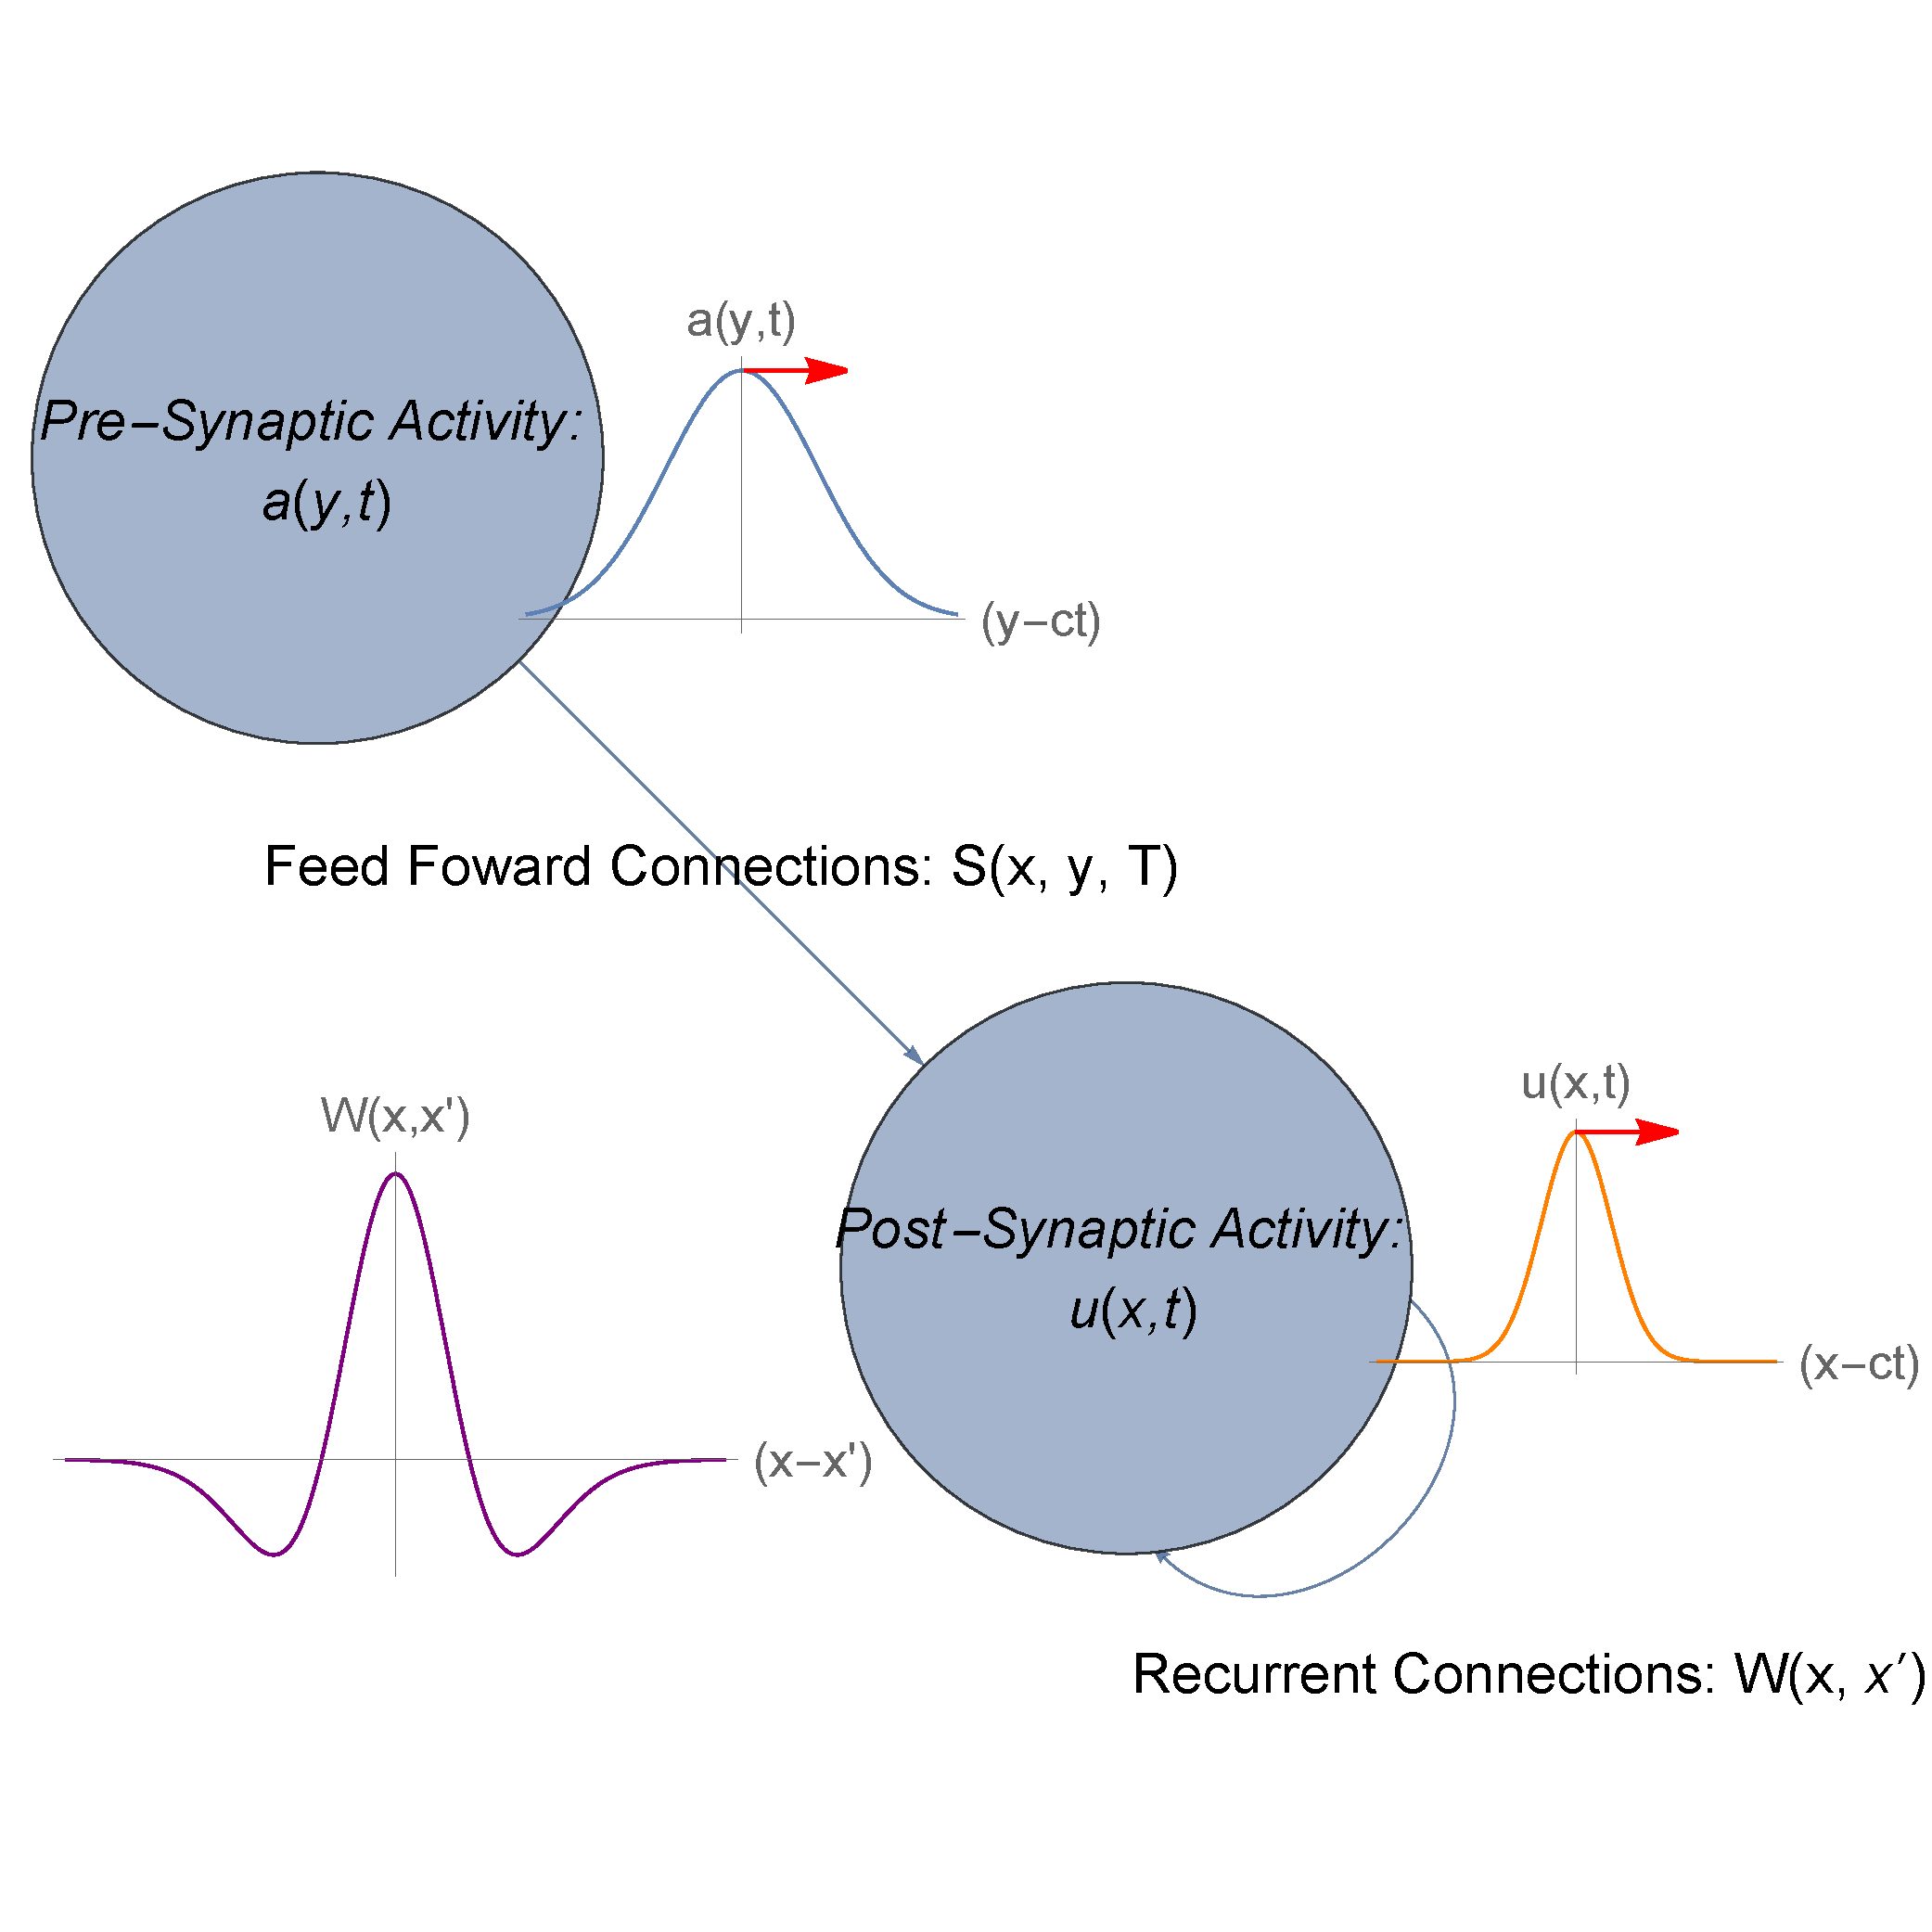
\includegraphics[width=0.7\textwidth]{images/nft_activity/model_summary}
	\def\c{The connections and directionality of the model: activity is fed-forward from the pre-synaptic region by the structure of interest and is spatial-temporally propagated by a time-differential operator and spatial convolution of inhibitory and excitatory recurrent connections. }
	\caption[\c]{\c Cartoons of typical propagating activity patterns and recurrent connections are shown but not feed-forward connections as determining these are the object of this study. The generated signal in the post-synaptic region and the driving signal in the pre-synaptic region are then convolved with a plasticity window to inform the synaptic changes on a slow time scale which is indicated by the variable $T = \epsilon t$ for some small $\epsilon$. \label{model-summary}}
\end{figure}
\paragraph{Representation of Topography}
What topography means in the continuous sense should be established. Two things should be preserved: the neighbourhood projection, and the excitatory feed-forward nature of the network. To preserve the neighbour-neighbour relation the connections, here referred to as a synaptic distribution, labelled $S$, and measured in synapses per mm$^2$,  should take the form:
\begin{equation}
	S(x,y,T) = S(|x-p(y)- \rho|, T),
\end{equation}
where $p(y)$ is some monotonically increasing function and $\rho$ is some constant to indicate that a coordinate shift still permits a topographic mapping. The excitatory feed-forward nature means that a patch of activation in the pre-synaptic field should activate a local patch of the post-synaptic field associated with its topographically projected location. Therefore, $S$ should decay quickly at infinity, be positive at the topographically projected location, and have a finite (small) radius at which it transitions to being negative. Alternatively, it can be strictly positive but quickly decaying such that it never over-powers the recurrent inhibitory connections; see Figure \ref{fig:topographicexamples}.

\begin{figure}[h!]
	\begin{subfigure}{0.4\textwidth}
		\centering
		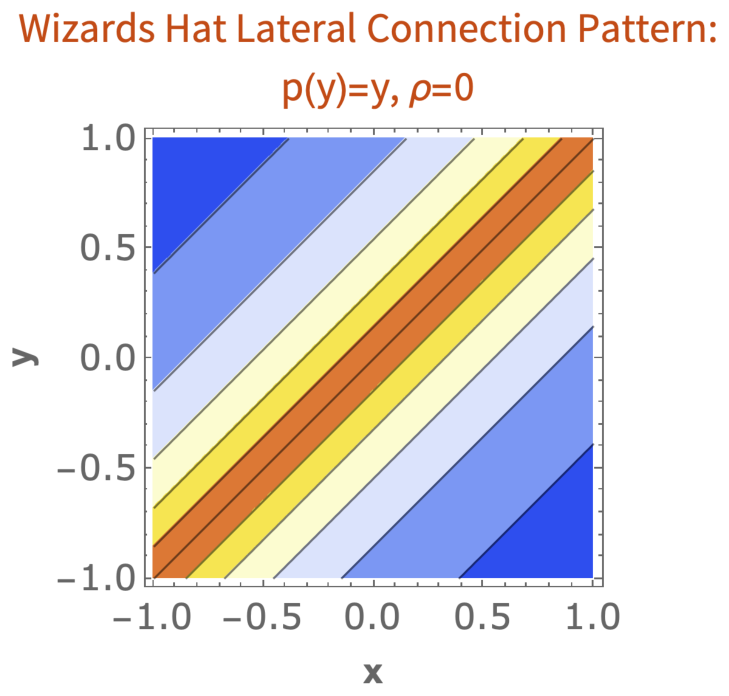
\includegraphics[width=\textwidth]{images/nft_activity/example-topographicorganisationlinear}
		\caption{}
	\end{subfigure}
	\begin{subfigure}{0.52\textwidth}
		\centering
		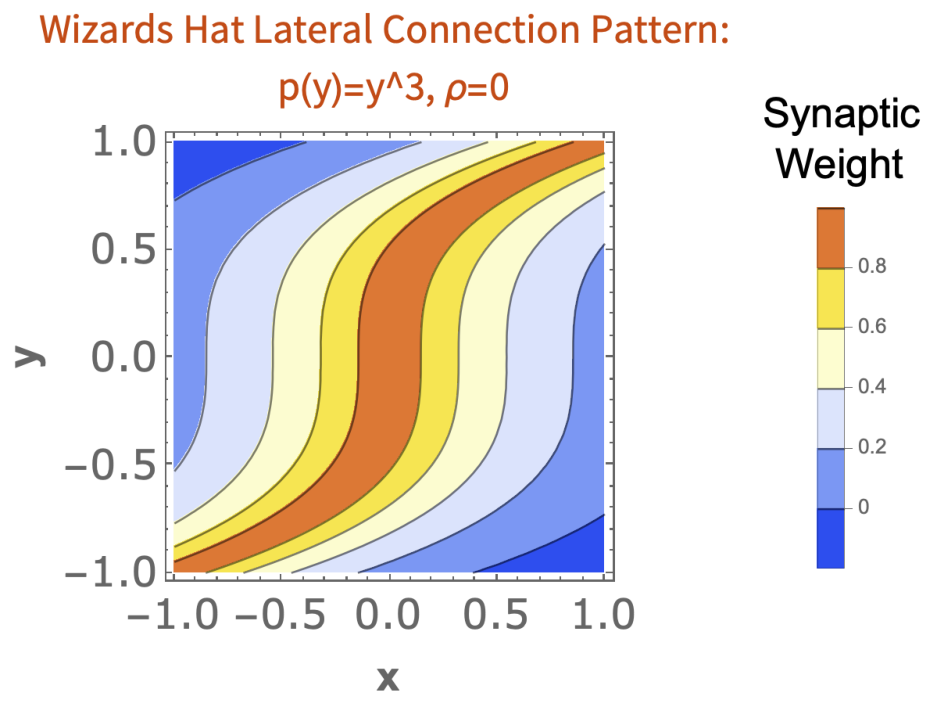
\includegraphics[width=\textwidth]{images/nft_activity/example-topgographicorganisationcubic}
		\caption{}
	\end{subfigure}
	\def\c{Two examples of topographic organisation using a Wizard hat style function: a) shows a linear relationship between axes and for while b) shows a cubic relationship between axes. }
	\caption[\c]{\label{fig:topographicexamples}  \c Both are topographic but a) has an even representation of the pre-synaptic field across the post-synaptic field while b) compresses the representation at the boundary and enlarges the interior.}
\end{figure}
\paragraph{Neural Field Theory}
The model is formed using NFT formulation proposed by Amari (1970) which considers both excitatory and inhibitory connections in the same kernel $W$ \cite{Amari1977-gc}. The pre-synaptic and post-synaptic regions are coupled by a kernel $S$. It is this kernel in which the evolution of topography is demonstrated. The electrical activity, measured in millivolts (mV), of the pre-synaptic field is denoted by $a(x,t)$ and in the post-synaptic field by $u(x,t)$, and choose the firing rate function to be a sigmoid-logistic function:
\begin{equation}
	Q(u)=\frac{Q_\text{max}}{1+\exp(-\beta(u-\theta))},
\end{equation} 
where $\beta$ and $\theta$ dictate the steepness of the curve and the threshold respectively, and $Q_{\text{max}}$ is the maximal firing rate; { the units of each are mV$^{-1}$, mV, and spikes per second and can be found in Table \ref{table:parameters}}. The activity dynamics are then governed by the internal dynamics mediated by $W$ and the input provided through the pre-synaptic field, $Q(a)$, and its transfer through $S$:
\begin{align}
	\begin{split}
		u(x,t)&
		+\tau \frac{\partial u(x,t)}{\partial t} 
		- \int_{-\infty}^{\infty} W(x, x^\prime) Q(u(x^\prime,t)) dx^\prime = \int_{-\infty}^{\infty}S(x,y, T) Q(a(y,t)) dy.
	\end{split}
	\label{eq:amari}
\end{align}
Note that the time variable $T$ is on a much slower time scale which is realised by setting $t=\epsilon T$ for $0<\epsilon \ll 1$. For the purposes of solving equation \ref{eq:amari} these connections can be considered effectively constant. A simplifying assumption is that the recurrent connections $W$ remain constant throughout the course of synaptic development and are homogenous. Following Robinson (2011) a plasticity window is defined as a rapidly decaying envelope $H$ that weights the cross-correlation of the input and response signals in a population in the same fashion as biologically-inspired plasticity rules weight individual spikes of a neuron \cite{Robinson2011-ve}. { These plasticity windows have been observed in several organisms and brain regions; a typical window has a time constant on the order of 10s of milliseconds but have been observed to be on the order of 10s of minutes \cite{Froemke2002-be, Zhang2000-lb, Allen2003-rw, Markram1997-ln, Citri2008-kv}}. The average synaptic dynamics are given by averaging over a time-window which is longer than the time-scale of the plasticity window and of the inverse frequencies of the forcing and the response stimuli but shorter than any long term plasticity changes:
\begin{align}
	\tau'\frac{dS(x,y,T)}{dT} = \int_{-\infty}^{\infty} \langle U(x,T+s)H(s)A(y,s) \rangle ds, \label{eq:robinson}
\end{align}
where $U=Q(u), A=Q(a)$ (the firing rates of the post-synaptic and pre-synaptic populations respectively), $\langle \cdot \rangle$ denotes averaging, and $\tau^\prime$ is the time-scale of synaptic dynamics. In the case of no electrical activity present in the pre-synaptic field there will be a constant level of spontaneous firing $A$ inducing an electrical activity and firing rate $U$ which in turn will lead to run-away synaptic dynamics. The dynamics of the average rate of synaptic change and the expected synaptic values are of key interest; in later sections this will be taken as an adiabatic expansion and averaging over stimulus input locations. Therefore, the above equation should include a noise term $\eta$ with strength $\kappa$ to incorporate the small deviations of spontaneous activity:
\begin{align}
	\tau^\prime\frac{dS(x,y,T)}{dT} = \int_{-\infty}^{\infty} \langle U(x,T+s)H(s)A(y,s) \rangle ds + \kappa\eta(x,y,t).
\end{align}
\paragraph{Regularisation}
Several regularisation rules have been posed to stabilise these unstable Hebbian dynamics and are broadly classified in the form of subtractive and multiplicative rules \cite{Abbott2000-gl}. A subtractive normalisation rule is chosen to stabilise the dynamics, assuming there is some atrophic factor to regulate the unbounded growth of synapses, governed by parameter $\lambda$, released at each location:
\begin{align}
	\begin{split}
		\tau^\prime&\frac{dS(x,y,T)}{dT} + \lambda S(x,y,T)=  \int_{-\infty}^{\infty} \langle U(x,T+s)H(s)A(y,s) \rangle ds + \kappa\eta(x,y,t).
	\end{split}
	\label{eq:stdpfinal}
\end{align}
The idea of a synaptic decay on the basis of metabolic demands has also been introduced in a study of organisational behaviour in V1 \cite{Wright2013-td}. The dynamics of equation \ref{eq:stdpfinal} are focused on for the remainder of this text.
\paragraph{Perturbations}
The post-synaptic field is assumed to relax in the absence of forcing activity that i.e. there is a constant level of spontaneous firing in the pre-synaptic and post-synaptic fields; note that this is not necessarily the case \cite{Coombes2005-mt}. All activity dynamics are assumed to be small perturbations from these constant rates. Furthermore, if one makes the assumption that the firing rates can be expressed as perturbations from a baseline firing rate,  $U(x,t) = U_0 + \delta U(x,t)$ and $A(x,t) = A_0 + \delta A(x,t)$, then taking Fourier transforms the average change in plasticity in the un-regularised dynamics can be expressed as:
\begin{equation}
	\frac{1}{2\pi}  \int_{-\infty}^{\infty} \delta \hat{U}(x,\omega) \hat{H}(\omega)^* \delta\hat{A}(y,\omega)^*d\omega,
\end{equation}
where $\hat{\cdot}$ denotes the Fourier transform, and $\cdot^*$ denotes complex conjugation \cite{Robinson2011-ve}. 

\paragraph{Input Stimulus}
Two classes of input stimulus are considered: mono-directional and bi-directional (radial) waves. Mono-directional waves propagate either to the left/right at speed $c$ starting at some time $t_0$ and some starting position $y_0$ finally finishing at some time $t_1$. These terms are rooted in a two dimensional consideration of the problem. A mono-directional wave might travel along a single radial angle whilst a radial wave travels isotropically. { These choices allow for a description of the waves observed in the retina  \cite{Meister1991-mu, Stafford2009, Ackman2012-uu}. Of the two the mono-directional wave is the most appropriate model but the bidirectional wave is an equivalent but analytically preferable case as shown in Section \ref{sec:monotoradial}}. Letting $r(y,t)=y-ct-y_0$, these inputs accordingly take the form:
\begin{equation}
	a(y,t) = (\Theta(t-t_0)-\Theta(t-t_1))h(r(y,t)). \label{wave:plane}
\end{equation}
Radial inputs are similar, simply propagating in both directions:
\begin{align}
	a(y,t) = \frac{(\Theta(t-t_0)-\Theta(t-t_1))(h(r(y,t))+h(r(y,-t)))}{2}. 
	\label{wave:radial}.
\end{align}
In both cases $h$ is used to denote the shape of the propagating wave-form. The choice of $h$ is left to be general but can be thought of as a travelling Gaussian wave-packet. A function may be approximated by a linear sum of appropriately weighted Gaussian's and so this forms a basis set and the simple case is considered in Section \ref{sec:param}.
\paragraph{Plasticity Windows}
There are two general forms of plasticity considered: time symmetric and time asymmetric plasticity. Time symmetric plasticity, also called Correlation Dependent Plasticity (CDP), means that connections are strengthened by spikes that are separated by short times and weakened by medium-long time separated spikes, but in which the ordering of the spikes is not important. Time asymmetric plasticity, or STDP, means that not only does the temporal closeness of pre-synaptic and post-synaptic spikes matter but the ordering in which they occur: post-synaptic firing that occurs before pre-synaptic firing weakens the connection and vice-versa. A canonical form of these two rules expressed as a plasticity envelope is given by:
\begin{equation}
	H(s) = \begin{cases}
		A_+\exp(-\frac{s}{t_p}) \quad &s\geq 0\\
		A_-\exp(\frac{s}{t_p}) \quad &s <0
	\end{cases}
\end{equation}
where $A_-=A_+$ for CDP and $-A_-=A_+$ for STDP, and $t_p$ is the time-scale of the plasticity \cite{Abbott2000-gl}. The Fourier transforms of these learning rules are:
\begin{align}
	\hat{H}_{CDP}(\omega) &= \frac{2A_+}{1+\omega^2 t_p^2} \label{rule:CDP}\\
	\hat{H}_{STDP}(\omega) &= \frac{2A_+\omega it_p}{1+\omega^2 t_p^2} \label{rule:STDP}
\end{align}
In summary, a membrane signal is generated in the post-synaptic region on a fast-time scale which is supported by recurrent connections and generated by input from a pre-synaptic region. The spatial-temporal patterns of the pre-synaptic and post-synaptic activity then inform synaptic changes between the two regions on a slow time scale in accordance with a plasticity rule.

\section{Analysis}
The connectivity kernels, pre-synaptic stimuli, and post-synaptic activity and firing rates are assumed to be elements of Schwartz space i.e. the functions and derivatives that define these rates decay quickly at long range and they are localised. This assumption is made to ensure bio-physical realism. Connectivity kernels typically have short-range and long-range interactions but they do not interact at all with very distal connections and their functions must accordingly decay at infinity. Similarly, due to these recurrent connectivity kernels, electrical signals only seem to be able to support themselves on finite distances and they too must accordingly decay. The assumption of Schwartz functions ensures the Fourier transforms existence and makes formulating the problem in Fourier space desirable.

\paragraph{Approximating Input Stimulus}
The inputs specified earlier are biologically realistic but will become more tractable if one of the Heaviside functions can be removed; this would amount to a stimulus propagating to infinity after being initialized. This approximation can be made if the synaptic change induced by this different stimulus is arbitrarily small when compared to the synaptic change induced by the true stimulus. This is realised by the rapid decay of the plasticity window and shown formally in Lemma \ref{lemma:decay}; see Appendix A.

\paragraph{Activity Dynamics}
It was reasoned on physical grounds that in the absence of pre-synaptic stimulation the only post-synaptic solution is a static, constant level of activity. Synaptic dynamics are governed by perturbations from this baseline and expressions for these are derived in this section. The baseline is assumed to be sufficiently close to the origin that the logistic function is analytical and has a convergent Taylor series expanded around $u = u_0$. Therefore, a good approximation is:
\begin{equation}
	Q(u) = Q(u_0) + u Q'(u_0). \label{eq:firingapproximation}
\end{equation}
This can then be inserted in equation (\ref{eq:amari}) and a Fourier transform can be taken to yield:
\begin{align}
	\hat{u}(k,\omega) = Q&(u_0)\Gamma(k,\omega)(\hat{W}(k)+\hat{S}(k))\delta(k)\delta(\omega) + Q'(u_0)\hat{S}(k)\Gamma(k,\omega)\hat{a}(k,\omega),
\end{align}
where $\Gamma(k,\omega)=(1 + i\tau\omega - \hat{W}(k))^{-1}$. Now, recognising that $Q(u_0)\Gamma(\omega,k)(\hat{W}(k)+\hat{S}(k))\delta(k)\delta(\omega)$ corresponds to the static solution, i.e. the baseline activity level, the expression for the Fourier transform of the perturbation of the activity level is: 
\begin{equation}
	\delta\hat{U}(k,\omega) =\hat{S}(k)\Gamma(k,\omega)\hat{a}(k,\omega),
\end{equation}
where $U(x,t)=Q(u(x,t))$. The Fourier Transform of the perturbation from the baseline rate in the pre-synaptic field, $\delta A(y,t)$ is trivial to compute: $ \delta \hat{A}(k,\omega)=\delta \hat{a} (k,\omega)$. This is sufficient to explicitly compute the synaptic change between any two points in the pre-synaptic and post-synaptic field. 
\paragraph{Synaptic Dynamics}
The synaptic field, and synaptic changes are assumed to be isotropic; $S(x,y,T) = S(x-y,T)$ for all $T$. Then, making the approximation of the firing rate, and taking spatial Fourier transforms the synaptic change can be written:
\begin{equation}
	\delta(p+k)\frac{d\hat{S}(k,T)}{dT} = \delta(p+k)(S_0 - S_1 \hat{S}(k,T)) +  S_2\int_{-\infty}^{\infty}  \hat{a}(\omega,p)\hat{a}(\omega,k)^* \hat{H}(\omega)^* \hat{S}(k,T)^*\Gamma(\omega,k)  d\omega ,
\end{equation} 
where $S_0$, $S_1$, and $S_2$ have absorbed the time constant, regularisation constants, baseline firing rate, and the Fourier normalisation terms. The sign of $S_1$ is negative to indicate its relationship with the decay constant $\lambda$. Integrating with respect to $p$, the above equation may be solved as:
\begin{align}
	&\frac{d\hat{S}(k,T)}{dT} = S_0 - S_1\hat{S}(k,T) + S_2\hat{S}(k,T)^*\int_{-\infty}^{\infty}\mathcal{B}(\omega)\hat{a}(\omega,k) \hat{H}(\omega)^* \Gamma(\omega,k) d\omega,
\end{align}
where $\mathcal{B}(\omega) =  \int_{-\infty}^{\infty} \hat{a}(\omega,p)^*dp$. The connectivity kernel $S$ in position space is physically required to be real. This kernel is written as the composition of odd and even functions. Then, from conjugate symmetry it follows that its Fourier transform is composed of a real part consisting of the linear combination of the Fourier transforms of its even components, and an imaginary part consisting of the linear combination of the Fourier transforms of its odd components. For $S$ to remain real its derivative must have an even function as its real component, and an odd function as its imaginary component. Let,  
\begin{equation} 
	G(k)= \int_{-\infty}^{\infty} \left(\int_{-\infty}^{\infty}  \hat{a}(p,\omega)^*dp\right)\hat{a}(\omega,k) \hat{H}(\omega)^* \Gamma(k,\omega) d\omega.
\end{equation}
If $G(k)$ is even and real, or odd and purely imaginary, then the above equation can be separated into odd and even parts and solved as two independent ODEs. Attention will be restricted to the even form of $G(k)$ for reasons detailed in the following section. Denoting $S_{O}(x,T)$ and $S_E(x,T)$ to be the odd and even parts of the coupling function in position space these ODEs are then: 
\begin{align}
	&\frac{d\hat{S}_O(k,T)}{dT} =-(S_1 + S_2 G(k)) \hat{S}_O(k,T) \\
	&\frac{d\hat{S}_E(k,T)}{dT} = S_0 + (S_2 G(k) - S_1) \hat{S}_E(k,T) .
\end{align}
Therefore, in the asymptotic limit, provided $S_1 + S_2 G(k)>0$, the odd components of the initial organisation decay to zero and provided $S_1 > S_2 G(k)$ the even components have solution:
\begin{equation}
	\hat{S}_E(k) = \frac{S_0}{S_1 - S_2G(k)}. \label{eq:asymptoticsynapse}
\end{equation}
The final organisation is therefore dictated by the initial even components and the form of $G(k)$. $G(k) > 0$  is sufficient to satisfy the above conditions and this will be accordingly shown. The form of $G$ is prescribed by the learning rule employed and the input stimulus used and referred to as the training function.

\paragraph{Mono-Directional Propagation} \label{sec:monotoradial}
Supposing the input stimulus is $a(y,t) = \Theta(t) h(y-ct-y_0)$ it is fairly straightforward to show that the training function $G$ is not even and therefore will not work as a training function. However, assuming that the synaptic changes are adiabatic or reasonably small and assuming the proportions of waves propagating left and right are equal then the average synaptic dynamics induced by inputs of the mono-directional form (equation \ref{wave:plane}) are the same as the dynamics induced by inputs of the radial form (equation \ref{wave:radial}). Attention is therefore restricted to radially propagating inputs.
\paragraph{Radial Propagation}
Presume the input stimulus is in the form $a(y,t) = \Theta(t) (h(y-ct-y_0)+h(y+ct-y_0))$. Taking two Fourier transforms yields:
\begin{align} 
	\begin{split}
		\hat{a}(p,\omega)& = \frac{1}{2} e^{-2\pi i y_0 p}\hat{h}(p) \left( \delta (w+cp) + \delta (w-cp) + \frac{2iw}{\pi (w-cp)\pi (w+cp)}\right).
	\end{split}
\end{align}
Integrating with respect to $p$ by using the Cauchy Residue Theorem and evenness of the last term and $\hat{h}$ gives:
\begin{equation} 
	\label{integrateap}
	\int_{-\infty}^{\infty}\hat{a}(p,\omega)^*dp = \left(1 + \frac{2}{c} \right) \hat{h}\left(\frac{\omega}{c}\right)^* \cosh\left(2\pi i y_0 \frac{\omega}{c}\right).
\end{equation}
$G(k)=G(k; y_0)$, assuming the synaptic changes at each time step are small, the average synaptic change can be written as:
\begin{equation}
	\left \langle \frac{d\hat{S}(k,T)}{dT} \right \rangle = S_0 - S_1\hat{S}(k,T) + S_2 \hat{S}(k,T) \langle G(k; y_0, c) \rangle. 
\end{equation}
The asymptotic limit, which is the target of this work, will approach this average and for the remainder of this work angle brackets are dropped. Let $g(k;c) = (\hat{H}(ck)^* \Gamma(k,ck)+\hat{H}(-ck)^* \Gamma(k,-ck))/c$. Equation (\ref{integrateap}) can then be inserted into the expression for $G(k)$ and the Dirac-Deltas can be integrated. Then, $y_0$ is integrated out by assuming it is distributed over some interval of length $L$ giving exponential integral functions which vanish as $y_0 \rightarrow \infty$ yielding:
\begin{equation}
	\frac{d\hat{S}(k,T)}{dT} = S_0 + \hat{S}(k,T)\left(S_2 g(k;c) |\hat{h}(k)|^2 - S_1 \right), \label{eq:finalsyn} 
\end{equation}
Showing that $g(k;c)$ is even may be done by direct substitution for both STDP and CDP rules under the assumption that both $W$ and $h$ are even. It follows that all $G(k)$ are even. It remains to be shown that $G(k)$ is restricted to being non-negative or non-positive. All the scaling constants are positive and it is therefore clear for the STDP rule that $G(k)\geq 0$, while for the CDP rule $G(k)$ is never non-positive and is only non-negative if $\hat{W}(k)<1$. It is certainly possible that this is the case, but it is not true for common choices of $W$. $W$ is typically chosen to be in the form of a ``wizard-hat" with short-range excitation and long range inhibition which is theoretically grounded and observed experimentally \cite{Sirosh1994-zv, Phongphanphanee2014-in}.
\subsection{Computational Analysis and Parameter Estimation}
There has been little reference to the recurrent connections or input stimulus (with the exception of wave-speed $c$) and the parameters and functional forms that characterise them. These will now be explicitly defined and the consequences of this choice examined by computational means. Key parameters of the model contributing to width (arbor size) will be estimated by means of Markov Chain Monte Carlo (MCMC) applied to wild-type and $\beta2^{-/-}$ mutant data. This estimation allows for both model validation and estimation of biological quantities which have not yet been experimentally examined.

The wave-form of the input stimulus is modelled as a Gaussian with amplitude and width (variance) parameters of $\sigma_1$ and $\sigma_2$ respectively and with Fourier Transform $\hat{h}(k) = \sigma_1 \sigma_2\exp(-k^2\sigma_2^2/2)$. The recurrent connections are described by a difference of two Gaussians: $\hat{W}(k) =  r_1\exp(-k^2 r_1^2/2) -  R_1r_2\exp(-k^2 r^2)$. This choice ensures that the dimensional requirements for the propagator are satisfied and that $|W(k)|<1$ for a suitable choice of recurrent connection parameters. These choices mean that there are 16 key biological parameters: $u_0, \tau, \tau^\prime, \kappa, \lambda, A_p, t_p, Q_\text{max}, \beta, \theta, $\\$c, \sigma_1, \sigma_2, R_1, r_1, r_2$.

\paragraph{Parameter Analysis} \label{sec:param}
Examination of equation \ref{eq:asymptoticsynapse} shows that $S_0$ (or $\kappa/\tau^{\prime})$ serves to stabilise the dynamics at the cost of introducing noise - the Fourier spectrum of a biologically realistic organisation will decay to a constant i.e. to a baseline level of white noise. A tolerable level of system noise is expected and it is assumed that this noise can be filtered by some means. The denominator dictates the deviations from this noise and noting that for both CDP and STDP $G(k) \rightarrow 0$ and $G(k)>0$ ensures that physically viable solutions enforce $0<G(k)<S_1/S_2$ and non-viable solutions contain pairs of singularities (via evenness of $G$) where $G(k)>S_1/S_2$ for some $k$. 

An arbitrarily large wave-amplitude $\sigma_1$ can force a singularity in both cases and an arbitrarily large $c$ can force a singularity in the STDP case. Therefore, stability in the STDP case that the maximum wave speed is bound by a contour inversely proportional to wave-amplitude and vice-versa. Given the likely biological restrictions on amplitude this implies that wave speed could be dictated in part by wave amplitude. With this in mind $\sigma_1$ is set to $5$mV for the remainder of this work. This ensures that there is a baseline distinguishable level of firing when the wave reaches its peak amplitude but the neurons are not near a saturated level thus satisfying the assumptions required for the approximation in equation \ref{eq:firingapproximation}. The parameters $u_0, \tau^\prime, \lambda, A_p, f_\text{max}, \beta, \theta$ are absorbed into $S_0, S_1$, and $S_2$ and their effects on the dynamics are immediate: they dictate the absolute measurable values of the organisation, not the form. These parameters are set according to Table \ref{table:params} for the remainder of this work.

\begin{table}[h!]
	\centering
	\begin{tabular}[width=0.5\textwidth]{| l || l | l | l |}
		\hline
		Param. & Value & Units  & Description \\
		\hline
		$u_0$ & -58 & mV & Resting potential \\
		$\tau$  & 0.1 & s & Activity time-scale \\
		$\tau^\prime$  & 100 & s & Synaptic time-scale \\
		$\kappa $  & 0.001 & syn.mm$^{-1}$ & Synapse density \\
		$\lambda $  & 0.001 & $-$ & Decay rate\\
		$A_p $  & 1 & syn.mm$^{-1}$  s & Hebbian rate\\
		$t_p $  & 1.0 & s  & Hebbian time-scale\\
		$Q_\text{max} $  & 1 & s$^{-1}$   & Max firing rate\\
		$\beta$ & 0.26 & mV$^{-1}$ & Rate steepness\\
		$\theta$ & -45 & mV & Rate threshold\\
		$c$ & 0.1 & mm s$^{-1}$ & Wave-speed\\
		$\sigma_1$ & 5 & mV & Wave-amplitude\\
		$\sigma_2$ & 0.1 & mm & Wave-length\\
		$R_1$ & 1.08 & syn.mm$^{-1}$ &Recurrent amplitude\\
		$r_1$ & 0.129 & mm &Inhibitory length-scale\\
		$r_2$ & 0.136 & mm &Excitatory length-scale\\
		\hline
	\end{tabular}
	\def\c{Choices for the biological parameters used in a neural field theory model of topographic development. }
	\caption[\c]{\label{table:params} The choices made for each of the biological parameters used throughout the chapter, unless otherwise stated. The length scale is chosen to reflect the scale at which NFT typically applies in the brain and the appropriate scale for the mouse SC \cite{Robinson2005-en}. The resting membrane potential, the threshold voltage, and the voltage scale are estimated to be in line with electrophysiological recordings \cite{Shi2018-er}. These parameters should be carefully measured if a specific biological system is to be closely analysed. \label{table:parameters}}
\end{table}

CDP $G(k)$ attains its global maximum at $k=0$ meaning that its stability is determined entirely by the relationship between $S_1$ and $S_2$. Furthermore, with CDP synaptic changes have the potential to be overly large with no parameter available to mitigate them. In the STDP case the small timescale ensures that the changes are small and the adiabatic assumption is satisfied. Attention is now restricted to the STDP case noting that extending the analysis to a CDP rule would be straightforward but care must be taken in the choice of parameters.

These choices, while considered, have reduced the problem to a single learning rule and several key parameters. It should be stressed that the other parameters must be carefully measured for accurate predictions and are in some sense non-trivial: one can manipulate them biologically and cause a bifurcation in the organisation dynamics. Figure \ref{fig:stablity} demonstrates the manifold in the $c-\sigma_2$ plane for which the model presents plausible (stable) solutions. Only a 2-dimensional slice of the overall manifold for which there are no solutions with singularities is shown, but care should be taken in ensuring that any solution of interest lies within the volume of this manifold for all parameters.
\begin{figure}
	\centering
	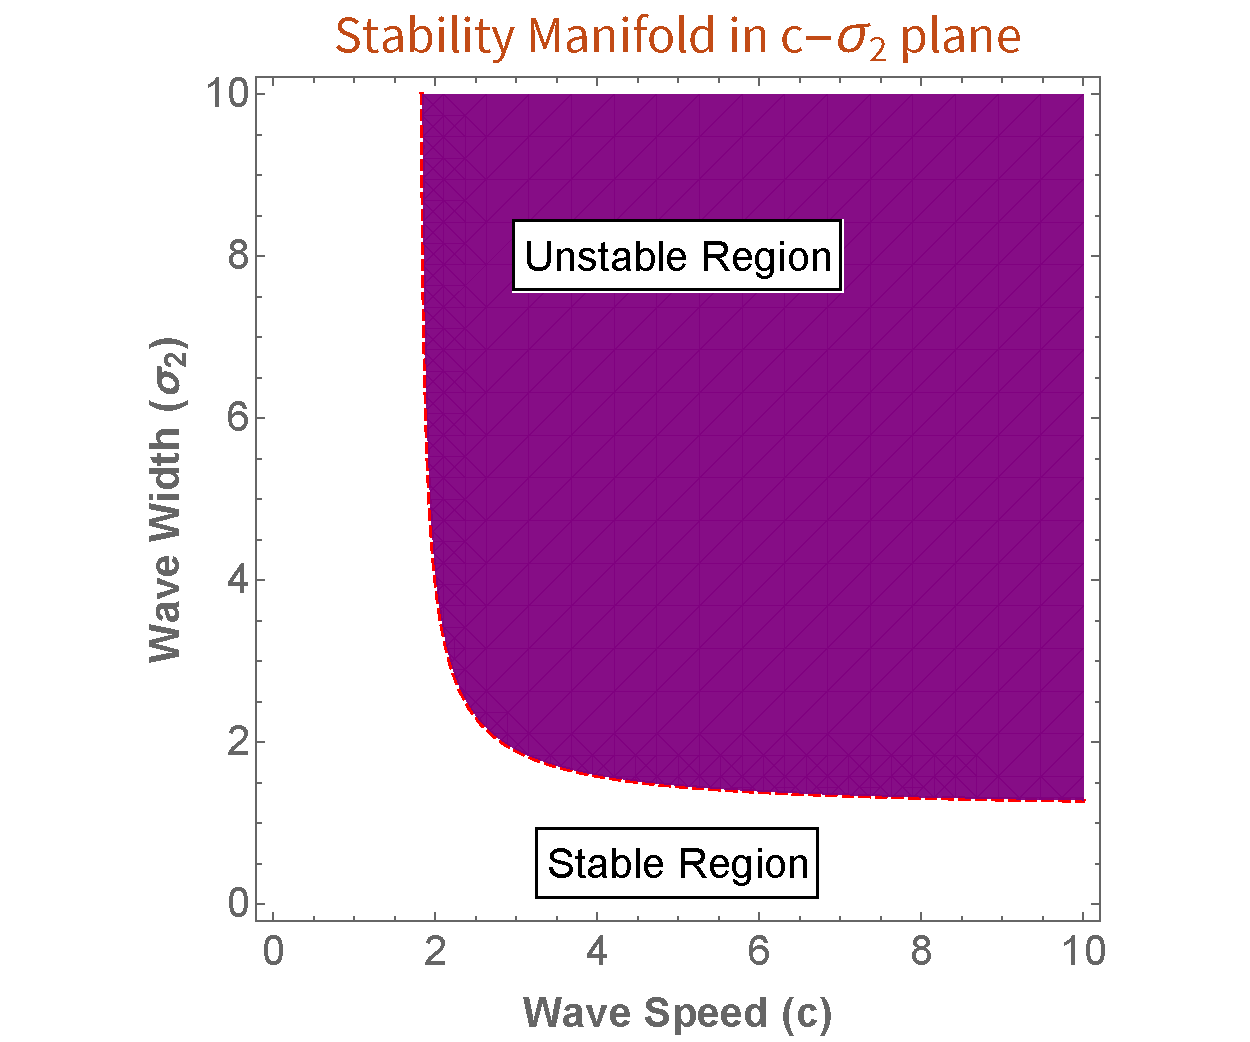
\includegraphics[width=0.75\textwidth]{images/nft_activity/stabilitysurface}
	\def\c{The manifold in $(c,\sigma_2)$ space which defines the stability of the final organisation. }
	\caption[\c]{\label{fig:stablity} \c Below the surface solutions do not exhibit singularities and the training function is deemed to be stable; in general, small choices for the parameters exhibit stable synaptic organisations at the cost of arbitrarily small amplitude. The manifold appears to be well-above reasonable estimates for these parameters, ensuring the model is likely stable in plausible biological scenarios.} 
\end{figure}
\paragraph{Fourier Space}
{  The Fourier transform of $S$ has a characteristic bump near the origin which decays to a constant representing a baseline level of noise  i.e. $\hat{S}(k) = c_0 + \hat{\mathcal{S}}(k)$ where $\hat{\mathcal{S}}(k)$ is a symmetric function decaying quickly to zero.} Note that it is possible for $\hat{\mathcal{S}}(k)$ to fall below the noise level which implies that the system will be out of phase and suppress signals at this wave length. A typical representation in Fourier and real space is shown in Figure \ref{fig:powerdistribution}a. 
\begin{figure}
	\centering
	\begin{subfigure}{0.4\textwidth}
		\centering
		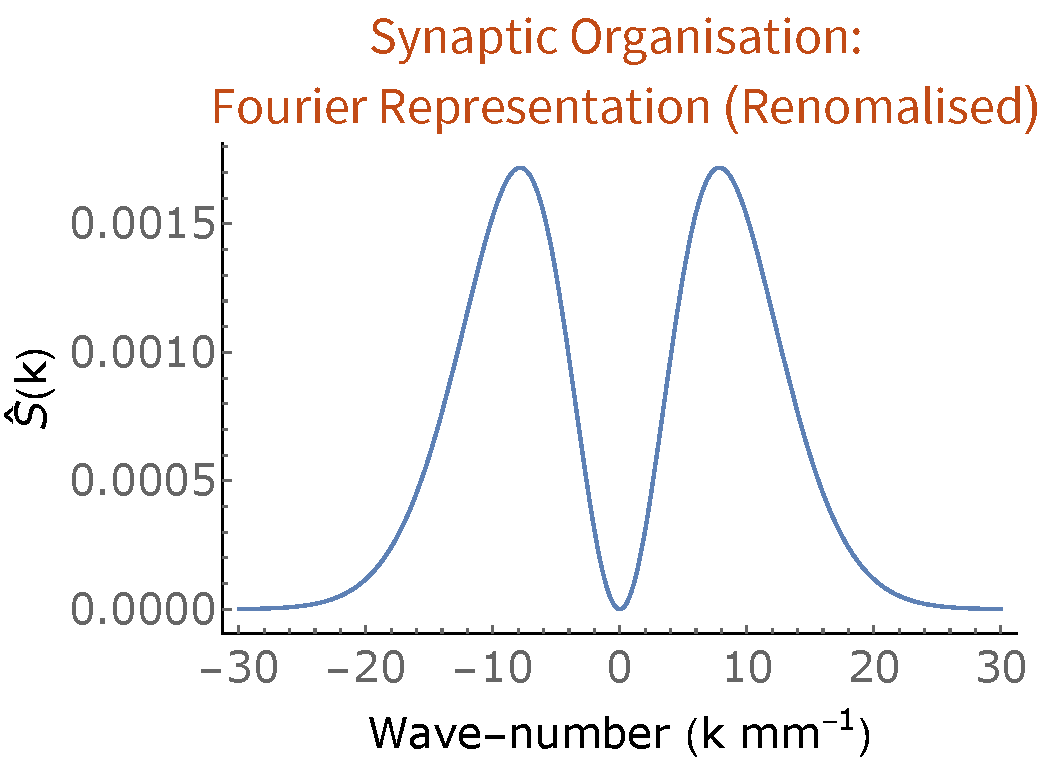
\includegraphics[width=\textwidth]{images/nft_activity/example-typicaldistributionfourier}
		\caption{}
	\end{subfigure}
	\begin{subfigure}{0.4\textwidth}
		\centering
		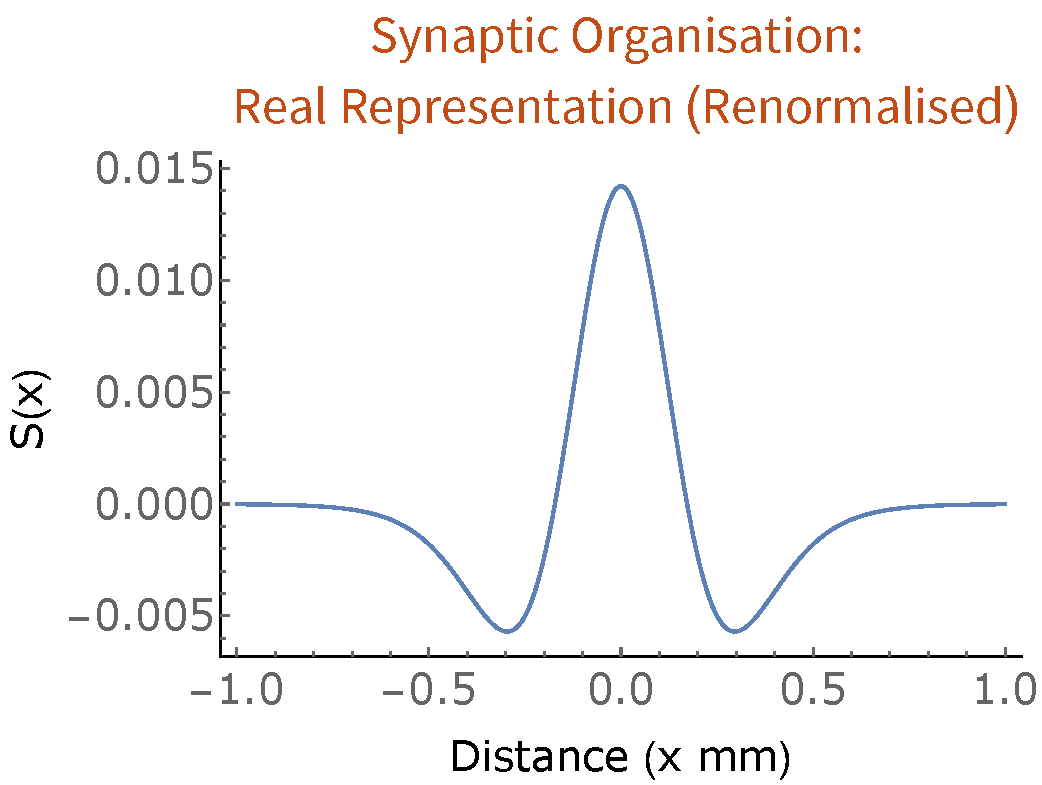
\includegraphics[width=\textwidth]{images/nft_activity/example-typicaldistributionreal}
		\caption{}
	\end{subfigure}
	\def\c{A typical organisation generated with the parameters shown in Table \ref{table:parameters} with (a) showing the representation in Fourier space, and (b) the representation in real space after re-normalisation. }
	\caption[\c]{\label{fig:powerdistribution} \c} 
\end{figure}

The distribution of the connections in physical space can be found by inverting its Fourier representation which presents a problem with the inclusion of the Dirac-Delta distribution introduced by $c_0$. This problem can be circumvented by realising that the baseline constant representation of all frequencies represents white noise which can be therefore be renormalised and omitted; see Figure \ref{fig:powerdistribution}b. This re-normalisation is done under the assumption that provided the amplitude of $\hat{\mathcal{S}}(k)$ provides a high enough signal-to-noise ratio then this system will be absorbed into already present biological noise which is filtered out in downstream calculations.
\paragraph{Refinement}
The steady state solution of the synaptic distribution $S$ takes its maximum at the origin and rapidly decays at large distances. The distributions feed-forward capability is therefore dictated by the magnitude at the origin and the rate of the decay. For precise signal transmission (or a refined retinotopy) the width of the distribution should be small with respect to the length scale. Width is estimated by taking the inverse of the wave-length that maximises the power spectrum:
\begin{equation} \label{eq:width}
	\Omega(\vec{\rho}) =  \frac{1}{\text{argmax}_k\left| \hat{S}(k;\vec{\rho})\right|},
\end{equation}
where $\vec{\rho}$ represents the vector of parameters which define the model. The width relationships in the plane of several pairs of variables within a stable region containing no singularities are examined and shown in Figure \ref{fig:parametereximinations}. Refinement tends to decrease in accordance with decreases in $c, \sigma_2, (r_1/r_2), R_1, t_p$, and $\tau$. On the biological scales of interest for the current work the decreases do not appear to be substantial in the $R_1$ and $\tau$ directions. In general the relationships between the variables are non-linear.

\begin{figure*}[h!]
	\centering
	\begin{subfigure}{0.45\textwidth}
		\centering
		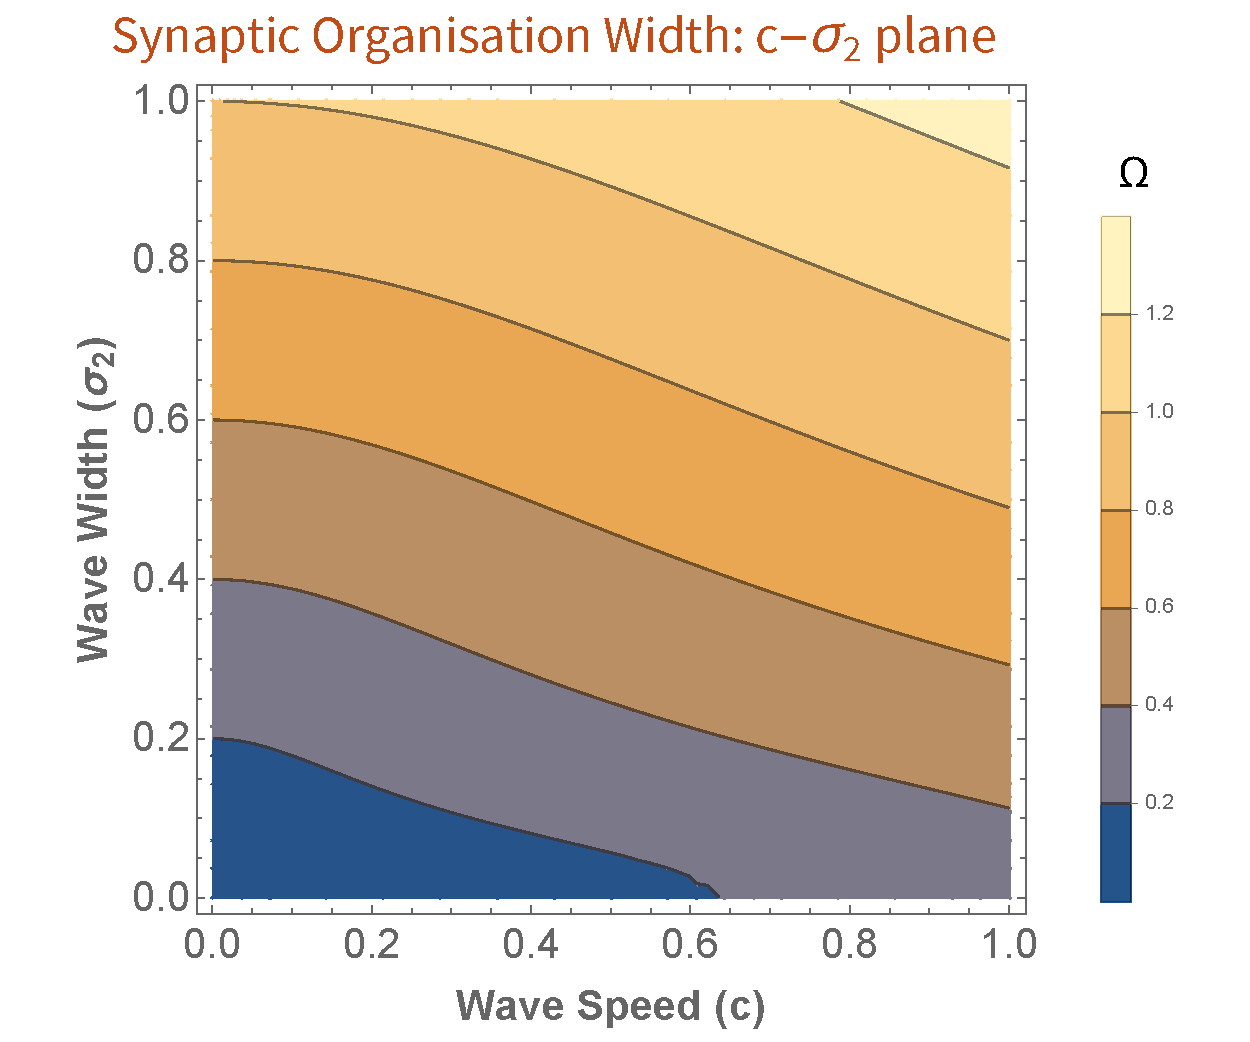
\includegraphics[width=\textwidth]{images/nft_activity/width_cs2}
		\caption{}
	\end{subfigure}
	\begin{subfigure}{0.45\textwidth}
		\centering
		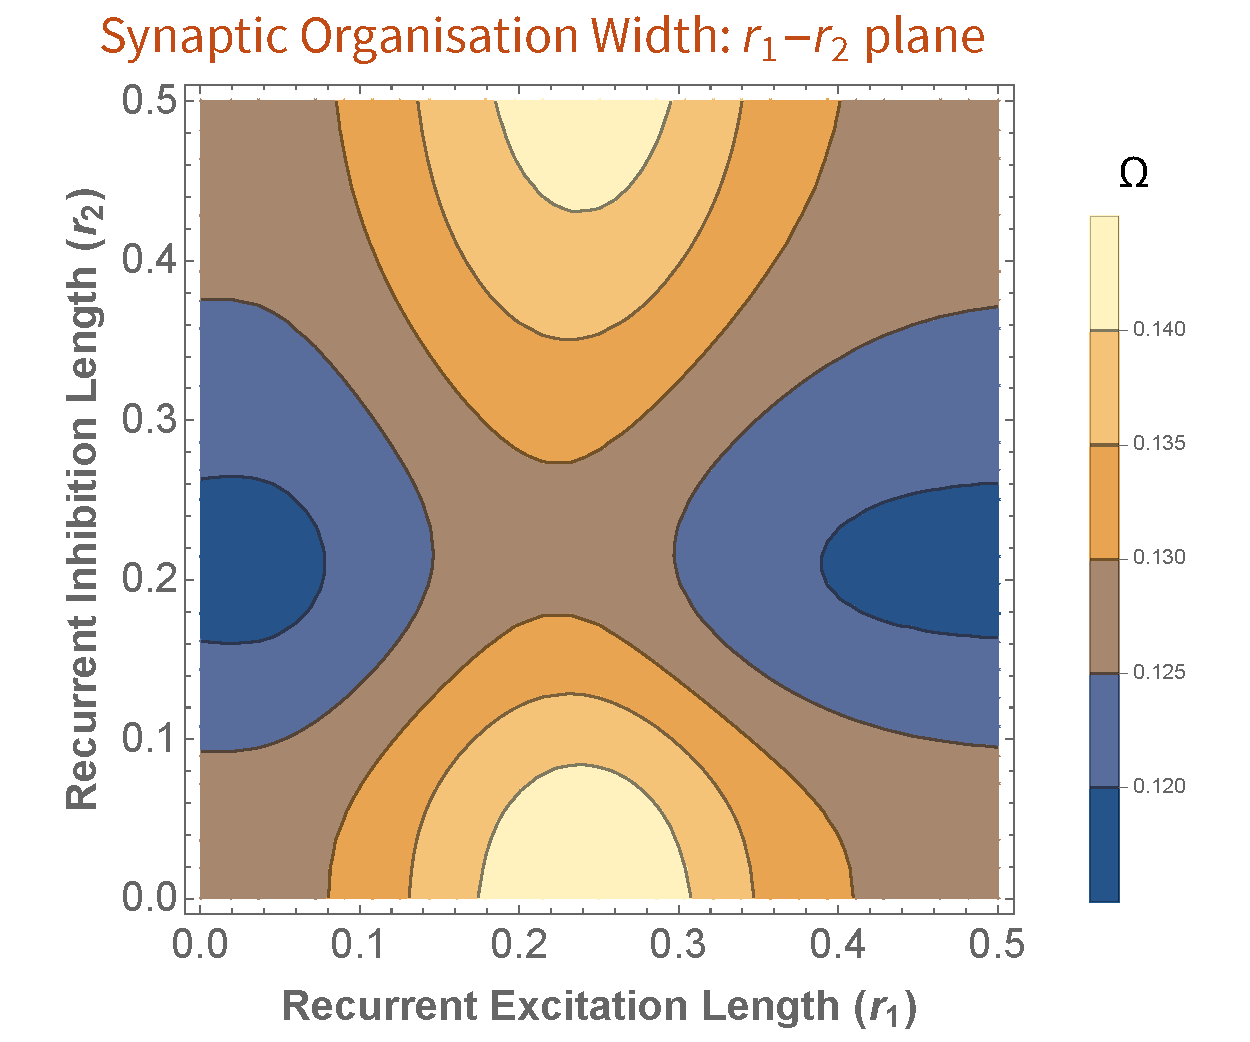
\includegraphics[width=\textwidth]{images/nft_activity/width_r1r2}
		\caption{}
	\end{subfigure}
	\begin{subfigure}{0.45\textwidth}
		\centering
		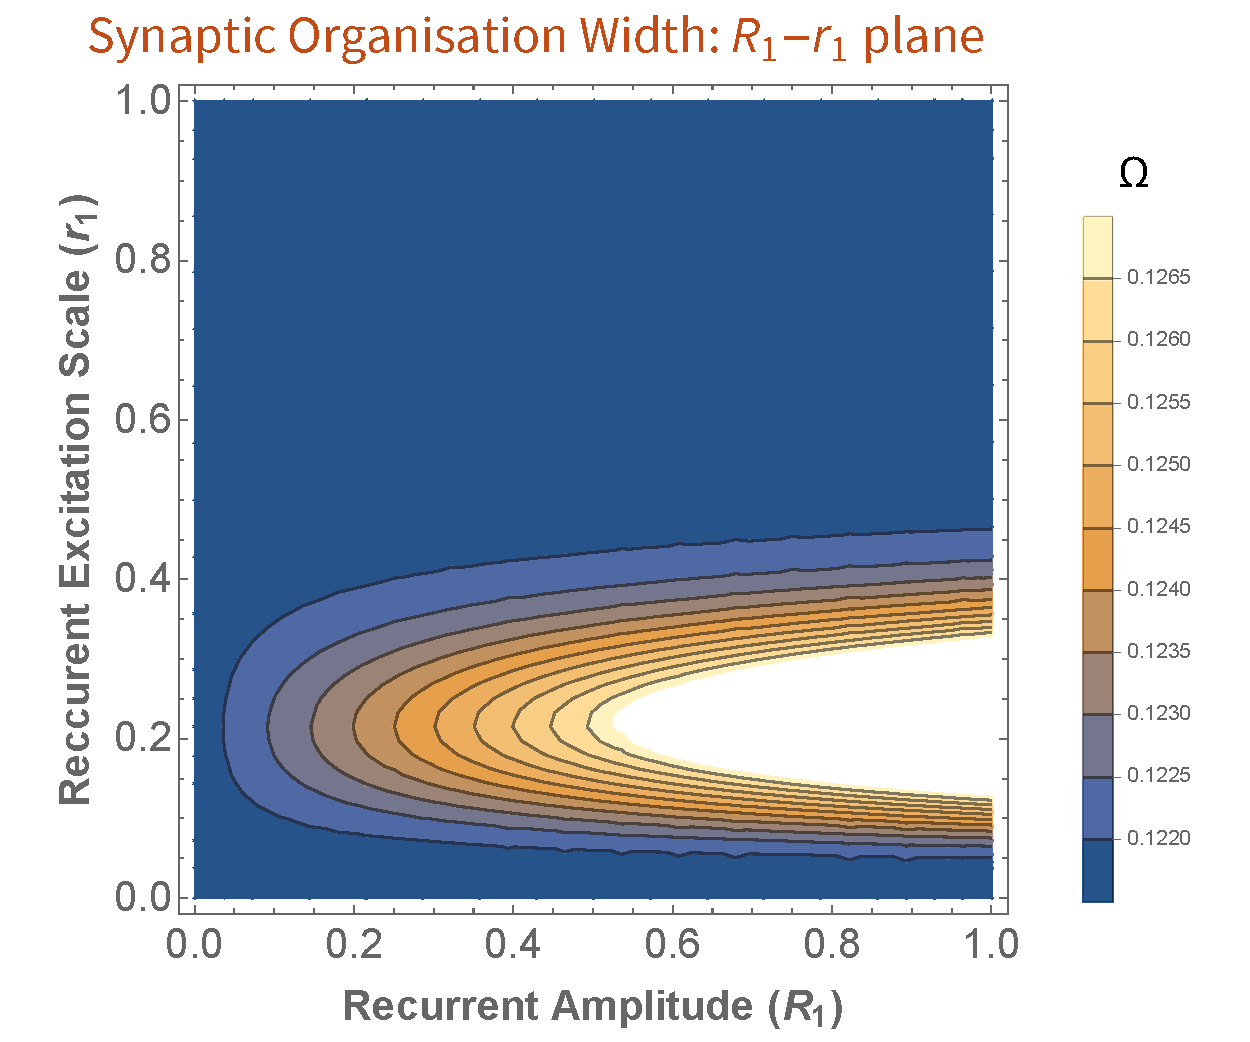
\includegraphics[width=\textwidth]{images/nft_activity/width_R1r1}
		\caption{}
	\end{subfigure}
	\begin{subfigure}{0.45\textwidth}
		\centering
		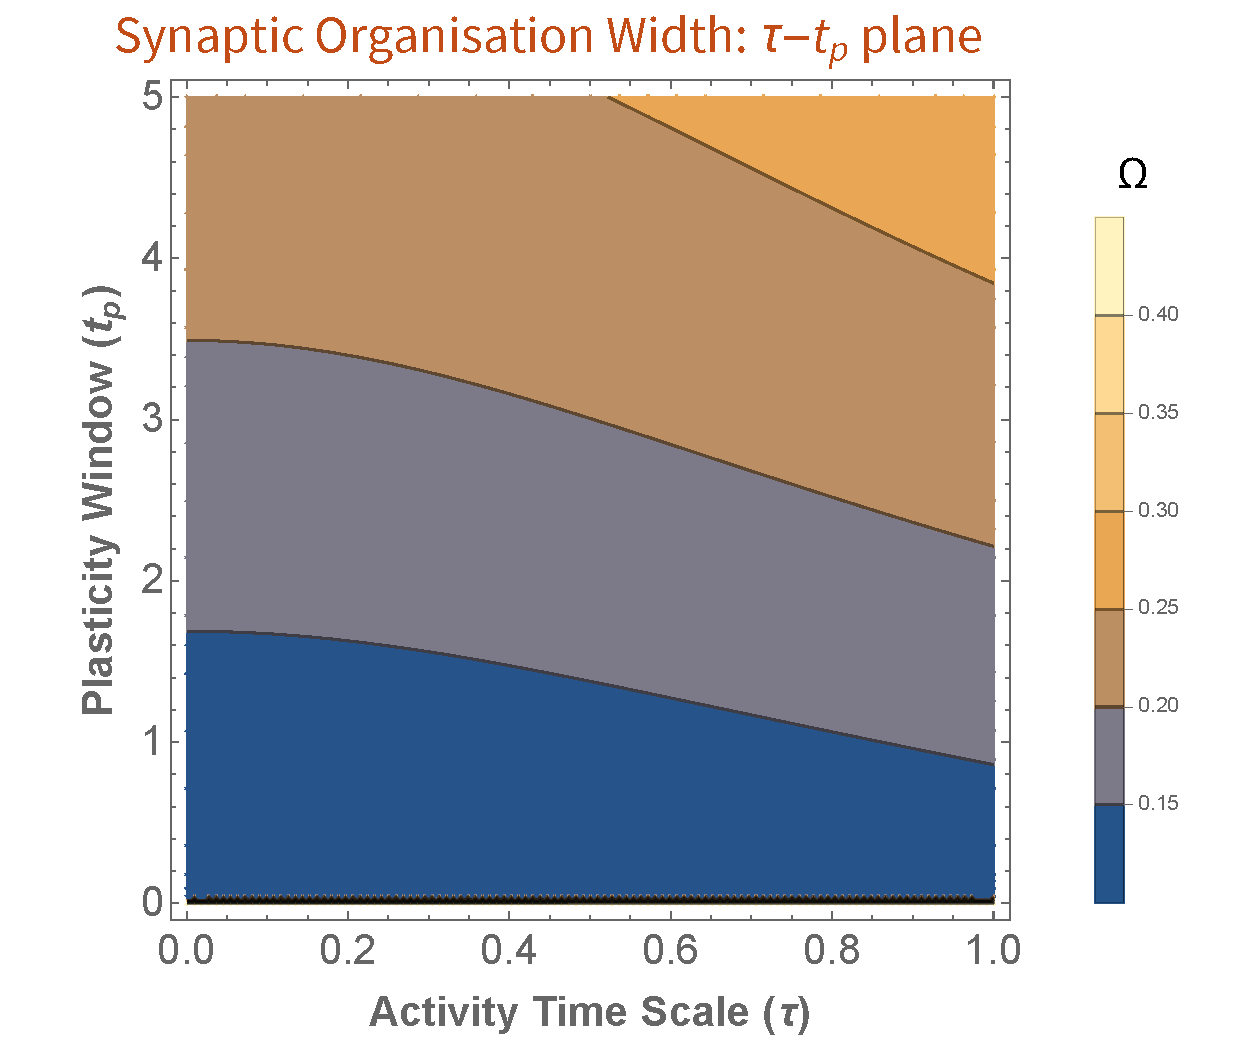
\includegraphics[width=\textwidth]{images/nft_activity/width_tautp}
		\caption{}
	\end{subfigure}
	\def\c{The variation in width ($\Omega$) in four distinct planar slices of the manifold of parameters which influence the models prediction of mean distribution width. }
	\caption[\c]{\label{fig:parametereximinations} \c Panel (a) shows that width decreases both with wave-speed and wave-width, qualitatively accounting for the differences between the wild-type and $\beta2^{-/-}$ mutant. Panel (b) shows that width decreases with with the ratio of excitation to inhibition in the recurrent connections $W$ suggesting a smaller zone of excitatory support decreases arbor size. There is an anti-symmetry along the line $r_1 = r_2$ which is expected as the dominant connection type switches along this line.  Panel (c) shows that width decreases with recurrent connection amplitude but the effect is not substantial. Panel (d) shows that width predominately decreases in accordance with the plasticity window time-scale, and while the activity time-scale has an effect it is not substantial.}
\end{figure*}

\paragraph{Sensitivity}
{ In the context of refinement it is prescient to consider which parameters affect the models prediction of the width $\Omega$ in equation \ref{eq:width}. This width will satisfy $dS(k; \vec{p})/dk = 0$ which inserted into equation (\ref{eq:asymptoticsynapse}) yields:}
\begin{equation}
	\frac{dg(k; \vec{p_g})}{dk} = 0,
\end{equation}
where $\vec{p_g} = \{c, \tau, t_p, \sigma_2, R_1, r_1, r_2\}$. The width will only vary in accordance with these parameters which is confirmed by numerical simulation.


\paragraph{MCMC Parameter Estimation}
The $\beta2$ knock-out in mouse has the effect of broadening the spatio-temporal patterns of spontaneous activity in the retina and SC during development \cite{ Stafford2009}. The mutant mice have substantially wider arborisations than in wild-type establishing the importance of activity in refining the retinotopic projection \cite{Dhande2011-jp}. Existing models have not been able to predict this wider arborisation when the patterns of activity associated with the knock-out are replicated in the model's mechanisms for activity \cite{Lyngholm2019-fs}.

\begin{figure*}[h!]
	\centering
	\begin{subfigure}{0.475\textwidth}
		\centering
		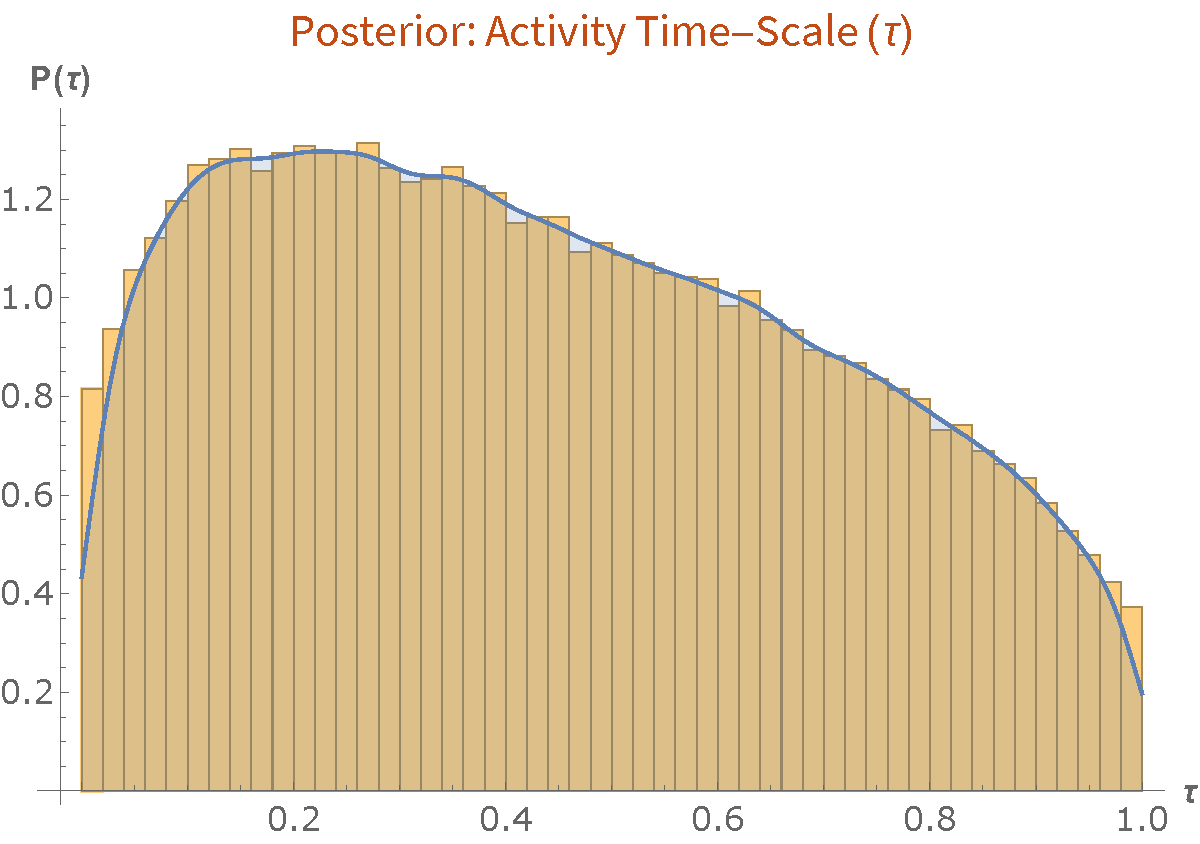
\includegraphics[width=\textwidth]{images/nft_activity/posterior_tau}
		\caption{}
	\end{subfigure}
	\begin{subfigure}{0.475\textwidth}
		\centering
		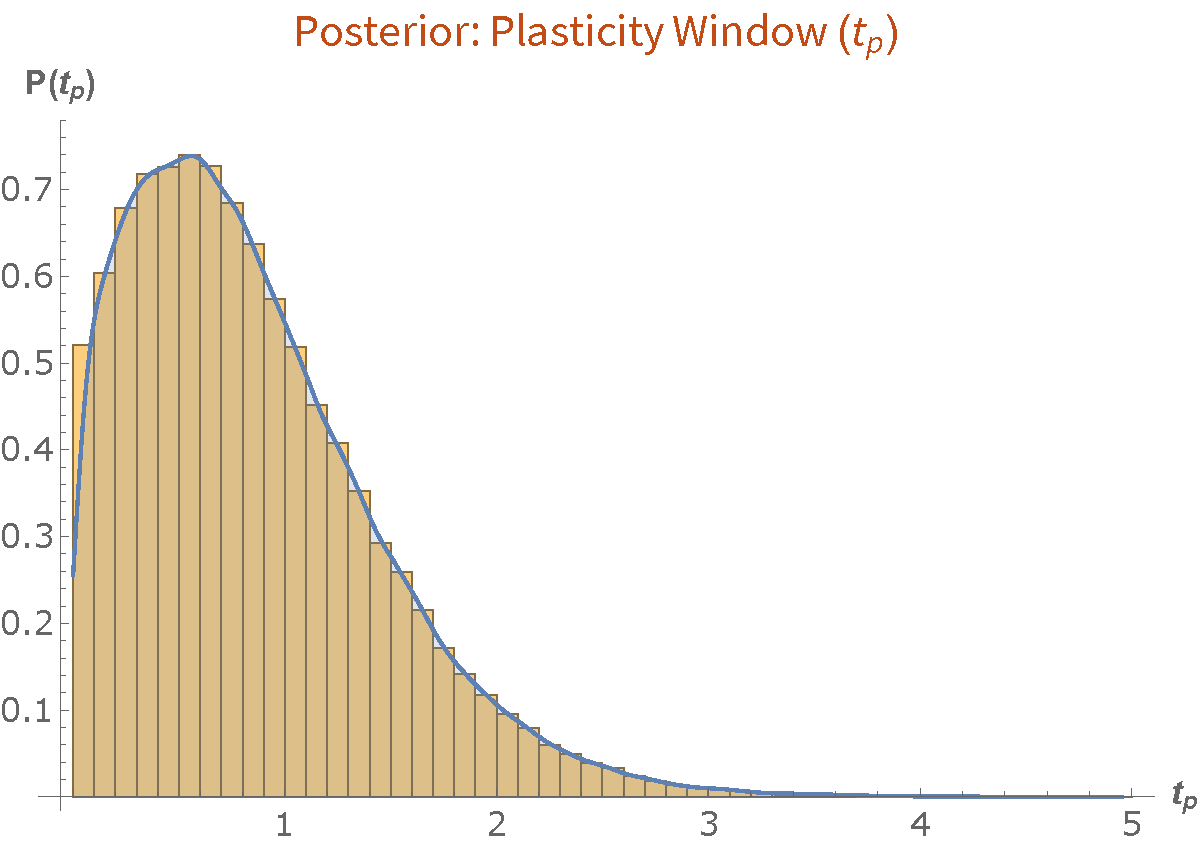
\includegraphics[width=\textwidth]{images/nft_activity/posterior_tp}
		\caption{}
	\end{subfigure}
	\begin{subfigure}{0.475\textwidth}
		\centering
		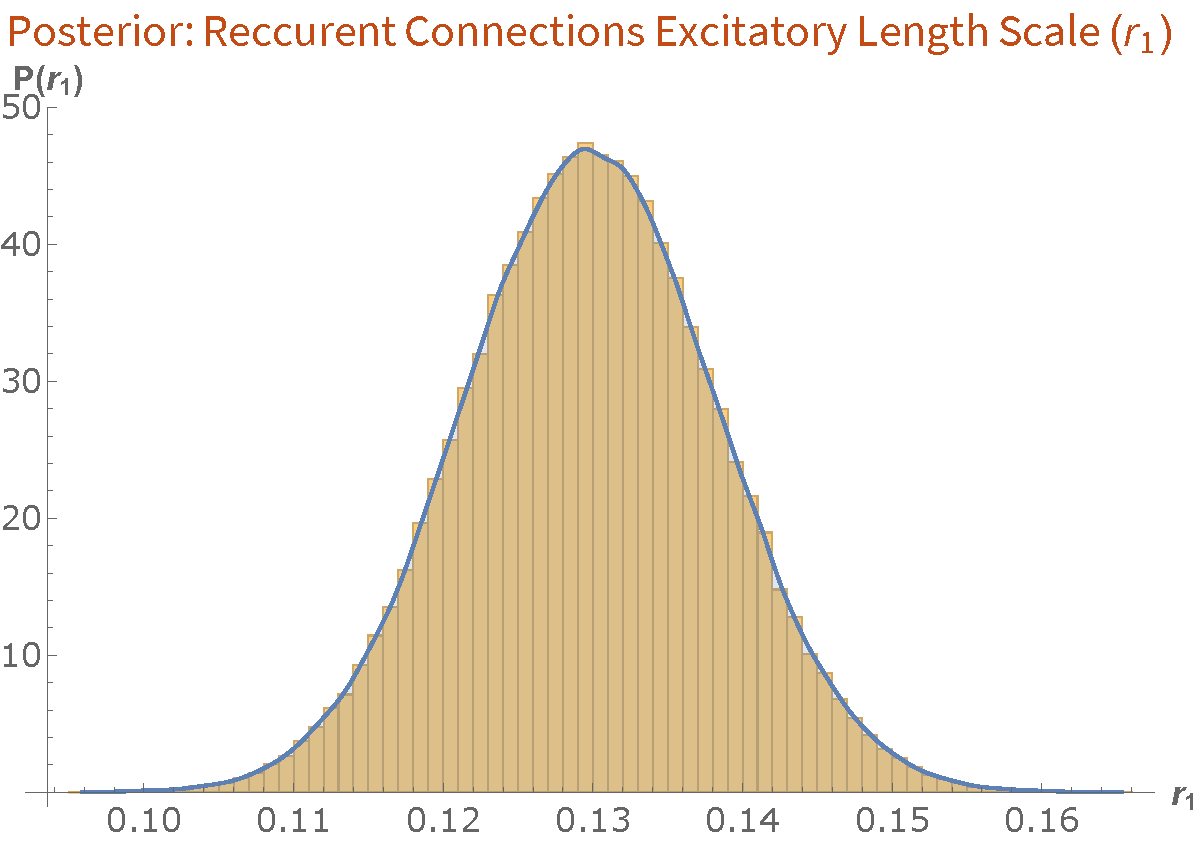
\includegraphics[width=\textwidth]{images/nft_activity/posterior_r1}
		\caption{}
	\end{subfigure}
	\begin{subfigure}{0.475\textwidth}
		\centering
		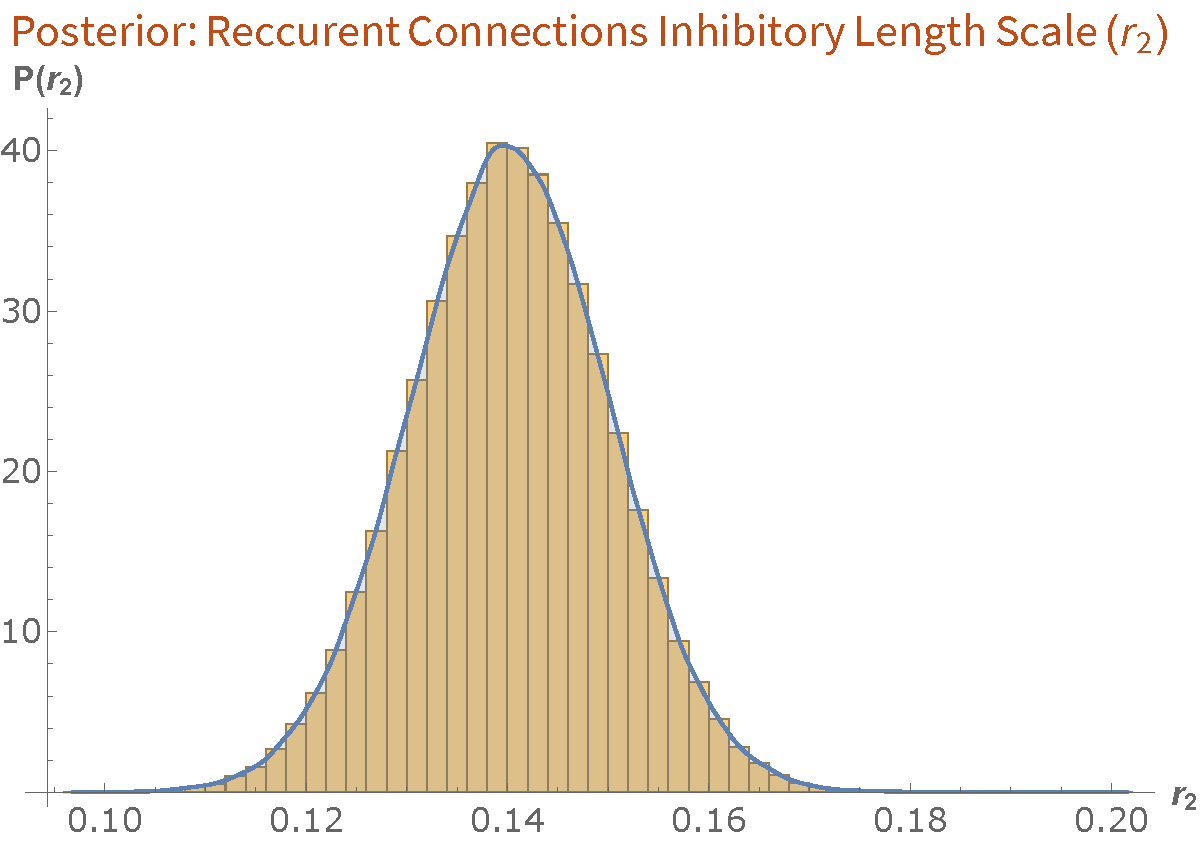
\includegraphics[width=\textwidth]{images/nft_activity/posterior_r2}
		\caption{}
	\end{subfigure}
	\begin{subfigure}{0.475\textwidth}
		\centering
		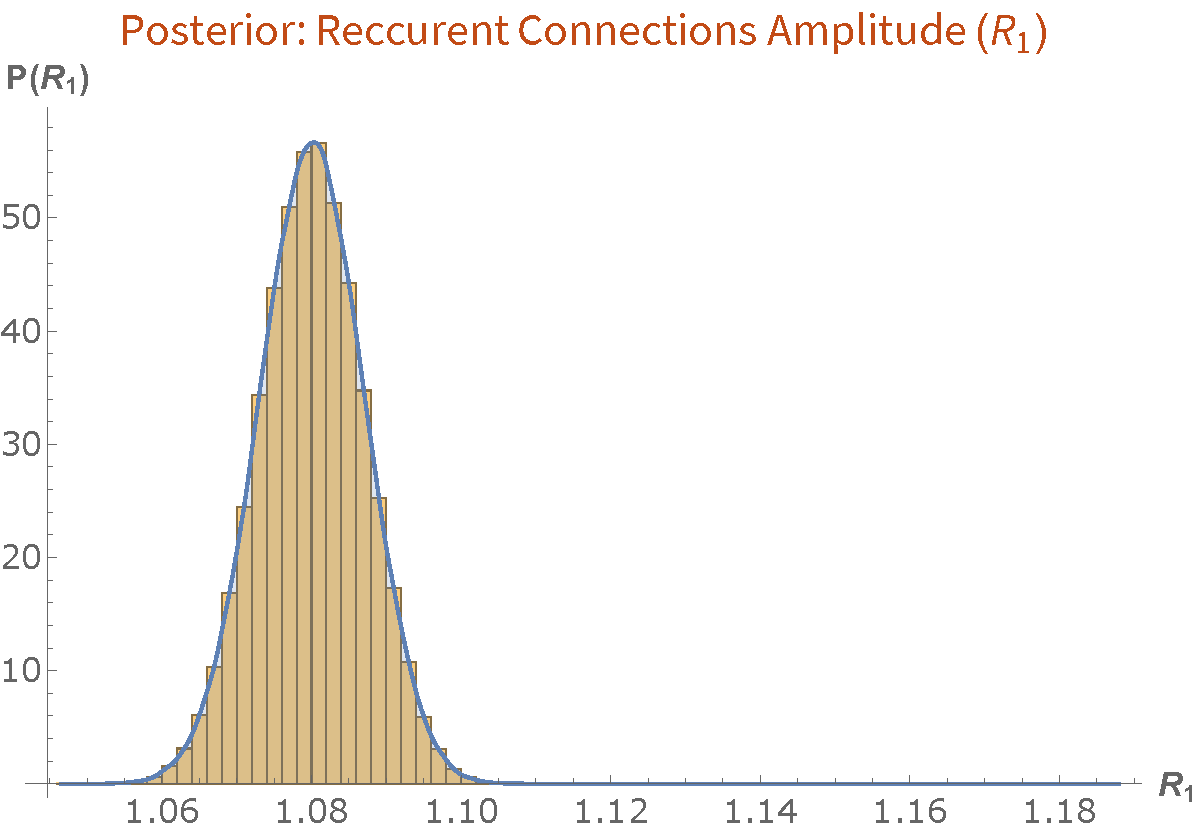
\includegraphics[width=\textwidth]{images/nft_activity/posterior_R1amp}
		\caption{}
	\end{subfigure}
	\def\c{The posteriors for the relevant model parameters after an MCMC regression. }
	\caption[\c]{\label{fig:posteriors} Panel (a) shows the posterior histogram for the time-scale of activity which is broadly distributed through the search space of [0,1]s but biased towards the lower bound. This broad distribution is concordant with the observation that the time-scale of activity induces relatively small variations in the organisation width; see Figure \ref{fig:parametereximinations}. Panel (b) shows the posterior histogram for the time scale of the plasticity window which is maximised around 0.6s. The posterior histograms for the recurrent connection parameters $(r1, r2, R1)$ are shown in Panels (c-e) and are tightly constrained by their informative priors suggesting that there is no predicted effect on these connections in the $\beta2^{-/-}$ mutant. For all histograms presented an empirical distribution curve was fitted and overlain in blue.}
\end{figure*}
The arborisation widths are estimated as $0.24 \pm 0.077 \text{mm}$ (wild-type) and $0.48 \pm 0.15 \text{mm}$ ($\beta2^{-/-}$) by taking half the square root of the arborisation area reported by Dhande et. al. (2011) \cite{Dhande2011-jp}. The wave speeds are estimated as $0.13 \pm 0.015 \text{mm s}^{-1}$ (wild-type) and $0.17 \pm  0.03 \text{mm s}^{-1}$ ($\beta2^{-/-}$), and the wave-widths as $0.11 \pm 0.012 \text{mm}$ (wild-type) and $0.20 \pm 0.012 \text{mm}$ ($\beta2^{-/-}$) by taking half the total width reported by Stafford et al (2009) \cite{Stafford2009}. The inhibitory and excitatory lengths scales, and amplitude of the recurrent connections are estimated as $0.14 \pm 0.014 \text{mm}$ and $0.13 \pm 0.013 \text{mm}$, and $1.08 \pm 0.01 \text{mm}$ respectively using the data reported by \cite{Phongphanphanee2014-in}. The priors on these parameters are taken as normal distributions centred on the estimates with standard deviation corresponding to the measurement error. Uninformative priors on the time-scale parameters are taken assigning uniform distributions on [0,1] and [0,10] for the activity time scale ($\tau$) and the plasticity window scale ($t_p$), respectively. The MCMC was completed using a dedicated Mathematica package \cite{Burkart2017}. The MCMC completed in $10^5$ iterations using 6 chains with each parameter initialised within 10\% of the mean of its prior. The maximum Gelman-Rubin statistic for convergence was $1.00037$ indicating that the chains had converged \cite{Gelman1992-pk}. The posteriors for each parameter are reported in Figure \ref{fig:posteriors}. The posteriors for the recurrent connections parameters, $r1, r2$, and $R_1$ remained tightly constrained by their priors, indicating that the prior estimates were well informed and in agreement with the model. The activity time scale is broadly distributed throughout the range [0,1]s with a bias towards 0. The plasticity time-scale is distributed around a maximum of $0.56$s. The computed $R^2$ statistic was 0.81. The code base for these simulations is freely available online \cite{NFT}.
\section{Discussion}
If the model is sound and the biological system is allowed sufficient time to reach a reasonable approximation of the asymptotic state then these results suggest that the computational/synaptic structures developed are primarily a result of activity dynamics. Under this model the chemotactic and competitive mechanisms serve to initialise a coarse isotropic retinotopy from which the activity dynamics can refine and ultimately dictate final synaptic organisation. This interpretation augments the understanding of the establishment of retinotopy by suggesting that the final synaptic organisation can be understood in a large part by understanding the spatio-temporal nature of the input stimulus, the recurrent connectivity, and the learning rule. Should the biological system not employ the learning routine until asymptotic stability then the model will still be able to make predictions about the final organisation given precise enough measurements of the relevant parameters. In both instances the model gives testable hypotheses the former of which has been benchmarked against the mouse wild-type and $\beta2^{-/-}$ mutant.

\paragraph{Organisation}
The key aspects of the final organisational structure are dictated by the interplay between the spatio-temporal characteristics of the input stimulus and the structure of the recurrent connections. These dependencies on recurrent connections and input are in accordance with previous analysis performed with a simple Hebbian rule and static input \cite{Takeuchi1979-zy}; the model proposed here, however, allows for richer construction in terms of specifying the input and connections by realising full temporal and spatial dynamics, and more complex structure in the final organisation. Regularisation rules were introduced which allow this organisation to take non-trivial structure when supplemented by system noise which is assumed able to be renormalised in downstream biological calculations or via some other mechanism. The regularisation necessitates neurotrophic factors being expressed during development. Finally, the measurable aspects of the organisation are dictated by the precise realisation of the relevant biological parameters.
\paragraph{Refinement}
The results indicate parameter dependence on wave-speed, wave-width, plasticity time-scales, and the ratio of excitation to inhibition widths in the recurrent connections. Principally, parameter changes that would lead to a tighter correlation structure such as smaller wave-widths, slower wave-speeds, and smaller excitatory zones lead to a smaller width of topographic refinement. Interestingly, the time-scale of the plasticity rule has an effect of the width of the final organisation. The $\beta2^{-/-}$ mutant provides a phenomenological test of this component of model. The knock-out exhibits fast-moving, and hyper-correlated, retinal waves which lead to an imprecise topographic mapping - an effect that has not been captured in existing models. The model suggests that an increase in wave-speed or wave width will lead to a less-refined map reproducing the results of the knock-out \textit{in silico}; see Figure \ref{fig:parametereximinations}. 

An MCMC parameter estimation was performed using known errors-in-measurement of wave-speed, wave-width, and organisation width in wild-type and the $\beta2^{-/-}$ mutant. The model predicts the expected mean width of both wild-type and the $\beta2^{-/-}$ mutant within standard error when parametrized by likelihood maximising parameters and provides a good explanation of the variance between the wild-type and mutant ($R^2$ = $0.81$).  The model is insensitive to the time-scale of activity with the posterior assuming a broad posterior over $[0,1]$s with a slight bias towards lower values suggesting that the activity time-scale does not account for much of the variance in organisation width. The posteriors of the parameters of the recurrent connections were largely dictated by their priors suggesting that the priors estimated from available are informative and that the $\beta2^{-/-}$ mutant does not have a substantial effect on the recurrent connections, as expected. The time-scale of the plasticity window is not expected to be affected by the knock-out and thus the MCMC allows us to estimate this parameter on the order of seconds. { The timescale of the plasticity window in two closely related biological systems, the Xenopus retinotectal projection and rat visual cortex, are estimated to be on the order of $10^{-2}$ seconds \cite{Froemke2002-be, Zhang2000-lb}. Plasticity windows can have significantly longer time-scales on the order of 10s of minutes \cite{Citri2008-kv}. The estimate is notably higher than what has been observed in similar systems but is in agreement with the typical duration of a wave of spontaneous activity in the developing retina in mice \cite{Xu2015-uc}. Deviation is expected in analysing a different biological system. This result suggests that the plasticity windows in this system are calibrated to integrate all information contained in a spontaneous wave event.}
\paragraph{Limitations}
The model presented here has several key limitations: dimensionality,  stimulus representation, simplicity of asymptotic solution, non-rigorous estimate of recurrent connectivity. The model is one dimensional while the surface of the superior colliculus is a two dimensional sheet. Two dimensional systems allow for a much richer topology and complicated dynamics which would be best examined numerically. The stimulus was assumed to be a simple wave-packet travelling left or right at a fixed speed and these directions were assumed to be equiprobable. These assumptions do not hold in two dimensional recordings with a directional bias being observed in retinal waves in mouse \cite{Ackman2012-uu}. The assumptions allowed an analytical solution to be derived which assisted with the MCMC simulations but is valid only asymptotically. The biological system has fixed developmental time frames and critical periods. Finally, the recurrent connections are assumed to be the difference of two Gaussian's with parameters estimated from a fit made to electrophysiological recordings \cite{Phongphanphanee2014-in}. This assumption is reasonable but would require extensive validation and a more rigorous biological underpinning would be desirable.
\paragraph{Future Directions}
The limitations listed above outline a clear direction for future study: extensive numerical simulation in a two dimensional context. The analysis can be trivially extended into the plane by using the same assumption: every wave-direction is equiprobable. A more realistic simulation can be conducted using data from a repository of retinal waves or by generating synthetic data from a wave-model \cite{Eglen2014-fo, Godfrey2009-rs}. A challenging aspect of this line is computational cost: the analytical solution is cheap to evaluate but numerics will take substantially longer. A method of mitigating this is by using GPU architectures and exploiting the parallelisation benefits of matrix multiplication which is required to evaluate the convolutional integrals. GPU parallelisation will be used in following chapters for similar reasons. This can be complemented with solvers developed for the Julia computing language which offer good numerical performance \cite{Sequeira2022}.

The model predicts that the time-scale of the plasticity window in developing mouse SC neurons is an order of magnitude higher than the scale typically used to describe neuronal plasticity in analogous systems. This prediction is not claimed to represent a ground truth, the model makes several simplifying assumptions and estimations, but it is a good candidate for experimental falsification.
\paragraph{Key Summary}

\begin{enumerate}
	\item \textit{An NFT modelling framework has been developed to allow for the incorporation of complex spatial statistics of retinal waves. Within this framework an analytical solution for plausible input stimulus was derived allowing for efficient computation.}
	\item \textit{Bayesian statistical regression showed the model can explain existing wild-type and mutant data. The regression also made a falsifiable experimental prediction about the time-scale of plasticity estimating it at ~0.5 a second in mice.}
	\item \textit{The model is naturally extendable to two dimensions and allows for efficient numerical simulation of realistic biological wave statistics.}
\end{enumerate}          
\chapter{Lattice Method Analysis: Analysing a Stochastic Development Hypothesis \label{chapter:lattice}}
\section{Preface}
\textit{The following chapter contains work from the paper \textbf{Detailed analysis of the double functional maps
in EphA3 knock-in mice} researched and written in collaboration with David Willshaw at the University of Edinburgh \cite{Willshaw2022-fs}. The research aim was to rigorously investigate the claim that the EphA3 heterozygote is on the border of a bifurcation point where it can phenotypically present itself in a stochastic manner as a wild-type, homozygote, or some mixed state in between, dependent on the neural activity patterns \cite{Owens2015-zv}. The biological data analysis using the lattice method was performed by primarily by David Willshaw and will be included in this chapter in Section \ref{section:davidsresults} to contextualise my theoretical results presented thereafter. The predominate focus of the chapter will be to recreate the experimental pipeline computationally and use modelling efforts to interrogate the central claim of stochasticity in the development of heterozygous mice. } 
\section{Introduction}
The individual effects of chemotaxis and neural activity have been discussed in both experimental and modelling contexts and subsequent theory has been developed for the individual contribution of these mechanisms: chemotaxis establishes a coarse topography on the basis of relative signalling while neural activity works to refine this interaction through a spatio-temporal patterning of spontaneous activity before eye-opening; see Section \ref{section:developmentaltheory} for a complete review and Chapter \ref{chapter:neuralstdp} for a detailed account of modelling activity in the wild-type and $\beta2^{-/-}$ genotype cases. The relative effects that these two developmental systems have on each other is less clearly understood with suggestions that activity patterns may regulate Eph/ephrin expression \cite{Lyngholm2019-fs, Nicol2007-rt}. A recent hypothesis is that chemotaxis and neural activity are finely balanced in the wild-type mouse but stochastic map generation can be achieved by manipulating chemical gradients and thus these mechanisms are ultimately stochastic in nature \cite{Owens2015-zv}. 

This hypothesis was developed by performing intrinsic optical imaging scans on the superior colliculus of several wild-type and mouse mutants: EphA3$^{+/-}$, and EphA3$^{+/+}$ knock-ins and combined EphA3$^{+/-}$$\beta2^{-/-}$. As discussed in Section \ref{sec:epha3} the EphA3 receptor is not endogenous to mouse and it is knocked in on the Islet2 expressing cells in the retina resulting in a boost of EphA receptor in a random salt-and-pepper distribution across the retina \cite{Brown2000-da, Reber2004-wq}. Retrograde DiI injections revealed that in the homozygous knock-in a complete duplicated map is formed: for every retinal injection site there are two termination sites in the superior colliculus along the rostrocaudal axis; see Figures \ref{fig:epha3anatomical} and \ref{fig:epha3collapse}. The heterozygotes follow a similar relationship but the duplicated projections are restricted to the caudal region of the colliculus collapsing into a single projection rostrally \cite{Brown2000-da}. These make it an excellent candidate to study perturbative effects in chemical signalling.

An intrinsic optical imaging scan is performed by stimulating a mouses visual field with a regular periodic signal and measuring the phase of the induced activity in the colliculus: the phase should correlate with the average retinal position of the signal along the stimulating axis; see Section \ref{sec:optical}. Optical imaging scans revealed that the homozygous knock-ins reliably produced a functional double map suggesting that the wild-type and EphA3$^{+/+}$ populations are segregated \cite{Cang2008-ez}. The technique was then performed on heterozygous knock-ins by Owens et. al. (2015) and revealed a highly variable phenotype: it would phenotypically present as a wild-type, a homozygote, and a class of mixed state in between; see Figure \ref{fig:owens}. To understand this variability in the context of activity they disrupted activity patterns by creating a EphA3$^{+/-}\beta2^{-/-}$ mutant and remarkably optical imaging experiments revealed that the variable heterozygous states collapsed into a wild-type phenotype. These results were corroborated with a computational model: the restricted competition Tsigankov-Koulakov model of unified mechanism \cite{Tsigankov2006-uy}. They showed this model can phenomenologically reproduce the EphA3$^{+/+}$ phenotype by adding additional EphA, here called $\Delta R$, in a subset of cells in the retina distributed in a salt-and-pepper fashions. They demonstrated that when this $\Delta R$ was tuned to a point in-between wild-type and homozygous levels the model qualitatively produced maps similar to those observed experimentally. These data were collectively interpreted by Owens et. al. (2015) in the following manner: there exists a fine balance between neural activity and chemotactic developmental mechanisms. The heterozygous knock-in exists on the border of a bifurcation point between the regular wild-type and homozygous mapping. At this bifurcation point the model suggests activity dependent mechanisms stochasticly cause the heterozygote present in a heterogeneous plethora of states. Investigation of this hypothesis of stochastic interaction between developmental mechanisms will be the primary focus of this chapter.
\begin{figure}[h!]
	\centering
	\includegraphics[width=\textwidth]{images/lattice/owenscomp}
	\def\c{The diversity of intrinsic optical imaging scans captured in the Owens et. al. (2015) dataset. }
	\caption[\c]{\c The experimental is shown in panels A-C. A representative set wild-type scans is shown in panels D and E. The scans for heterozygous EphA3 knock-in without altered neural activity patterns, EphA3$^{+/-}$$\beta2^{+/-}$, are presented in panels F and G. The EphA3$^{+/-}$$\beta2^{-/-}$ with disrupted neural activity patterns are presented in panels H and I. Representative scans of the  EphA3$^{+/-}$ heterozygote knock-in are shown in panels J-O and show phenotypes corresponding to wild-type, a mixed state, and EphA3$^{+/+}$ homozygotes. Representative EphA3$^{+/+}$ homozygote scans are shown in panels P and Q. Figure adapted from Owens et. al. (2015) \cite{Owens2015-zv}. \label{fig:owens}}
\end{figure}

\FloatBarrier
These data and observations provide several interesting challenges from a theoretical perspective with the principle question being: where is the stochasticity in the data arising from? The model is stochastic but the stochasticity is used as a minimisation technique and this does not necessarily imply stochasticity in the developmental mechanisms \cite{Tsigankov2006-uy}. Critically, the model enforces a one-to-one mapping between retinal and collicular locations which implicitly models the competitive nature of development but is arbitrarily strict and physically unrealistic. When combined with the Metropolis-Hastings methodology for energy minimisation this condition limits the search space of possible maps and can introduce artefacts not related to the underlying biology. This version of the model was later updated by Triplett et. al. (2011) to include a more realistic realisation of competition and is therefore a more appropriate theoretical tool with which to investigate this hypothesis --- this updated model was not discussed by Owens et. al. (2015) \cite{Triplett2011-jk, Owens2015-zv}. The stochastic nature of the data also provides an avenue to explore the underlying statistical properties of the model and methodologies to explore its parameter space which has not been historically done; see Section \ref{sec:koulakov}. 

The data analysis performed by Owens et. al. (2015) will be summarised followed by the reanalysis of the data done by David Willshaw which will contextualise the following modelling work \cite{Owens2015-zv}. A pipeline which is able to capture the intrinsic optical imaging process will be developed so that the recorded functional maps can be unified by with the underlying anatomy predicted by the model. This pipeline will allow the generation of lattice objects which can be compared with the biological data and also be used to generate distributions of relevant statistics to explore the principal hypothesis.
\section{Data Analysis \label{section:owensanalysis}}
The dataset generated by Owens et. al. (2015) is comprised of intrinsic optical imaging scans from 16 EphA3$^{+/-}$ mice, 5 homozygous EphA3$^{+/+}$ mice, and five wild-type mice \cite{Owens2015-zv}. The perturbations are restricted to the nasotemporal-rostrocaudal projection which varies primarily azimuthally and the original analysis accordingly generated 1-dimensional mapping profiles along this axis taken along three straight lines drawn through the colliculus which were thought to correspond with iso-elevational lines. For each of the three profiles the correlation coefficient was computed and two indexes were generated as functions of the three correlation coefficients: the linear fit index and intra-map index. These indexes were plotted against each other which revealed clustering of wild-type and homozygous specimens with the heterozygotes distributed between. There are two salient potential issues with this analysis: straight collicular lines do not correspond to iso-elevational contours and the clustering analysis indexes correlate with each other. The first issue may be resolved by realising that each of the image coordinates corresponds to a physical location which can be registered between the elevational and azimuthal scans and the elevational scan may be used to trace iso-elevational lines. The second issue may potentially not interfere with the end result but cannot be resolved.
\subsection{Reanalysis of Experimental Data \label{section:davidsresults}}
David Willshaw performed extensive reanalysis of the dataset in the context of our collaboration to complement the original analysis performed by Owens et. al. (2015) and will be summarised here. The analysis combined the elevational and azimuthal scans so that each collicular pixel had an associated coordinate in visual space thereby having a datum of the four dimensional topographic object discussed in Section \ref{sec:dimensionspace}. The colliculus region is defined by an ellipse encompassing the region where the stimulus excitation from the visual field is highest \cite{Kalatsky2003-cz}. The data then went through two filtering schemes to improve quality. First, the bulk, or average, activity was calculated for each pixel in the collicular region over the time course of the stimulation and the 10000 most active were selected. Second, the mean phase convolved over a pixel width of 5 was calculated and when the standard deviation of this mean is three times greater than the wild-type standard deviation the pixels are excluded. This step was performed because when the stimulus reaches the boundary of a functional map it will be stimulated from two distal retinal locations and thus be highly variable \cite{Willshaw2014-ms}. The phase measurement will be associated with the average position of these two distal locations and it cannot be reliably mapped to either; a problem associated with the subjectivity of the visual-collicular projective map discussed in Section \ref{section:receptivefield}. These filtering processes allow the definition of a complete map conditioned on the visual stimulus of physical collicular locations. The pixels that constitute these maps are represented in grey, and the pixels that are filtered in green. Three curves of iso-elevation are shown in the eligible grey pixels at $-25^\circ$, $0^\circ$, and $25^\circ$ which are represented in orange, cyan, and brown respectively.

With a complete representation of the topographic relationship the Lattice method of data analysis can be applied to each of these datasets discussed in Section \ref{sec:lattice}.A subset of eligible pixels with a mean spacing of 6 pixels was chosen or 80$\mu$m to tile the colliculus. The spacing between collicular nodes was chosen to be the smallest that gives highly ordered 2D maps in wild-types, as found in an analysis of another data set \cite{Willshaw2014-ms}. The mean visual field of all pixels falling with 3 pixels of these locations was calculated and associated with each location. The tiling was projected to the visual field and any edges found to be crossing were removed and highlighted in red with the resulting map giving a standardised topographic representation of the data: a lattice object. In the case of the heterozygotes and homozygotes and the data may be further subdivided into rostral and colliculus portions by creating a partitioning line through the excluded high variance points (green). This line was fitted by visual examination. Each of these regions can be associated with a part-map or lattice object constructed from pixels only in this region. An example of the lattice object generated for a wild-type is shown in Figure \ref{fig:wild-type1}. The variation in the iso-elevational lines indicates a marginal distortion in the dorsal-ventral axes.  

\begin{figure}
	\centering
	\includegraphics[width=\textwidth]{images/lattice/figwt}
	\def\c{An example of a lattice generated from a wild-type dataset. }
	\caption[\c]{\label{fig:wild-type1}\c The scale bar is 200um. There are several conventions in the image worth outlining. First, the green pixels are filtered data while the grey indicates the retained data. Second, the whole map is presented to the left conventionally while the largest ordered submap is presented to the right. The excluded links are highlighted in red in the original map and have a corresponding red cross on the submap. The three iso-elevational lines are represented in brown, cyan and orange. This example represents an excellent local ordering as only 4\% of the nodes had to be removed to give the largest ordered submap and high polarity scores. Figure reproduced from Willshaw and Gale (2022) \cite{Willshaw2022-fs}.}	
\end{figure}

For each dataset the lattice objects were to calculate a series of statistics and the following are chosen for this thesis: azimuthal and elevational magnification, map quality, and visual field overlap. Magnification ratio is a measure of the relative extent of the projection along a specified axis. The Azimuthal Magnification (AM) is the length of each edge measured along the rotated nasotemporal axis of visual field compared to the length of the corresponding edge along the rostrocaudal axis of the colliculus; similarly for the Elevational Magnification but this is of less interest in genotypes with disrupted A-system signalling.  Map quality refers to the number of nodes which need to be removed in order to form the perfect topographic representation. In cases when two maps were constructed by partitioning the colliculus, the extent of visual field which projects to both regions of the colliculus, called the Visual Field Overlap (VFO), was measured. In a complete double map, the VFO is the entire extent of visual field. These statistics were used to classify the heterozygotes into three categories concordant with the Owens et. al. analysis: HETA, HETB, and HETC. Example maps for these three heterozygote categories are shown in Figure \ref{fig:examples}.

The statistics associated with each population are shown in Table \ref{table:lattticestats}. The HETA classification shows very similar statistical profiles to the wild-type with no visual field overlap being recorded. The HETB specimens are beginning to deviate particularly in VFO. The HETC specimens present more similarly to HOM specimens with similar VFO and map qualities. The azimuthal magnification is distinguished between the two part maps due to the compression of each map into a region of the colliculus. The elevational magnification remains unchanged. The Lattice method has revealed evidence for two part maps in all of the homozygotes and to a lesser degree each of the heterozygotes. These part maps are formed by bisecting the colliculus into two regions on the basis of data quality and when this bisection is made each of the part maps form individual higher quality lattices than the whole map lattice. These higher quality maps can be used to interrogate the coverage of the visual field and in particular the overlap of the visual space covered by each part map: the VFO. 
\begin{table}[h!]
	\centering
	\begin{tabular}{|c|c c c c c|}
	\hline
	\textbf{Statistic}  & Wild Type & HETA & HETB & HETC & Hom\\
	\hline
	Whole Map AM & $1.54  \pm -$ & $0.93 \pm 0.13$ & $1.03 \pm 0.11$  & $1.11 \pm 0.12$ & $1.49 \pm 0.2$ \\
	Rostral AM & $- \pm -$ & $0.26 \pm 0.36$ & $1.16 \pm 0.1$  & $1.34 \pm 1.34$ & $2.03 \pm 0.2$ \\
	Caudal AM & $- \pm -$ & $0.41 \pm 0.57$ & $0.81 \pm 0.07$  & $ 0.75 \pm 0.75$ & $1.03 \pm 0.27$ \\
	Whole Map Quality & $91 \pm 4$ & $86 \pm 2$ & $91 \pm 5$  & $78 \pm 19$ & $71 \pm 10$ \\
	Rostral Quality & $- \pm -$ & $- \pm -$ & $97 \pm 1$  & $93 \pm 6$ & $91 \pm 6$ \\
	Caudal Quality & $- \pm -$ & $- \pm -$ & $88 \pm 9$  & $89 \pm 8$ & $90 \pm 15$ \\
	VFO& $- \pm -$ & $0 \pm 0$ & $5 \pm 2$  & $ 27 \pm 13$ & $33 \pm 18$ \\
	\hline
	\end{tabular}
	\def\c{Summary statistics based on the lattice analysis. }
	\caption[\c]{\c The magnification ratios for each of the part maps are summarised (where appropriate) with the rostral projection and the caudal projection is reported in parenthesis and square brackets respectively. The whole map quality is shown to degrade from wild-type to homozygote and the average part map quality is reported in parenthesis and square brackets respectively. The VFO increases from wild-type to homozygotes. The VFO and map quality statistics appear to be the most relevant statistics to query whether there is a significant overlap between classifications. These statistics are generated on small samples (~5 specimens each) and caution should be applied interpreting them. \label{table:lattticestats}}
\end{table}
\begin{landscape}
\begin{figure}[h!]
	\centering
	\begin{subfigure}{0.75\textwidth}
		\centering
		\includegraphics[width=\textwidth]{images/lattice/figHETA1}
		\caption{\textbf{HETA}}
	\end{subfigure}
	~
	\begin{subfigure}{0.75\textwidth}
		\centering
		\includegraphics[width=\textwidth]{images/lattice/figHETB1}
		\caption{\textbf{HETB}}
	\end{subfigure}
	
	\begin{subfigure}{0.75\textwidth}
		\centering
		\includegraphics[width=\textwidth]{images/lattice/figHETC2}
		\caption{\textbf{HETC}}
	\end{subfigure}
	~
	\begin{subfigure}{0.75\textwidth}
		\centering
		\includegraphics[width=\textwidth]{images/lattice/figHOM2}
		\caption{\textbf{HOM}}
	\end{subfigure}
\end{figure}
\end{landscape}
\addtocounter{figure}{-1}
\begin{figure}[h!]
\def\c{Examples for the three heterozygous classifications and the homozygous maps. }
\caption[\c]{ \c For each of these maps the whole map lattice is calculated and shown in the left and the rostral and caudal part-maps are shown on the right; the scale bar is 200um.. An example map for the A classification is shown in panel (a) and shows a very small secondary part map with reversed polarity. When the two part-maps are disambiguated the map quality improves with less nodes being removed compared to the whole map and the first part map corresponds well to a wild-type. An example map for the B classification is shown in panel (b) and while the whole map suggests a degree of ordering it is improved by separating the projection at the neck of the eligible pixels in grey. An example map for the C classification is shown in (c) and here map quality is substantially improved by segregation with a complete visual representation rostrally and a partial visual representation caudally; these heterozygotes are qualitatively similar to homozygotes in this respect. An example map of a homozygote is shown in (d) with the eligible pixels completely forming two independent regions and with each of these regions containing a well ordered and substantial portion of the visual field. Figure reproduced from Willshaw and Gale (2022) \cite{Willshaw2022-fs}. \label{fig:examples}}
\end{figure}
\section{Modelling Pipeline}
To theoretically analyse the stochastic hypothesis there needs to be a method to directly compare model output with data elements. There are two key issues here: registration and anatomical interpretation. The lattice method provides a good solution to the first problem as it is defined topologically and therefore lattice properties such as visual field coverage can be compared between two model runs without needing to ensure that all points are metrically registered against each other. The method also allows for direct comparison to the data under the hypothesis that the model generates comparable data-types. This leads to the second problem which is how the Tsigankov-Koulakov connections are precisely defined. The most reasonable interpretation given the data used to define the models is that they are anatomical, not functional \cite{Tsigankov2006-uy, Koulakov2004-ia, Tsigankov2010-on, Triplett2011-jk}. For the wild-type phenotype the distinction is irrelevant because the functional imaging scans would be in correspondence with the anatomical retinotopy. However, when there is a duplicated or ectopic connection this association is non-trivial. The phase of the signal will be now composed of several components of the visual field and the measured phases is the average phase of these components.

To compare the model and data the model is used as a network generator on which activity dynamics can be explored. The activity induced by the optical imaging paradigm can then be simulated and used to generate lattice objects which are comparable to data. This interpretation confers an additional benefit: the underlying anatomical properties of the network are completely known. Therefore anatomical lattices can be generated to make predictions about the underlying structure of maps. This is of particular interest in a related hypothesis: do the wild-type and EphA3$^{+/+}$ afferents completely segregate in the colliculus? A review by Cang and Feldheim (2013) implies that they do but this appears to be based on functional optical imaging scans while anatomical injection studies are too sparse \cite{Cang2013-dw}. These questions are intimately related to the role of competition with respect to gradient sensing mechanisms and therefore the choice of model is the Tsigankov-Koulakov model extended to have multiple connections and a competitive sorting mechanism \cite{Triplett2011-jk}. 

The anatomical model can be used as a blueprint retinotopic map on which to simulate neural activity which can be used to generate \textit{in silico} optical imaging scans. The lattice method can be used to generate statistics on this distribution of scans and thus directly compare with experimental data. The statistics of most interest for examining the heterozygote variability hypothesis are the VFO and map quality.  These two statistics can be used to classify the heterozygous variability under the following criteria: the part-map subdivision must not substantially improve map quality over the whole map to be classified as similar to wild-type and the VFO must be statistically similar to the homozygous distribution to be classified as a homozygote. 
\subsection{Anatomical Model}
The Tsigankov-Koulakov model shall be briefly covered here and it is detailed in full in Section \ref{sec:models}. The model is an energy minimization model which assigns energy to a configuration of synaptic connections between a set of collicular and retinal cells. The energy is given by:
\begin{align}
&E = E_{\text{chem}} + E_{\text{act}}+E_{\text{comp}}\\	
&E_{\text{chem}} = \sum_{p \in \{\alpha,\beta\}}\sum_{i \in \text{syn}} pR(i_\text{ret},p)L(i_\text{col},p) \\
&E_{\text{act}} =- \frac{\gamma}{2} \sum_{i \in \text{syn}}\sum_{j \in \text{syn}} C(d_R(i, j))U(d_C(i, j)) \label{eq:latticemodelequation}\\
&E_{\text{comp}} = \sum_{i\in \text{ret}} (n_i^2 - 500 n_i^{1/2}) + \sum_{i\in \text{col}} n_i^2.
\end{align}
The chemotactic term is given with $\alpha=-90$ $\beta=120$ with the change in sign indicating that the B system is attractive and the A system repulsive, $R$ and $L$ are the masked gradients (the difference between Eph and ephrin levels) in retina and SC locations respectively, and the sum is performed over all possible synapses; the parameters and gradients are inherited from previous iterations of the model. It is important to note that this masking ensures that the system is a Type I or graded matching. The activity term is the sum over all pairs of synapses of the product of two correlation functions which take the normed distance between a synapse pair in the retina, $C(d_R) = \exp(-|d_R|/11)$, and colliculus, $U(d_C) = \exp(-d_C^2/18)$, where the $d_R$ and $d_C$ are the metric functions for the retina and colliculus respectively and the parameters $11$ and $18$ and $\gamma=0.00625$. Finally, the competition term is given by two sums: one over over the SC and retinal locations. The sums compute the square of the number of synapses for the SC sites, and the difference between square and square root of the number of synapses for the retinal sites. In this fashion, it is energetically favourable to have some, but not too many, synapses between locations. The forms and parameters of the function are chosen arbitrarily.

The minimisation procedure involves the creation and deletion of synapses. At each simulation time-step a potential pairing of an SC and retinal site is considered and the change to the energy function that adding this site would induce is calculated. A uniform random number $u$ is generated and compared to:
\begin{equation}
p = \frac{1}{1+\exp(-4\Delta E)},
\end{equation}
and the change is accepted if $p<u$ thus promoting changes which lower the energy whilst stochastically accepting higher energies infrequently. The same procedure is repeated except sampling amongst existing synapses and preferentially deleting synapses which contribute high energy. The model was allowed to run for $5\times N^2$ time-steps where N is the number of cells in the colliculus and retina. The parameter choices made here follow the paper and Git repository for Hjorth (2015) \cite{Hjorth2015-le}. These parameters have produced good results in this study but it is still prudent to exercise caution about them given that there are no comprehensive studies exploring the parameter space of this model.

For high resolution maps the number of cells was chosen to be $N = 10000$ (in line with the number of active pixels in the data analysis) while for low resolution maps which converged quickly the number of cells was $N = 2000$. The model was implemented computationally using the MATLAB package developed by Hjorth et. al. (2015) \cite{Hjorth2015-le} on am AMD Ryzen Threadripper 3950X with 32 cores.

To model the EphA3 systems a fraction of retinal cells were chosen to be tagged as EphA3$^{+/-}$ cells. This fraction was typically 50\% but fractions of 40\% and 50\% were also examined. To each of these tagged cells an additional $\Delta R$ was added to their EphA level given by their position `$x$' in the EphA gradient $R_A(x)$. The gradients are normalised to a maximum value of one in the wild-type and it remains an open question what $\Delta R$ should be equal to. It seems reasonable that the homozygote should be twice that of the heterozygote but this does not follow automatically. In light of these considerations, a parameter sweep of $\Delta R$ was performed to understand its effects in parameter space more generally. The codebase used to perform the following simulations is freely available online \cite{LatticeEphA3}.
\newpage
\subsection{Spiking Model of Neural Activity}
To simulate activity in the superior colliculus a simple Poisson integrate-and-fire model was chosen; see Section \ref{sec:activity}. It was assumed that each collicular $i$ cell is connected to each retinal cell $j$ with a weight $W_R(i,j)$ given by the output of the anatomical model, and to other collicular cells $k$ with a weight given by the function of the distance $d_{ik}$ between them:
\begin{equation}
W_C(i, k) = w_1 \exp\left(-\frac{d_{ik}^2}{2r_1^2}\right) -w_2 \exp\left(-\frac{d_{ik}^2}{2r_2^2}\right),
\end{equation}
where the colliculus length was normalised to one and $r_1 = 0.01, r_2 = 0.02, w_1 = 0.02$, and $w_2 = 0.01$ to mimic the lateral connectivity pattern reported in the colliculus \cite{Phongphanphanee2014-in}. These are first order approximations of the recurrent kernel which differ from the estimates given in Chapter \ref{chapter:neuralstdp}. This is due to the slightly different geometries employed in each model. Each collicular cell receives input in the form of spikes from retinal cells and other collicular cells and these spikes are integrated over time to form the rate parameter:
\begin{equation}
r_i(t, t_0) = \int_{t0}^t dt \left( \frac{1}{\sum_jW_R(i,j)}\sum_{j} W_R(i,j) I_R(j, t) + \frac{1}{\sum_kW_C(i,j)}\sum_{k} W_C(i,j) I_C(k, t) \right),
\end{equation} 
where $t_0$ is the time of the last collicular spike in collicular cell $i$, and $I_R(j,t)$ and $I_C(k, t)$ are the spike trains for retinal index $j$ and collicular index $k$ respectively. The sampling rate was set at $dt = 0.01$ seconds and at each timestep $dt$ a random number $p_i$ was drawn and a spike generated in collicular index $i$ if:
\begin{equation}
r_i(t, t_0) dt < p_i.
\end{equation}
A record of all collicular spikes was generated and associated with collicular activity generated by stimulating the retina with a given input pattern, $I_R(j, t)$, chosen to represent the experimental paradigm described in Section \ref{section:OIS}. 
\newpage
\subsection{Optical Image Scan Reconstruction \label{section:OIS}} 
To reconstruct the optical images the procedure outlined by Kalastky and Strkyer (2003) was replicated \cite{Kalatsky2003-cz}. A wave of stimulus was applied across the retina as input in an orthogonal direction repeated with periodic boundary conditions ten times. The activity is propagated into the network model as a series of neuronal spikes generated by a Poisson process and this combined with lateral connectivity generates a series of spikes in the colliculus. The procedure is reversed and two records of the activity in the forward and reverse directions are kept. The entire procedure is again repeated along the complementary orthogonal direction and these are associated with azimuthal and elevational activity. Figure \ref{fig:activitydem} shows the phase plots for a wild-type phenotype, Figure \ref{fig:scans} shows the azimuthal phase plots for heterozygous and homozygous knock-ins. The lattice method can be applied directly to this surrogate phase data and forward (visual field to colliculus) and reverse (colliculus to visual) field are shown conventionally in blue and black respectively; see Figure \ref{fig:wholemap}.
\begin{figure}[h]
	\begin{subfigure}{0.5\textwidth}
		\centering
		\includegraphics[width=\textwidth]{images/lattice/WT1}
		\caption{}
	\end{subfigure}
	\begin{subfigure}{0.5\textwidth}
		\centering
		\includegraphics[width=\textwidth]{images/lattice/WT2}
		\caption{}
	\end{subfigure}
	\def\c{The azimuthal and elevational phase diagrams for a wild-type simulation. }
	\caption[\c]{The azimuthal and elevational phase diagrams for a wild-type simulation are presented in panels (a) and (b) respectively following the procedure outlined Kalatsky and Stryker (2003) \cite{Kalatsky2003-cz}. There is a good correspondence between these phases maps and those measured biologically. It is important to note that biological phase maps are stimulated azimuthally and conventionally and these roughly correspond with the orthogonal gradients in the retina but not precisely, in these maps this relationship is precise but the naming convention is kept.} \label{fig:activitydem}
\end{figure}
\FloatBarrier
	
\begin{figure}[h]
~\unskip\ \vrule\ 
~\unskip\ \hrule width0.985\textwidth
~\unskip\ \vrule\ 
	\begin{subfigure}{0.47\textwidth}
		\caption{Colliculus to Field: Whole Map}
		\centering
		\includegraphics[width=0.95\textwidth]{images/lattice/example_lattice_CTOF_whole}
	\end{subfigure}
~\unskip\ \vrule\ 
	\begin{subfigure}{0.47\textwidth}
		\caption{Colliculus to Field: Part Maps}
		\centering
		\includegraphics[width=0.95\textwidth]{images/lattice/example_lattice_CTOF_sub}
	\end{subfigure}
~\unskip\ \vrule\ 
~\unskip\ \hrule width0.985\textwidth
~\unskip\ \vrule\ 
	\begin{subfigure}{0.47\textwidth}
		\caption{Field to Colliculus: Whole Map}
		\centering
		\includegraphics[width=0.95\textwidth]{images/lattice/example_lattice_FTOC_whole}
	\end{subfigure}
~\unskip\ \vrule\ 
	\begin{subfigure}{0.47\textwidth}
		\caption{Field to Colliculus: Part Maps}
		\centering
		\includegraphics[width=0.95\textwidth]{images/lattice/example_lattice_FTOC_sub}
	\end{subfigure}
~\unskip\ \vrule\ 
~\unskip\ \hrule width0.985\textwidth
~\unskip\ \vrule\ 
	\def\c{A series of whole maps and part-maps generated on anatomical data for a simulation ($\Delta R = 0.565$). }
	\caption[\c]{\c Each panel has four lattices with the top two corresponding to retinal nodes and the bottom to corresponding to collicular nodes. The black lattices in panel A are constructed using the colliculus as the pre-image and represent the lattice object generated on the entire set of collicular nodes. The whole map lattice is presented on the left of panel A and the largest submap on the right with excluded links highlighted in red. The black lattices in panel B are the largest submap lattices constructed on the rostral and caudal nodes in the colliculus. To construct each of these submaps a partitioning line is created at the average rostrocaudal location of the filtered (green) nodes and the rostral partmap is constructed using collicular points left of this line and the rostral partmap using the points right of the line. The blue lattices in panel C are the whole map lattices as in Panel A but constructed using the retina as the pre-image in the Lattice Method. The lattices in panel D are part map lattices that are constructed using the $Islet2$ expressing cells (left partmap) and $Islet2$ non-expressing cells (right partmap); since both populations are relatively uniformly expressed on the retina the pre-image lattice has good retinal coverage which differs to the pre-image coverage of the collicular partmaps in B. Each of the partmap projections have an overlap which is highlighted in purple; this overlap for a collicular pre-image (black) corresponds to the VFO. This example highlights how carefully partitioning the colliculus (or retina) carefully can reveal well ordered properties that would not be measurable by analysing the map as a whole. \label{fig:wholemap}}
\end{figure}
\FloatBarrier
\section{Results}
The value of $\Delta R$ to generate a heterozygous or homozygous genotype is not known \textit{a priori} and therefore a range of values $\Delta R = \{0.0565 i\}_{i=0}^{i=10}$ was interrogated; this is analogous to assuming a uniform prior on the $\Delta R$ parameter. Several anatomical experiments are performed on these maps, followed by a lattice analysis, before attempting to analyse the statistical properties of these maps at a lower but more computationally manageable resolution.
\subsection{Anatomical Experiments}
The model allows the provenance of a synaptic connection to be recorded: a synapse's origin can be labelled as an EphA3 expressing or wild-type cell in the retina. In the following experiments this is exploited by labelling wild-type cells in red and EphA3 tagged cells in gold. 

Anterograde dye injections into the retina are made to stain the colliculus. From these the average projection location in the rostrocaudal of all cells within a given tolerance of 1\% in the nasal-temporal axis is calculated. The analogous retrograde injection into the colliculus to stain the retina is also performed. These simulations reproduce in a single map the experimental injections performed and averaged over many mice \cite{Brown2000-da}. The results are in accordance with those experiments demonstrating that the model predicts individual map presentations correlate closely with aggregate population maps. These experiments can be seen in the third and fourth rows of Figure \ref{fig:antomicalEphA3}.

Next, the whole retina was flooded with red and gold labelled dyes in an experiment analogous to the one performed for the $Math5^{-/-}$ mutant \cite{Triplett2011-jk}. This experiment reveals the area of the colliculus which each cell type is restricted to and is useful to provide a register for the domains of each cell type. For low amounts of $\Delta R$ the populations are fairly well mixed across the colliculus and become increasingly segregated with an increasing level of $\Delta R$. For the maximum observed level of $\Delta R=0.56$ the maps become completely almost completely segregated with a slight overlap. These experiments can be seen in the final row of Figure \ref{fig:antomicalEphA3}.
\begin{landscape}
\begin{figure}
	\centering
	\includegraphics[width=1.6\textwidth]{images/lattice/paper_anatomy_dr}
	\def\c{A series of injection experiments are performed on knock-in simulations with $\Delta R$ increasing left to right from $\Delta R=0$ (wild-type) to $\Delta R=0.565$ (HOM). }
	\caption[\c]{\c In each plot the EphA3 projection and cell-type is labelled in gold while the wild-type cell-type is labelled in red. The first row represents the average projection from collicular cells in the rostrocaudal axes to the nasal-temporal axes (colliculus-to-field), the second represents the average projection of the retinal cells into the rostrocaudal axis (field-to-colliculus), and the third represents the retinal providence of each collicular cell. In the colliculus a number of points are highlighted in blue and these correspond to an injection made of 1\% of the retina in the central field corresponding to the experiments performed by Brown et. al. (2000) \cite{Brown2000-da}.} \label{fig:antomicalEphA3}
\end{figure}
\end{landscape}
\subsection{Lattice Analysis}
The anatomical map for each sample of $\Delta R$ was used to perform an optical imaging experiment and example azimuthal scans are presented in Figure \ref{fig:scans}. After performing the same data filtering procedure used on the biological specimens a number of different lattice objects were generated on both the anatomical and functional maps. The lattices in both directions between visual field/retina and colliculus were generated. The the average rostrocaudal location of the filtered data was used to generate a discriminator to separate the two functional colliculus maps. The collicular cells in these regions where then used to generate a lattice onto the retina to give an indication of the quality of each of the functional maps. An analogous experiment in the retina was also performed whereby the mapping was restricted to a single cell type and another scan performed to generate the lattice that this cell restricted retina would have in the absence of interactions the other cell-type; the additional scan is necessary to remove these interactions.
\begin{figure}[h]
	\begin{subfigure}{0.45\textwidth}
		\centering
		\includegraphics[width=\textwidth]{images/lattice/hetA_DR08}
		\caption{\textbf{HETA: $\Delta R =  0.226$}}
	\end{subfigure}
~
	\begin{subfigure}{0.45\textwidth}
		\centering
		\includegraphics[width=\textwidth]{images/lattice/HetB_DR_10}
		\caption{\textbf{HETB: $\Delta R =  0.282$}}
	\end{subfigure}

	\begin{subfigure}{0.45\textwidth}
	\centering
	\includegraphics[width=\textwidth]{images/lattice/hetB_DR_12}
	\caption{\textbf{HETC: $\Delta R =  0.339$}}
	\end{subfigure}
~
	\begin{subfigure}{0.45\textwidth}
		\centering
		\includegraphics[width=\textwidth]{images/lattice/hom}
		\caption{\textbf{HOM: $\Delta R =  0.565$}}
	\end{subfigure}
	\def\c{The azimuthal phase diagrams for several heterozygote simulations and a homozygote simulation. }
	\caption[\c]{\c Panel (a) resembles a HETA type classification, Panel (b) resembles a HETB type classification, Panel (c) resembles a HETC type classification, and Panel (d) resembles a HOM classification. This demonstrates that under choices which correspond to experimentally observed knock-in values the optical imaging procedure can qualitatively reproduce the properties of the functional imaging data in biological specimens \cite{Reber2004-wq, Owens2015-zv}.} \label{fig:scans} 
\end{figure}
\FloatBarrier
\newpage
\paragraph{Whole Maps and Part Maps}
The differences between whole maps and part-maps are highlighted in Figure \ref{fig:wholemap}. The maps are constructed as projections from colliculus (black) and to colliculus (blue). The removed links in red when constructing the whole map are pervasive and indicate a lower quality map. By subdividing the region into two sections in the colliculus-to-field projection, or by conditioning on the cell type provenance in the field-to-colliculus projection the resulting part-map have a much higher quality. This subdivision is made automatically by finding the average rostrocaudal position of the cells that are filtered out in the data preprocessing stage; these filtered cells have a high variability in phase and likely indicate the boundary of the two populations. In the HET type simulation this provides evidence for two projections and this technique is used to analyse the effect of varying EphA3 in creating a detectable secondary projection.


\paragraph{Lattice Analysis of Varying EphA3 magnitude}
Two series of lattices, both derived from stimulating the colliculus and then using the associated phase-visual field link proposed by Kalatsky and Stryker (2003) to construct the lattice, were generated: the first selects points from the colliculus and projects into the field, the second projects from the field into the colliculus. To examine the evidence for a second projection appearing with increasing $\Delta R$ part-map lattices are constructed. These lattices are constructed in both directions and after filtering are shown in Figure \ref{fig:partmapsCTOF}. In each lattice the projection overlap is presented in purple. 
\begin{figure}
	\def\c{The colliculus-to-field part maps are shown in order of increasing $\Delta R$. }
	\caption[\c]{ Image on the following page. The colliculus-to-field part maps are shown in order of increasing $\Delta R$: the top row increases $\Delta R$ from wild-type levels up to HET levels, while the bottom row increases up to HOM levels. These levels are calibrated against the relative differences in measured mRNA expression levels for wild-type and EphA3 mice \cite{Reber2004-wq}. The noise introduced by the optical imaging procedure in the region of intermingling maps increases with $\Delta R$ mimicking biological observations. Both the rostral and caudal regions from a progressively larger cover of the visual field but the rostral region is of slightly lower quality. This is likely due to the compression of the EphA3 projection into the rostral region of the colliculus. \label{fig:partmapsCTOF}}
\end{figure}
\begin{landscape}
\begin{figure}[h!]
\hrule width1.505\textwidth
~\unskip\ \vrule\ 
\begin{subfigure}{0.475\textwidth}
	\caption{\textbf{WT: $\Delta R =  0.0$}}
	\includegraphics[width=\textwidth]{images/lattice/lattice_CTOF_0}
\end{subfigure}
~\unskip\ \vrule\ 
\begin{subfigure}{0.475\textwidth}
	\caption{\textbf{$\Delta R =  0.113$}}
	\includegraphics[width=\textwidth]{images/lattice/lattice_CTOF_04}

\end{subfigure}
~\unskip\ \vrule\ 
\begin{subfigure}{0.475\textwidth}
	\caption{\textbf{HET: $\Delta R =  0.226$}}
	\includegraphics[width=\textwidth]{images/lattice/lattice_CTOF_08}
\end{subfigure}
~\unskip\ \vrule\ 

~\unskip\ \vrule\ 
\begin{subfigure}{0.475\textwidth}
		\caption{\textbf{HET: $\Delta R =  0.339$}}
	\includegraphics[width=\textwidth]{images/lattice/lattice_CTOF_12}

\end{subfigure}
~\unskip\ \vrule\ 
\begin{subfigure}{0.475\textwidth}
		\caption{\textbf{$\Delta R =  0.452$}}
	\includegraphics[width=\textwidth]{images/lattice/lattice_CTOF_16}

\end{subfigure}
~\unskip\ \vrule\ 
\begin{subfigure}{0.475\textwidth}
		\caption{\textbf{HOM: $\Delta R =  0.565$}}
	\includegraphics[width=\textwidth]{images/lattice/lattice_CTOF_20}

\end{subfigure}
~\unskip\ \vrule\ 
\hrule width1.505\textwidth
\end{figure}

\begin{figure}[h!]
	\hrule width1.505\textwidth
	~\unskip\ \vrule\ 
	\begin{subfigure}{0.475\textwidth}
		\caption{\textbf{WT: $\Delta R =  0.0$}}
		\includegraphics[width=\textwidth]{images/lattice/lattice_FTOC_0}
	\end{subfigure}
	~\unskip\ \vrule\ 
	\begin{subfigure}{0.475\textwidth}
		\caption{\textbf{$\Delta R =  0.113$}}
		\includegraphics[width=\textwidth]{images/lattice/lattice_FTOC_04}
		
	\end{subfigure}
	~\unskip\ \vrule\ 
	\begin{subfigure}{0.475\textwidth}
		\caption{HET: $\Delta R =  0.226$}
		\includegraphics[width=\textwidth]{images/lattice/lattice_FTOC_08}
	\end{subfigure}
	~\unskip\ \vrule\ 
	
	~\unskip\ \vrule\ 
	\begin{subfigure}{0.475\textwidth}
		\caption{\textbf{HET: $\Delta R =  0.339$}}
		\includegraphics[width=\textwidth]{images/lattice/lattice_FTOC_12}
		
	\end{subfigure}
	~\unskip\ \vrule\ 
	\begin{subfigure}{0.475\textwidth}
		\caption{\textbf{$\Delta R =  0.452$}}
		\includegraphics[width=\textwidth]{images/lattice/lattice_FTOC_16}
		
	\end{subfigure}
	~\unskip\ \vrule\ 
	\begin{subfigure}{0.475\textwidth}
		\caption{\textbf{HOM: $\Delta R =  0.565$}}
		\includegraphics[width=\textwidth]{images/lattice/lattice_FTOC_20}
		
	\end{subfigure}
	~\unskip\ \vrule\ 
	\hrule width1.505\textwidth
\end{figure}
\end{landscape}

\addtocounter{figure}{-2}
\begin{figure}[h!]
	\centering
	\def\c{The field-to-colliculus part maps follow the same convention as Figure \ref{fig:partmapsCTOF} and present several notable features. }
	\caption[\c]{Image on the proceeding page. \c The distinction between the EphA3 and wild-type projections is apparent in the relative densities of the lattice map that the algorithm generates. The wild-type projection predominately inhabits the caudal region but can be seen to overlap into the far rostral region until very high levels of $\Delta R$.  \label{fig:partmapsFTOC}}
\end{figure}
\subsection{Statistical Discrimination of Phenotypes}
A generative modelling pipeline with which to query phenotypical presentations of a given genotype has been established. The principle question is whether the model supports a value for $\Delta R$ which can present as a homozygous phenotype and wild-type phenotype for different model runs. To assess this it is reasonable to ask whether there are significant differences in a sample lattice summary statistic which would reliably discriminate between a homozygote and wild-type. A useful discriminating statistic is the visual field overlap (VFO) introduced in Willshaw and Gale (2022) \cite{Willshaw2022-fs}. The VFO is computed by segregating the caudal and rostral parts of the colliculus and generating a lattice onto the visual field for both parts and recording the fraction of visual field which is represented in both maps. In the wild type there should be no overlap as the map is injective while in the homozygote the overlap should approach one. If the heterozygotes stochastically present as both of these phenotypes then a significant overlap in the distributions of the means of the EphA3$^{+/-}$ VFO with either the wild-type, homozygotes or both can be expected.
\begin{figure}[h]
	\centering
	\includegraphics[width=0.75\textwidth]{images/lattice/stats_largest_vfo}
	\def\c{The VFO distributions are shown as a function of increasing EphA3. }
	\caption[\c]{\c There is a notable critical value at approximately $\Delta R=0.0565$ to $\Delta R=0.113$ where the VFO becomes no-zero. It then smoothly increases up to a value of 0.8 at the homozygous level of $\Delta R = 0.0565$. The distributions imply that at the experimentally measured levels of EphA3 knock-in for homozygotes and heterozygotes it is not likely that they can come from the same distribution. \label{fig:vfostats}} 
\end{figure}

Examining statistical hypotheses with this model is challenging due to its computationally demanding minimization procedure. A single run at the resolution of $N = 10000$ takes approximately 20 hours to converge on a single thread. The search can be distributed but even with hundreds of threads available it is prohibitively costly to examine many parameters. To alleviate the computational burden the resolution is reduced to $N = 2000$. The parameter set $\Delta R = \{0.0565 i\}_{i=0}^{i=10}$ was examined and  a modest sample of 100 maps was generated for each parameter value. This computation was distributed on 24 process using MATLABs parallel computing environment. The visual field overlap statistics are presented in Figure \ref{fig:vfostats} alongside the map quality for each of the whole and part maps, and the mean projection location of the wild-type and $Islet2$-EphA3 cells. The visual field overlap is 0 until $\Delta R = 0.113$ where it starts climbing to a maximal value of $0.9$ for $\Delta R = 0.565$. The mean projection location of the two cell types are shown in Figure \ref{fig:meanprojectionstats} where the two projections can be seen to smoothly separate for increasing $\Delta R$. The two projections have a significantly different mean at $\Delta R = 0.169$. The whole map and part-map qualities are shown in Figure \ref{fig:mapquality} where it is seen that whole map quality begins to rapidly deteriorate at $\Delta R = 0.226$ and the part map qualities initially decrease before recovering to levels of approximately 90\%. The statistics run in tandem and become significant discrimination tools at $\Delta R > 0.226$ corresponding well with the measured value of $\Delta R \approx 0.23$ \cite{Hjorth2015-le}. 

Notably, the collicular overlap does not have a dependence on $\Delta R$. Whole map quality decreases with an increasing $\Delta R$ but can be restored by subdividing the colliculus into two part maps which is in line with the data analysis. The mean projection of each of the two cell types smoothly deforms away from the other.
\begin{figure}
	\centering
	\includegraphics[width=0.75\textwidth]{images/lattice/stats_mean_projection}
	\def\c{The distributions for the mean projection location of each cell type as an increasing function of $\Delta R$.  }
	\caption[\c]{\c The projections can be seen to immediately separate and become significantly different at $\Delta R=0.169$. This validates the VFO as a measurement to discriminate the existence of two projections. \label{fig:meanprojectionstats} }
\end{figure}

\begin{figure}
	\centering
	\includegraphics[width=0.75\textwidth]{images/lattice/stats_qualities}
	\def\c{Map quality distributions for the whole and individual part maps are shown in blue, red, and yellow respectively.  }
	\caption[\c]{Map quality is the percentage of nodes retained after constructing the largest ordered submap in the lattice method --- a lower quality map will have to have more nodes excluded to create a submap with topographic ordering.  \c The whole map quality begins to deteriorate at $\Delta R = 0.113$ and is significantly different from the part maps at $\Delta R = 0.226$. The whole map quality continues to decrease with increasing $\Delta R$ while the part maps remain relatively high quality for $\Delta R > 0.226$. The part-map quality returning to 90\% is quantitatively in line with the measured values for wild-type maps and part-maps biologically. This supports the existence of two distinct projections for $\Delta R > 0.226$ which corresponds well to the experimentally measured values for the additional knock-in EphA3 \cite{Hjorth2015-le}. \label{fig:mapquality} } 
\end{figure}
\FloatBarrier
\subsection{Neural Activity Perturbations}
The effects of manipulating activity on the bulk anatomical projection were examined. These were performed by manipulating the $\gamma$ parameter which scales the magnitude of the neural activity energy contribution, and $b_\text{act}$ which controls the distance over which retinal waves are correlated; see equation \ref{eq:latticemodelequation}. The first series of experiments involved increasing the $\gamma$ parameter by an order of magnitude to 0.0625 indicating a more prominent role for activity with the result of collapsing all maps into a wild-type phenotype shown in Figure \ref{fig:activitya}. The second series of experiments involved decreasing $\gamma$ by an order of magnitude to $0.000625$ which had the effect of collapsing low $\Delta R$ into a single map while reversing the polarity of the $Islet2$ expressing population shown in gold in Figure \ref{fig:activityb}. The effect of a slight increase in activity strength was examined by increasing $\gamma = 0.01$ which showed slightly tighter receptive fields but a less defined collapse point at which the two populations merged into a single map as shown in Figure \ref{fig:activityc}. A slight decrease in activity strength, shown in Figure \ref{fig:activityd}, was generated by setting $\gamma = 0.001$ and has wider receptive fields but a more defined collapse point. Finally, the activity scaling was lowered, $\gamma = 0.000625$,  and the correlation widened, $b_\text{act} = 0.2$,  mimicking the correlation results measured for the $\beta2^{-/-}$ mutant \cite{Stafford2009}. The effect of this, shown in Figure \ref{fig:activitye}, was to maintain the broad structure of the phenotypic presentation for each $\Delta R$ while widening the receptive field at each location.
\FloatBarrier
\begin{landscape}
	\begin{figure}
		\centering
		\includegraphics[width=1.6\textwidth]{images/lattice/paper_anatomy_dr_gamma_big_up}
		\captionsetup{width=.75\linewidth}
		\def\c{The activity parameter $\gamma$ is set to 0.0625 and series of injection experiments are performed on knock-in simulations with $\Delta R$ increasing left to right from $\Delta R=0$ (wild-type) to $\Delta R=0.565$ (HOM).  }
		\caption[\c]{\c This results in a complete map collapse to the wild-type phenotype across all $\Delta R$ profiles. Interestingly, the map is compressed intro the rostral colliculus for higher knock-in values. This is expected behaviour arising from the asymmetry between Eph and ephrin profiles leading to a rostrocaudal bias in the energy function. \label{fig:activitya}}
	\end{figure}
\end{landscape}

\begin{landscape}
	\begin{figure}
		\centering
		\includegraphics[width=1.6\textwidth]{images/lattice/paper_anatomy_dr_gamma_big_down}
		\captionsetup{width=.75\linewidth}
		\def\c{The activity parameter $\gamma$ is set to 0.000625 and series of injection experiments are performed as in Figure \ref{fig:activitya}. The effect of this down regulation is to introduce polarity mismatches in the EphA3 expressing cells. }
		\caption[\c]{\c These can be seen most clearly for the higher knock-in values and are characterised by a cross-hatched pattern in the centre of the map. \label{fig:activityb}}
	\end{figure}
\end{landscape}

\begin{landscape}
	\begin{figure}
		\centering
		\includegraphics[width=1.6\textwidth]{images/lattice/paper_anatomy_dr_gamma_up}
		\captionsetup{width=.75\linewidth}
		\def\c{The activity parameter $\gamma$ is set to 0.01 and series of injection experiments are performed as in Figure \ref{fig:activitya}. This slight increase in activity strength results in a less defined collapse point but slightly more refined receptive fields. }
		\caption[\c]{\c This implies that stronger activity energy contributions are enforcing a stronger notion of locality clustering points together but this introduces aberrations where there is a discontinuity at the collapse point.\label{fig:activityc}}
	\end{figure}
\end{landscape}

\begin{landscape}
	\begin{figure}
		\centering
		\includegraphics[width=1.6\textwidth]{images/lattice/paper_anatomy_dr_gamma_down}
		\captionsetup{width=.75\linewidth}
		\def\c{The activity parameter $\gamma$ is set to 0.001 and series of injection experiments are performed as in Figure \ref{fig:activitya}. This slight decrease in activity strength results in a more defined collapse point but slightly wider receptive fields. }
		\caption[\c]{\c These effects are the direct counterpart to those in Figure \ref{fig:activityc}. They arise from the lower activity energy contributions relaxing local clustering. \label{fig:activityd}}
	\end{figure}
\end{landscape}

\begin{landscape}
	\begin{figure}
		\centering
		\includegraphics[width=1.6\textwidth]{images/lattice/paper_anatomy_dr_beta2}
		\captionsetup{width=.75\linewidth}
		\def\c{The activity profile is constructed to mimic the $\beta2^{-/-}$ genotype with a wider neural activity correlation profile and series of injection experiments are performed as in Figure \ref{fig:activitya}. }
		\caption[\c]{\c The effects are most similar to those shown in Figure \ref{fig:activityd} but they arise for different reasons. The receptive fields are broadened because of the decreased gradient of the activity energy resulting in similarities in energy between cells at a greater distances. These similarities make it difficult to discriminate a local boundary as opposed to a removal of the effect of activity energy contributions and effects.  \label{fig:activitye}}
	\end{figure}
\end{landscape}

\section{Discussion}
The data presented here gives qualitative and quantitative measures by which to benchmark the model analyses. In the data reanalysis reviewed here the variability observed by Owens et. al. (2015) has been broken into subclasses which have validated their observations (Willshaw and Gale, 2022) \cite{Willshaw2022-fs}. The model is able to reproduce optical imaging experiments and maps qualitatively as well as key phenomenological features. The model reproduces faithful representations of magnification effects. Assuming the means are distributed normally then the distributions generated by the model are most similar to the HET classes of data in the range $0.113-0.169$ under both the map quality and VFO statistics. The HOM class is more challenging to interpret with map quality being most similar to the distributions in the upper limits of the $\Delta R$ range but with VFO being most similar in the range $0.169-0.226$. This challenges the observations of the phase maps which give the best qualitative matches in the range $0.226-0.339$ for the heterozygotes and $0.508-0.565$ for the homozygotes and these values are more consistent with  previous modelling estimates. The mismatch between the level predict qualitatively by visual inspection of the phase map and quantitatively by measured statistics warrants further investigation. There are two principle areas of concern: data number and model resolution. The number of specimens examined were very low, $<$5 for the HOM class, and it is unlikely that this formed a representative sample. The model resolution used to generate the theoretical distribution was reduced by a factor of 5 for reasons of computational efficiency and this low resolution may mar the predicted distributions; there are notably more outliers for higher $\Delta R$. To summarise, the model provides an adequate representation of the biological data conditioned on the low sample number and discussion is turned to theoretical implications.
\paragraph{Proportion of EphA3 Cells}
For each of the $\Delta R$ experiments proportion of EphA3 cells was varied between 40\%, 50\% and 60\%. These experiments do not affect the principle results and have been omitted for this chapter but may be found at \cite{LatticeEphA3}. In brief, the effect of increasing the number of EphA3 cells is to increase the area of the superior colliculus which they occupy (Willshaw and Gale, 2022) \cite{Willshaw2022-fs}. 
\paragraph{Neural Activity Modelling}
Modelling the effect of the $\beta2^{-/-}$ perturbations to activity is non-trivial. Recent studies suggest that in the Tsigankov-Koulakov model the chemical cues must be scaled in tandem with the activity cues \cite{Lyngholm2019-fs}. For this reason the primary focus has been modelling the $\beta2^{-/-}$ expressing variant for which the Tsigankov-Koulakov model has been validated, and indeed designed for. Several pilot studies modifying the scale of activity ($\gamma$) but not the correlation width were conducted and the results suggest that regular retinotopy can be recovered if the activity is completely dominant ($\gamma = 0.0625$) but lowering the activity by an order of magnitude $(\gamma = 0.00625)$ results in a collapse into wild-type phenotypes for low $\Delta R$ in support of the principle hypothesis but maps with disordered polarity for high $\Delta R$; see Figure \ref{fig:activitya} and \ref{fig:activityb}. When the activity scaling is perturbed marginally upward $(\gamma = 0.01)$ the phenotypes maintain similar structure to normal activity levels but with a less pronounced mapping collapse and marginally tighter receptive fields, while when the activity was slightly lowered ($\gamma = 0.001)$ this mapping collapse became more pronounced which could be due to a dominance of the chemotactic mechanism \cite{Willshaw2022-fs}.  When the activity strength was lowered and the correlation window was widened the polarity effect disappeared and the map phenotypes remained the same profile as those with normal activity patterns but with widened receptive fields; see Figure \ref{fig:activitye}. This is consistent with the general hypothesis that chemotaxis establishes broad topographic patterns and neural activity refines these with the $\beta2^{-/-}$ knock-out have less refining capability.

Due to a lack of available data and small number of mutants tested by Owens et. al. (2015) this could not be rigorously tested but in the context of the reported effects this suggests that the activity strength is significantly increased in the $\beta2^{-/-}$ knock-out which is would be a departure from the consensus in the literature \cite{Owens2015-zv, Stafford2009}.  The lattice plots for these experiments have not been included as they are consistent with the interpretations drawn from the anatomy. A potential explanation for the observation of wild-type phenotypes in EphA3$^{+/-}\beta2^{-/-}$ mice is that the retinal arbours are simply not refined enough to be phase differentiated. The optical imaging process involves a convolution over the projection of each retinal afferent and injection experiments show that in $\beta2^{-/-}$ this projection is a significant portion of the colliculus \cite{McLaughlin2003-yy, Burbridge2014-ib}. This means the phases will be averaged out over large areas and will only distinguish slight biases between each boundary. This hypothesis is consistent with visual inspection of the data but due to a lack of quantitative data this was not tested rigorously. It is clear that the activity-chemotaxis interplay alters map formation but modelling cannot reconcile nor reproduce the effect shown by Owens et. al. (2015) in the context of the current parameter space and with available activity profiles \cite{Owens2015-zv}.  
\paragraph{Anatomical Segregation}
Te anatomical region which each EphA3 cell is bound is seen to be a smooth function of $\Delta R$; see Figures \ref{fig:antomicalEphA3} and \ref{fig:partmapsFTOC}. The wild-type cells have a more complicated relationship and appear to consistently attempt to project over the whole colliculus and are slowly removed from the EphA3 domain with increasing $\Delta R$. At high $\Delta R = 0.565$ the populations are nearly completely segregated implying the two functional domains observed have been formed of two analogously cell differentiated anatomical maps \cite{Cang2013-dw}. However, the EphA gradient is normalised to take a maximal value of 1 and data reported from mRNA expression suggests that the additional EphA contributes approximately 0.525 of the maximal value in homozygotes and 0.243 in heterozygotes \cite{Reber2004-wq}. At these levels the model does not predict a a complete anatomical segregation of the two populations but rather a well defined and constrained EphA3 map restricted to the caudal region and a wild-type map which covers the whole colliculus but has significantly lower coverage in the in the EphA3 dominated region. Through this parameter sweep the EphA3 dominated region is well conserved and smoothly deforms to the final segregated state which is evidence that the maps are not stochasticly organising individual domains but rather that aberrations in the phase map are derived from phase analysis artefacts from interacting signals with differing retinal provenance.
\paragraph{Lattice Analysis}
The Lattice method gives topological insight into how the EphA3 projection is deformed from wild-type to homozygote with increasing $\Delta R$. The lattice plots show that this deformation happens smoothly with two maps being developed on top of each other. The maps slowly segregate and as they do they compete less with each other and develop strong complete representations of the visual field. 

The two representations can be identified and classified as rostral or caudal on the basis of activity variability under stimulation. This correlates well with the observed data used to construct the maps and can be used to make a direct comparison. A measure of the deformation can be found by computing the VFO statistics on both the model comparing it with the VFO computation for the data. In the model the deformation is relatively smooth with increasing $\Delta R$; see Figure \ref{fig:vfostats}.
\paragraph{Variability in the EphA3 knock-in}
The above considerations allow for commentary on the variability and anatomy of the EphA3 mutant both in the heterozygote and homozygote case. In the heterozygote case the data shows a large degree of variability in the optical imaging scans which the model can reproduce qualitatively. The source of this variability is unlikely to be the anatomy as the results show the two anatomical projections are reasonably smoothly deformed and well constrained in the colliculus. If the variability were to come from the amount of EphA3 present in the $Islet2$ expressing cells then there would be a large range of potential EphA3 inserted stochastically between each individual specimen. This would lead to significant VFO overlap between HET, HOM, and wild-type classifications which have not been observed. This seems unlikely in the context of the measured EphA3 knock-in levels but warrants further investigation \cite{Reber2004-wq}. This leaves the variability in the signal. Given the noise present in the data and the requirement to filter out large portions of colliculus it would appear that the overlapping anatomical projections and stochastic processes involved with the signal generation interact to generate the phase aberrations seen in the data. There will of course be anatomical variations which lead to different signal interactions but the developmental process does not appear to be largely stochastic and is instead reasonably well ordered.

This argument also allows for commentary on the likely anatomy of the EphA3 homozygote which has been argued to completely segregate in the colliculus \cite{Cang2013-dw}. The whole field injections demonstrate that for complete segregation of the $Islet2$-EphA3 and wild-type cells the EphA3 knock-in must be more than double the maximal value of the regular EphA gradient. This seems unlikely given the measured EphA3 knock-in value derived from mRNA expression levels \cite{Reber2004-wq}. The optical imaging pipeline suggests that anatomical segregation is not a requirement for an measured functional duplication; see Figure \ref{fig:scans}. If the $Islet2$ positive and negative cells can be differentially colour tagged with fluorescent proteins the model predicts a flood injection would reveal wild-type projections in the caudal region occupied predominately by EphA3 type cells. This is an experimentally falsifiable hypothesis.
\paragraph{Limitations}
There are several theoretical and biological limitations in this study: large computational cost, an inconclusive understanding of the interaction of the model mechanisms, and an inability to reproduce the $\beta2^{-/-}$. The computational cost of the model is the most severe --- a single execution currently takes an entire day. This cost severely hampers statistical methods, such as MCMC, to be applied to data and requires parameters to be tuned by hand. This parameter tuning has resulted in several generations of model parameters which limit interpretability; see Section \ref{sec:efficientmodelling}. In this study a basic understanding of the distributions generated by the model were obtained by using a much lower resolution: 2000 cells versus the 10000 cells used to complete the displayed lattice plots and anatomical tracing studies. Perhaps as a result of this limitation the relative interaction between model mechanisms is not well understood; a study of the developmental time course of the $\beta2^{-/-}$ mutant was able to recover biological plausibility by unintuitively scaling the chemotactic parameters, not activity \cite{Lyngholm2019-fs}. This study performed some basic pilot studies of activity manipulation which corroborate the idea that neural activity acts to refine the projection; see Section \ref{section:developmentaltheory}. An extensive understanding of the interaction with the chemotactic EphA3 manipulation and activity was not developed. As a result the study was unable to reproduce the limited data presented by Owens et. al. (2015) \cite{Owens2015-zv}. The dataset was sparse (N = 2 mice) and developing both an extensive dataset and a rigorous theoretical understanding of the interaction between these two mechanisms is a good target for future theoretical work.
\paragraph{Future Work}
A basic parameter search helped gain an understanding of the statistical properties of EphA3 knock-in perturbations in this work. This was achieved by access to a high-performance computing cluster and simultaneously it was necessary to reduce the resolution of the model thereby reducing its explanatory power. These limitations were imposed by the computationally demanding minimisation procedure employed by the model. In addition, the model parameters were tuned by hand which is useful for exploration but is not scientifically desirable. Furthermore, the parameters in the neural spiking model used to replicate the intrinsic optical imaging procedure were selected as a first order approximation of existing biological data \cite{Phongphanphanee2014-in}. A more rigorous approach would be defining the parameters via Bayesian regression on the available data which would allow current prior beliefs to be encoded; such an analysis was performed in Chapter \ref{chapter:neuralstdp}. This approach is entirely unfeasible even with massive parallelisation: the wall time of a single run at high resolution is approximately 20 hours and thousands of runs would be needed for an MCMC to converge \cite{Gelman1995-uj}. This procedure would allow the data to dictate the relative strength of activity and chemotaxis which is not currently biologically measurable and this relative strength would more rigorously guide theoretical investigations of the interactions between these two mechanisms. It is therefore desirable to design a framework which is computationally efficient enough to be amenable to rigorous parameter and data analysis while maintaining the phenomenological account of the various genotypes. A procedure for assessing the second criteria was given by Hjorth et. al. (2015) \cite{Hjorth2015-le}. The principles embodied in existing models and outlined in Section \ref{sec:models} will be used in the next chapter to develop a modelling framework that is computationally efficient.
\paragraph{Key Summary}
\begin{enumerate}
	\item \textit{An extensive theoretical examination of the EphA3 mutant was performed to further explore the data presented by Owens et. al. (2015) and to corroborate and understand the data analysis performed by David Willshaw  \cite{Willshaw2022-fs, Owens2015-zv}.}
	\item \textit{The analysis used the Tsigankov-Koulakov model to generate an underlying anatomical representation of the retinotopic projection and then used this in conjunction with a neural spiking model to generate an intrinsic optical imaging scan and thus replicating the entire experimental pipeline \cite{Kalatsky2003-cz, Owens2015-zv}.}
	\item \textit{Lattice analysis and anatomical tracer injections were performed revealing the model adequately explains experimental observations. A parameter sweep of the amount of EphA3 revealed that there is not likely to be a stochastic activity-chemotactic component to the development of EphA3 mutants but rather a smooth deformation with the increase in EphA3}.
	\item \textit{A moderate amount of samples of a low-resolution implementation of the model were generated and used to compute statistics generate by the lattice method. The VFO and mean projection location of the two cell types demonstrate the smooth transition while presenting evidence that heterozygotes are unlikely to present as homozygotes and wild-type.}
	\item \textit{The model predicts that even for high (homozygote) levels of EphA3 knock-in there is intermingling between the $Islet2^{+/-}$ and $Islet2^{-/-}$ cells. Previous work suggested, these populations completely segregate in the colliculus and this presents a falsifiable hypothesis \cite{Cang2013-dw}.}
\end{enumerate}
\chapter{Extended Unifying Model: Efficiently Simulating Retinotopic Development Via Parallelization \label{chapter:distributed}}
\section{Preface}
\textit{The following chapter extends the idea of energy minimisation principles introduced by the Tsigankov-Koulakov model used in the previous chapter. It aims to use this idea to generate a model which offers the same explanatory power of experimental data while posing the problem in such a way that it can be computed efficiently and with natural interpretations. This would help solve the significant computational challenges experienced with using the Tsigankov-Koulakov model at large scales. The chapter focuses first on detailing the model, demonstrating performance increases, and explaining several well-known phenotypes.}

\section{Introduction}
As discussed in Section \ref{sec:models}, models of retinotopic mapping have developed to the stage where they can largely reproduce the phenomenology of various mutants by sufficient manipulation of their parameters. While this is encouraging for scientific explanation and prediction, the parameter manipulation presents a significant challenge to model assessment and interpretability. As an example consider a model of an organism calibrated to a wild-type $W$ with parameter set $\vec{Q}$ which can explain mutants $A$ and $B$ which arise from seemingly independent mechanisms, say Hebbian plasticity and chemotaxis, with parameter sets $\vec{Q_A}$ and $\vec{Q_B}$. If the parameters sets differ to the wild-type only with respect to the mechanisms which they claim to explain then it the model is likely to be sound. In the more likely case, where these parameters changes are intermingled between mechanisms, there is a significant interpretability problem: do these mechanisms regulate each other, or was the wild-type calibrated incorrectly? If the mechanisms regulate each other then the model has made a strong experimental prediction: it suggests an unexpected and falsifiable effect. If the parameters are not robust and need recalibration for every new data-set it suggests over fitting which dramatically reduces the predictive power and explainability of the model especially considering many of them are universal function generators. The question is then how do we quantitatively discriminate between competing models?

A recent review of current models proposed the following methodology: first calibrate the model parameters to the example that allows for the most parsimonious explanation of the data, next vary mutant specific parameters, and finally select the model which made the best quantitative predictions \cite{Hjorth2015-le}. The model which quantitatively accounts for the most data under this method is the Tsigankov-Koulakov model \cite{Tsigankov2006-uy, Triplett2011-jk}. The essential feature of the Tsigankov-Koulakov model was incorporating all the relevant mechanisms into a linearly independent energy functional. The minimised functional represents the final organised state of the map i.e. the functional contains information about the mechanisms guiding development but not the time course of development itself. Mechanisms such as chemotaxis, activity correlation structures, and competition can then be incorporated; see Section \ref{section:developmentaltheory} \cite{Seabrook2017-fa, Lemke2005-iz, Triplett2011-jk, Cang2013-dw}. This procedure is effective because the mechanistic effects of these actions have been incorporated into the functional definition itself. This energy based functional approach is useful because other mechanisms can be added or removed as needed. For example, it has been argued that fibre-fibre interactions are an essential feature of topographic organisation, and this can be added once the mechanistic endpoint can be expressed as a locally convex minimisation problem with respect to the synaptic connections \cite{Weth2014-dq}. 

There are a few key issues with the Tsigankov-Koulakov model which are all inter-related: developmental time-course interpretation, computational complexity, and a lack of understanding of the parameter space. The interpretation of time is difficult because the model uses a stochastic minimisation procedure similar to a Metropolis-Hastings procedure that allows at each simulated time-step for synapses to created and deleted at long distances which would violate physical principles but do not change the local minima of the functional and are therefore mathematically legitimate \cite{William_H_Press2007-kb}. The reason this minimisation procedure is chosen is because it is efficient in high-dimensional spaces: the Tsigankov-Koulakov model is a discrete model from a pre-synaptic space of $n$ neurones to a post-synaptic space of $m$ neurones in which every potential function can be examined yielding a function space of the order $m^n$; the common case being $n=m=10000$. 

The minimisation is CPU bound and, with $n$ retinal/collicular neurons, involve an $O(n^2)$ operations applied at least 1000 times to each retinal cell yielding a minimal computational bound of $o(n^3)$ \cite{Triplett2011-jk}. To reach accurate convergence in the studies performed in Chapter \ref{chapter:lattice} required that each potential synapse, not retinal cell, should be sampled a number of times increasing the bound to $O(n^4)$. For high resolution maps involving comparable numbers of neurones to the real biological system the computational wall time on modern CPU architectures can exceed ~18 hours. To understand the parametric properties of a particular phenotype at even small samples sizes of 100 generated maps we had to downsample the resolution of the model to $n=2000$; a five-fold reduction which decreases the prior confidence we have on effects being real and not model resolution artefacts. A genealogy of parameters now exists in the Tsigankov-Koulakov model as a result of parameter fitting with the most recent prediction suggesting neural activity regulates chemotaxis \cite{Koulakov2004-ia, Tsigankov2006-uy, Tsigankov2010-on, Triplett2011-jk, Lyngholm2019-fs}. The reason that statistical and large-scale parameter studies have not been completed can be largely attributed to computational cost with only one study to date providing a parameter robustness analysis which required the use of a super-computer \cite{Tikidji-Hamburyan2016-sn}.

It is desirable to have a model which encapsulates the same explanatory power of the existing Tsigankov-Koulakov model while formalising the mechanistic issues discussed in Chapter \ref{chapter:review} and decreasing the computational cost to allow for efficient computational studies to be carried out. The focus of this Chapter will be to develop a model, here called ``Distributed Kernels'', which extracts the useful features of the existing class of unified models discussed in Section \ref{sec:models} but which can be easily interpreted and efficiently parallelised on a GPU architecture.
  
\section{Distributed Kernels Model Definition}
The review of existing models suggest that an affinity-based interpretation gradients is likely the only gradient based mechanism which will be able to explain the $Math5^{-/-}$ mutant. This is most efficiently encoded in terms of an energy functional following the approach by Tsigankov and Koulakov (2006) to define a developed retinotopic map $w$ by the minimiser of a functional $E$ parametrised by a parameter vector $\vec{Q}$ \cite{Tsigankov2006-uy}. This energy functional is composed of linearly independent contributions from various mechanisms:
\begin{equation}
E[w(\vec{x}; \vec{Q})] = \sum_{u \in \text{mechanisms}} E_u[w(\vec{x}; \vec{Q})],
\end{equation}
where the mechanisms are arbitrarily defined according to the appropriate data. Currently available data suggest that the three mechanisms of chemotaxis, correlated activity, and competition are sufficient to explain retinotopic maps developmental endpoints and these are incorporated into the model. With a locally convex curvature a gradient descent based scheme would allow a natural interpretation of developmental time allowing time to be incorporated in an energy based approach in a principled manner. It is then a matter of appropriately encoding each mechanisms energy contribution to mimic the developmental dynamics of the system.
\subsection{Representation of Physical Structures}
Encoding the physical representation of the problem helps to specify initial conditions and to interpret the data. In a population of $N$ retinal cells each cell is modelled as a discrete unit $i$ which is associated with a function or kernel that is a function of position in the collicular space. 

This kernel can be interpreted as either a series of synaptic weights or as a probability distribution. A natural way to represent the function associated with retinal cell $i$ is by a Gaussian kernel density estimator:
\begin{equation}\label{eq:probkernels}
p_i(\vec{x}) = \frac{1}{\sigma M \sqrt{2 \pi}}\sum_{j=1}^{M} \exp\left(-\frac{\left|\vec{x} - \vec{x}^i_j\right|^2}{2\sigma^2}\right),
\end{equation}
where $j$ indexes the series representation of the synaptic distribution of the retinal cell $i$, $\vec{x}_j$ represents the colliculus location at which the Gaussian associated with $j$ is centred; see Figure \ref{fig:kernelexample}. The probability distribution interpretation allows a natural mapping back into the discrete space of the colliculus: at the endpoint sample each distribution $m$ times according to how many synaptic contacts the retinal neurone is expected to make and attach each of these to the colliculus cell which is locally most dominant. The number of synaptic contacts may be allowed to vary between retinal cells, but it is assumed not to, and local dominance will be measured by Euclidean distance. The modelling of afferents in this fashion allows for calculations of the synaptic kernel to be easily distributed amongst many processes making parallelisation simple: this is the root of the model name.
\begin{figure}[h]
	\centering
	\includegraphics[width=0.75\textwidth]{images/distributed_kernels/figure_kernelexample}
	\def\c{An example of a potential probability distribution of synpatic contacts for a given retinal afferent.}
	\caption[\c]{\label{fig:kernelexample} The synaptic kernel for a single retinal afferent $i$ at retinal location $(x_i, x_j)$ shown in green. The kernel is composed of the linear combination of five Gaussian kernels; see Equation \ref{eq:probkernels}. The Gaussian kernels are centred at $\{\vec{x}_j\}_{j=1}^5$ and these are shown as red dots labelled by $j \in \{1, ..., 5\}$. The total synaptic kernel is composed of the linear combination of the kernels for each retinal afferent $i \in \{1, ..., N \}$.}
\end{figure}
A useful first-order simplification is to let $\sigma\rightarrow0$ supposing that each retinal afferents synaptic distribution is composed of a series of Dirac-Delta functions. This simplification confers three advantages. It simplifies the algebraic integrations, is computationally efficient, and allows the model to be thought of as the dynamics of a series of discrete points associated with the retinal afferents; this interpretation makes it similar to the Simpson-Goodhill model \cite{Simpson2011-zh} and is a useful and natural mental model.

The geometry of both the retina and the colliculus is taken to be the unit circle. This choice is made for simplicity and does not make a substantial computational difference for the reasons discussed in Section \ref{section:autodifferentiation}.
\subsection{Mechanisms}
The mechanisms are formulated by associating each mechanism with an energy functional and assuming linear independence to combine them into a total functional. While this energy functional, in principle, can be extended to incorporate all relevant mechanisms this work will focus on the three major mechanisms: chemotaxis, activity, and competition. 
\begin{equation}
E[w(\vec{x}; \vec{Q})] = E_\text{chem}[w(\vec{x}; \vec{Q})]  + E_\text{act}[w(\vec{x}; \vec{Q})]  + E_\text{comp}[w(\vec{x}; \vec{Q})],
\end{equation}
where $w(\vec{x}; \vec{Q}) = \sum_i p_i(\vec{x}; \vec{q_i} \in \vec{Q})$ is the total collection of all retinal inputs and $\vec{Q}$ is the collection of parameter vectors $\vec{q}_i$ which define the location and size of each kernel distribution in $p_i$. With an analytical expression for $E[w(\vec{x}; \vec{Q})]$ the problem amounts to adequate minimisation of the expression on its parameter space. As discussed in Section \ref{sec:minimisation} there are many schemes for minimizing a function some of which have convergence guarantees but it is noted that there is no known general method to find a global minima. 

Gradient descent is a local optimisation scheme which is proven to converge to a local minima provided the function is locally convex which will follow for each of the components of the energy function. This makes it a desirable choice for the problem and reduces it to computing $\nabla_{\vec{Q}}E[w(\vec{x}; \vec{Q})]$. Gradient descent schemes can be accelerated by a variety of momentum based methods and this work uses the ADAM optimiser with the default parameters $\alpha = 0.99$, and $\beta = 0.999$  \cite{kingma2017adam}. 

Each functional needs to be detailed to arrive at expressions for the gradient descent scheme. These can be fed into a standard implementation of the ADAM optimiser and compiled into GPU code. This will be performed using the Julia language in conjunction with CUDA.
\subsection{Chemotaxis}
The chemotactic energy follows directly from the law of mass action being proportional to the product of the expression level of Eph receptor and ephrin ligand. Labelling the retinal coordinates by $(x_i, y_i)$ the expression levels by the symbol $X_Z^Y(x, y)$ where $X \in \{R, L\}$ denotes a receptor or ligand, $ Y \in \{r, c\}$ denotes the retina or the colliculus, and $Z \in \{A, B\}$ denotes the A and B subsystems respectively. The local chemotactic energy will be directly proportional to the amount of interacting ligands and receptors in a given area determined by the local concentration in the colliculus and the proportional contributions added by the synaptic kernel of each afferent. The total chemotactic energy will be the integral over the entire domain of the colliculus, $\mathcal{D}$, of each of these local contributions:
\begin{align} \label{eq:chemotaticenergy}
	E_\text{chem}[w(x, y), x, y] = &\sum_i \int_{\mathcal{D}} p_i(x, y) (\alpha(R^c_A(x)L^r_A(x_i) + R^r_A(x_i)L^c(x)) \\ - &\beta(R^c_B(y)L^r_A(y_i) + R^r_B(y_i)L^c(y)))dxdy.
\end{align}
Let $R^c_A(x) = \exp(0.5 - x)$, $L^c_A(x) = \exp(x - 0.5), R^r_A(x) = 2\exp(0.5 - x)$, $L^r_A(x) = \exp(x - 0.5),  R^c_B(y) = \exp(0.5 - y)$, $L^c_B(y) = \exp(y - 0.5), R^r_B(y) = 2\exp(0.5 - y)$, $L^r_B(y) = \exp(y - 0.5)$; see Figure \ref{fig:cartoongradients}. These gradients represent the simplest exponential gradient profile in Eph and ephrin expression levels and are chosen for simplicity over the complex but more scientifically accurate profiles examined in the previous chapter. There is no substantive difference for the purposes of this work but the more accurate profiles should be used when making quantitative predictions. These gradients and the definitions for the kernels given by equation \ref{eq:probkernels} are inserted into equation \ref{eq:chemotaticenergy} to arrive at the expression for chemotactic energy. 
\begin{figure}[h]
	\centering
	\includegraphics[width=0.75\textwidth]{images/distributed_kernels/figure_cartoongradients}
	\def\c{The gradients and counter-gradients used for the A and B systems in the retina and colliculus. }
	\caption[\c]{\label{fig:cartoongradients} \c These gradients are combined as a single masked gradient which results in the model implementing a Type I graded matching chemotactic mechanism; see Section \ref{sec:chemotaxismodelling}.}
\end{figure}
\subsection{Neural Activity}
The neural activity based energy will be a function of the product of the correlation between activity levels on each pair of synapses in the target. The correlation structures arise as a function of the complex spatio-temporal patterns of the waves and the Hebbian rule under which synapse modification operates. These modifications can be precisely calculated to inform a prior in the correlation structure of each pair of synapses by following the work detailed in Chapter \ref{chapter:neuralstdp}. It is assumed, for simplicity, that there is a isotropic distance dependent correlation function in both the retina and colliculus of the form $C^Y(\vec{x}, \vec{y}; \vec{A}_Y)  = a_1\exp\left(-\frac{\left| \vec{x} - \vec{y}\right|^2}{2 a_2^2}\right)$ where $Y \in \{r,c\}$ denotes the retina or colliculus and $\vec{A}_Y$ is a vector containing the parameters defining the correlation. The activity energy contribution at an infinitesimal location $(x,y)$ in the colliculus is given by the convolution of all of the synaptic kernels multiplied by the correlation between functions between them:
\begin{equation} \label{eq:activityenergy}
dE_\text{act}(x, y) = \gamma \sum_i \sum_j \int_{\mathcal{D}} p_i(x_i - s, y_i - t)p_j(x, y) C^c(x - s, y - t)C^r(S_r(i, j)) ds dt,
\end{equation}
where $S_r(i,j)$ is the distance in the retina between the $i$'th and the $j$'th neuron. The total activity energy is simply the integral of the local energy over the entire colliculus domain $\mathcal{D}$:
\begin{equation}
E_\text{act} = \gamma \sum_i \sum_j \int_{\mathcal{D}} \int_{\mathcal{D}}p_i(x_i - s, y_i - t)p_j(x_j-x,y_j-y) C^c(s -x, t - y; \vec{Q}_c))C^r(S_r(i, j); \vec{Q}_r) ds dt dx dy.
\end{equation}
Again, these and the definitions for the kernels given by equation \ref{eq:probkernels} in the Dirac-Delta limit are inserted into equation \ref{eq:activityenergy} to arrive at the expression for activity energy.
\subsection{Competition}
Each pair of afferents $i$ and $j$ will attempt to compete for resources in the colliculus and this demand will be bound by a local neighbourhood $P$ in colliculus space which is assumed to decay exponentially with the square of the distance and parametrised by $\eta$: $P(x,y; \eta) = \exp(-(x^2+y^2)/(2\eta)^2)$. Therefore, the competitive energy will be defined by integrating this local neighbourhood kernel against every pair of afferents over the the colliculus domain:
\begin{equation}
\label{eq:compenergy}
E_\text{comp} = \gamma \sum_i \sum_j \int_{\mathcal{D}} \int_{\mathcal{D}}p_i(x_i - s, y_i - t)p_j(x_j-x,y_j-y) P(x,y; \eta) ds dt dx dy .
\end{equation}
Again, these and the definitions for the kernels given by equation \ref{eq:probkernels} in the Dirac-Delta limit are inserted into equation \ref{eq:compenergy} to arrive at the expression for the competitive energy.
\subsection{Delayed Competition and Neural Activity Activation}
The mouse retinotopic system undergoes chemotactic signalling before the waves of neural activity are presented; see Chapter \ref{chapter:biology}. To capture this in the model the energy term was restricted to just the chemotactic component for the first 1/5 of the development time. After this time the other mechanisms were instantiated.
\subsection{Generating the Kernel}
To generate the kernel it is assumed that each retinal neurone can metabolically support up to a given number of synapses. The probability distribution of each neurone defines how to sample these synapses. This choice is somewhat arbitrary and does not take into account colliculus demand for resources.  However, the competition mechanism should be sufficient to capture most competitive interactions in the colliculus. The Dirac-Delta limit was used to generate the probability distribution which presents a problem for sampling as this now defines a categorical rather than continuous distribution. Sampling from this distribution is feasible but it is more natural to think of an area on which synapses can be placed. To achieve this it is assumed that the Dirac-Delta simplification provides a valid approximation for the centres of the Gaussians in the probability distribution and the standard deviation is assumed to be small, in this case 0.001, which then defines a continuous probability distribution for each retinal index. The synapse number was set to ten and the number of kernels to three. 
\subsection{Auto-Differentiation: Efficient Computation of Derivatives} \label{section:autodifferentiation}
Auto-differentiation is a computational method to find the derivative of a function that can be expressed as a series of operations with computational cost proportional to the cost of calling the function \cite{Speelpenning1980-mt, innes2019dont}. This is done by constructing the computational graph of the function and traversing that graph forwards or backwards and collecting derivative operations on each node. This gives a way to calculate the derivative efficiently provided the energy function can be defined computationally. As mentioned earlier, the specific geometries of the retina and the colliculus, and the specific instantiations of the functions in the energy terms should not pose a significant challenge to the run-time operations of the model but a choice must be made such that it can be explicitly evaluated. 

The software package Flux.jl has an implementation of auto-differentiation that works well with functions that have a native Julia implementation \cite{innes2019dont, Flux.jl-2018}. Substantial work has been done to ensure that this routine extends naturally to GPU based functions running in CUDA \cite{innes2018}. There is a performance hit compared to a hard-coded derivative, particularly in memory cost, which can be limiting for GPUs. Nevertheless, it demonstrates the language works flexibly at a high level with fairly minimal performance costs. As such, no efforts are made to optimise the code at the compiler level.
\subsection{Code and System Specifics}
The above considerations can be condensed into several subroutines which formally define the model. These routines are written entirely in native Julia but link to CUDA via the CUDA package. The package dependencies are Random, CUDA, Flux.jl,  and StatsBase. The simulations were performed on a combination of an AMD Ryzen 3950x CPU and Nvidia 3090 GPU. The code base can be found freely available on GitHub \cite{DistributedKernels}. 
\section{Results}
The speed objective demands a demonstrable run-time speed up against the existing Tsigankov-Koulakov model. Therefore, the first study is to compare the wall times of both methods against each other. A single kernel is chosen and the of number of nodes used in the simulation varied to keep the two routines comparable. The run-times up to 4000 nodes are presented in Figure \ref{fig:distributedruntimes}. The linear fit to the log transformed data in both cases is good ($R^2 = 0.999$ and $R^2=0.945$) suggesting that there are well defined scaling properties for each routine. The Koulakov model scales as $N^{3.29}$ and the Distributed Kernels Model scales as $N^{0.94}$.

\begin{figure}[h]
	\centering
	\includegraphics[width=0.75\textwidth]{images/distributed_kernels/figure_runtime}
	\def\c{The log-transformed runtime plots for the Tsigankov-Koulakov and Distributed Kernels models are plotted in blue and red respectively}
	\caption[\c]{\label{fig:distributedruntimes} \c. Time is measured in seconds showing that The fits to the log transformed data are good suggesting well defined scaling laws. The Tsigankov-Koulakov model scales at least as a cubic while the Distributed Kernels model scales slightly less than linear. This sub-linear scaling is expected to slightly increase with higher $N$ as the GPU unit becomes saturated.}
\end{figure}

\subsection{Phenotype Reproduction}
The model must be no less explanatory than the existing models and therefore must be able to replicate the phenomenological descriptions of various mutants. This is demonstrated by analysing four classes which so far only the Tsigankov-Koulakov has been able to correctly model: wild-type, ephrinA2A5 knock-down, EphA3 knock-in, and $Math5^{-/-}$. For each mutant 900 retinal neurones are simulated each with 3 associated Gaussian's; $M = 3$ in Equation \ref{eq:probkernels}. The minimisation procedure is completed in 200 applications of the ADAM optimiser and 10 samples from each retinal cell distribution are taken to form the topographic map for a total of 27000 contacts. This number is comparable to the 10000 synaptic contacts formed in the Tsigankov-Koulakov model. Similarity to previous results is demonstrated in two key ways: a simulated series of coloured injections corresponding to a rainbow map across the retina, and forward and reverse lattice plots. The rainbow plot smoothly assigns each retinal location a unique colour and all of that locations synaptic contacts accordingly inherit this colour.

\subsubsection{Wild-Type}
The wild type phenotype is simulated by choosing $\alpha = 1, \beta = 1, \gamma = -0.05, \delta = 0.3, s = 0.075$. These parameters are subsequently fixed in all future simulations unless the phenotype demands that they change to maintain modelling consistency. The rainbow plot is displayed in Figure \ref{fig:wtrainbow} and shows a visually smooth continuous association between the pre-synaptic and post-synaptic regions. There is a detectable jitter corresponding to retinal locations having overlapping arbours in the SC. The forward (field to colliculus) and reverse (colliculus to field) lattice plots are shown in Figure \ref{fig:wtlattice}. Both of these plots demonstrate a continuous and unbiased projection in both directions. The mapping errors are minimal and restricted to the boundaries. The lattice plots are also homogenous showing no clustering or density around any particular region.

\begin{figure}[hbt!]
	\centering
	\includegraphics[width=\textwidth]{images/distributed_kernels/figure_distributed_kernels_WT}
	\def\c{A rainbow plot for the wild-type, or calibration, phenotype. Under the choice of a parameters $\alpha = 1, \beta = 1, \gamma = -0.05, \delta = 0.3, s = 0.075$ a smoothly varying topographic map with slightly overlapping topographic arbours is generated. }
	\caption[\c]{\label{fig:wtrainbow} \c A tracer injection experiment is modelled by selecting a 1\% area of the retina and highlighting the region of the colliculus it projects to in red.}
\end{figure}

\begin{figure}[hbt!]
	\centering
	\includegraphics[width=\textwidth]{images/distributed_kernels/figure_lattice_WT}
	\caption{\label{fig:wtlattice} Forward and reverse lattice plots for the wild-type, or calibration, phenotype and are generated in the same fashion as those in Figure \ref{fig:wholemap}. Both projections show a smooth and well-ordered lattice with minimal mapping errors. The spacing is evenly distributed and no region in either of the images has a favourable or dense projection.}
\end{figure}
\newpage
\subsection{ephrinA Triple Knockout}
The ephrinA2A3A5 knockout mutant represents a near complete removal of the ephrinA ligand guidance system and this was simulated by choosing $L_A(x) = 0$ resulting in no chemical energy dependence on one of the axes \cite{Cang2013-dw}. This results in severe topographic mapping errors, particularly along the rostro-caudal axis. The rainbow plot shown in Figure \ref{fig:ephrina2a5_rainbow} shows a complete disordering along the rostro-caudal axis while maintaining visual order along the medial-lateral axes. The retinal injection experiment highlighted in red shows a series of projections throughout the superior colliculus and is comparable to injection experiments performed on a similar mutant: the ephrinA2A5 double knockout \cite{Feldheim2000-be}. The forward lattice plot is compressed to the midline of the rostrocadual axis. The reverse lattice plot is slightly more structured and covers a larger section of the visual field. These are comparable to lattice analysis performed on EphrinA2A3A5 mutants \cite{Willshaw2014-ms}.
\begin{figure}
	\begin{subfigure}{\textwidth}
		\centering
		\includegraphics[width=\textwidth]{images/distributed_kernels/figure_distributed_kernels_ephrinTKO}
		\caption{}
	\end{subfigure}
~
	\begin{subfigure}{0.33\textwidth}
	\centering
	\includegraphics[width=\textwidth]{images/distributed_kernels/ephrinTKOois}
	\caption{}
	\end{subfigure}
\qquad\qquad\qquad\qquad\qquad
	\begin{subfigure}{0.3\textwidth}
		\centering
		\includegraphics[width=\textwidth]{images/distributed_kernels/ephrinA2A5double}
		\caption{}
	\end{subfigure}
	\def\c{A rainbow plot for the ephrinA-TKO phenotype is presented. }
	\caption[\c]{\label{fig:ephrina2a5_rainbow} A rainbow plot for the ephrinA-TKO phenotype is presented in the top panel (a). A small retinal injection is made in the nasal retina which reveals a wide distribution of anatomical termination zones. Data for genotypes that significantly disrupt ephrinA expression are shown in panel (b) with DiI injections into EphrinA2A5 double knock-out mice shown in the leftmost panels and an azimuthal intrinsic optical imaging scan of an EphrinA2A3A5 triple knock-out shown in the rightmost panel. Figures adapted from Feldheim et. al. (2000) and Cang et. al. (2008) \cite{Feldheim2000-be, Cang2008-ez}. }
\end{figure}

\begin{figure}
	\begin{subfigure}{0.7\textwidth}
		\centering
		\includegraphics[width=\textwidth]{images/distributed_kernels/figure_lattice_ephrinTKO}
		\caption{}
	\end{subfigure}
~
	\begin{subfigure}{0.26\textwidth}
	\centering
	\includegraphics[width=\textwidth]{images/distributed_kernels/latticeephrinTKO}	
	\caption{}
	\end{subfigure}
	\def\c{Forward and reverse lattice plots for the ephrinA-TKO phenotype are presented. }
	\caption[\c]{\label{fig:ephrina2a5_lattice} Forward and reverse lattice plots for the ephrinA-TKO phenotype are presented in panel (a). Both projections demonstrate a notable disorder in the map. The forward plot demonstrates that the nasal-temporal axis is collapsed onto the rostral caudal axis while the dorsal-ventral axes is relatively maintained. The reverse projection highlights that the visual field is still well covered by the colliculus, but the mapping is disordered. This is in line analysis of optical image scanning maps and a sample of a forward map is presented in panel (b) adapted from Willshaw et. al (2014) \cite{Willshaw2014-ms}. The axes convention differs slightly for the experimental data-based map with vertical alignment of the rostral-caudal and nasal-temporal axes. The map compression and corruption along this axes can be seen.}
\end{figure}
\newpage
\subsection{$Math5$ knock-out}
In the $Math5^{-/-}$ mutant only 5\% of retinal cells are born resulting in lower competition between RGCs \cite{Triplett2011-jk}. It highlights the competitive interaction between incoming afferents and its importance for establishing correct topography. Competition was simulated by choosing $\delta = 0.00$ thereby eliminating the competitive energy. The rainbow plot shown in Figure \ref{fig:math5_rainbow} a well ordered cluster of points in a single quadrant of the post-synaptic field. There is no data available for the $Math5^{-/-}$ in terms of the fine structure; the retinal dye flood injection experiment is shown which highlights the colliculus boundary.
\begin{figure}
	\begin{subfigure}{\textwidth}
		\centering
		\includegraphics[width=\textwidth]{images/distributed_kernels/figure_distributed_kernels_math5}
		\caption{\label{fig:math5_rainbow}}
		
	\end{subfigure}
	~
	\begin{subfigure}{0.6\textwidth}
		\centering
		\includegraphics[width=\textwidth]{images/distributed_kernels/figure_lattice_math5}	
		\caption{\label{fig:math5_lattice}}
	\end{subfigure}
		\begin{subfigure}{0.4\textwidth}
		\centering
		\includegraphics[width=\textwidth]{images/distributed_kernels/math5}	
		\caption{}
	\end{subfigure}
	\def\c{A rainbow plot for the $Math5^{-/-}$ phenotype. }
	\caption[\c]{\c The projection is clustered towards the lower left quadrant corresponding to the rostral-medial region of the colliculus is shown in (a). The projection remains relatively ordered despite the compression but interestingly a retinal injection occupies a simple area as in the wild-type. A whole field injection is shown in (c) which highlights the extent to which the $Math5^{-/-}$ mutant occupies the colliculus; figure adapted from Triplett et. al. (2011) \cite{Triplett2011-jk}. Forward and reverse lattice plots for the $Math5^{-/-}$ phenotype are shown in (b). The forward projection shows a highly concentrated but well ordered map with the density increasing towards the boundary region. The mapping errors increase with proximity to the boundary. The reverse projection maintains a well-ordered structure with a small amount of mapping errors interestingly clustered on the interior boundary.}
\end{figure}


\newpage
\subsection{EphA3 knock-in}
The EphA3 mutant represents an insert of a non-endogenous EphA receptor on the $Islet2$ cassette expressed in approximately 40\% of retinal cells \cite{Brown2000-da, Reber2004-wq}. Both the homozygous and heterozygous forms of this phenotype have been studied and were the subject of the Chapter \ref{chapter:lattice} but here attention is focused on the homozygous form which creates a double map. 

The phenotype is simulated as in Chapter \ref{chapter:lattice} by creating a mask of tagged EphA3 positive cells selected randomly from all available cells with probability 0.4, and increasing the chemical energy provided by the A system on these cells by adding $\Delta R = 0.05$ to the retinal gradient at each of these locations; the transition between the homozygous and heterozygous phenotypes can be found by manipulating this $\Delta R$. The rainbow plot shown in Figure \ref{fig:epha3_rainbow} demonstrate a clear bifurcation of two complete maps with the caudal side occupying slightly less space. The retinal injection shows two anatomical projections highlighting the double map in line with data \cite{Brown2000-da}.

The lattice plots are broken into two subsets: the forward projections are lattices constructed independently using only $Islet2^{+/-}$ cells(and their contacts) or $Islet2^{-/-}$ cells i.e. the EphA3 retinal mosaic and the wild-type mosaic. The reverse projections are created by creating a dividing line at $x = 0.0$ in the post-synaptic region and using only the contacts which satisfy being on one side of this line. They are comparable to the data derived lattice plots from the previous chapter with two maps being revealed with an overlap. The forward plots cannot be associated with any data because current experiments do not highlight the EphA3 specific projection. They are comparable to the forward plots generated by the model in the previous chapter revealing that the EphA3 tagged cells are compressed into the caudal region while the wild-type cells tend to project over the whole colliculus.

\begin{figure}
	\begin{subfigure}{\textwidth}
		\centering
		\includegraphics[width=\textwidth]{images/distributed_kernels/figure_distributed_kernels_EphA3}
		\caption{}
	\end{subfigure}
	~
	\begin{subfigure}{0.5\textwidth}
		\centering
		\includegraphics[width=\textwidth]{images/distributed_kernels/ephA3hom}
		\caption{}
	\end{subfigure}
	\qquad\qquad
	\begin{subfigure}{0.3\textwidth}
		\centering
		\includegraphics[width=\textwidth]{images/distributed_kernels/epha3anatomical}
		\caption{}
	\end{subfigure}
	\def\c{A rainbow plot for the EphA3 phenotype.}
	\caption[\c]{\label{fig:epha3_rainbow} A rainbow plot for the EphA3 phenotype is shown in (a). There is a normal topographic projection along the lateral-medial axes and a bifurcation in the rostral-caudal axis. The bifurcation happens at approximately the midpoint of the target region and results in a duplication of the pre-synaptic field in both rostral and caudal regions. An optical imaging scan of the azimuthal axis reveals this duplicated map in panel (b); figure adapted from Owens et. al. (2015) \cite{Owens2015-zv}. A retinal injection is shown in red and is comparable to analogous anatomical injections which are shown in (c); figure adapted from Brown et. al. (2000) \cite{Brown2000-da}. }
\end{figure}


\begin{figure}[hbt!]
	\centering
	\includegraphics[width=\textwidth]{images/distributed_kernels/figure_lattice_EphA3_pre}

	\def\c{Forward lattice plots for the homozygous EphA3 knock-in phenotype showing the projection from wild-type cells and the projection of cells containing additional EphA3.}
	\caption[\c]{\label{fig:epha3_lattice_pre} Forward lattice plots for the EphA3 phenotype with (a) showing the projection from wild-type cells and (b) showing the projection of cells containing additional EphA3. The wild-type cells cover the colliculus area while the EphA3 tagged cells are restricted to the caudal region. This is consistent with the modelling performed in Chapter \ref{chapter:lattice}.}
\end{figure}

\begin{figure}[hbt!]
	\centering
	\includegraphics[width=\textwidth]{images/distributed_kernels/figure_lattice_EphA3_post}
	\def\c{Reverse lattice plots for the homozygous EphA3 knock-in phenotype which show the rostral and caudal maps.}
	\caption[\c]{\label{fig:epha3_lattice_post} Reverse lattice plots for the EphA3 phenotype which show the rostral (a) and caudal (b) maps. Both of these maps cover a significant portion of the visual field and have overlap with each other. This is consistent with both the modelling performed in in Chapter \ref{chapter:lattice} and the analysis of the mutant data. The mutant data was constructed on the azimuthal-elevational scans which correspond quite well, but not precisely, to the nasal-temporal and dorsal-ventral components of the visual field. This aberration will slightly modify reconstructed maps and should be examined further.}
\end{figure}
\newpage
\subsection{$\beta2$ knock-out}
The $\beta2$ knock-out has the effect of changing the spatio-temporal properties of the spontaneous activity patterns generated in the retina before eye opening \cite{Burbridge2014-ib, Xu2011-mt, Dhande2011-gj, Stafford2009}. The effect of this is to reduce the precision with which the final map is formed; retinal afferents have enlarged arbors \cite{McLaughlin2003-co, Burbridge2014-ib, Xu2011-mt}. The mechanism by which this process acts is assumed to be Hebbian on the aggregate correlation of the activity patterns which follow an exponentially decaying relationship in distance. A framework in which this hypothesis can be rigorously analysed was developed in Chapter \ref{chapter:neuralstdp} and under some symmetry assumptions this assumption can be shown to be sound. This knock-out is simulated by increasing the correlation width to $d_r=0.25$ and scaling down the correlation strength $\gamma = 10^{-3}$. The rainbow plot presented in Figure \ref{fig:beta2rainbow} shows that topographic ordering is largely preserved but the retinal injection highlighted in red shows an enlarging of the anatomical arbor. This is consistent with retinal injections performed on $\beta2$ mice \cite{Burbridge2014-ib, McLaughlin2003-yy}. The lattice plots presented in Figure \ref{fig:beta2lattice} show a relatively ordered projection with mapping errors occurring in a ring around the boundary. While no data derived lattice plots exist for the $\beta2$ knock-out a lattice analysis of a combined EphrinA2A3A5 triple knock-out and $\beta2$ knock-out reveal that the activity disruptions remove the residual order found at the boundaries of the map and this model is consistent with that result \cite{Willshaw2014-ms}.
\begin{figure}
	\begin{subfigure}{\textwidth}
		\centering
		\includegraphics[width=\textwidth]{images/distributed_kernels/figure_distributed_kernels_Beta2}
		\caption{}
	\end{subfigure}
	~
	\begin{subfigure}{\textwidth}
		\centering
		\includegraphics[width=\textwidth]{images/distributed_kernels/beta2}
		\caption{}
	\end{subfigure}
	\def\c{A rainbow plot of the $\beta2$ knock-out is presented.}
	\caption[\c]{\label{fig:beta2rainbow} A rainbow plot of the $\beta2$ knock-out is presented in (a) showing that the topographic order is largely maintained. The retinal injection shown in red shows an enlarged projection zone compared to wild-type (Figure \ref{fig:wtrainbow}) and this is comparable to retinal injections performed at P8 shown in the two rightmost panels of with the left showing a wild-type (b); figure adapted from McLaughlin et. al. (2003) \cite{McLaughlin2003-yy}.}
\end{figure}
\begin{figure}
	\begin{subfigure}{0.6\textwidth}
		\centering
		\includegraphics[width=\textwidth]{images/distributed_kernels/figure_lattice_Beta2}	
		\caption{}
	\end{subfigure}
	\begin{subfigure}{0.4\textwidth}
		\centering
		\includegraphics[width=\textwidth]{images/distributed_kernels/latticeB2}	
		\caption{}
	\end{subfigure}
	\def\c{Forward and reverse lattice plots for $\beta2^{-/-}$ mutant are shown.}
	\caption[\c]{\label{fig:beta2lattice} Forward and reverse lattice plots for $\beta2^{-/-}$ mutant are shown in panel (a). The structure of the maps is relatively well ordered in both directions with small defects occurring on the boundaries. This is consistent with the lattice method analysis applied to real data in the forward direction and shown in panel (b); figure adapted from Willshaw et. al. (2014) \cite{Willshaw2014-ms}.}
\end{figure}

The $\beta2$ development is notably slower than that of wild-type mice as demonstrated in the analysis presented by Lyngholm et. al. (2019) \cite{Lyngholm2019-fs}. To analyse the development in the model an injection covering 5\% of the retina is made at the retinal position (0.1, 0.1) and a measure of projective field is estimated as the maximal ellipsoid that covers the points in the projective field. The ellipsoid is constructed by taking the half the range of the projective points in each dimension as the ellipse axes $r_1$ and $r_2$. The ellipse area is calculated as $\pi r_1 r_2$. The results of the time evolution of this projective field area are shown in Figure \ref{fig:beta2WTprojectionevolution}. The projective field area is initially small as the retinal contacts are located in a restricted portion of the colliculus, grows through the chemotactic development stage, and then experiences non-linear retraction followed by growth, and then finally relaxes into a steady state. The wild-type and $\beta2^{-/-}$ mutant both follow this pattern but notably the wild-type establishes this steady state sooner than the $\beta2^{-/-}$ mutant. 

\begin{figure}[hbt!]
	\centering
	\includegraphics[width=\textwidth]{images/distributed_kernels/figure_beta2vsWTprojection}
	\def\c{Time course evolution of the area of an ellipsoid covering the projective field of a retinal injection made at retinal location (0.1, 0.1). }
	\caption[\c]{\label{fig:beta2WTprojectionevolution} \c The ellipse axes are found by taking half the range of points along each dimension which a 5\% area of the retina centred at the retinal location project project to. The area is found using the ellipse area formula. The projection area for the $\beta2^{-/-}$ knock-out is refined at a slower rate than that of wild-type which is in accordance with data \cite{Lyngholm2019-fs}.}
\end{figure}
\newpage
\section{Discussion}
A modelling framework was developed by integrating the salient and necessary features of existing unified models which have been shown to provide good explanations of existing data but are too computationally demanding to perform the necessary parameter robustness and statistical analyses to validate them; see Chapter \ref{sec:models}. The model is an energy based formulation and is flexibly designed to be linear combinations mechanisms which allows the inclusion of additional mechanisms should new experimental evidence reveal that they are required. To assess the model the methodology illustrated by Hjorth et. al. (2015) was followed choosing the calibration phenotype to be wild-type \cite{Hjorth2015-le}. To demonstrate that the model was at least as parsimonious as the existing frameworks it validated against the phenotypes in the pipeline as well as examining an additional mutant: the $\beta2$ knock-out. These phenotypes were reproduced faithfully in line with experimental data and corroborating the new observations made about the EphA3 phenotype using the Tsigankov-Koulakov model in the Chapter \ref{chapter:lattice}. 
\paragraph{$Math5$ knock-out}
The $Math5^{-/-}$ phenotype has been particularly challenging for retinotopic models with the most successful being the Tsigankov-Koulakov and generalised Gierer models \cite{Triplett2011-jk, Sterratt2013-ev}. The reason these are successful is because they are Type I graded matching models and do not prescribe retinotopically correct termination zones on the basis of gradients but rather allow for relative sorting with gradient biases and a competitive mechanism. The competitive mechanism in the generalised Gierer model is relatively easy to interpret amounting to a multiplicative normalisation while the mechanism in the Tsigankov-Koulakov model is difficult and adds significant parameter complexity --- another 6 dimensions. The competition mechanism in the Distributed Kernels model provides similar benefits with a natural interpretation: afferents diffuse away from areas which have large concentrations and into regions of low concentration. The prediction that the model makes is that even though the $Math5^{-/-}$ projection is restricted to a quadrant of the colliculus the ordering of the map is highly topographic. There has been no measurements of topographic order in the $Math5^{-/-}$ mutant and this is a direction of future research.
\paragraph{$\beta2$ knock-out}
The $\beta2^{-/-}$ phenotype has been established as the default experimental system with which to understand developmental activity patterns in the visual system \cite{Seabrook2017-fa, Burbridge2014-ib, Zhang2017-hs, Xu2015-uc}. Despite this there have been relatively few quantitative modelling studies which aim to understand its effects and of these very few are quantitative \cite{Lyngholm2019-fs, Tikidji-Hamburyan2016-sn, Godfrey2009-ts}. The work in Chapter \ref{chapter:neuralstdp} provided a framework with which to understand both the spatial-temporal structure of the waves and resulting effects on the development of topography, and the statistical methodology by which to understand its parameter space more generally. It also provided a reduction of the effect to just spatial correlations in the limiting case of equiproportionally distributed waves. Therefore, it is encouraging that in this limiting case this 2D model can reproduce the effect of the knock-out. 

However, there is a body of evidence that shows that the waves are not equiproportionally distributed in the retina --- they show directional biases \cite{Ackman2012-uu, Ackman2014-tj}. There is also a growing body of evidence that feature maps such as orientation selectivity are present in sub-cortical structures such as the superior colliculus \cite{Ahmadlou2015-jw, Feinberg2015-eu}. This raises a significant challenge for the model as it cannot represent spatial asymmetry with a spatially symmetric correlation function and these correlations must therefore be decomposed into a less efficient correlation matrix. It would be more appropriate to examine these questions with natural 2D extension of the model proposed in Chapter \ref{chapter:neuralstdp}. It also calls into a question a theoretical result of the Elastic Net model discussed in \ref{sec:heuristics} whereby the model predicts a distortion of retinotopy near regions of rapid change in orientation selectivity. The superior colliculus does not demonstrate topographic distortions along the lines of orientation preference under lattice analysis. There are two possibilities: one it is an averaging effect of the measuring and/or analysis process and the distortion happens below some measurable threshold, two the Elastic Net model can be revisited and updated to predict this fact.
\paragraph{Developmental Time}
As discussed in Section \ref{model:time} existing models of retinotopic development do not account for time in a principled manner. The Tsigankov-Koulakov model was recently applied to a dataset which outlined the developmental time course of the $\beta2^{-/-}$ mutant and wild-type mouse \cite{Lyngholm2019-fs}. The model was not able to capture the critical developmental delays observed in the $\beta2^{-/-}$ mutant mouse and this is most likely because the minimisation procedure used is a stochastic sampler which asymptotically converges to a steady-state distribution but does not evolve to this distribution in a temporally interpretable fashion. The model presented here can capture the phenomenon of developmental delay and large termination zones observed in the $\beta^{-/-}$ mutant using a simple tracer injection methodology \cite{Lyngholm2019-fs, McLaughlin2003-yy}. Notably, this did not require parameter tuning of mechanisms other than neural activity. The notion of time remains to be precisely quantified because the gradient descent optimiser used involves adaptive momentum and this is difficult to formally map onto developmental processes. Calibrating the model iterations to time is an immediate line of future research. 
\paragraph{Computational Efficiency}
The Distributed Kernels Model is computationally efficient and this is the principal result of this work: the work in Chapter \ref{chapter:lattice} showed that significant comprises needed to be made in order to perform statistical analysis with the Tsigankov-Koulakov model. It was necessary that any proposed new model make sufficiently similar predictions to the Tsigankov-Koulakov model which offers adequate explanations for available data. It is also not surprising that it makes similar predictions because it was composed of the abstract features that drive the model; albeit with fewer parameters. However, the Tsigankov-Koulakov model is computationally demanding and unintuitive this limits the generality of conclusions made from it. The work in Chapter \ref{chapter:lattice} showed the both the hazards of reasoning from the model minimisation procedures with Owens et. al. (2015) proposing a stochastic interaction between activity and chemotaxis mechanisms, as well as the infeasibility of doing the large scale parameter and statistical studies necessary to reason about it robustly. 

The model proposed here improves the computational efficiency while retaining predictability in two ways: using adaptive rate gradient descent based operators to find local minima effectively, and parallelising all computations to run on GPU architectures. The minimisation scheme is different to the Metropolis-Hastings type scheme employed in the Tsigankov-Koulakov model and converges to a single map, rather than a distribution of possible maps. This is a desirable feature in model assessment because generation of representative samples of potential model output is not required. The scheme converges in a reasonable small number of iterations and alongside the parallelisation results in 100 times speed-up over the Tsigankov-Koulakov model. The algorithm scales sub-linearly as opposed to $O(n^3)$ and so this performance gap should increase for an increasing number of cells. This significant boost in performance is notable as no optimisation was performed on the code --- the back-propagation is naively computed using a memory hungry auxiliary package and the calculations are performed with Julia's inbuilt lazy broadcast and linear algebra. There are a number of potential optimisations that can be made to enhance performance further. These considerations mean that this model is a good candidate for performing the Bayesian parameter analysis combining all data-sets and robustness studies which are currently needed; see Section \ref{model:assessment}. It also is easily falsifiable against new experimental data which is a desirable feature of a model.
\paragraph{Limitations}
The studies presented here have several key limitations: they are phenomenological and the parameters have been hand-tuned. A number of different mutant genotypes were examined and the model was shown to be able to reproduce their phenotypes with a selection of specific parameters. These were modified only in the mechanisms which the genotypic mutation is likely to affect but they were not chosen in a rigorous fashion, rather following in the convention of other retinotopic models. A desirable feature of the model is that it is able to capture the developmental delays of the $\beta2^{-/-}$ mutant without extensive parameter tuning which has been a failing of existing models \cite{Lyngholm2019-fs}. However, this was a phenomenological description rather than a quantitatively predictive one and thus needs further calibration. The motivation for developing the model was largely to have a framework in which parameters can be derived from data rigorously and allow the model to make quantitative predictions and therefore this is a principal vector of future research.
\paragraph{Future Work}
The most immediate line of future research is extensive interrogation of biological data to develop a theoretical understanding of the model parameter space and the implications this has for understanding how developmental mechanisms interact with each other. The methodology developed in Chapter \ref{chapter:lattice} whereby optical imaging scans are generated using an underlying anatomical model and summarised by statistics of the lattice method is the most straightforward way to proceed with this. The biggest challenge here is the availability of data. The dataset from Owens et. al. (2015) is only partially available and there is no existing centralised repository of data to draw from: developing such a repository would be invaluable to both validating this model but also any other model or data analysis technique and be developed following existing repository examples \cite{Owens2015-zv, Eglen2014-fo}. 

The model could be further applied to answer key features about the developmental time course of various mutants. A necessary first step would be calibrating the model to known developmental time points and this could be achieved by a pipeline which follows the data analysis procedure presented by Lyngholm et. al. (2019) \cite{Lyngholm2019-fs}. After calibration the model could then be interrogated to make time-sensitive predictions about other mutants which can be falsifiable by experimentation e.g. at which time point do the $Islet2^{+/-}$ and $Islet2^{-/-}$ populations in EphA3 homozygotes meaningfully segregate into the two functional representations of the visual field examined in Chapter \ref{chapter:lattice}. 

The energy functional was derived by naturally extending the basic principles of topographic mapping outlined in Chapter \ref{sec:models}. The functional form is not dissimilar from the Elastic Net model with some key differences: Hebbian activity is encoded without a soft-max attention filter, retinotopy is encoded with gradients rather than directly with abstract positions, and competition has been added \cite{Durbin1987-ki, Durbin1990-tn}. The original Elastic Net model was designed as an extension to the Tea-Trade model of retinotopic development which used the same Hebbian mechanisms, and so this similarity is not unexpected; see Section \ref{sec:heuristics} \cite{Durbin1987-ki, Willshaw1976-ew}. The results in this section suggest that the Elastic Net methodology can be improved by abstracting the competitive mechanisms. This could generate performance gains on the original method in solving the Travelling Salesman Problem as well as generating new insights into cortical mapping features. These studies will be the focus of Chapter \ref{chapter:elastic}.

\paragraph{Key Summary}

\begin{enumerate}
	\item \textit{This chapter developed a model which integrated key insights developed by other unified models while being computationally efficient and maintaining an naturally interpretable sense of time through the differential minimisation procedure.}
	\item \textit{The models natural parallelisation lead to at least a hundred-fold reduction in wall-time execution without optimisation and with hard coded gradients a larger speed-up is expected. This allows the model to be deployed in MCMC regression routines which will generate a deeper statistical understanding of both the model and biology.}
	\item \textit{The model captures all phenomenological features described by the existing class of models without extensive parameter tuning rendering it a capable explanatory and exploratory tool for biological data.}
	\item \textit{The interpretation of time allowed a plausible description of the developmental time course of the $\beta2^{-/-}$ mutant without extensive parameter tuning.}
\end{enumerate}
\chapter{The Elastic Neighbourhood: Solving Travelling Salesman Problems using Topographic Developmental Principles \label{chapter:elastic}}
\section{Preface}
\textit{The following chapter develops a model called The Elastic Neighbourhood which incorporates an understanding of competition into the seminal Elastic Net model. The research aim was to develop a heuristic which integrated modern scientific understanding of topographic map development with the Elastic Net heuristic. The focus of this chapter will be on the algorithms development which follows directly from the model proposed in the previous chapter and to demonstrate its efficiency at solving large scale instances of the problem competitively against the best current heuristics: EAX-GA and LHK. The model is also examined as a feature map generator and it is shown to generate feature maps with less underlying retinotopic distortion than the Elastic Net.}

\section{Introduction \label{section:elasticintro}}
Chapter \ref{chapter:distributed} developed a parallelised model of topographic development based on an energy minimisation approach whereby developmental each mechanism can be incorporated into a sum of linearly independent energies. The result was a computationally efficient and interpretable model that reproduced available biological data; improving on existing models in runtime and predictive power. The energy equations resemble an abstract model of neural development and a Travelling Salesman heuristic: the Elastic Net \cite{Durbin1987-ki}. The Elastic Net was born out of an early model of topographic development, the Tea-Trade activity model \cite{Willshaw1976-ew}, and the results of the previous chapter therefore suggest that the Elastic Net methodology can be improved by incorporating analogous mechanisms of biological topographic development. The Travelling Salesman Problem (TSP) will be introduced before detailing the Elastic Net and applications.
\paragraph{The Travelling Salesman Problem}
The Travelling Salesman is an open NP-complete problem in computer science which is simply stated as: given a collection of nodes with possibly asymmetric distances between them, find the shortest path that visits each node once before returning to the origin \cite{Applegate2007-nz}. This is shown in Figure \ref{fig:TSPexample}. A valuable property of NP-complete problems is the existence of a polynomial-time mapping from any problem into the other, thus solving a single NP-complete problem efficiently yields benefits in analogous problems \cite{Garey1990-th}. The TSP is used commonly used to benchmark optimisation algorithms and many more scientifically grounded problems are mathematically equivalent or can be distilled to a version of the TSP. Such problems include vehicle routing, protein folding, topographic organisation, and neural wire minimisation \cite{Ball2002-hf, Guo2007-ub, PaoloToth2002Tvrp, Durbin1990-tn}. The generality of the problem has led a wealth of exact and heuristic solvers.
\begin{figure}
	\begin{subfigure}{0.5\linewidth}
		\includegraphics[width = \textwidth]{images/introduction/tourscatter}
		\caption{} 
	\end{subfigure}
	~
	\begin{subfigure}{0.5\linewidth}
		\includegraphics[width = \textwidth]{images/introduction/tourvalid}
		\caption{} 
	\end{subfigure}
	\def\c{A description of the Travelling Salesman Problem. }
	\caption[\c]{A series of nodes scattered uniformly in the unit square is shown in the left panel (a) while a valid tour passing through each of these nodes once before returning to the initial node is shown in the right panel (b). There are n! such tours and while this example does not exhibit a tour crossing they are ostensibly possible. Due to the metric triangle inequality any tour with a crossing can be improved and they are thus provably sub-optimal. Figure reproduced from Chapter \ref{chapter:review} \label{fig:TSPexample}}
\end{figure}
The computational complexity has a minimal upper bound of $\mathcal{O}(n^2 2^n)$ which involve branch-and-bound methodologies and have been largely incorporated into the well optimised Concorde TSP solver \cite{Applegate2007-nz}. The super-polynomial runtime renders exact solutions nearly impossible to generate for even modest tours: tours from the Art Dataset, such as the Mona Lisa, have over $100,000$ nodes and require a large amount of computational runtime for very modest improvements of bounds and the exact solution has remained an open question for the last decade \cite{ArtTSP}. As a result, most applications use heuristics which deliver acceptable performance, often under 10\% of the true minima, at a much cheaper computational cost: the accuracy-speed trade-off is of utmost importance in these problems. The two prevailing heuristics are the Lin–Kernighan heuristic (LKH) and a genetic algorithm which mutates the Edge-Assembly Crossover (EAX-GA) \cite{Helsgaun2009-dl, Lin1973-pt,  Nagata2013-we, Honda2013-ri}. EAX-GA comes from the broader class of biologically inspired heuristics which have proved to be a fruitful domain for heuristic generation; for a review see Halim et. al. (2019) \cite{Halim2019-ch}. A recent review of TSP heuristics offers a blueprint to formally compare heuristics involving the computational wall-time and form of the data and, focusing on LKH and EAX-GA, found that in most cases EAX-GA was the faster and more accurate algorithm \cite{McMenemy2019-rl}. While their approach focused on solving the problem exactly and adding a time penalty if the algorithm failed to converge the idea can be extended to formalising the cost-performance trade off for a particular problem.
 
\paragraph{The Elastic Net}
The model is an energy minimisation model which deforms a net of elastic beads, where neighbours are connected elastically by spring forces, to a set of nodes (or cities) which provide attractive forces to each of the beads. Supposing that there are $N$ nodes and $M$ beads and letting $X = \{\vec{x}_i : i = 1, ..., N \}$ and $Y = \{\vec{y}_i : i = 1, ..., M \}$ the energy of a given bead configuration is given by a functional parametrised by $\alpha, \beta, K$:
\begin{equation}
E[Y|X; \alpha, \beta, K] = -\alpha \sum_{i = 1}^{M} \log \left( \sum_{j=1}^N \exp\left ( \frac{- \lVert \vec{x}_i - \vec{y}_j \rVert^2 }{ 2 K^2 }  \right) \right) + \beta \sum_{j=1}^{N} \lVert \vec{y}_j - \vec{y}_{j-1} \rVert^2,
\end{equation}
In the limiting case of $K\rightarrow0$ the attractive energy provided in the first term is only significant in a small radius around each node while the tension term dominates in all other areas. The local minima of this functional in this limit are therefore straight line geodesics corresponding to the tension term that travel between each of the cities. Thus, these minima correspond to valid tours of the TSP. The functional can be minimised by gradient descent to find a local minima $K$; see Section \ref{sec:minimisation}. The gradient is calculated as:
\begin{equation}
\frac{\partial \vec{y}_j(t)}{\partial t}  = \beta K \left(\vec{y}_{j-1} - 2 \vec{y}_j + \vec{y}_{j+1}  \right) + \alpha \sum_{i = 1}^M (\vec{x}_i - \vec{y}_j) W(\vec{x}_i, \vec{y}_j, K(t); Y) + \gamma \sum_{i = 1}^M (\vec{y}_i - \vec{y}_j) W(\vec{y}_i, \vec{y}_j, K(t); Y),
\end{equation}
where $W(\vec{z}_i, \vec{y}_i, K; Y) = \exp(- \lVert \vec{x}_i - \vec{y}_j \rVert^2 / (2 K^2)) / \sum_{j = 1}^N \exp(- \lVert \vec{z}_i - \vec{y}_j \rVert^2 / (2 K^2))$. This rule is applied 25 times for each $K$ after which $K$ is reduced by the mapping $K\leftarrow0.99K$. When $K$ has reached a sufficiently low value the procedure is terminated.
\paragraph{Generalised Elastic Nets \label{sec:generalisedEN}}
The Elastic Net was motivated primarily as a TSP-heuristic derived from principles of neural activity \cite{Willshaw1976-ew}. The Laplacian operator with circular boundary conditions was implemented to offer a minimisation target for tour length as well as enforcing continuity conditions with the index of the bead thus defining valid tours. This mechanism can be seen as preserving topography from index space to neural space: neighbouring indexes remain neighbouring in their neural position. This observation means that it can be naturally extended to a formal model of topography by defining the net not on a line by a grid of indexes corresponding to some neural space and allowing the Laplacian operator be applied to all neighbours of a cell $j$ on this grid:
\begin{equation}
E_\text{neigh}[Y; \beta] = \beta \sum_{j=1}^{M}\sum_{k=\in\text{neigh}(j)} \lVert \vec{y}_k - \vec{y}_{j} \rVert.
\end{equation}
The vector $\vec{y} = (y_1, y_2)$ has been constructed to correspond to the receptive field of a position in space and this term tends to aggregate points which are neighbouring on the cortical grid while the activity term pulls them to what can be considered as presentations or samples of receptive field space. This can be further extended to a topological with $P$ features by letting $\vec{y} = (y_1,...,y_P)$ where each coordinate represents a feature: position in space, orientation selectivity, left-right eye input etc. In this fashion the Elastic Net has been used to account for orientation selectivity, retinotopy, and ocular dominance \cite{Goodhill2000-on, Goodhill1994-dn, Goodhill2000-vp, Goodhill1990-dr, Durbin1990-tn}. The model was also used to suggest that the brain uses developmental principles to minimise the amount of neural wiring required to encode its computational feature space concordant with the wire minimisation hypothesis \cite{Durbin1990-tn, Swindale1992-de, Swindale2001-gh, Koulakov2001-je}. Finally, the neighbourhood approach can be naturally generalised to an arbitrary set of neighbours, not just nearby neighbours in index (cortical) space. These functions may be thought of \textit{stencils} and for a general discussion about them see Carreira-Perpi{\~n}{\'a}n and Goodhill (2011) \cite{Carreira-Perpinan2011-aa}.
\paragraph{Improvements}
Development of the Elastic Net has focused primarily on parameter selection with analysis determining optimal rules of thumb for setting the $\alpha/\beta$ ratio and discussion about the limiting aspects of this and how they may be compensated with additional parameter manipulation such as the node-bead ratio \cite{Simmen1991-hm, Durbin1989-gs}. A variation of the Elastic Net was proposed to give substantial computational performance reducing the amount of information considered at each step with minimal performance loss \cite{Boeres1992-fo, Burr1988-fg}.

Chapter \ref{chapter:distributed} suggests that a more fundamental approach can be used to improve the performance of the Elastic Neighbourhood: adding the developmental role of competition. The Elastic Net methodology is expected to offer a more convincing explanation of topological feature maps by incorporating this mechanism. The methodology is also expected to see technical improvements in runtime by adopting the GPU based architectures used in the previous chapter used in conjunction with the ADAM optimiser \cite{kingma2017adam}. These improvements shall be collectively referred to as the Elastic Neighbourhood and will be detailed in the following section.
\section{Method}
The problem is set up in the same manner as the EN: there exists a series of nodes indexed by $i \in \{1, ..., M\}$ and of beads indexed by $j \in \{1, ..., N\}$. Each node is defined by its coordinate position $i \mapsto \vec{x}_i$ and each bead is defined by its coordinate position at a given time $j \mapsto \vec{y}_j(t)$. The space is equipped with a metric $d:  \mathbb{R} \times  \mathbb{R} \rightarrow \mathbb{R}$ forcing the problem to be the symmetric TSP, and the node coordinates are scaled so that they lie within the unit box centred around the origin: $\{  {\lVert \vec{x}_i \rVert}_{\infty}  \leq 1 \quad \forall \quad 1\leq i \leq M \} $ where the $\lVert.\rVert_\infty$ denotes the infinity norm. 
\subsection{Energy Functional} \label{section:neighbourhoodenergyfunctional}
The Elastic Net mechanisms each have relationships with existing topographic map developmental mechanisms. Section \ref{section:elasticintro} demonstrated how the term associated with $\beta$ may be thought of as topographic when extended to receptive field space and allowing the index terms to encode positional information. Note that this correspond to a Type II lock-and-key mechanism employed by chemotaxis; see Section \ref{sec:models}. The activity energy is slightly more involved: in biological systems there are waves of correlation activity which over time decrease in the area which they span in the pre-synaptic and post-synaptic targets ultimately leading to a greater refinement of topography \cite{Stafford2009, Seabrook2017-fa}. To capture this each node is imbued with the ability to attract over some region in the post-synaptic target and this region is progressively decreased over time. Therefore, the beads (afferents) are allowed to be mobile in the exploration of the target but must eventually converge to a singular location reflecting the motility afferents enjoy in early development and subsequent refinement into precise zones. This information is incorporated by saying that the interaction energy a node $i$ exerts on a bead $j$ is proportional to $\exp\left ( - \lVert \vec{x}_i - \vec{y}_j \rVert^2 / (2 K^2)  \right)$. Therefore, letting $K\rightarrow 0$ implies the domain of influence shrinks. A salient point made in the original work was that the effect of each node should be normalised i.e. each node should contribute an equal amount when its energy interactions with each bead are calculated. This can be achieved by employing an attention mechanism via the natural logarithm for a total activity energy contribution of:
\begin{equation}\label{eq:actneighbourenergy}
E_\text{act}[Y; \alpha, K]  = -\alpha \sum_{i = 1}^{M} \log \left( \sum_{j=1}^N \exp\left ( \frac{- \lVert \vec{x}_i - \vec{y}_j \rVert^2 }{ 2 K^2 }  \right) \right).
\end{equation} 
A particular challenge to the EN is that all tours are local minima which can be seen by the fact that while the diffusion operator enforces local continuity it does not prevent beads multiple steps away in the path from crossing over: there is no interaction of beads outside of their pre-defined neighbours. This is improved by including a third key component of topographic mapping: competition. Each bead is now allowed to interact with all other beads to try and establish local dominance over a region corresponding to the competition of afferents in biological systems for physical space and metabolic resources. As for activity, each afferent is assumed to have a competitive region which becomes more concentrated as its arbour refines over time resulting in beads $j$ and $k$ contributing an energy proportional to $\exp\left ( - \lVert \vec{y}_i - \vec{y}_j \rVert^2 / (2 U^2)  \right)$. For simplicity, assuming $U = K$ implies the competition falls in lock-step with the activity contribution, justified by the fact that an afferents arbour, the underlying object of interest, decreases at this rate. Assuming that each bead has the same competitive potential necessitates the attention mechanism as before resulting in an energy contribution of: 
\begin{equation} \label{eq:compneighbourenergy}
E_\text{comp}[Y; \gamma, K]  = \gamma \sum_{j = 1}^{N} \log \left( \sum_{k=1}^N \exp\left ( \frac{- \lVert \vec{y}_j - \vec{y}_k \rVert^2 }{ 2 K^2 }  \right) \right).
\end{equation}
This energy contribution allows for the interaction of all beads with each other in a given local neighbourhood and is thus called: \textit{the Elastic Neighbourhood}. The competitive energy has the advantage that when a portion of the tour attempts to form a crossover it induces a large spike in the energy and thus makes such cross-overs cost prohibitive. This is advantageous for a gradient descent algorithm minimisation scheme because it means that the initial curve and the final curve defining the tour will be homotopically equivalent (provided a sufficiently small step size) and the solution to a TSP must equivalent to that of a circle. The addition of this term thereby precludes many tours from being energy minima and restricts the search to a known subset of potential solutions \cite{Applegate2007-nz}. The total energy function is defined by:
\begin{equation} \label{eq:totalneighbourenergy}
\begin{split}
E[Y; \alpha, \beta, \gamma, K] &= -\alpha \sum_{i = 1}^{M} \log \left( \sum_{j=1}^N \exp\left ( \frac{- \lVert \vec{x}_i - \vec{y}_j \rVert^2 }{ 2 K^2 }  \right) \right) + \beta \sum_{j=1}^{N} \lVert \vec{y}_j - \vec{y}_{j-1} \rVert^2  \\ 
& \quad + \gamma \sum_{j = 1}^{N} \log \left( \sum_{k=1}^N \exp\left ( \frac{- \lVert \vec{y}_j - \vec{y}_k \rVert^2 }{ 2 K^2 }  \right) \right).
\end{split}
\end{equation}
In the limit $K \rightarrow 0$ the local minima define valid tours as in the EN. This can be seen as a result of the linearity of combining each mechanism and the competition mechanism becoming negligible in the low $K$ regime: there is a $K$ for which the beads are sufficiently far away from each other that they do not interact.
\subsection{Minimisation}
As alluded to in Section \ref{section:neighbourhoodenergyfunctional} a gradient descent based scheme is used to minimise the energy functional. ADAM is an accelerated gradient descent algorithm that has found much success in the field of machine learning and is used instead of vanilla gradient descent, as in the original algorithm. The ADAM operator updates a positional value, in this case $\vec{y}_j$, by a combination of the gradient and the previous update; for details see \cite{kingma2017adam}. The scaled gradient of $\vec{y}_j$ at time $t$ is calculated as the functional derivative of $E[Y]$ with respect to $\vec{y}_j(t)$:
\begin{equation}
\frac{ \partial \vec{y}_j(t)}{\partial t}= -K(t) \frac{\delta E[Y]}{\delta \vec{y}_j(t)},
\end{equation}
which after combining all individual energy terms equation \ref{eq:totalneighbourenergy} is calculated as:
\begin{equation}
\frac{\partial \vec{y}_j(t)}{\partial t} = \beta K \left(\vec{y}_{j-1} - 2 \vec{y}_j + \vec{y}_{j+1}  \right) + \alpha \sum_{i = 1}^M (\vec{x}_i - \vec{y}_j) W(\vec{x}_i, \vec{y}_j, K(t); Y) + \gamma \sum_{i = 1}^M (\vec{y}_i - \vec{y}_j) W(\vec{y}_i, \vec{y}_j, K(t); Y),
\end{equation}
where $W(\vec{z}_i, \vec{y}_i, K; Y) = \exp(- \lVert \vec{x}_i - \vec{y}_j \rVert^2 / (2 K^2)) / \sum_{j = 1}^N \exp(- \lVert \vec{z}_i - \vec{y}_j \rVert^2 / (2 K^2))$. The update at each time step $t$, $\vec{y}_j(t) = \vec{y}_j(t - 1) + \Delta \vec{y}_j(t)$, is given by the ADAM operator applied on the above gradient calculation:
\begin{equation}
\Delta \vec{y}_j(t) = \text{adam}\left(\frac{ \partial \vec{y}_j(t)}{\partial t}, \Delta \vec{y}_j(t-1), \beta_0, \beta_1 \right),
\end{equation}
where the hyper-parameters are chosen to be the standard defaults in the literature: $\beta_0 = 0.99$, $\beta_1 = 0.999$. The annealing parameter $K$ is decreased on an exponential schedule and the ADAM operator applied $S$ times for a given $K$ to improve stability of the algorithm. The annealing schedule is therefore given by:
\begin{equation}
K(t) = K_0 \exp \left( -\lambda \frac{\text{ceil}(t/S)}{T} \right),
\end{equation}
where $K_0$ defines the initial temperature, $\lambda$ is the cooling rate, $\text{ceil}(\cdot)$ is the ceiling function, and $T$ is the total number of annealing steps taken and $t \in \{1, ..., ST\}$.
\subsection{Parameters}
The algorithm detailed above has ten hyper-parameters and an initialisation: $M, T, S,$ $\frac{ \partial \vec{y}_j(t)}{\partial t}\alpha, \beta, \gamma,$ $K_0, \lambda, \beta_0,$ $ \beta_1, \vec{y}_0$. Choosing these hyper-parameters is a complicated task in general for optimisation problems but several scaling arguments can be used to substantially reduce the task. First, $\beta_0$ and $\beta_1$ are to their defaults and a learning rate of $\eta = 0.01$ is set by experimentation. A graduated optimisation procedure is used requiring each sub-problem to be solved in $S$ steps, therefore $S \propto 1/\eta$ with a constant of proportionality of 0.2. 

Choosing $K_0 = 0.1$ ensures that the first sub-problem has the solution of the centre of mass of the nodes in all tours. The final sub-problem needs to be able to discriminate individual nodes and therefore $K$ should be sufficiently low that the interactions are confined to the local neighbourhood of a single bead and/or node. As the nodes are distributed uniformly the distance between them scales as $1/\sqrt{N}$ and therefore $K(T) \propto 1/\sqrt{N}$. This suggests the natural relationship: $\lambda = 0.5 \log(N) + \log(c)$ where $c$ is the constant of proportionality. Decreasing $K$ with a constant multiplicative factor implies $T \propto 0.5 \log(N)$. In the original Elastic Net longer annealing times are used to prevent crossovers but in the Elastic Neighbourhood implementation this is embedded into the competition mechanism: therefore $T$ is set to $25$. 

The problem is well scaled and therefore the ratios $\alpha/\beta$ and $\gamma/\beta$ are set with with $\beta = 1$. Previous work suggests that $\alpha = p \sqrt{N}/M $ for stability which was derived by considering the balancing forces of the Laplacian operator and activity and was set with an estimate of tour length being $\sqrt{N/2} $ leading to  $\alpha = 0.2 \sqrt{N/2} / M$ \cite{Durbin1989-gs}. Later work suggested that $\alpha$ could be set higher \cite{Simmen1991-hm}. More generally, this would be set by the length of the known optimal tour which remarkably, in the case of random Euclidean tours, can be estimated by a scaling law:
\begin{equation}
\lim_{N\rightarrow \infty} L^*(N) = \beta_T \sqrt{N},
\end{equation}
where $L^*(N)$ is the shortest tour length for a tour of $N$ nodes \cite{Beardwood1959-wb}. The current lower and upper bounds on $\beta_T$ are 0.629 and 0.92116 \cite{Steinerberger2015-ur}. There have been computational efforts which have estimated $\beta_T \approx 0.712$ but the average and variance of $\beta_T$ as a function of $N$ are not well known \cite{Johnson1996-yb, Percus1996-bp}. With these facts considered let $\alpha = 0.712 \sqrt{N}/M$. 

Now a force balancing argument is applied in the competition term to set $\gamma$. In the limit $K\rightarrow0$ the net will no longer interact with the nodes (unless one of them has captured a bead) and will be relaxing into the straight line geodesics which define the tour. In this limit the beads interact with only their neighbours and will thus have two forces acting on them: the contribution from the Laplacian and competition which act in opposing directions. If the Laplacian dominates the net will converge to straight line geodesics at the cost of losing competitive interactions and therefore the maximum allowable competition for a stable configuration will be given by balancing these forces. Assuming a tour length of $\beta_T\sqrt{N}$ the distance between nodes will $\beta_T\sqrt{N}/M$ and the forces will be balanced at:
\begin{equation}
\frac{K\beta_T \sqrt{N}}{M} = \gamma \exp\left(-\frac{\beta_T^2N}{2 M^2 K^2}\right),
\end{equation}
and $\gamma$ is accordingly set as the resulting function of $K$. Note that increasing $\gamma$ will not substantially change the asymptotic behaviour of the problem but it will make the numerical energy minimisation procedure less sensitive to length changes induced by the nodes. Tuning $\gamma$ will be a target for future research. 

The last parametrisation to make is the initialisation $\vec{y}_0$. The original elastic net was initialised in a circle of radius 0.2 around the centre of mass of the nodes. For simplicity the net is initialised in a small circle of radius $1/(2\sqrt{N})$ around some point in the target space. A time-series of the Elastic Neighbourhood evolution after initialisation around the centre of mass is shown in Figure \ref{fig:elastic_nighbourhood_time_series}.

\begin{figure}[h]
	\centering
	\includegraphics[width=0.7\textwidth]{images/elastic_neighbourhood/fig_elastic_neighbourhood_time_series}
	\def\c{Time evolution of the solution for a tour given by the Elastic Neighbourhood method. }
	\caption[\c]{\label{fig:elastic_nighbourhood_time_series} \c In the initial stages the competitive mechanism works to push the tour away from itself and the activity mechanism draws the net towards the nodes. In the final stages the low $K$ allows the Laplacian operator to dominate allowing the net to relax into the final solution defined by straight line geodesics between selected nodes.}
\end{figure}

The parameter choices are almost entirely set by the tour data and tuning is left to the traditional learning rate and number of iterations as well as initialisation procedure; these parameter choices are summarised in Table \ref{table:parametersEN}. The effect of initialisation position is explored in Section \ref{section:initialisation}. A bootstrapping procedure is also examined and will be discussed in Section \ref{sec:competition}. Choosing the initialisation is a challenging problem and will be the subject of future work.
\begin{table}
	\begin{tabular}[width=0.75\textwidth]{| l || l | l | |}
		\hline
		Param. & Value & Description \\
		\hline
		$\alpha$ & $\frac{\beta_T \sqrt{N}}{M}$ & The relative pull of the cities \\
		$\beta$ & 1 & The tension of the net \\
		$\gamma$ & $\frac{K\beta_T \sqrt{N}}{M}  \exp\left(\frac{\beta_T^2N}{2 M^2 K^2}\right)$ & The repulsion induced by the net \\
		$K_0$ & 0.1 & The initial temperature of the system \\
		$\lambda$ & $\frac{1}{2}\log(N)$ & The decay rate of the temperature \\
		$T$ & 50 & Number of annealing periods to decrease $K$ \\
		$\eta$ & 0.01 & Learning rate in ADAM \\
		$\beta_0$ & 0.9 & Default momentum parameter in ADAM \\
		$\beta_1$ & 0.999 & Default adaptation parameter in ADAM \\
		$S$ & $\frac{5}{\eta}$ & Number of time steps taken to solve each sub-problem $K$ \\
		$\vec{y}_0$ & -- & {Tour Initialisation: Commonly taken to be a circle of radius $\frac{1}{2\sqrt{N}}$}.\\
		\hline
	\end{tabular}
	\def\c{Parameter values and descriptions for the Elastic Neighbourhood Algorithm}
	\caption[\c]{\c. \label{table:parametersEN}}
	\end{table}

\subsection{Computational Complexity}
There needs to be at least as many beads as there are nodes and therefore the computational complexity of the algorithm is dominated by $M$. The calculation which requires the most operations is the competition energy which requires a double loop on all beads and is thus $O(M^2)$ in the number of operations required. This calculation needs to be performed for each $t$ and passed through the ADAM algorithm and since ADAM is $O(M)$ the final computational complexity is $O(S T M^2)$. Assuming that $S$ is a constant for all tours then the complexity is $ O(M^2)$. Note, that $M \propto N$ and therefore this algorithm is quadratic in the number of nodes defining the TSP.

The above considerations work well for a CPU-based computing architecture but recent technical innovations have allowed for the proliferation of GPU based scientific computing. A GPU is hardware which allows many computational threads to execute independently which allows for dramatic speed up if algorithms can be organised to asynchronously execute subroutines. The above algorithm can be thought of as being bound by the sum of a matrix dimension: an algorithm which is amenable to parallelisation. A parallel sum reduction of a vector of length $N$ with $P$ cores has complexity $O(N/P + \log(N))$. A GPU implementation of the algorithm has complexity $\mathcal{O}(M^2/P +  \log(M) )$. Therefore, in the low limit regime this algorithm has excellent computational complexity.
\subsection{Space-Filling and Competition \label{sec:competition}}
The introduction of competition has two notable and related effects: preventing edge cross-overs and space-filling. By allowing the net to interact repulsively with itself the algorithm places an increasing penalty on tours which to try intersect themselves and unless compensated by the existence of nodes providing an attractive force the net tries to move as far away from itself as possible. The Laplacian still forces continuity and so in a bounded space where the net cannot escape the algorithm generates a self-filling curve; see Figure \ref{fig:selffillingcurve}.

\begin{figure}[h!]
	\begin{subfigure}{0.4\textwidth}
		\centering
		\includegraphics[width=\textwidth]{images/elastic_neighbourhood/fig_space_filling_static}
		\caption{}
	\end{subfigure}
	\begin{subfigure}{0.4\textwidth}
		\centering
		\includegraphics[width=\textwidth]{images/elastic_neighbourhood/fig_space_filling_full_iterations}
		\caption{}
	\end{subfigure}
	\def\c{Two examples of how the competitive mechanism interacts with the Laplacian to generate a space filling curve. }
	\caption[\c]{\label{fig:selffillingcurve} \c Panel (a) demonstrates the curve generated for a single value of K=0.05 for a given c=0.0025 and initial radius of 0.1. Panel (b) indicates the curve generated at the final stage of the annealing process when the net solved a tour with no nodes and initialised at the origin.}
\end{figure}
\FloatBarrier
This is important for two reasons. The first is that the algorithm now represents a homotopy which should not change its winding number; it is homotopically equivalent to the initial condition. The solution to any TSP problem is homotopically equivalent to the circle and thus the algorithm is an injection into this space with appropriate initial conditions. The second is that the Euclidean TSP must be a space filling curve in the asymptotic limit: it must go through every point in a set of points that are arbitrarily small distance from each other. The space filling constant of this curve is identically $\beta_T$ \cite{Beardwood1959-wb}. Fractal based solutions have been studied in the context of the TSP but while they have excellent computational complexity ($N \log(N)$) they perform reasonably well as heuristics, but not are not as performant as LKH or EAX-GA because they cannot adapt to the specific tour \cite{Bartholdi1988-fe, Bartholdi1982-kt, Platzman1989-gc, Moscato1994-nf}.  
\section{Results}
Several components of the Elastic Neighbourhood algorithm will be examined: performance benchmarks, initialisation dependencies, comparison to the Elastic Net, formation of feature selectivity, and performance as a TSP heuristic. 
\subsection{Runtime Performance}
A benchmark of runtime performance as measured by a wall-clock is established first. The computational environment for the following experiments involve two nVidia 3090 GPUs running CUDA 11.1 and 64 thread AMD Threadripper 5975x. The algorithm is memory efficient allowing for several tours to be loaded at each time in GPU memory. This in conjunction with the CUDA compiler allows for a marginal benefit in thread parallelisation which is achieved by using functionality offered by Julia's Distributed package \cite{Distributed}. The code base can be found freely online . Tours from $N = 100$ to $N = 1000$ in steps of 50 are generated and solved. The wall-time for these experiments is shown in Figure \ref{fig:ENwalltime}.
\begin{figure}[h]
	\centering
	\includegraphics[width=\textwidth]{images/elastic_neighbourhood/fig_scaling_runtime}
	\def\c{The logged run time and tour length results show that the algorithm scales approximately log-log linearly in both single and multithreaded environments. }
	\caption[\c]{\label{fig:ENwalltime} \c The scaling factor is slightly different for each degree of parallelisation indicating that CUDA has an upper limit to multi-threading.}
\end{figure}

The results show that the algorithm scales approximately log-log linearly but it is clear that it has a small degree of curvature which is most pronounced for low numbers of nodes. The upper limit converges a linear asymptote which is to be expected as $M^2$ dominates $\log(M)$ in this region. The scaling factors of 1.41-1.49 show that the GPU parallelism is significantly speeding up the $M^2$ component of the calculation. The range of scaling factors demonstrate that there is a marginal benefit to multi-threaded parallelisation on top of GPU parallelisation but that this effect is diminishing.
\newpage
\subsection{Initialisation and Optimisation} \label{section:initialisation}
\begin{figure}[h]
	\centering
	\includegraphics[width=\textwidth]{images/elastic_neighbourhood/fig_initialisation_clusters_50}
	\def\c{Solutions grids are presented for a uniformly distributed tour and a skewed distributed tour. }
	\caption[\c]{\label{fig:initialisationgrid} Solutions grids are presented for a uniformly distributed tour (top left: nodes, bottom left: tour length grid) and a skewed distributed tour (top right: nodes, bottom right: tour length grid). The solution grid is coloured code for the tour length found by initialising the algorithm at that location in the grid. There appears to be clustering of performant regions which the net can be initialised in. However, there is no immediately discernable relationship pattern which form these and they do not seem to be related to the underlying distribution of tour data.}
\end{figure}
\FloatBarrier
All beads are initialised on a circle with some given radius $r$ and centre $\vec{z}_0$. Gradient descent based algorithms are sensitive to their initialisation points. Therefore, it can be advantageous to initialise at multiple points in the search space and take the minimal tour of these searches. To understand how the initialisation location factors into performance two medium sized tours of $N=250$ are generated with different distribution patterns. The first tour has nodes sampled uniformly from the unit square and the second samples uniformly and applies the map $(x, y) \mapsto (x^2, y^2)$ ensuring that points near the origin are more frequently sampled. Then an evenly spaced grid of 1600 tours was initialised and each of these solved and compared to the optimal solution. The tours and grid of solutions are shown in Figure \ref{fig:initialisationgrid}. There does not appear to be a discernable obvious patterned relationship between performance based on initialisation conditioned on tour data. There are basins of relatively good and poor performance indicating that there exists some geometric relationship between performance and initialisation locations.
\paragraph{Meta-Optimisation Performance Scaling}
Next, 10 random samples of $N = 250$ tours are generated and solved each using 1000 initialisation points. The best initialisation point is searched for by applying a meta-optimisation routine on the tour length provided by the Elastic Neighbourhood. Three methods are investigated: a random sampling method, Simulated Annealing, and Particle Swarm Optimisation; see section \ref{sec:heuristics}. 

The sampling method is defined by estimating the distribution the points are generated from empirically (Gaussian Kernel Density Estimation) and then sampling $N$ points. Since the algorithm is seeded by the initialisation number it can be truncated at an arbitrary $\zeta$ to obtain the best performance at that initialisation number. This results in a monotonic decreasing sequence of errors. Simulated Annealing and Particle Swarm optimisations are implemented with the Optim package and the trace provides a similar sequence of errors \cite{Mogensen2018}. These sequences are presented in Figure \ref{fig:metaheuristics}.  

The error tends to follow an exponential decay curve in the average limiting case for all methodologies. This suggests a threshold error $\epsilon$ which can be targeted by specifying a given number of initialisation points $\zeta$ proportional to $-\log(\epsilon)$. It is important to note that this is a rough approximation and there is a large degree of variance in this sample. The best performing meta heuristic was Particle Swarm Optimisation but this also required the most function calls. It is likely similar to Simulated Annealing when scaled against function calls.
\begin{figure}
	\begin{subfigure}{0.7\textwidth}
		\centering
		\includegraphics[width=\textwidth]{images/elastic_neighbourhood/fig_initialisation_npoints_random}
		\caption{}
	\end{subfigure}
~
	\begin{subfigure}{0.7\textwidth}
	\centering
	\includegraphics[width=\textwidth]{images/elastic_neighbourhood/fig_initialisation_npoints_simulated_annealing}
	\caption{}
\end{subfigure}
~
\begin{subfigure}{0.7\textwidth}
	\centering
	\includegraphics[width=\textwidth]{images/elastic_neighbourhood/fig_initialisation_npoints_particle_swarm}
	\caption{}
\end{subfigure}

	\def\c{Scaling properties for 10 randomly generated datasets of length 250. }
	\caption[\c]{\label{fig:metaheuristics} Scaling properties for 10 randomly generated datasets of length 250. The error for each independent sample is shown in blue with the average of all tours presented as a dashed red line. The random point selection routine is shown in panel (a), Simulated Annealing in panel (b), and Particle Swarm optimisation in panel (c).}
\end{figure}

\paragraph{Fractal Boot-Strapping}
The role of competition is to generate a fractal space-filling curve and these in themselves can be efficient TSP solvers. A fractal which generates a series of points for which the fractal-curve is the solution is defined by MPeano \cite{Moscato1994-nf}. This fractal has a $\beta_T \approx 0.61$ and suggests it has a special quality but it notably lower than the average Euclidean tour. A bootstrapping routine is defined by generating an iteration of this fractal and placing the $M$ beads equidistant along it; the iteration is chosen to generate the largest amount of points without exceeding the number of beads. The problem is solved in five iterations using $K_0 = 10\beta_T\sqrt{N}/M$ and reducing K by half each iteration. This substantially reduces the computation time and is approximately equivalent to a random initialisation.
\subsection{TSP Heuristics Comparison}
To establish a measure of general performance as a heuristic the Elastic Neighbourhood is compared to several heuristics: the Elastic Net, EAX-GA, and LKH. The Elastic Net is examined to determine the performance benefits of adding competition. EAX-GA and LKH represent the most prevalent heuristics for TSP problems and are examined next \cite{McMenemy2019-rl}. 
\paragraph{Elastic Net}
The run-time of the Elastic Net is $O(M^2 \log M )$ and is deterministic: it cannot be terminated to offer a sub-quality tour during the optimisation process like EAX-GA or LKH. Therefore, the comparison study must be limited to a set of tours which both the Elastic Neighbourhood and Elastic Net will converge in reasonable time. A set of tours with node number ranging from 100 to 1000 are generated and solved using the default parameters for the Elastic Net and for Elastic Neighbourhood with single initialisation of radius $1/(2\sqrt{N})$ initialised at the centre of mass. These results are shown in Figure \ref{fig:elasticneighbourhoodvsnet}.

\begin{figure}[h]
	\centering
	\includegraphics[width=\textwidth]{images/elastic_neighbourhood/fig_elastic_net_comparison}
	\def\c{The fractional error between a computed and optimal tour is shown for the Elastic Net and Neighbourhood. }
	\caption[\c]{\label{fig:elasticneighbourhoodvsnet} \c The box plots represent the quartile distributions of solutions for a data set of 100 tours for each given number of nodes with known solutions found using the Concorde solver. The Elastic Neighbourhood is shown to be more performant on average than the Elastic Net. The Elastic Net performance also tends to degrade over time will the Elastic Neighbourhood converges to a constant.}
\end{figure}

\paragraph{LKH and EAX-GA}
While absolute performance is highly desirable when assessing heuristics it needs to be measured against wall-time; the point of a heuristic is to make a meaningful trade off in accuracy and time. Both LKH and EAX-GA will solve a given instance with sufficient time and without penalising wall-time then any comparison is meaningless. A common method of comparing heuristics is to assess how long it takes to converge to a known optimum \cite{McMenemy2019-rl}. For practical purposes that are not being benchmarked generating a sufficiently optimal solution is a one-shot procedure and therefore the limiting factor is the time budget. 

A natural performance measure is to generate a sample of unknown uniformly random tours which have lengths known to fall within some known distribution with mean $\beta_T\sqrt{N}$. The algorithms then compete on a time budget and each solution is scaled against the mean to generate a $\beta_s$. The distribution of $\beta_s$ for all samples gives a measure of performance for each heuristic. This has the obvious caveat of appropriately setting the time budget; certain problems are worth spending enormous amounts of computational for marginal percentage gains.

The Elastic Neighbourhood is time performant with sub-linear scaling properties courtesy of heavy parallelisation and has the feature of deterministic run time; one can almost certainly predict the time frame in which it will converge. The fractal bootstrapping method is used in this comparison. It is therefore appropriate to set the run time for each algorithm at this value. If the EAX-GA or LKH algorithms do not converge they are penalised at  $0.125\beta_T$; this is quite a modest penalisation. EAX-GA and LKH are run for an order of magnitude longer to assess relative performance benefits in adding additional time. 25 independent samples of tours at lengths ranging between $10^4$ and $3 \times 10^4$ in steps of $2000$ are generated and examined. These are considered ``hard'' tours with both EAX-GA and LKH taking non-trivial amounts of time to solve. The scaled $\beta_s$ distributions are shown in Figure \ref{fig:heuristicsperformance} and show that in general the Elastic Neighbourhood predicts a relatively constant $\beta_s$. When the EAX-GA and LKH heuristics are time capped they are not as performant as the Elastic Neighbourhood. In fact the LKH was mostly not able to complete a single run in the time capped condition with a few exceptional outliers appearing at the later tours. EAX-GA was able to generate tours in this time with a few exceptional outliers. These outliers are likely due to sample size. When the EAX-GA and LKH algorithms are allowed a long time they produce likely optimal results with average $\beta_s$ in the range of the expected value for an optimal tour: $\beta_T$.

\begin{figure}[h]
	\centering
	\includegraphics[width=\textwidth]{images/elastic_neighbourhood/fig_heuristicscomparison}
	\def\c{The performance comparisons for the Elastic Neighbourhood and long and short EAX-GA and LKH algorithms are shown. }
	\caption[\c]{\label{fig:heuristicsperformance}\c The box plots represent the quartile distributions of solutions for a data set of 25 tours for each heuristic. These tours are too large to be solved by Concorde in reasonable time and so instead each solution is scaled by $\sqrt(N)$ where N is the number of nodes. This scaling should approach a constant $\beta$ as shown by Bearwood et. al. (1959) \cite{Beardwood1959-wb} and the statistic is labelled $\beta_s$. The Elastic Neighbourhood performance is relatively constant but with an increasing tightness to the distribution with increasing N. EAX-GA and LKH long runs find near optimal solutions. While for short the Elastic Neighbourhood is more performant than all short LKH distributions on average and begins to outperform EAX-GA at the N = 25000 mark. These results highlight the usefulness of the method as a heuristic when there are severe time constraints placed on generating a solution while simultaneously demonstrating the superiority of the LKH and EAX-GA when solution cost is prioritised over resources.}
\end{figure}
\FloatBarrier
\subsection{Mona Lisa and Art Tours}
The Elastic Neighbourhood is now examined on tours which are long enough to render the Concorde solver unfeasible. A well-established data set for long tours are the art tours which are defined by famous pieces of art and each have over $10^5$ nodes \cite{ArtTSP}. When these tours are solved a plot of the tour reveals the underlying art piece. The best studied of these art tours is the Mona Lisa with $10^5$ nodes. The current best solution was found using EAX-GA and is within 0.0019\% of the Helsgaun bound given by the Concorde solver which demonstrates that the problem is effectively solved and allows the current best tour to be used as a benchmark. A solution with 1\% error was found by EAX-GA in 12.8 hours and the algorithm terminated in 114 hours. The solution found by the Elastic Neighbourhood algorithm is approximately 7\% of the optimal and was computed in 31 minutes. The result is shown in Figure \ref{fig:monalisa}. 
\begin{figure}
	\centering
	\includegraphics[width=\textwidth]{images/elastic_neighbourhood/fig_1}
	\def\c{Solution for the Mona Lisa art tour generated in 31 minutes using the bootstrapped Elastic Neighbourhood algorithm. }
	\caption[\c]{\label{fig:monalisa} \c The error of the computed solution is within a fraction of 0.07 of the known best tour calculated using 114 hours of supercomputer time with EAX-GA. Truncating the EAX-GA search at the 30 minute mark would result in a tour of over double the length of optimal and it would take EAX-GA approximately 30 hours to surpass the 0.07 fractional error barrier \cite{Honda2013-ri}.}
\end{figure}
Solutions are computed for each of the art tours in the dataset and compared to best known solutions, all of which were computed by EAX-GA \cite{Nagata2013-we}. These results are shown in Table \ref{table:art} and the images from solved instances are shown in Appendix B. The quality gap notably does not decrease with the increasing length but the performance when measured as a function of time does. This indicates, as does the theoretical bound, that these tours have been solve to near-optimality.
\begin{table}
	\centering
	\begin{tabular}[width=0.75\textwidth]{| c||  c | c |c | c | c|}
		\hline
		Tour& Num. Nodes & \makecell{Relative Tour \\ Length} & \makecell{E. Neigh. \\ Time (Hours)} &  \makecell{EAX-GA \\ Time (Hours)} & Speed-Up\\
		\hline
		Mona Lisa & $1\times10^5$ & 1.072 & 0.52 & 114.4 & 0.00451\\
		Van Gogh & $1.2\times10^5$ & 1.068 & 0.74 & 179.1& 0.00415 \\
		Venus & $1.4\times10^5$  &1.068 & 1.01 & 254.1 & 0.00398\\
		Pareja & $1.6\times10^5$& 1.070 & 1.32 & 409.4 & 0.00322\\
		Courbet  &$1.8\times10^5$ & 1.071 & 1.67 & 486.4 & 0.00343\\
		Earring & $2\times10^5$ & 1.075 & 2.06 & 676.0 & 0.00305 \\
		\hline
	\end{tabular}
	\def\c{Performance and timing results (hours) against the best-in-class EAX-GA solver for the Art TSP data set. }
	\caption[\c]{\label{table:art} \c The nodes in each tour range from $1 \times 10^5$ to $ 2 \times 10^5$ in steps of $20000$. The tour length errors are relatively constant at approximately 7\%. The timing scales approximately linearly with an additional 20000 nodes increasing convergence time by approximately 15 minutes which is substantially better than in both absolute time and complexity scaling. The scaling benefits are highlighted by the speed-up which increases from 200 to 300 fold as the tour sizes increase. The computational speed up in conjunction with the reliable error highlight the benefits of the Elastic Neighbourhood as a heuristic.}
\end{table}

\subsection{Feature Selectivity}
The Elastic Net offered an explanation on the formation of orientation maps in cortical space and made the prediction that the retinotopic projection would be distorted as a result of clustering the features concurrently \cite{Durbin1990-tn}. This retinotopic distortion has not had conclusive biological evidence to substantiate it. 
\begin{figure}
	\begin{subfigure}{0.5\textwidth}
		\centering
		\includegraphics[width=\textwidth]{images/introduction/distortedretinotopy}
		\caption{}
	\end{subfigure}
	\begin{subfigure}{0.4\textwidth}
		\centering
		\includegraphics[width=\textwidth]{images/introduction/V1retinotopy}
		\caption{}
	\end{subfigure}
	\caption{The distorted retinotopic projection predicted by the Elastic Net model is shown in panel (a).  Trained retinotopic locations are given by the intersection of the grid and the size of the black squares indicates the rate of change of the orientation variable. Distorted retinotopic fields are generated around regions where the orientation selectivity changes most rapidly. Optical imaging scans in both azimuthal and elevational of two phenotypes of regular (B) and deficient (C) spontaneous activity patterns are shown in panel (b). In both instances the phase and bulk activity scans do not show a distorted retinotopic map. Image reproduced from \cite{Cang2005-eg}. }
\end{figure}
Feature selectivity is examined by encoding a set of vectors with three components $\vec{y} = (y_1,y_2,y_3)$ using the Elastic Neighbourhood procedure. The cortical indices are encoded on a grid of 40x40 cells and stimulus batches with 400 nodes randomly distributed in the intervals [0,1], [0,1], and [0,0.1] are presented which in line with the original study. The minimisation is performed using the ADAM optimiser for 100 time steps at $dt = 0.01$, $K = 0.05$, $\alpha = 1$, $\beta = 0.001$ and $\gamma = 0.025$ for competition and $\gamma = 0$ for no competitive interaction. These parameters mimic those used in the original study, but the optimisation procedure is different. The net is evolved by presenting 5 batches of stimuli and measuring the resulting cortical map and retinotopy for a competition and competition-free system. These results are shown in Figure \ref{fig:endistortedretinotopy}. The competition-free results demonstrate that the ADAM minimisation can replicate the principle results of the original study. Adding competition demonstrates that cortical feature maps are still generated while preserving a distortion free retinotopy.
\begin{figure}
	\begin{subfigure}{0.5\textwidth}
		\centering
		\includegraphics[width=\textwidth]{images/elastic_neighbourhood/fig_elastic_net_feature}
		\caption{}
	\end{subfigure}
	\begin{subfigure}{0.5\textwidth}
		\centering
		\includegraphics[width=\textwidth]{images/elastic_neighbourhood/fig_elastic_net_retinotopy}
		\caption{}
	\end{subfigure}
	\begin{subfigure}{0.5\textwidth}
		\centering
		\includegraphics[width=\textwidth]{images/elastic_neighbourhood/fig_elastic_neighbourhood_feature}
		\caption{}
	\end{subfigure}
	\begin{subfigure}{0.5\textwidth}
		\centering
		\includegraphics[width=\textwidth]{images/elastic_neighbourhood/fig_elastic_neighbourhood_retinotopy}
		\caption{}
	\end{subfigure}
	\def\c{The cortical feature and retinotopic maps generated in a competition free and competitive environments are presented.}
	\caption[\c]{\label{fig:endistortedretinotopy} The cortical feature map generated in a competition free environment is presented in panel (a) and the distorted retinotopic map is presented in panel (b). These maps are consistent with the Elastic Net using Gauss-Seidel for minimisation. The cortical feature map with competitive interactions is shown in panel (c) with the associated retinotopic grid shown in panel (d). The feature map remains qualitatively similar to that generated by the Elastic Net but there is a smoother retinotopic coverage which is consistent with biological data.}
\end{figure}
The retinotopic projection generated by the Elastic Neighbourhood appears to be more uniformly distributed than the Elastic Net. This is quantified by partitioning cortical space into a grid and calculating a simple $\chi^2$ statistic under the assumption that points within each grid partition are distributed uniformly. Figure \ref{fig:chi2statistics} shows this measure of uniformity for the Elastic Neighbourhood, the Elastic Net, and a sample of uniformly distributed points.

\begin{figure}
	\centering
	\includegraphics[width=\textwidth]{images/elastic_neighbourhood/fig_chi2_statistics_uniform}
	\def\c{A measure of uniformity of the Elastic Net and Neighbourhood compared with a sample of uniformly distributed points. }
	\caption[\c]{\label{fig:chi2statistics} \c For each grid resolution the space is divided into $n\times n$ blocks and each of these forms an observation in the $\chi^2$ statistic with the expected number of points being $N/n^2$ where $N$ is the number of beads in the net. The Elastic Neighbourhood is quantifiably more uniform than the Elastic Net under this measure approaching what is expected for a sample of uniformly distributed points. It manages to maintain this uniformity in conjunction with developing a feature selective map that is at least as rich as the original Elastic Net algorithm.}
\end{figure}

\newpage
\section{Discussion}
The Elastic Net model has been extended by incorporating a competitive mechanism. This competitive mechanism improves on the biological explanatory power of the Elastic Net. The competitive mechanism also introduces desirable mathematical qualities which improve on the performance of the Elastic Net as a TSP heuristic. Several key aspects of the results will be discussed: feature selectivity, heuristic performance, scaling laws, the wire-minimisation problem, and potential future work.
\paragraph{Feature Selectivity} 
Feature selectivity was examined by augmenting the bead and node vectors to be 3-dimensional; this might, for example, correspond to an encoding of position and orientation values in the receptive field. The minimisation procedure was applied on the energy functional for a series of presentations of stimulus by sampling nodes with specific receptive field properties: this would correspond to the spontaneous waves of activity seen in early development \cite{Meister1991-mu, Burbridge2014-ib}. These stimuli were presented in batches and the minimisation problem solved on each batch. 

The results show that both a competitive and non-competitive environment results in clustering of features. In the positional vectors this corresponds to retinotopy. The non-competitive environment distorts these features quite dramatically with many receptive fields collapsing to single lines rather than being defined by a cortical volume. This replicates the result first shown by Durbin and Mitchison (1990) and the effect became even more pronounced with larger batch sizes \cite{Durbin1990-tn}. The competitive environment did not have as pronounced a distortion effect and this can be seen as a result of the space filling properties introduced by competition. This is particularly crucial in the case of positional features because a distortion in the retinotopy would result in a biological organism finding it challenging to scan a visual scene without compensatory mechanisms. Furthermore, these visual distortions have not been measured in functional imaging scans of mice superior colliculus maps which have been shown to have orientation preference \cite{Cang2005-eg, Feinberg2015-eu}. 

It is notable that the Elastic Neighbourhood method produces a feature map that is at least as rich as that of the Elastic Net. This suggests that there is no trade-off for retinotopic uniformity and offers an explanation why there is no notable observed retinotopic distortions in feature maps. Competitive mechanisms, in this context, act as a mechanism to preserve stereotypical and reliable anatomical development while allowing for rich stimulus specific learning.
\paragraph{TSP Heuristic Performance}
A number of studies to examine the Elastic Neighbourhoods performance as a TSP heuristic were conducted. In the first instance, the Elastic Neighbourhood was compared to the Elastic Net by initialising the algorithm at the centre of mass of the nodes. The introduction of competition allows it to outperform the Elastic Net particularly as tours get larger as shown in Figure \ref{fig:elasticneighbourhoodvsnet}. This can be attributed to the first property conferred by the competitive mechanism: tours are penalised for crossing over. In the original Elastic Net algorithm cross-overs were prevented by a slow annealing schedule which adds to the runtime and potentially gave the energy functional some property which made low energy tours difficult to find.

The initialisation position was allowed to vary and a series of meta-optimisation experiments on this initial position were performed for a small tour with 250 nodes. An initial grid search showed that for both uniformly distributed and skew-distributed data there are hotspots of high and low performance. There is no obvious pattern or structure to these hotspots and implying that it is just the specifics of the tour which define them. The meta-heuristics applied were random sampling, simulated annealing, and particle swarm optimisation. The random sampling method was not particularly performant. Simulated annealing and particle swarm before followed an exponential decay curve starting from an average relative error of approximately $0.08$ and levelling out to an error of about $0.025$ in 100 and 25 trials respectively. However, Particle Swarm optimisation takes more calls and so the performance-run time trade-off is comparable. These studies suggest that the algorithm can be improved by meta-optimisation.

The Elastic Neighbourhood was finally compared to two state of the art TSP heuristics: EAX-GA and LKH. The Elastic Neighbourhood was initialised with a fractal generator and completed 25 samples of tours ranging from 10000 to 30000 nodes. These are considered reasonably challenging with recommended run-times of several hours for both EAX-GA and LKH. The time-constrained and time-unconstrained cases were examined showing the Elastic Neighbourhood tends to outperform these heuristics in speed while still generating acceptable quality solutions in the ~7.5\% range and this performance gap increases with increasing node number. When time-cost is not a requirement to be minimised both EAX-GA and LKH become more performant which is to be expected because they will asymptotically search the entire solution space. The performance of the Elastic Neighbourhood has almost no dependence on length. This suggests it is a good heuristic for generating a tour with an almost certain convergence time and error bound which is are two highly desirable features. It also suggests that the performance is limited and cannot generate high quality tours which is undesirable when precision is more important than time-cost.
\paragraph{Scaling}
As seen in Figure \ref{fig:heuristicsperformance} and discussed previously the Elastic Neighbourhood appears to have no length dependence on solution quality. At least in randomly distributed tours of $N$ nodes it will converge to approximately 0.765$\sqrt{N}$ in all instances. This can be attributed to the space filling nature of the competitive mechanism which is demonstrated in Figure \ref{fig:selffillingcurve}. It seems likely that the algorithm is finding solutions which distribute the beads of the net in a fashion corresponding to some inbuilt fractal dimension of the algorithm. A point of future research would be to examine if this scaling constant can be manipulated because any improvement would immediately apply to large tour instances.

 There are two clear directions in which this line of research can proceed: parameter manipulation and initialisation. Tours are bootstrapped with a fractal and so this property may be a feature of the initialisation. This is unlikely because the scaling result extends to very non-uniform tours in the art data set which implies that it is a result of the competition interacting with the Laplacian and the geometry. It may, however, effect the performance which can be seen in the meta-optimisation studies. The first point of future research would be to examine fractal curves other than MPeano to see if they improve performance; this will be most fruitful in tours which have dramatically different structure to a random collection of points. The second way  the scaling factor can be improved is by parameter manipulation. No tuning was performed on this scaling constant with parameters chosen largely on force based arguments and previous research. However, initial exploratory experiments revealed that careful selection of the competition scaling parameter $\gamma$ could result in a $\beta_s$ closer to $0.746$ and a constant scaling of competition rather than annealing it with $K$ resulted in performant but non-convergent tours achieving a $0.05$ error bound on the Mona-Lisa. These experiments are the natural starting point to examine the scaling properties.
\paragraph{Wire-minimisation}
The neural wire-minimisation hypothesis is that a collection of neurons will instantiate connections on the basis of two constraints: functional computation and minimal wiring \cite{Koulakov2001-je}. The systems circuit must be able to perform the relative computations and after this condition has been satisfied an efficient wiring carries a metabolic and therefore fitness advantage and will be genetically selected \cite{Koulakov2004-ia}. This is a \textit{post-hoc} hypothesis that enjoys credibility from observed data \cite{Bartha2019-ve, Vertes2012-uv}. The Elastic Net served as a good conceptual model which demonstrated a mechanistic explanation for why near-optimal wiring in neural systems is expected without \textit{a priori} intensive genetic coding. A duality between the Elastic Net and the Kohonen model was argued for and this result is not surprising given they share a root concept introduced by the Tea Trade model \cite{Mitchison1995-cb, Kohonen1990-ys, Willshaw1976-ew} The natural Hebbian learning mechanisms found in the brain can generate the computational and wiring requirements \textit{de novo} \cite{Durbin1990-tn, Swindale2001-gh}. 

The Elastic Neighbourhood model introduced here extends this concept by adding biological plausibility and performance and makes a key prediction. The principle result is that competition is a natural part of a large corpus of biological systems and its inclusion substantially improves performance on the abstract wire minimisation task: the TSP. This substantiates the Elastic Net model as a principle mechanistic explanation of wire brains are wired so efficiently. Adding the competitive aspect improves the hypothesis by allowing a regular structure to emerge in feature space which is not just homeomorphic to the existing retinotopic map but is largely bijective with it. This is a desirable feature when biological systems have to align multiple areas of computation with the principle data which is retinotopically organised \cite{Savier2017-wt}. Finally, adding competitive makes the minimisation procedure robust: it reliably converges to a wiring volume which is consistent at every scale. Reliable development which does not have to be genetically hard-coded is extremely valuable: it allows for improved genetic fitness as the genome may be more efficiently coded, can be conserved across multiple organisms, and allows for efficient calibration with other mechanisms which are implicated in the correct functioning of a system but are tangentially related.

\paragraph{Limitations}
This study is limited by overall performance: there appears to be a constraint that forces the error in the solution to a constant value of ~8\% in the uniformly distributed cases and 7\% in the art distributions. This error can be improved by apply a meta-heuristic optimisation in addition to the Elastic Neighbourhood but this would likely nullify the time performance benefits gained by the model. The LKH and EAX-GA heuristics find a near-optimal solution given enough time and this limits the use of the Elastic Neighbourhood to situations where time constraints outweigh the benefits of a shorter tour. The convergence to a constant error would be useful in making this assessment as the performance is known, at least approximately, \textit{a priori}.

The model of feature selectivity is limited by specificity: it is too abstract in its current form to make concrete testable predictions. It notably diverges from the Elastic Net in the prediction of distorted retinotopy but does not substantiate the conceptual arguments made about feature selectivity and wire-minimisation. The mouse superior colliculus does not appear to have appreciably distorted retinotopy and has recently been observed to have orientation preferences \cite{Feinberg2014-mj}. These observations would be a natural first line of future research.

\paragraph{Future Work}
As a heuristic there are three lines of immediate pursuit. The scaling constant of the model may be improved by parameter tuning and careful examinations of the initialisation schemes. Any reduction in this scaling constant would immediately propagate with no computational cost. Further technical enhancements can be made so that it is efficiently implemented as a software routine.

As a biological model two properties can be immediately investigated: feature map prediction and wire-length prediction. There are an increasing number of high resolution cortical feature maps being generated \cite{Bednar2016-lg}. A useful model system is the mouse retinotopic map in the superior colliculus which is relatively undistorted and demonstrates orientation preferences \cite{Feinberg2014-mj}. By calibrating the Elastic Neighbourhood against these relative energy contribution of competition and activity can be gauged. By understanding this ratio predictions can be made about the total cortical wiring length which presents a falsifiable hypothesis. This work would likely need to be more rigorously grounded in its mechanisms: it is currently too abstract to be falsifiable. A useful starting point in this regard could be the Distributed Kernels model proposed in the previous chapter as it can currently explain many aspects of the simpler retinotopic mapping.

\paragraph{Key Summary}
\begin{enumerate}
	\item \textit{The Elastic Net has been extended to include competitive interactions between the beads and to use the ADAM optimiser: the Elastic Neighbourhood. These inclusions have been implemented using highly parallelised GPU code leading to substantial performance benefits in both performance and execution time.}
	\item \textit{As a TSP heuristic the Elastic Neighbourhood has good performance. It is comparable or favourable to the state of the art solvers EAX-GA and LKH when these are time-limited to similar execution times.}
	\item \textit{The solution error in the Elastic Neighbourhood converges to an approximate constant. This is useful for confidently assessing the costs of lost time against potential improvements on solution correctness. The convergence to constant error is observed even in large datasets with $>100000$ nodes such as those found in the Art TSP database. These large tours typically require hundreds of hours of compute resources while the Elastic Neighbourhood executes in hours.}
	\item \textit{The Elastic Neighbourhood was examined in the context of feature selectivity and was found to be capable of generating feature maps while maintaining relatively undistorted underlying retinotopy.}
\end{enumerate}
\chapter{Concluding Remarks and Future Work}
This thesis has examined theoretical aspects of modelling topographic maps and applied this theory to analysing biological data arising from experiments on the mouse retinocollicular system. The key findings are:
\begin{enumerate}
	\item A rigorous analysis of neural activity and STDP as a mechanism for topographic refinement was performed and applied to mouse retinotopic data. This required the development of a framework which was able to explain existing retinotopic data and regression on this data made the prediction of a plasticity time-scale being 2.5 seconds in topographic development.
	\item A stochastic development hypothesis was interrogated in the context of optical imaging data and a best-in-class retinotopic development model. The modelling approached showed that stochasticity does not need to be invoked to explain existing data.
	\item An extension of the unified model was proposed which allowed for more efficient computation and therefore an opportunity to further develop an understanding of the interaction of model mechanisms as well allowing modern regression techniques to be performed. The new framework offered a 100-fold speed up correctly predicted the developmental time-course differences between wild-type and $\beta2^{-/-}$ mice.
	\item Modern understandings of the role of competition were abstracted into the Elastic Net, a heuristic solver for NP-complete problems such as the Travelling Salesman Problem (TSP), and explored the consequences of this abstraction both for solving the TSP and in the formation of feature selective maps. The new heuristic was found to be competitive with state of the art solvers and provided improved predictions of the underlying retinotopy of feature maps.
\end{enumerate}

\section{Neural Field Theory}
The first study was a theoretical examination into the role of activity in the refinement of the topographic projection using a neural field theory model of activity coupled with a spike-timing-dependent plasticity rule \cite{Robinson2011-ve}. The theory lays the groundwork for how the refinement of the topographic projection operates and provides a framework in which all spatio-temporal correlations can be incorporated. This framework is valuable because existing models assume that there are no temporal effects and incorporate activity by isotropic spatial correlations under which some version of the Hebb rule is presumed to operate: the implicit averaging of temporal statistics makes the models inadequate for addressing time sensitive developmental questions and the assumed spatial isotropy limits predictions about anisotropic functional behaviours. The neural field theory model was then fitted via MCMC regression to existing data and was found to provide a good quantitative account of both wild-type and $\beta2^{-/-}$ mouse maps. This regression also made a quantitative prediction about the time-scale on which plasticity operates which is on the order of seconds. This prediction is substantially longer than plasticity measurements observed in other systems but is similar to the time-scale of the average spontaneous wave of activity in the developing mouse. It seems likely that the longer plasticity window allows all information in the wave to be correctly integrated \cite{Xu2015-uc}.

\paragraph{Limitations} The study was limited in several key ways. First, it makes several simplifying assumptions about the presentation and duration of the wave-activity. These assumptions allow an analytical solution to be derived in the asymptotic cases which provides a good understanding of the principles but limits the realism. Second, the regression analysis is feasible because the analytic solution is relatively cheap to compute: a numerical solution integrated over the entire time course is prohibitive in the context of Bayesian regression because many thousands of samples need to be drawn for good convergence. Third, the study was one-dimensional which naturally places restrictions on data interpretation. Fourth, recurrent connections were estimated using electrophysiological recordings and assumed to be static throughout the developmental process \cite{Phongphanphanee2014-in}. Finally, there were several parameters which were identified to not have any effect on the relevant statistic of organisation width, but which may affect the biological plausibility of the model: these parameters and their consequences on other measurable aspects of topographic development should be carefully explored. These limitations offer some natural research pathways for future work.

\paragraph{Future Work} The most straightforward extension of the study is to expand the framework into two dimensions which would have the advantage of being a natural representation of the sub-cortical sheet. While analytical solutions may exist for this dynamical system in two dimensions they would necessitate the same simplifying assumptions and it seems more fruitful to implement the spontaneous input activity directly either by estimating from data directly or using the generative model developed by Godfrey et. al. (2009) \cite{Ackman2012-uu, Stafford2009, Godfrey2009-rs, Eglen2014-fo}. Taking a numerical approach would immediately introduce the problem of computational cost but this can be mitigated by realising that the largest computational cost is a matrix multiplication operation which can be highly parallelised using the GPU architectures employed in Chapters \ref{chapter:distributed} and \ref{chapter:elastic}. This can be augmented with efficient numerical solvers which have been developed for the Julia computing language \cite{Sequeira2022}.

A more theoretical extension would be to examine the effect of allowing dynamic recurrent connections. There have been no studies on SC lateral connectivity patterns being rewired during these developmental stages and exploring this assumption in a theoretical context would offer falsifiable predictions which can be rigorously tested biologically. This direction of research would necessitate a more speculative approach in the initial stages but could yield phenomenological insights, particularly when combined with anisotropic inputs. These inputs, in addition with an evolving input kernel would be a natural extension of earlier theoretical examinations into recurrent connectivity \cite{Sirosh1994-zv}.

A final line of immediate future research would be examining the model as a candidate for feature selectivity; this was partially explored in Chapter \ref{chapter:elastic} with the Elastic Net. The retinotopic map to SC in mice has traditionally thought to not encode feature maps but recent studies have shown preferences for orientation \cite{Ahmadlou2015-jw}. A model has been proposed to explain these orientation preferences in terms of retinal wave directional biases and ON-OFF timing delays \cite{Teh2022-tp}. 

\section{Analysis of the Stochastic Development Hypothesis}
The second study involved an examination of a stochastic development hypothesis where it was postulated that neural developmental mechanisms are stable but ultimately stochastic in nature evidenced by a dataset of EphA3 heterozygotes which present functionally as wild-type, homozygotes, and some mixed state in between \cite{Owens2015-zv}. Following a thorough reanalysis of the dataset by David Willshaw a computational pipeline was developed which allowed the generation of lattice objects from a functional scan of the output of an anatomical model. The anatomical model was the Tsigankov-Koulakov model as it offers the most parsimonious explanation of EphA3 knock-in mice while incorporating chemotactic and activity based interactions \cite{Triplett2011-jk, Hjorth2015-le}. An extensive set of simulations revealed through both lattice plot reconstructions and anatomical flood injections that the EphA3 projection develops smoothly and in a stereotypical fashion. Notably, it was observed that the EphA3 projection is restricted to caudal regions of the colliculus but the wild-type cells tend to make connections across the entire colliculus becoming completely segregated only for values of EphA3 knock-in higher than what is typically observed in both homozygotes and heterozygotes; this challenges the notion that these two populations are segregated in the EphA3 homozygotes. 

The lattice method allows for algorithmic generation of quantitative summary statistics and the dataset was used to begin to explore the parameter space of the model and provide quantitative links between observed data and model predictions; understanding the statistical properties of generative statistical models is important to avoid erroneous conclusions and it offers a method to constrain model parameters by data which enhances the explanatory and exploratory power of the model. This exploration of parameters and statistical hypotheses was  performed by generating hundred sample batches for a parameter sweep of the parameter controlling the magnitude of EphA3 knock-in. The statistics relevant to the question of mixed maps were examined: the visual field overlap, part-map qualities, and the mean anatomical projection. These lend support to the notion of a smoothly deforming effect induced by the EphA3 knock-in while validating the likelihood that heterozygotes and homozygotes come from similar distributions despite there being significant variance.

A pilot study was performed to modelling the interacting effects of neural activity and chemotaxis whereby the activity scaling was up-regulated and down-regulated by up to an order of magnitude of the default parameter. In general the interactions are reasonably complex: at high activity scaling there is a complete dominance of the activity mechanism and no double projections are present, with a moderate increase of activity the collapse point of the EphA3 projection is less defined but the receptive fields are tighter, a moderate decrease of activity yields a more defined collapse point but wider receptive fields, and very low activity scaling there is a regular projection from wild-type cells but the EphA3 projection has several reversals of polarity and appears to be generally unstructured. The effect of the $\beta2^{-/-}$ was also examined by down regulating the activity scaling and also widening the correlation window. This was most similar to the low activity scaling with wide receptive fields and a well defined collapse point. This is expected from existing biological theory that the $\beta2$ knock-out mice have broader receptive fields and less refined projection but is discordant with the data presented by Owens et. al. (2015) \cite{Owens2015-zv}.

\paragraph{Limitations} 
There are two key theoretical limitations in this study: computational cost and an inconclusive understanding of the interaction between mechanisms. The computational demands of the model at a resolution comparable to the data are substantial: it currently takes up to a full day for a single instance of the model with a set of given parameters to converge. This was prohibitive in generating samples and necessitated a reduction of cellular resolution by a factor of five. Even with this reduction only 100 samples were generated per parameter instance which, while informative, is not optimal. An MCMC regression would be infeasible with this model implementation even when substantial parallelisation is employed. The large computational cost also limits thorough exploration of mechanism interaction. Several non-intuitive features were present in a basic pilot study of activity manipulation and given the model can act as a universal function approximator it is crucial that the interaction between mechanisms is understood before they are manipulated.

A key biological limitation is the inability to reproduce the $\beta2^{-/-}$ observations made by Owens et. al. (2015). This could be due to the modelling process: there could be a fundamental component of the model that cannot accurately account for activity and chemotactic interactions. It could also be a calibration issue: the model has not been extensively calibrated to understand this phenotype and the scaling parameters might occupy an incorrect region of parameter space. Finally, it could be a limitation of the data: the $\beta2^{-/-}$ datasets were not made available and the sample size was small ($N=2$). 
\paragraph{Future Work}
A straightforward extension of this study would be learning the parameters appropriate for the model and optical imaging datasets offer an excellent candidate training set. The computational limitations imposed by the model are the most challenging component of this direction and there are two possible solutions: define a new model which offers the same explanatory power or update the computational processes in the existing model. Updating the model is slightly more challenging: the Metropolis-Hastings procedure cannot be parallelised and will therefore always impose a linear cost of calling the energy function in terms of the number of nodes. Therefore, improvements must come from the evaluation of the energy function itself. The most computationally intensive component of the energy function is the neural activity term which involves a matrix calculation composed of all possible synaptic pairings $N^2$. This can be accelerated via GPU parallelisation a concept introduced and explored in Chapters \ref{chapter:distributed} and \ref{chapter:elastic}. However, this requires construction at each time step of a $10^8$ matrix which puts a severe memory constraint on the GPU would require optimisation. With these considerations in mind  the first option of defining a new model was explored in Chapter \ref{chapter:distributed} and will be discussed in the following section. 

The lattice method allows easy computation of statistics that offer an ideal target on which to train models on. Currently, the methodology is complicated and difficult for end-users to interface with: the code base is unwieldy and there are several hyper-parameters which require expert knowledge to properly utilise. These complications are largely technical and careful analysis of the algorithm would allow these technicalities to be abstracted into a code engine. Further to this, much of the lattice method pipeline can be automated from data input. A useful line of future research will be to carefully analyse the program and construct a package which automates the construction of a lattice from an optical scan: ideally there would be no need to identify the colliculus or specifying part-map regions by hand. A user-friendly package would greatly assist experimentalists and theoreticians alike and result in high quality whole-map analysis of optical image datasets and provided statistical test-beds for theoretical questions.
\section{Distributed Kernels Model}
The third study involved an extension to the Tsigankov-Koulakov model to solve the problem of high computational demands which limit the ability to perform detailed analysis of parameter spaces and perform model training. The model was redefined by combining several principles discussed in the literature review; see Section \ref{sec:models}. The model was formulated to model the likely probability distribution of contacts for each retinal afferent. Each of these distributions was approximated via a linear combination Gaussian kernels which were sampled from in the final step and helped to keep computational and memory demands low. The energy formulation from Tsigankov-Koulakov model was maintained as well as the Type I graded matching mechanism in the gradient. The minimisation procedure was gradient descent based and behaved in a fashion similar to the Goodhill-Simpson model. These combined modifications resulted in a model which had a 100 fold speed-up against the Tsigankov-Koulakov model. 

The model was then used to examine several genotypes previously discussed in two key ways: tracer injections colour coded to their retinal provenance and lattice objects generated on the basis of the anatomical structure predicted in the model. These studies showed that the model was capable of reproducing the phenotypical presentation of each of the mutants with parameters changes appropriate to the genotype. A key component in these studies was the fixing of parameters that did not directly contribute to the mechanisms manipulated in the genotype. The model accurately reproduced the phenomenological components of each genotype and provided a comparable lattice representation. 

Finally, a pilot study was performed examining the developmental time course predicted by the model. The model uses a gradient descent methodology which is local and evolves from a set of initial conditions. The steps in the scheme present a plausible evolution series for map development and can therefore be used to time related questions as well as making predictions about critical points in development. While preliminary the study showed that the model can capture the developmental time delay observed in the $\beta2^{-/-}$ knock-out mouse without significant changes to other parameters as was required in other unified modelling frameworks \cite{Lyngholm2019-fs}. 
\paragraph{Limitations}
There was no new biological insight generated by this study --- every genotype examined has been previously examined and adequately explained by, in many cases several, existing modelling methodologies. This is largely expected because the model was fashioned as a computationally efficient extension of the existing modelling methodologies; given the plurality of models and general consensus on mechanisms it would be ineffective to craft an entirely new model. However, computational efficiency is useful only when it can be used to generate new scientific insights and therefore a major challenge this framework faces is the prediction of novel and falsifiable experimental hypotheses.
\paragraph{Future Work}
As the model is a conceptual extension of existing methodologies novel insight is likely to be generated resolving challenges which current unified models find difficult. The most pressing challenge is the assignment of model parameters and relative interaction between mechanisms. The framework outlined in Chapter \ref{chapter:lattice} provides a pipeline for these types of questions and various optical imaging datasets in conjunction with the lattice method provide an avenue for regression and Bayesian parameter analysis which would have otherwise been infeasible. This would provide an indication of the utility of model and is a necessary step before any future research is undertaken.

An exciting secondary research vector which can be pursued is the exploration of modelling the entire time-course of development. This research has been approached with the Tsigankov-Koulakov model \cite{Lyngholm2019-fs}. The approach is necessarily limited because the minimisation procedure is a mathematical convenience for minimisation rather than a routine which mimics underlying fundamental biology; the creation and deletion of very long range synapses presents the physical challenge of afferent crossover and is biologically unrealistic. The pilot study demonstrated promising results modelling the $\beta2^{-/-}$ mutant but will require more rigorous and principled analysis. The model may be examined theoretically by analysing the precise relationship the differential operator has with real biological time. Then, a data-driven analysis can be performed to assess model efficacy and this can be used as the basis to make falsifiable predictions.

 \section{Elastic Neighbourhood}
The final study involved abstracting modern understandings of the role of competition in retinotopic development and incorporating them into the NP-complete Travelling Salesman algorithm: the Elastic Net. The original Elastic Net model was itself an abstraction of the Tea-Trade model of retinotopic development and this formed the rationale for the approach \cite{Durbin1987-ki, Willshaw1976-ew}. Competition was included in the same fashion as the Distributed Kernels model in the previous chapter: this resulted in an additional term in the energy functional. The functional was then parallelised on a GPU architecture and solved using a combination of the original graduated optimisation annealing method and the momentum accelerated gradient descent operator ADAM \cite{kingma2017adam}. There were two types of initialisation of the net explored: a small circle around a point in the search space, and an NMPeano fractal \cite{Moscato1994-nf}. There was also exploration of minimisation using meta-heuristics where an optimiser would attempt to find the best initialisation point in the search space. 

The algorithm performed well: with meta-heuristics it was able to achieve a 2\% error on relatively small tours while without meta-heuristic optimisation it converged to a consistent error of 7.5\% regardless of the size of the problem. This consistency was not observed in the original Elastic Net and was argued to arise from the competitive mechanism: the mechanism when acting in the absence of cities generates a space filling curve and attempts to place beads in the tour at equidistant locations. This space-filling nature motivated the initialisation by bootstrapping. The competitive mechanism makes tours with cross-overs energetically unfavourable and thus restricts the search space of possible solutions to those which are homotopically equivalent to the optimal. The best-in-class solvers are the LKH and EAX-GA algorithms and these outperform the Elastic Neighbourhood when they are given sufficient time. This is to be expected because they both will eventually search the entire solution space which the Elastic Neighbourhood wont do. When they were restricted to the time it takes for the Elastic Neighbourhood to converge they became uncompetitive particularly for large tours. This point was demonstrated by the solutions to the art tours which required hundreds of hours of supercomputer time to solve for EAX-GA while the Elastic Neighbourhood found solutions within 6\% error tolerance in under an hour.

The original Elastic Net demonstrated the ability to generate cortical feature maps but predicted that feature maps distort retinotopy while the effectiveness at solving the TSP provided a plausible explantation for the efficient wiring of neural systems that utilise these maps. These feature maps can also be be generated by the Elastic Neighbourhood with a more regular underlying retinotopic map. This regularity in conjunction with a more efficient and scalable solution to the TSP demonstrate that competition is an essential developmental mechanism to control regular and cost-effective solutions to brain development which do not require extensive genetic programming. 
\paragraph{Limitations}
The Elastic Neighbourhood predominately limited by solution quality and a restrictive code dependency. While it performs effectively in time constrained contexts there are few real world examples which require this constraint to be so tight. The code base currently relies on CUDA.jl as a dependency which, in turn, depends on the CUDA libraries provided by NVIDIA \cite{besard2018juliagpu, Nickolls2008-zz}. These dependencies are not critical scientifically as all libraries are open sourced and have been rigorously scrutinised. They do, however, necessitate that an end user use NVIDIA based hardware which can be both cost prohibitive and potential future point of failure if the company takes a different direction with its software packages.

\paragraph{Future Directions}
The model has shown to be an effective solver which converges, in the uniform case, to a relatively standard error. Given the speed at which the algorithm converges having a predictable error is a desirable quality for a heuristic; many tasks only require a solution within a given tolerance. Some small unrigorous pilot studies have shown that the error can be meaningfully changed by various factors: the optimisation scheme, the initialisation, the annealing schedule, and online manipulation of the hyper-parameters as the simulation progresses. These are all good candidates to pursue a lower error tolerance.

A second technical line of pursuit is compiler optimisation. The model is currently running on custom GPU kernels written with the CUDA.jl package \cite{ElasticNeighbourhood}. These are unlikely to be optimal implementations and optimising the code would likely improve performance runtime. Furthermore, the code utilises the CUDA packages provided by NVIDIA which restricts it to exclusively NVIDIA hardware. This limitation could be alleviated by porting the code base to a more abstract computational environment such as that provided by the GPUArrays.jl \cite{GPUArrays}. This would likely lead to less optimised code but would increase the algorithms openness and accessibility.
\section{Final Remarks}
Theoretical models of mouse retinotopy are transitioning from purely phenomenological descriptions of singular developmental processes into unified mechanistic models which make quantitative predictions. This has been largely due to a tandem effort where theoretical modelling and biological experimentation have isolated the mechanisms which explain a substantial portion of the variance has been attributed to several key mechanisms. With the increase in data quantitative assessment of models becomes a more pressing task and rigorous efforts to constrain and assess models has begun \cite{Hjorth2015-le}. A key component of that study was constraining the parameters used to assess the model between different genotypes. A valuable extension to this approach is to have a reference or benchmark dataset on which models can be fitted. There are currently a large number of optical imaging scanning datasets covering a range of mouse phenotypes and these can be unified and descriptive statistics for each mouse scan can be generated using the lattice method. This would allow for more rigorous regression methodologies to be applied to existing models which would constrain the parameters and offer key insights both into model performance but also to relative interactions between model mechanisms. This in turn would enhance theoretical exploratory power and allow for well-constrained falsifiable hypotheses to be generated and tested experimentally. The best way to achieve this is to incorporate existing optical imaging data into a single open-source database and encourage deposition of future experimental into this database; this would follow the example Eglen et. al (2014) \cite{Eglen2014-fo}. Developing this infrastructure as a skeleton to test modelling methodology would lead to more comprehensive understanding of models and their relation to biological data as well as more informative hypotheses for further experimentation and is therefore identified as a principal vector for research efforts in the field. 

A secondary broad line on which retinotopic models are developing is by incorporating time and making predictions about retinotopic development at critical time points. This is challenging because data has been typically restricted to developmental end-points or in the case of tracer injections single time points at which the animal must be killed. The best existing model relies on a procedure that does not have a reliable interpretation of time and can predict only developmental end-points; some recent research has examined interpreting the minimisation procedure as a developmental procedure which resulted in necessary modifications to the relative strengths of activity and chemical cues \cite{Lyngholm2019-fs}. Models with an emphasis on targeting key points developmental time courses will be valuable tools to guide experimental research in measuring and analysing these time courses. This would provide insight into developmental disorders and stages where intervention is critical, or provide avenues for such pathologies to be potentially reversed.

%---------------------------------------------------------
%References
%---------------------------------------------------------
\renewcommand{\bibname}{References}
\bibliography{references}
\addcontentsline{toc}{part}{References}
%---------------------------------------------------------
%Appendices
%---------------------------------------------------------
\renewcommand{\bibname}{References}
\appendix
\chapter{}
The following Lemma is reproduced from an earlier Masters thesis analysing topographic development in the context of neural field theory \cite{Gale2017-ve}. It formalises the notion of approximating an input stimulus as a travelling wave propagating to infinity rather than one that terminates at some fixed time.

\begin{lemma}
	\label{lemma:decay}
	The synaptic change $\frac{dS_p}{dT}$ induced by a given input stimulus $A_p$ which terminates at some arbitrary $t_1$ can be well approximated by a similar input stimulus $A$ that terminates at $t=\infty$ i.e. $|\frac{dS_p}{dT} - \frac{dS}{dT}|<\epsilon$ for $\epsilon \ll 1$. 
\end{lemma}

\begin{proof}
	Consider a function $A(y,t)$ which propagates to infinity and induces and activity in the post-synaptic field of $U(x,t)$. For physical reasons this function must decay rapidly at infinity implying for all real $t_j$:
	\begin{equation}
		\int_{t_j}^{\infty} A(y,t)dt =\epsilon_j.
	\end{equation}
	Then, due to the rapid decay of the of plasticity function we also have that for all physical realisations of $u$ and for all $t$:
	\begin{equation}
		\int_{-\infty}^{\infty} H(\tau) U_i(t+\tau)d\tau = \xi_i <\infty.
	\end{equation}
	Then, consider the functions $A(y,t)=\Theta(t) h(y,t)$ and $A_p(y,t)=(\Theta(t)-\Theta(t-t_1))h(y,t)$, and the functions $U(x,t)$ and $U_p(x,t)$ which are induced activities from stimulus $A$ and $A_p$. Observe that as a result of the rapidly decaying plasticity window there exists some $\xi$ such that:
	\begin{equation} 
		\left|\int_{t_1}^{\infty} H(\tau) (U_p(x,t)-U(x,t)) d\tau \right|< \xi,
	\end{equation} and: 
	\begin{equation}
		\left|\int_{-\infty}^{0} H(\tau) (u_p(x,t)-u(x,t)) d\tau \right|< \xi,
	\end{equation}
	for all $x$ and $t$. Also, observe that in the limit $t_1 \rightarrow \infty$, $\xi$ tends to zero. Now let $\epsilon_2 = \xi \int_{0}^{t_1} A(y,t)$ and note that in the limit $t_1 \rightarrow \infty$ this $\epsilon_2$ will also tend to zero, as the integral of $A(y,t)$ is bounded. Finally, suppose $\int_{t_1}^{\infty} A(y,t) dt < \epsilon_1$. Then, $\varepsilon = K_0 (\xi \epsilon_1 + 2\epsilon_2)$ may be made arbitrarily small for sufficiently large $t_1$. Now consider the synaptic change induced by the truncated function $A_p$:
	\begin{align}
		\frac{dS_p(x,y,T)}{dT} & = K_0  \int_{-\infty}^{\infty }A_p(y,t) \int_{-\infty}^{\infty}   H(\tau)U_p(x,t+\tau)   d\tau dt\\
		&<  K_0  \int_{0}^{t_1}h(y,t) \left (\int_{-\infty}^{\infty}   H(\tau)U(x,t+\tau) d\tau  + 2\xi \right)  dt\\
		&<  K_0  \int_{-\infty}^{\infty}\Theta(t) h(y,t) \int_{-\infty}^{\infty}   H(\tau)U(x,t+\tau) d\tau dt +K_0 \epsilon_1 \xi+2K_0 \epsilon_2\\
		&<  \frac{dS(x,y,T)}{dT} + \epsilon.
	\end{align}
	Therefore, it is a sufficiently good approximation to consider the stimulus propagating to infinity, rather than the stimulus truncated at time $t=t_1$ when calculating the synaptic change.
\end{proof}
%\chapter{}
%The model presented in Chapter \ref{chapter:distributed} is summarised here. The model is an energy based model where the energy $E$ is given by a functional of the synaptic kernel $w$:
\begin{equation}
E = E[w].
\end{equation}
The energy functional is composed of three independent terms representing the mechanisms of chemotaxis, neural activity, and competition. The functional can therefore be written as a linear combination of functionals corresponding to these mechanisms:
\begin{equation}
E[w] = \sum_{u \in \text{mechanisms}} E_u[w].
\end{equation}
The synaptic kernel $w$ is thought of as a function which is proportional to the number of synapses present at a location $\vec{x}$. This function is parametrised by some set of parameters $\vec{Q}$:
\begin{equation}
w = w(\vec{x}; \vec{Q}).
\end{equation}
The synaptic kernel can be further broken down by considering it as the sum of individual kernels originating from each retinal afferent $p_i$ each parametrised by $\vec{q}$. This can be thought of as the region of the colliculus that would be highlighted by a tracer injection into a retinal cell. Supposing that there are $N$ such retinal afferents:
\begin{equation}
 w(\vec{x}; \vec{Q}) = \sum_{i=1}^N p_i(\vec{x}; \vec{q}).
\end{equation}
Finally, these afferents have been represented arbitrarily as continuous functions. We need to translate them into a set of discrete synapses for each afferent. To do this we interpret each $w_i$ as a probability distribution and when the functional is minimised we take a given number of samples from this distribution to represent synapses. Since every probability distribution can be written as the sum of a series of Gaussian probability distributions we write:
\begin{equation}
 w_i(\vec{x}; \vec{Q}) = \frac{1}{\sigma M \sqrt{2 \pi}}\sum_{j=1}^{M} \exp\left(-\frac{\left|\vec{x} - \vec{x}^i_j\right|^2}{2\sigma^2}\right),
\end{equation}
where $M < \infty$ is a truncation of the infinite series and allows for an efficient numerical approximation. These summations distribute linearly and the energy functional is composed of summations over the mechanism, the afferent indexes, and the series representing the synaptic probability distribution of each afferent.

The biology is incorporated in the functionals associated with each mechanism. The total chemotactic energy will be the integral over the entire domain of the colliculus, $\mathcal{D}$, of each of these local contributions in accordance with a Type I mechanism acting on receptor (R) and ligand (L) gradients acting in each orthogonal direction in the retina and colliculus:
\begin{equation}
E_\text{chem}[w(x, y), x, y] = \sum_i \int_{\mathcal{D}} p_i(x, y) (\alpha(R^c_A(x)L^r_A(x_i) + R^r_A(x_i)L^c(x)) - \beta(R^c_B(y)L^r_A(y_i) + R^r_B(y_i)L^c(y))).
\end{equation}
We let $R^c_A(x) = \exp(0.5 - x)$, $L^c_A(x) = \exp(x - 0.5), R^r_A(x) = 2\exp(0.5 - x)$, $L^r_A(x) = \exp(x - 0.5),  R^c_B(y) = \exp(0.5 - y)$, $L^c_B(y) = \exp(y - 0.5), R^r_B(y) = 2\exp(0.5 - y)$, $L^r_B(y) = \exp(y - 0.5)$. 

The neural activity based energy is a function of the product of the correlation between activity levels on each pair of synapses in the target. The correlation structures arise as a function of the complex spatio-temporal patterns of the waves and the Hebbian rule under which synapse modification operates. To calculate these precisely and inform a prior on the correlation structure on each pair of synapses we refer the reader to Chapter \ref{chapter:neuralstdp}. For simplicity, we take the naive view that there is a isotropic distance dependent correlation function in both the retina and colliculus of the form $C^Y(\vec{x}, \vec{y}; \vec{A}_Y)  = a_1\exp\left(-\frac{\left| \vec{x} - \vec{y}\right|^2}{2 a_2^2}\right)$ where $Y \in \{r,c\}$ denotes the retina or colliculus and $\vec{A}_Y$ is a vector containing the parameters defining the correlation. The activity energy contribution at an infinitesimal location $(x,y)$ in the colliculus is given by the convolution of all of the synaptic kernels multiplied by the correlation between functions between them:
\begin{equation}
dE_\text{act}(x, y) = \gamma \sum_i \sum_j \int_{\mathcal{D}} p_i(x_i - s, y_i - t)p_j(x, y) C^c(x - s, y - t)C^r(S_r(i, j)) ds dt,
\end{equation}
where $S_r(i,j)$ is the distance in the retina between the $i$'th and the $j$'th neurone. The total activity energy is simply the integral of the local energy over the entire colliculus domain $\mathcal{D}$:
\begin{equation}
E_\text{act} = \gamma \sum_i \sum_j \int_{\mathcal{D}} \int_{\mathcal{D}}p_i(x_i - s, y_i - t)p_j(x_j-x,y_j-y) C^c(s -x, t - y; \vec{Q}_c))C^r(S_r(i, j); \vec{Q}_r) ds dt dx dy.
\end{equation}

The competition based energy is a function of how much each pair of afferents probability distribution overlaps with each other. Each pair of afferents $i$ and $j$ will attempt to compete for resources in the colliculus and this demand will be bound by a local neighbourhood $P$ in colliculus space which we assume to decay exponentially with the square of the distance and parametrised by $\eta$: $P(x,y; \eta) = \exp(-(x^2+y^2)/(2\eta)^2)$. Therefore, the competitive energy will be defined by integrating this local neighbourhood kernel against every pair of afferents over the the colliculus domain:
\begin{equation}
E_\text{comp} = \gamma \sum_i \sum_j \int_{\mathcal{D}} \int_{\mathcal{D}}p_i(x_i - s, y_i - t)p_j(x_j-x,y_j-y) P(x,y; \eta) ds dt dx dy.
\end{equation}
\chapter{}


The following series of images are the solutions generated by the Elastic Neighbourhood for each of the tours in the Art TSP dataset \cite{ArtTSP}. These pieces are a wonderful intersection between art and science and demonstrate that creativity can flourish in the bounds analytical methodology. They are generated by the excellent method of Bosch and Kaplan (2005) \cite{bridges2005301}. I highly encourage looking at each of their work: at \href{https://www2.oberlin.edu/math/faculty/bosch/tspart-page.html}{https://www2.oberlin.edu/math/faculty/bosch/tspart-page.html} and \href{https://isohedral.ca/}{https://isohedral.ca/}. My personal favourite in the following collection is \textit{The Desperate Man} by Courbet.
\newpage
\section*{da Vinci's Mona Lisa}
\begin{figure}[h!]
	\centering
	\includegraphics[width=\textwidth]{images/elastic_neighbourhood/fig_1}
\end{figure}
\newpage
\section*{van Gogh's Self Portrait 1889}
\begin{figure}[h!]
	\centering
	\includegraphics[width=\textwidth]{images/elastic_neighbourhood/fig_2}
\end{figure}
\newpage
\section*{Botticelli's The Birth of Venus}
\begin{figure}[h!]
	\centering
	\includegraphics[width=0.9\textwidth]{images/elastic_neighbourhood/fig_3}
\end{figure}
\newpage
\section*{Velazquez's Juan de Pareja}
\begin{figure}[h!]
	\centering
	\includegraphics[width=0.9\textwidth]{images/elastic_neighbourhood/fig_4}
\end{figure}
\newpage
\section*{Courbet's The Desperate Man}
\begin{figure}[h!]
	\centering
	\includegraphics[width=\textwidth]{images/elastic_neighbourhood/fig_5}
\end{figure}
\newpage
\section*{Vermeer's Girl with a Pearl Earring}
\begin{figure}[h!]
	\centering
	\includegraphics[width=\textwidth]{images/elastic_neighbourhood/fig_6}
\end{figure}
%---------------------------------------------------------

\end{document}